%%%%%%%%%%%%%%%%%%%%%%%%%%%%%%%%%%%%%%%%%%%%%%%%%%%%
%%%     Language Science Press Master File       %%%
%%%         follow the instructions below        %%%
%%%%%%%%%%%%%%%%%%%%%%%%%%%%%%%%%%%%%%%%%%%%%%%%%%%%
 
% Everything following a % is ignored
% Some lines start with %. Remove the % to include them
 
\documentclass[output=book,
% colorlinks, citecolor=brown,draftmode
]{langscibook}
  
%%%%%%%%%%%%%%%%%%%%%%%%%%%%%%%%%%%%%%%%%%%%%%%%%%%%
%%%          additional packages                 %%%
%%%%%%%%%%%%%%%%%%%%%%%%%%%%%%%%%%%%%%%%%%%%%%%%%%%%

 
\author{Kateryna Iefremenko} %use this field for editors as well
\title{The role of cross-linguistic influence, internal dynamics, and register in heritage speakers' languages}
\subtitle{Evidence from word order in heritage Turkish and Kurmanji Kurdish}
\ISBNdigital{978-3-96110-582-3}
\ISBNhardcover{978-3-98554-199-7}
\BookDOI{10.5281/zenodo.20544154}
\typesetter{Sebastian Nordhoff}
\proofreader{Matthew Korte}
\lsCoverTitleSizes{51.5pt}{17pt}
\renewcommand{\lsSeries}{cib} 
\renewcommand{\lsID}{597}
\renewcommand{\lsSeriesNumber}{7}
\lsCoverTitleSizes{45pt}{15mm}


\renewcommand{\lsImpressumExtra}{Zugleich Promotion an der Universität Potsdam (2024). Gutachter Prof. Dr. Christoph Schroeder, Prof. Dr. Christine Czinglar \&  Prof. Dr. Geoffrey Haig. Datum der mündlichen Prüfung: 8.7.2024}


\BackBody{This monograph examines sources of variation in the grammars of heritage speakers, focusing on word order in Turkish and Kurmanji Kurdish as heritage languages in the contexts of majority German and majority Turkish. By bringing together the relatively well-studied case of heritage Turkish and the less extensively researched case of heritage Kurdish, the study develops a comparative framework for identifying mechanisms that shape heritage grammars. It evaluates several explanatory factors, including cross-linguistic influence, language-internal dynamics, and register. The analysis also moves beyond a monolingual–bilingual contrast by including bilingual speakers for whom Turkish serves as the societal majority language, thereby shifting the focus from bilingualism per se to the role of a language’s societal status as heritage or majority. In sum, the findings demonstrate that register is a central factor shaping variation in word order of heritage Turkish, whereas cross-linguistic influence plays a more prominent role in heritage Kurdish. More broadly, the study underscores the need to expand the empirical scope of heritage language research to include a wider range of languages and sociolinguistic settings, fostering closer dialogue with studies of minoritized languages and multilingual language communities.}

% add all extra packages you need to load to this file

\usepackage{langsci-optional}
\usepackage{langsci-gb4e} 
\usepackage{amsmath}
\usepackage{amssymb,amsfonts,textcomp}
\usepackage{multicol}
\usepackage{array}
\usepackage{hhline}
\usepackage{caption}
\usepackage{multirow}
\usepackage{longtable}
\usepackage{makecell} 


\usepackage{rotating} % put in the preamble


\usepackage{langsci-branding}

%% hyphenation points for line breaks
%% Normally, automatic hyphenation in LaTeX is very good
%% If a word is mis-hyphenated, add it to this file
%%
%% add information to TeX file before \begin{document} with:
%% %% hyphenation points for line breaks
%% Normally, automatic hyphenation in LaTeX is very good
%% If a word is mis-hyphenated, add it to this file
%%
%% add information to TeX file before \begin{document} with:
%% %% hyphenation points for line breaks
%% Normally, automatic hyphenation in LaTeX is very good
%% If a word is mis-hyphenated, add it to this file
%%
%% add information to TeX file before \begin{document} with:
%% \include{localhyphenation}
\hyphenation{
affri-ca-te
affri-ca-tes 
Aus-län-der-re-gel-klas-sen
Mut-ter-spra-chen-un-ter-richt
Ba-den-Würt-tem-berg
}

\hyphenation{
affri-ca-te
affri-ca-tes 
Aus-län-der-re-gel-klas-sen
Mut-ter-spra-chen-un-ter-richt
Ba-den-Würt-tem-berg
}

\hyphenation{
affri-ca-te
affri-ca-tes 
Aus-län-der-re-gel-klas-sen
Mut-ter-spra-chen-un-ter-richt
Ba-den-Würt-tem-berg
}

\bibliography{localbibliography} 

%%%%%%%%%%%%%%%%%%%%%%%%%%%%%%%%%%%%%%%%%%%%%%%%%%%%
%%%             Frontmatter                      %%%
%%%%%%%%%%%%%%%%%%%%%%%%%%%%%%%%%%%%%%%%%%%%%%%%%%%% 
\begin{document}     
% \newcommand*{\orcid}{}
\newcommand\textstyleListLabelcxcix[1]{#1}
\newcommand\textstyleListLabelcc[1]{#1}
\newcommand\textstyleListLabelcci[1]{#1}
\newcommand\textstyleListLabelccii[1]{#1}
\newcommand\textstyleListLabelccxvii[1]{#1}
\newcommand\textstyleListLabelccxviii[1]{#1}
\newcommand\textstyleListLabelccxix[1]{#1}
\newcommand\textstyleListLabelccxx[1]{#1}
\newcommand\textstyleListLabelc[1]{#1}
\newcommand\textstyleListLabelci[1]{#1}
\newcommand\textstyleListLabelcii[1]{#1}
\newcommand\textstyleListLabelciii[1]{#1}
\newcommand\textstyleInternetlink[1]{#1}
\newcommand\textstylehtmlitalic[1]{#1}
\newcommand\textstyletextnode[1]{#1}
\newcommand\textstyleFootnoteanchor[1]{\textsuperscript{#1}}
\newcommand\labellistWWNumxxiiileveli{\textstyleListLabelcxcix{{}-}}
\newcommand\labellistWWNumxxiiilevelii{\textstyleListLabelcc{o}}
\newcommand\labellistWWNumxxiiileveliii{\textstyleListLabelcci{[F0A7?]}}
\newcommand\labellistWWNumxxiiileveliv{\textstyleListLabelccii{[F0B7?]}}
\newcommand\labellistWWNumxxvleveli{\textstyleListLabelccxvii{[F0B7?]}}
\newcommand\labellistWWNumxxvlevelii{\textstyleListLabelccxviii{o}}
\newcommand\labellistWWNumxxvleveliii{\textstyleListLabelccxix{[F0A7?]}}
\newcommand\labellistWWNumxxvleveliv{\textstyleListLabelccxx{[F0B7?]}}
\newcommand\labellistWWNumxiileveli{\textstyleListLabelc{[F0B7?]}}
\newcommand\labellistWWNumxiilevelii{\textstyleListLabelci{o}}
\newcommand\labellistWWNumxiileveliii{\textstyleListLabelcii{[F0A7?]}}
\newcommand\labellistWWNumxiileveliv{\textstyleListLabelciii{[F0B7?]}}\newenvironment{styleStandard}{}{}
\newenvironment{stylecaption}{}{}
\newenvironment{styleListParagraph}{}{}
\newenvironment{styleCitaviLiteraturverzeichnis}{}{}
\newenvironment{listWWNumxxiiileveli}{}{}
\newenvironment{listWWNumxxiiilevelii}{}{}
\newenvironment{listWWNumxxiiileveliii}{}{}
\newenvironment{listWWNumxxiiileveliv}{}{}
\newenvironment{listWWNumxxvleveli}{}{}
\newenvironment{listWWNumxxvlevelii}{}{}
\newenvironment{listWWNumxxvleveliii}{}{}
\newenvironment{listWWNumxxvleveliv}{}{}
\newenvironment{listWWNumxiileveli}{}{}
\newenvironment{listWWNumxiilevelii}{}{}
\newenvironment{listWWNumxiileveliii}{}{}
\newenvironment{listWWNumxiileveliv}{}{}
  
\newcounter{itemize}  
 

\maketitle                
\frontmatter
% %% uncomment if you have preface and/or acknowledgements

\currentpdfbookmark{Contents}{name} % adds a PDF bookmark
\tableofcontents
% \include{chapters/preface}
\addchap{\lsAcknowledgementTitle}
\markdouble{\lsAcknowledgementTitle}
This monograph is based on my doctoral dissertation, completed at the University of Potsdam, and reflects several years of research that would not have been possible without the support, guidance, and encouragement of many people and institutions.

First and foremost, I thank my supervisor, Prof. Dr. Christoph Schroeder, for his continuous support from the very beginning of our collaboration, for his guidance throughout the different stages of this project, and for many years of inspiring and productive cooperation. I am also grateful to Prof. Dr. Christine Czinglar for inviting me to Kassel, accepting me as her doctoral student, and supporting my work with valuable feedback and advice. I thank Prof. Dr. Geoffrey Haig for introducing me to Kurmanji through the Kurdish Language Summer School in 2017, for inviting me to the project “Post-predicate Elements in Iranian: Inheritance, Contact, and Information Structure,” and for his generous and insightful feedback on my work.

I am sincerely grateful to the members of the Research Unit Emerging Grammars (RUEG) for many years of collaboration, stimulating discussions, and constructive feedback. I also gratefully acknowledge the financial support of the Deutsche Forschungsgemeinschaft (DFG), which made the RUEG project possible. I would particularly like to thank the student assistants of projects P4 and P9 for their excellent work in data collection and annotation, as well as the corpus team for their contribution to the development of the RUEG corpora. I also thank all participants who generously contributed their time and made this study possible.

I would like to thank the editors of this series for including this work, as well as the anonymous reviewers for their constructive comments and suggestions, which helped improve the manuscript.

Beyond academia, I am deeply grateful to my friends for their encouragement, humour, and companionship, and for making life outside work so much richer. I am especially grateful to TS for his constant support, patience, and belief in me. Finally, I thank my family for their unwavering encouragement and trust. This monograph is dedicated to them.

Any remaining errors are my own.


\addchap{\lsAbbreviationsTitle}
\begin{tabularx}{.45\textwidth}{lQ}
1 & 1\textsuperscript{st} person   \\
3 & 3\textsuperscript{rd} person   \\
\textsc{abl} & ablative            \\
\textsc{acc} & accusative          \\
\textsc{art} & article             \\
\textsc{attr} & attributive        \\
\textsc{circ} & circumposition     \\
\textsc{clf} & classifier          \\
\textsc{cli} & cross-linguistic influence          \\
\textsc{con} & connector           \\
\textsc{cvb} & converb             \\
\textsc{dat} & dative              \\
\textsc{dm} & discourse marker     \\
\textsc{drct} & directional        \\
\textsc{ez} & ezafe                \\
\textsc{fut} & future              \\
\textsc{gen} & genitive            \\
\textsc{indf} & indefinite         \\
\textsc{inf} & infinitive          \\
\end{tabularx}
\begin{tabularx}{.45\textwidth}{lQ}
\textsc{inst} & instrumental       \\
\textsc{irr} & irrealis mood       \\
\textsc{l1} & first language          \\
\textsc{l2} & second language          \\
\textsc{loc} & locative            \\
\textsc{neg} & negation            \\
\textsc{obl} & oblique             \\
\textsc{part} & participle         \\
\textsc{pass} & passive            \\
\textsc{pl} & plural               \\
\textsc{poss} & possessive         \\
\textsc{post} & postposition       \\
\textsc{prfx} & prefix             \\
\textsc{prog} & progressive        \\
\textsc{prs} & present             \\
\textsc{pst} & past                \\
\textsc{refl} & reflexive          \\
\textsc{sg} & singular             \\
\textsc{subj} & subjunctive        \\
\end{tabularx}

\mainmatter         
  
%%%%%%%%%%%%%%%%%%%%%%%%%%%%%%%%%%%%%%%%%%%%%%%%%%%%
%%%             Chapters                         %%%
%%%%%%%%%%%%%%%%%%%%%%%%%%%%%%%%%%%%%%%%%%%%%%%%%%%%

\chapter{Introduction}\label{chap:key:1}
\section{Heritage speakers and their languages}\label{sec:key:1.1}

The terms \textit{heritage language} and \textit{heritage speaker} entered the field of linguistics several decades ago and soon developed into a distinct subfield within bilingualism research. Although the underlying concept has existed for as long as language contact itself, increased migration, especially to Western countries, brought new attention to it.

The concept first gained prominence in the United States, and over the past two decades, interest in heritage languages has steadily grown across Europe as well. As a result, researchers have made various efforts to define what exactly constitutes a heritage language and a heritage speaker.

One of the most widely accepted definitions comes from \citet[156]{Rothman2009}:

 “A language qualifies as a heritage language if it is a language spoken at home or otherwise readily available to young children, and crucially this language is not a dominant language of the larger (national) society […] the heritage language is acquired on the basis of an interaction with naturalistic input and whatever in-born linguistic mechanisms are at play in any instance of child language acquisition. Differently [from monolingual acquisition], there is the possibility that quantitative and qualitative differences in heritage language input, influence of the societal majority language and differences in literacy and formal education can result in what on the surface seems to be arrested development of the heritage language or attrition in adult bilingual knowledge.”

Crucially, heritage speakers are exposed to at least two languages from childhood. Typically, they encounter their heritage language from birth, which serves as their first language (L1), and they become immersed in the majority language of their society when they start attending kindergarten or school. They are also passively exposed to the majority language from birth, as it is the primary language of their environment. In some cases, speakers acquire both their heritage and majority languages simultaneously in the family. Additionally, there are instances where heritage speakers may have two heritage languages. A common scenario is when parents have different L1s: for instance, a family living in Germany where one parent speaks Spanish and the other French, so that the child acquires both languages from birth alongside German as the societal majority language. Another possibility is parents who are, for instance, Kurmanji speakers from Turkey and live in Germany, who communicate with their children in Kurmanji and Turkish. Although the parents’ L1 is Kurmanji, due to factors such as social prestige, education, or community use, they might decide to transmit both Kurmanji and Turkish as second languages (L2s) to their children. As a result, the children acquire Kurmanji and Turkish as heritage languages while also learning German as the majority language of their society.

Typically, upon entering educational institutions, the majority language of society becomes the dominant language for children and the one in which they feel most comfortable, especially in formal settings \citep{WieseEtAl2022}. While heritage speakers often continue to use their heritage language with family and friends, they frequently experience a decline in fluency due to limited or no formal exposure to that language. \citet{Matras2020} emphasizes that the level of support provided to heritage languages through media, educational institutions, and community organizations, as well as the degree of interaction and cultural exchange with the country of origin or other diaspora communities, plays a crucial role in determining the extent to which these languages can be preserved and transmitted to future generations. Furthermore, when proficiency in a particular heritage language is recognized as a valuable asset in the job market, the motivation to develop and maintain skills in that language is further enhanced.

Since the emergence of heritage language research, scholars have been working to understand the unique linguistic profiles of heritage speakers. Research has shown that the competence and performance outcomes of heritage speakers fall along a wide continuum of variability, which underpins what is referred to as the Heritage Bilingual Paradox (HBP) \citep{SchmidEtAl2019}. However, factors contributing to this variability remain a topic of ongoing debate. Recent research has aimed to model heritage language grammars, not only to explain this variability but also to enhance our understanding of linguistic competence and performance and its development in bilingual contexts.

To date, several partially overlapping proposals have been debated in the literature regarding the factors that likely contribute to the variability observed in heritage speaker grammars, as summarized by \citet{Montrul2015},  \citet{SchmidEtAl2019}, and \citet{Polinsky_Scontras_2020a, PolinskyScontras2020b}. First and probably the most obvious factor is cross-linguistic influence (CLI) -- effect of a speaker’s knowledge of one language on their knowledge or use of another \citet{jarvis_crosslinguistic_2008}. In heritage speakers, CLI most commonly occurs when features of the dominant language influence the heritage language; however, influence can also be bidirectional, depending on relative proficiency, exposure, and usage of both languages \citet{pavlenko_bidirectional_2002}. Research on heritage languages has demonstrated such CLI in lexical patterns (\citealt{DogruozBackus2009}, \citealt{Treffers-dallerEtAl2016}, \citealt{KopotevEtAl2024}), as well as in grammatical structures and constructions from one language to another (\citealt{Montrul2010}, \citealt{MontrulIonin2012}, \citealt{Van2019}).

However, the variability observed in heritage language grammars cannot be attributed to CLI alone. Another widely discussed explanation is attrition, the idea that heritage speakers may have initially acquired a particular linguistic feature or structure, but later experienced partial or complete loss of their ability in that domain. A number of studies have provided evidence for attrition, documenting the gradual loss of linguistic abilities in heritage speakers over the course of early development (e.g., \citealt{Anderson1999}, \citealt{Schmid2011}, \citealt{Silva-corvalan2014}, \citealt{Flores2015}), as well as a correlation between attrition and the length of residence in a majority-language country (\citealt{KimKim2022}). Other research has highlighted differences between child and adult heritage speakers, further supporting the role of attrition in shaping heritage language outcomes (e.g., \citealt{Montrul2015}, \citealt{Polinsky2011, Polinsky2018}).

Another proposal focuses on the different acquisition conditions experienced by heritage speakers. It highlights that bilingually raised children often shift their dominant language from the heritage language to the majority language of the society around the time they enter formal schooling. As a result of this shift, the heritage language receives significantly reduced input, which can lead to incomplete acquisition \citep{Polinsky1997, ravid_word_2005, Montrul2002, Montrul2006}.

However, some researchers argue that the term “incomplete acquisition” is problematic (\citealt{pascual_y_cabo_illogical_2012}, \citealt{PutnamSanchez2013}). This term suggests that the ultimate attainment in language acquisition is possible, based on the notions that there is a final stage in the acquisition of monolingual grammars and that this stage varies minimally across speakers (\citealt{PutnamSanchez2013}). While one could contend that a final stage of monolingual language acquisition exists, research indicates significant inter-individual variation in monolingual grammars as well (e.g., \citealt{ShadrovaEtAl2021}). This variation arises because the acquisition of a language, even when it is the only language spoken by an individual, is influenced by various factors, such as socioeconomic status and educational background.

Additionally, \citet{pascual_y_cabo_illogical_2012} highlight that heritage speakers receive different input compared to monolinguals, as their language exposure is often shaped by language attrition in the first generation or by language contact. Consequently, the acquisition of a heritage language by heritage speakers is not incomplete, rather, it is just different. \citet{AustinEtAl2013}, further notes that while increased exposure to the dominant language of society may impede L1 acquisition, it does not necessarily result in the incomplete acquisition of certain L1 features. Instead, this phenomenon can be understood as a different trajectory toward complete acquisition, accounting for the unique characteristics of bilingualism. Hence, \citet{PutnamSanchez2013} propose to refer to this developmental path as divergent attainment in heritage speakers.

That said, it is important to recognize that the various proposals that explain differences in heritage speaker competence and performance, such as CLI, attrition, and divergent attainment, are not mutually exclusive but rather complementary. The challenge lies in predicting when each of these processes will arise, in which linguistic domains, and across which language constellations.

Although these accounts provide a broad framework and incorporate multiple explanatory factors, they often give limited attention to the role of internal dynamics in a language, such as the variation and variability inherent to monolingual speakers’ language, which can be amplified or maintained by heritage speakers (\citealt{FloresRinke2020}). Building on this, an internal factor that is particularly relevant is register. While heritage language research often acknowledges the diglossic nature of bilingual speakers’ repertoires -- where different languages are used depending on the domain or situation (\citealt[323-324]{Polinsky2018}) -- variation across registers within the heritage language itself has received comparatively little attention. \citet{WieseEtAl2022} show that noncanonical linguistic phenomena—features that deviate from standard norms—occur not only in heritage language use but also in the informal speech of monolingual speakers, suggesting that some patterns observed in heritage grammars may not result solely from CLI, attrition, or incomplete acquisition, but instead reflect register-specific distributions that are also attested in monolingual speakers. Thus, in the present study, register will be analyzed as one of the factors influencing heritage language outcomes.

Another widely discussed issue in heritage language research is the question of comparability. To date, heritage speakers are most often compared to monolingual speakers residing in the country of origin of the heritage speakers’ parents or grandparents (\citealt{RothmanEtAl2023}, \citealt{alexiadou_methodological_2025}). These monolinguals are typically treated as the benchmark for comparison. However, as the preceding discussion makes clear, monolinguals follow a different developmental trajectory in language acquisition, which raises questions about the validity of such comparisons.

Less frequently, studies have compared heritage adults and heritage children (\citealt{Polinsky2011, Polinsky2018}), heritage speakers and so-called “returnees” (\citealt{Treffers-dallerEtAl2007}, \citealt{FloresEtAl2022}), heritage speakers and L2 learners (\citealt{MontrulEtAl2008}, \citealt{Perez-cortes2016}), or heritage and first-generation speakers (\citealt{CoskunMontrul2022, CoskunMontrul2025}). Even less common are comparisons between heritage speakers and bilingual speakers residing in the country of origin of the heritage speakers’ parents or grandparents. In the context of this study, this concerns in particular Turkish-Kurdish bilinguals in Turkey, who acquire both languages from early childhood and grow up in a setting where Turkish functions as the majority language. These speakers, like heritage speakers, are early bilinguals; however, unlike Turkish heritage speakers in Germany, Turkish remains the majority and dominant language in their environment. Such comparisons shift the focus away from a simple monolingual-bilingual distinction towards the societal status of the language, in particular whether it functions as a majority or heritage language in a given context. That said, given that the majority of speakers worldwide are multilingual \citep{Grosjean2001}, it is essential not to rely solely on these groups as benchmarks for comparison, instead, they should be considered alongside other bilingual groups in analyses.

Finally, an important aspect that is receiving increasing attention in heritage language research is the range of languages and the countries of the speakers being studied. \citet{FridmanÖzsoy2024} emphasize that heritage language research lacks linguistic diversity. Their analysis of over 1,000 articles from Scopus reveals a clear bias toward certain languages within the field. The figure below illustrates the top ten pairs of heritage and majority languages examined in the research.

\begin{figure}
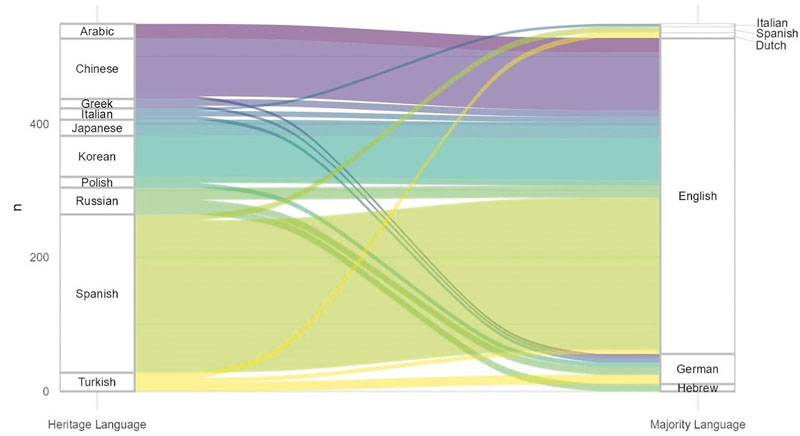
\includegraphics[width=\textwidth]{figures/iefremenko-img001.jpg}
\caption{\label{fig:key:1}: Top 10 subfields in HL research based on a literature survey (\citealt{FridmanÖzsoy2024})}
\end{figure}

\figref{fig:key:1} demonstrates that English is the most common majority language, with German coming in a distant second. Spanish is the most widely studied heritage language, followed by Chinese and Korean, all of which are primarily researched in the context of majority English. Other investigated heritage languages include Arabic, Greek, Italian, Japanese, Polish, Russian, and Turkish.

\section{Objectives and scope of this study}\label{sec:key:1.2}

In light of the current debates in heritage language research, this study aims to:

\begin{enumerate}
    \item Contribute to understanding and modeling heritage language grammars by considering the aforementioned proposals and examining factors such as CLI and internal dynamics in the languages, particularly the role of register.
    \item Expand the comparative framework by including bilingual majority speakers, thereby shifting the focus from a simple mono- versus bilingualism dichotomy to an analysis of the status of the languages under investigation (heritage vs. majority).
    \item Focus on the relatively frequently studied heritage language Turkish and the largely unexplored Kurmanji Kurdish within the context of the majority German and majority Turkish languages.
\end{enumerate}

To address these aims, the study examines two languages—Turkish and Kurmanji Kurdish—across four speaker populations: Turkish heritage speakers in Germany, Turkish-Kurmanji heritage speakers in Germany, Turkish-Kurmanji bilinguals in Turkey, and Turkish monolinguals in Turkey.

Let us discuss the objectives in reverse, beginning with the third. This study concentrates on two languages, Turkish and Kurmanji. While Turkish has been the subject of heritage language research—although primarily in the German context—Kurmanji Kurdish remains largely overlooked. This study investigates Kurmanji in two countries, Germany and Turkey. While Kurmanji is clearly recognized as a heritage language in the German context, its classification as such in Turkey is less common.

According to \citegen{Rothman2009} definition, a heritage language is one that is acquired early in life in a naturalistic setting but is not the dominant language of the wider society. Although this definition applies to many language constellations and minoritized languages around the world, as shown in the figure above, most heritage language research focuses on immigrant contexts in the Global North. Nevertheless, minoritized languages like Kurmanji Kurdish in Turkey exhibit the same characteristics described in Rothman’s definition of a heritage language. As will be discussed in Chapter \ref{chap:key:2}, Kurmanji is primarily acquired at home, while Turkish functions as the dominant language of the society. Consequently, Kurmanji speakers often have very limited exposure to their heritage language and lack opportunities for formal acquisition in educational settings (\citealt{BulutOpengin2018}). For this reason, Kurmanji in Turkey is classified as a heritage language in this study.

Nevertheless, several important differences must be considered. Unlike “classic” heritage languages, minoritized languages typically lack a corresponding majority variety, and their speakers are often bilingual or even multilingual. This makes comparisons feasible only among different groups of heritage speakers, whether based on age or between those who have different majority languages in contact. Additionally, minoritized languages frequently lack standardization and may not exhibit a wide range of registers \citep[323-324]{Polinsky2018}.

Furthermore, the contact between minoritized languages and the majority language in a given society is often longer and more intense than that of “classic” heritage languages in the Global North. In the field of language contact research, the intensity of contact—defined by the number of speakers in the community and the duration of contact—is considered a crucial social factor for predicting contact-induced language change: the more intense the contact, the greater the likelihood of structural changes (\citealt{ThomasonKaufman1988}). Thus, these differences will be taken into account in subsequent discussions throughout the study.

The second objective of this study is to broaden the comparative framework by incorporating bilingual majority speakers in Turkey whose first language is Kurmanji and whose second language is Turkish. This approach allows us to analyze two groups where Turkish serves as the majority language: monolingually and bilingually raised speakers. By incorporating these groups, the focus shifts from bilingualism itself to the status of the language being studied, whether it is a heritage or majority language. Furthermore, there are only a handful of studies on the Turkish spoken by Kurmanji-Turkish bilinguals in Turkey, and this study aims to establish a foundation for future research in this area.

Finally, the last objective of this study is to contribute to a better understanding of heritage language grammars and the factors that may account for the wide range of competences and performances observed among heritage speakers. This includes examining CLI influence and internal linguistic dynamics, with the focus on the role of register.

It is important to note that research on the factors shaping outcomes of languages in contact did not originate in heritage language studies, but in the broader field of contact linguistics. Within this field, linguists often differentiate between externally and internally motivated change \citep{Hickey2020}. Externally motivated changes, often referred to as instances of CLI, arise from contact with another language and result into the transfer of lexical or structural features from a dominant language (\citealt{jarvis_crosslinguistic_2008}, \citealt{ThomasonKaufman1988}, \citealt{Matras2009, Matras2020}). Internally motivated changes, in contrast, emerge from the language's own dynamics, including processes such as variation, generational transmission, and youth language (\citealt{Labov1994, Labov2001, Labov2010}, \citealt{PoplackLevey2010}, \citealt{Tagliamonte2016}).

The phenomenon of CLI is described using a variety of terms. It is often understood as the transfer of structures or forms from one language to another, and is commonly referred to as borrowing. Linguists typically distinguish between two main types of borrowing. The first involves the direct adoption of specific linguistic items, such as words or fixed expressions, from one language into another, and has been variously labeled “importation” \citep{Haugen1950}, “selective copying” \citep{Johanson2002}, or “matter replication” \citep{Matras2020}. The second type involves the borrowing of underlying grammatical and structural patterns or constructions, rather than just isolated lexical items. \citet{Haugen1950} refers to this as a “calque”, \citet{Johanson2002} as “global copying”, and \citet{Matras2020} as “pattern replication”. A related concept is “convergence” \citep{Weirich1953}, which can be understood as a mutual process or affect only one of the languages in contact \citep{Matras2020}. Throughout this study, the term \textit{cross-linguistic influence} will refer broadly to all types of contact-induced changes discussed above.

Understanding how language changes requires examining the underlying linguistic mechanisms. From the perspective of the usage-based approach, language is not simply a system of abstract rules but a dynamic inventory of patterns and constructions that emerge from actual use (\citealt{Bybee2010}, \citealt{langacker_foundations_1987}, \citealt{Dabrowska2019}). In this framework, constructions are grammatical units of varying size and complexity in which specific structural patterns are associated with particular functions or meanings. Constructions lie on a continuum from fully specific lexicalized units, such as idioms (kick the bucket) or prefabricated expressions (I don’t know), to highly schematic patterns, such as imperative forms or generalized argument structures (\citealt{langacker_foundations_1987}, \citealt{Goldberg2006}, \citealt{Nicolai2014}). Partially schematic constructions occupy the intermediate space, with some elements fixed and others open for lexical insertion. Structural change can therefore be understood as the cumulative outcome of how these constructions are stored, accessed, and generalized by speakers.

Frequency of use is a crucial factor in language change. Highly entrenched constructions are more resistant to modification and tend to be preserved over time, whereas less frequent or less entrenched constructions are more vulnerable to change or replacement (\citealt{langacker_foundations_1987}, \citealt{Tomasello2010}, \citealt{HakimovBackus2021}). In multilingual environments, speakers often generalize across their language repertoire, adopting structures present in multiple languages and producing shared constructions more frequently when the languages involved are similar and contact is prolonged (\citealt{Ansaldo2009}, \citealt{Matras2020}).

The usage-based approach also emphasizes the role of individual speakers in driving change. Language change is seen as the cumulative effect of repeated choices made during interaction: as constructions are repeatedly used by more speakers, they become more entrenched and can eventually lead to conventionalized patterns at the community level (\citealt{Nicolai2014}, \citealt{Bybee2006}). The propagation of innovations is gradual, and not all new constructions become conventionalized, the likelihood of adoption depends on factors such as directionality of bilingualism and social pressure to adhere to established norms \citep{Matras2020}.

Furthermore, structural and usage-based perspectives can be complemented by consideration of social factors, which have consistently been highlighted as primary determinants of language change. \citet{ThomasonKaufman1988} argue that while linguistic factors such as typological constraints can shape possible outcomes, it is the sociolinguistic context of the speakers that largely governs what changes occur and to what extent. Key social factors include imperfect learning, arising from incomplete acquisition of a target language, speakers’ attitudes toward the languages and the contact situation, and the intensity of contact, determined by both the number of speakers involved and the duration of the language contact. Intensity of contact influences the depth of linguistic change: in casual contact situations, borrowing is typically limited to content words, whereas in more intense contact situations, structural features—including word order, clause-combining strategies, and inflectional morphology—are more likely to be affected \citep{Thomason2022}.

Other influential factors include language dominance and prestige, the degree of bilingualism, and institutional support such as literacy, schooling, and media exposure (\citealt{Johanson2002}, \citealt{Matras2020}), the language user’s level of proficiency in the source language, as well as the frequency and recency of use of the post-L1 source language and its degree of similarity to the recipient language (\citealt{jarvis_crosslinguistic_2008}). Together, these factors shape both the features that are transferred and the direction of influence.

As noted earlier, CLI in heritage language research has received considerable attention. While contact between the heritage and the majority languages is undoubtedly ubiquitous, changes in the heritage language cannot always be attributed to CLI. Thus, \citet{FloresRinke2020} highlight another factor that should be taken into consideration and is often overlooked in the studies, namely language-internal phenomena of variation and variability. Even in monolingual varieties, language change can take place due to internal dynamics, including processes such as variation, analogical restructuring, generational transmission, and innovations in youth speech communities (\citealt{Labov1994, Labov2001, Labov2010}, \citealt{PoplackLevey2010}, \citealt{Tagliamonte2016}). \citet{FloresRinke2020} argue that heritage speakers may boost and further develop tendencies of language (internal) evolution inherent to variable phenomena. Furthermore, they may also retain variation that is typical of non-standard registers, because they are mainly exposed to colloquial input.

Building on these insights, this study focuses on the role of register in heritage language outcomes—a factor that has received relatively little systematic attention in heritage language research. In this study, register is defined as “those aspects of socially recurring intra-individual variation that are influenced by situational and functional settings” \citep[3]{ludeling_register_2022}. This means that patterns of variation are socially recurrent—speakers tend to adjust their language use in similar ways across comparable contexts. At the same time, this variation is fundamentally intra-individual: it is the same speaker who systematically varies their linguistic choices depending on the communicative setting. In this sense, register captures how socially structured patterns of language use are realized within individuals across different contexts. \citet{HallidayEtAl1964} and \citet{Halliday1989} distinguish between three components that serve as a model for understanding the situational-functional context of register: field, tenor, and mode. In this framework, the field relates to the subject matter or topic of discourse, the tenor involves social roles, relationships, and power dynamics among participants, while the mode refers to the channel of communication (spoken or written). \citet{Wiese2021} further highlights that such situational characteristics identify communicative situations.

Communicative situations will play a pivotal role in the methodology of the current study. In this context, the two defining parameters of communicative situations are formality and mode, each featuring two levels: informal versus formal and spoken versus written. The specific examples of the communicative situations used in the current study will be given in the Chapter \ref{chap:key:4}, Methodology.

From the above-given discussion on registers and communicative situations, it is evident that linguistic features constitute registers while situational characteristics define communicative situations. Consequently, register knowledge is the knowledge of the alignment of particular linguistic forms and structures with certain situations \citep{PescumaEtAl2023}. For instance, speakers may choose different structures depending on an interlocutor, the formality of the situation, the mode, the purpose of the conversation, etc.

Register can play an important role in understanding heritage speakers’ languages. As discussed at the beginning of this chapter, heritage speakers usually acquire their heritage language at home and often have limited exposure to formal registers in their heritage language. Many studies investigating heritage languages rely on data collected in informal settings, which is sometimes implicitly compared to the norms of the standard language of majority speakers. This approach can put heritage speakers at a disadvantage, as it overlooks the role of register in shaping language use.

\citet{WieseEtAl2022} emphasize the importance of selecting an appropriate baseline for comparison. Their findings show that noncanonical linguistic phenomena—features that deviate from standard norms—do occur in heritage language use, but crucially, they are also frequently observed in the informal speech of monolingually raised speakers of the same language.

Incorporating data elicited across different communicative situations into heritage language research is essential for ensuring fairer and more accurate comparisons between heritage and majority speakers. By accounting for register in both data collection and analysis, researchers can better isolate whether observed differences are truly due to heritage language development or simply reflect informal, nonstandard usage. Moreover, examining the informal speech of majority language speakers provides valuable insights into broader linguistic trends, including whether certain features associated with heritage speakers might actually reflect ongoing changes within the majority language itself.

The investigated linguistic phenomenon chosen for the study is word order, specifically the post-predicate position in Turkish and Kurmanji Kurdish. The rationale for concentrating on this position is that the languages under investigation here, Turkish, Kurmanji, and German, are SOV languages, yet they employ the post-predicate position to a different extent. Moreover, the employment of this position is determined by different factors in each language: information structure in Turkish (\citealt{Erguvanli1984}, \citealt{Erku1983}, \citealt{Issever2003}), predicate semantics in Kurmanji (\citealt{Gundogdu2019}, \citealt{Haig2018, Haig2020}), and syntactic structure in German (\citealt{Frey2015}, \citealt{Muller2023}).

Despite the differences across languages, several overlapping factors influence the use of the post-predicate position. \citet{Asadpour2021}, for instance, shows that in Mukri Kurdish spoken in Iran, information structure—alongside predicate semantics—affects word order. If similar patterns are found in Kurmanji Kurdish spoken in Turkey, this would suggest that information structure plays a shared role in both Kurmanji and Turkish. Additionally, factors such as mode and formality influence the use of post-predicate constituents in Turkish and German, where they are more common in spoken than written language, and in informal rather than formal situations (\citealt{Schroeder1995, Schroeder2002}, \citealt{Tsehaye2023}). Although the effect of mode and formality are underexplored in Kurmanji, evidence from related languages like Persian suggests they may be relevant (\citealt{Frommer1981, Haig_post-predicate_EtAl2024-1}). Thus, such differences and similarities create opportunities for interesting developments in these languages, driven by language contact.

The manuscript is organized as follows: Chapter \ref{chap:key:2} introduces the communities investigated in this study. Chapter \ref{chap:key:3} discusses word order in Turkish, Kurmanji, and German, providing an overview of previous research on the post-predicate position in these languages. After establishing the theoretical background, Chapter \ref{chap:key:4} outlines the methodology, participants, corpus, and details of the analysis process. Chapters \ref{chap:key:5} and \ref{chap:key:6} present the results for Turkish and Kurmanji, respectively. Chapter \ref{chap:key:7} addresses the research objectives, examines CLI, internal dynamics, and the role of register, and discusses the study’s limitations. Chapter \ref{chap:key:8} offers a concluding overview.


\chapter{Turkish and Kurmanji in Germany and Turkey}\label{chap:key:2}
\section{Turkish as a heritage language in Germany}\label{sec:key:2.1}

Turkish is one of the largest immigrant communities in Germany, with nearly five million speakers of the Turkish language (\citealt{KaranfilŞavk2013}). Although migration from Turkey to Germany began approximately 60 years ago, and many Turkish families now reside in Germany for three or even four generations, the Turkish language continues to be regarded as a relatively vital language. Turkish speakers maintain their language due to several factors, including the presence of numerous religious and social institutions where Turkish is regularly spoken, easy access to Turkish media, ongoing contact with Turkey, and a relatively low rate of exogamous marriages \citep{Bhatia2004}.

In cities with large Turkish-speaking populations, such as Berlin, Cologne, and Frankfurt, people can use Turkish not only at home with family but also in informal public settings, including shops, cafes, and during leisure activities (\citealt{Hottmann2008}, \citealt{IefremenkoEtAl2021}). Furthermore, studies on language orientation within Turkish communities in Western Europe and Australia (\citealt{Yagmur2004}, \citealt{YagmurVanDeVijver2012}) have found that the Turkish community in Germany exhibits the highest levels of ethnic identification and the lowest levels of mainstream identification among the communities studied. This strong sense of ethnic identity contributes to the vitality of the Turkish language.

Immigration from Turkey to Germany began in the 1960s with a recruitment agreement between the two countries, allowing Turks to come to Germany as \textit{Gastarbeiter}, or `guest workers.' These individuals were primarily male laborers with little to no vocational training, originating from rural areas throughout Turkey \citep{Bayram2013}. Under the initial agreement, workers were expected to stay for only a short period before returning to their homeland. However, in the early 1970s, the law changed, permitting guest workers to remain in Germany and reunite with their families \citep{Angin2003}. This reunification policy led to a rapid increase in the size of the Turkish community in Germany and transformed the demographic composition from predominantly male workers to families with children \citep{Bayram2013}.

At the beginning of the guest workers' stay in Germany, they were regarded as temporary residents, leading to minimal efforts to facilitate their integration into German society. Furthermore, it was unclear whether schooling should be compulsory for children of guest workers \citep{Beck1999}. Subsequently, various educational models were adopted by different German states. For instance, Berlin placed foreign children, including those born in Germany, in \textit{Ausländerregelklassen} (`preparatory German language classes') due to their insufficient proficiency in German \citep{Pfaff1991}. In contrast, Bavaria and Baden-Württemberg implemented \textit{Muttersprachenunterricht} (`mother tongue education'), allowing children to study the history, arts, culture, geography, and religion of their parents’ country of origin \citep{Damanakis1983}. The primary aim of these classes was to prepare children for easier integration should they return to Turkey \citep{Damanakis1983}. However, both models ultimately failed, further hindering immigrant children’s integration into German society and their access to professional education \citep{Beck1999}.

The current situation for children who speak a language other than German at home has changed significantly. These children now start elementary school alongside their monolingually raised peers and, over time, often become more proficient in German than in their heritage language. As a result, the heritage language typically receives input only in the home environment, placing it at a disadvantage.

To help support heritage language development, some schools offer dedicated classes. For example, Turkish heritage language classes are provided by consulates or federal states in every German state where heritage language education is available. However, unlike long-established foreign languages such as Spanish or French, Turkish is rarely taught as a regular foreign language in Germany. Instead, it is more commonly offered as a language of origin in the context of family language classes. At the elementary level, Turkish is typically taught as \textit{Herkunftssprachenunterricht} (`heritage language instruction') or \textit{muttersprachlicher Ergänzungsunterricht} (`additional mother tongue teaching'), continuing until the end of grade 4 (and until the end of grade 6 in states such as Berlin and Brandenburg) \citep{KuppersEtAl2014}.

Only a few states, including North Rhine-Westphalia, Berlin, Bremen, Hamburg, Bavaria, and Lower Saxony, offer Turkish language instruction as a second or third foreign language at the lower and upper secondary levels \citep{KuppersEtAl2014}. Additionally, some states, such as North Rhine-Westphalia, Hamburg, and Bremen, provide Turkish as a foreign language (TaF), however, this option is rarely implemented due to a shortage of trained teachers \citep{Schroeder2003}.

\largerpage
The vitality of the Turkish language in Germany, coupled with the large Turkish population, has led to a significant increase in studies investigating Turkish as spoken in Germany. These studies have explored various linguistic domains of heritage Turkish and found that it often differs from the Turkish spoken in Turkey. For instance, in the domain of phonology, \citet{Queen2001} identified a novel intonation pattern used by Turkish-German bilingual children in both their Turkish and German. The researcher argues that this novel intonation pattern results from the fusion of German and Turkish prosodic features. Similarly, \citet{Kuhn2019} discovered that heritage speakers of Turkish tend to transfer functionally related prosody from German into Turkish, thereby contributing to the contextualization of pragmatic concepts that are not expressed through other linguistic means in Turkish. In morphology, evidence from studies on Turkish heritage speakers in Germany comes primarily from real-time processing experiments. Heritage speakers generally perform similarly to monolingually-raised Turkish speakers in processing derived and inflected morphologically complex words (\citealt{JacobKırkıcı2016}, \citealt{JacobEtAl2019}), regular and irregular aorist verbs (\citealt{UygunClahsen2021}, \citealt{UygunEtAl2023}), grammatical aspect (\citealt{BuyukyildirimEtAl2025}), showing sensitivity to imperfective and perfective distinctions, and grammatical case \citep{OzsoyEtAl2023}. At the same time, they exhibit greater variability with irregular forms, such as irregular aorist verbs (\citealt{UygunClahsen2021}). Comprehension is also influenced by individual factors, with higher language proficiency and faster processing speed associated with higher accuracy rates (\citealt{BuyukyildirimEtAl2025}). Evidence from morphosyntax, by contrast, highlights differences between heritage and majority speakers. For example, heritage speakers in Germany tend to overuse overt subjects compared to monolinguals in Turkey and heritage speakers in the U.S. \citep{OzsoyEtAl2025}. Similarly, \citet{Uygun2022} shows that heritage speakers overuse plural-marked verbs in optional subject-verb agreement contexts. In the domain of syntax, studies have shown that hypotactic means of clause combining are less frequent in Turkish spoken in Germany compared to that in Turkey (\citealt{Treffers-dallerEtAl2006}, \citealt{Bayram2013}, \citealt{IefremenkoSchroeder2019}, \citealt{Schroeder2025}). Conversely, some research indicates a higher frequency of paratactic clause combining in Turkish in Germany compared to majority Turkish (\citealt{Dollnick2013}, \citealt{Guven2016}) and the emergence of novel coordinators in heritage Turkish in Germany (\citealt{Herkenrath2007}, \citealt{Karakoç2007}, \citealt{HerkenrathKarakoc2007}, \citealt{Csato2016}, \citealt{OzsoyEtAl2022}, \citealt{IefremenkoOezsoySchroeder2024}). These differences suggest that heritage speakers may develop new clause combining strategies, likely under the influence of the majority language.

\newpage
In summarizing some of these studies, \citet[34]{KuppersEtAl2015} suggest that the observed changes across different linguistic domains in heritage Turkish in Germany “could potentially be considered characteristics of an emerging new variety: ‘Germany Turkish’.”

\section{Kurmanji as a heritage language in Germany}\label{sec:key:2.2}

An interesting fact of the Turkish migrant population in Germany is that a significant number of these individuals are actually ethnic Kurds. As previously noted, the first wave of immigration began in the 1960s, when primarily male workers from Turkey arrived in Germany as guest workers. The second wave of Kurdish migration to Western Europe occurred in the 1980s, largely consisting of asylum seekers fleeing Turkey \citep{Ostergaardnielsen2001}. Kurdish migration to Germany has continued to the present day, driven by factors such as family reunification, job relocation, and asylum seeking (\citealt{DemmrichArakon2021}, \citealt{Mcgee2018}). Despite their ethnicity, migrants from Turkey are often classified as Turks based solely on their country of origin. Today, there are approximately 1,300,000 Kurds living in Germany (\citealt{GhaderiAlmstadt2023}). However, it remains unclear how many of these individuals identify as Kurds and what language(s) they speak at home.

The situation regarding Kurdish heritage education is complex for several reasons. First, Kurds do not have an officially recognized state, with their population dispersed across countries such as Turkey, Iran, Iraq, and Syria. This raises the issue of which consulate would be responsible for providing Kurdish heritage language education in Germany, particularly since Turkish is the only official language in Turkey. Secondly, Kurdish is a macro-language that encompasses a continuum of languages that are not fully mutually intelligible (\citealt{Hassanpour1992}, \citealt{Sheyholislami2015}). The differences among Kurdish languages are further exacerbated by the fact that they are written in at least three different scripts: the Latin-based alphabet used by Kurds in Turkey (and some in Syria), the Arabic-based alphabet employed by Kurds in Iran and Iraq, and the Cyrillic alphabet used by Kurdish speakers in countries of the former USSR \citep{Sheyholislami2009}. Consequently, it is essential to determine which variant of the Kurdish language should be taught to Kurdish children in Germany. Finally, the lack of trained Kurdish teaching staff poses an additional challenge, as there are currently no departments in German universities that offer teacher training programs specifically for Kurdish educators.

\newpage
Despite these challenges, heritage Kurdish education is offered in several German states. The initiative began in the early 1990s in Lower Saxony, followed by the city-states of Bremen and Hamburg \citep{Schmidt2000}. Currently, Kurdish language education is available in Brandenburg, Bremen, Lower Saxony, North Rhine-Westphalia, and Rhineland-Palatinate (\citealt{Mediendienst2019}). In 2019, the Berlin Senate approved the introduction of Kurdish classes at three schools in Berlin \citep{Derince2022}.

However, the absence of a standardized Kurdish language raises the ongoing issue of which language or dialect to teach. Different federal states have proposed various solutions to address this challenge. For instance, in Bremen, most families whose children participate in Kurdish mother tongue lessons are immigrants from Mardin, Turkey \citep{Schmidt2000}. As a result, researchers and Kurdish language teachers decided to instruct children in the variety most commonly spoken at home. In Lower Saxony, parents were asked to complete a questionnaire regarding their preferred variety for their children's instruction \citep{Schmidt2000}. In Hamburg, although the Kurdish community is quite heterogeneous, Kurdish lessons are organized exclusively for Kurmanji speakers, as the Sorani-speaking population is more dispersed throughout the city \citep{Schmidt2000}.

Probably due to the challenges mentioned earlier, only a limited number of studies have focused on heritage Kurmanji in Germany. One of the few studies examining Kurmanji-Turkish-German trilinguals in Germany, conducted by \citet{Herkenrath2021}, investigates the use of post-predicate elements across the three languages in contact, noting that the employment of the post-predicate position is influenced by various factors: discourse planning and information structure in Turkish, argument structure in Kurmanji, and syntactic structure in German. The researcher observes that the reasons for using the post-predicate position in the languages studied overlap, which can be attributed to their mutual influence through language contact. This exploratory study highlights the need for a more comprehensive investigation of ongoing changes in heritage Kurmanji.

In addition to this research, a small body of studies on Kurmanji in contact with German has addressed issues such as child language acquisition, particularly in preschool-age learners in Germany (\citealt{Kirgiz2022}), literacy acquisition (\citealt{Simsek2016}, \citealt{CorvachoEtAl2021}), language education \citep{Derince2022}, and sociological factors \citep{Eccarius2019}.

Moreover, it is noteworthy that many members of the Kurmanji-speaking population in Germany, whose ancestors immigrated from Turkey, are often able to speak Turkish. For various reasons, Kurmanji-Turkish-speaking parents in Germany may expose their children to both Kurmanji and Turkish. This exposure is frequently attributed to the high vitality of the Turkish language in Germany and its presence in informal public contexts. As a result, children may be raised trilingually, speaking Kurmanji and Turkish at home and in the neighborhood while using German as the majority language in the broader community.

Therefore, when discussing Turkish as an emerging variety in Germany, it is essential to include both Turkish-German bilinguals and Turkish-Kurmanji-German trilinguals in the analysis. To better understand the underlying factors contributing to potential changes, it is crucial to distinguish between these two groups, which will be addressed in the current study.

\section{Kurmanji as a heritage language in Turkey}\label{sec:key:2.3}

As evident from the previous discussion, the contact between Turkish and Kurmanji did not originate in Germany. For centuries, Kurds have lived in a multilingual environment, resulting in the Kurdish language maintaining close contact with various languages, including Arabic, Aramaic, Persian, and Turkish. During the Ottoman Empire, all nations were able to preserve and develop their languages. However, following the establishment of the Republic of Turkey in 1923, significant changes were made to language policy (\citealt{Yagmur2001}). At that time, the Turkish language—specifically the standard variety known as Istanbul Turkish—became the central focus of language policy in the newly formed country. This policy aimed to promote linguistic homogeneity and national unity by establishing Turkish as the sole official language.

The implementation of a single official language led to the marginalization of linguistic diversity in Turkey. As \citet{Yagmur2001} notes, the majority of linguistic minority groups assimilated into the mainstream community. However, due to their significant population and geographic isolation, Kurdish communities managed to maintain their languages (\citealt{Yagmur2001}). \citet{Dorleijn1996} also indicates that in some rural towns in southeastern Turkey, Kurdish served as a \textit{lingua franca} among speakers, including native Turkish speakers, during the 1990s. Consequently, this study emphasizes that Kurmanji can be considered a heritage language, provided that the language is not widely used in public contexts and the majority of the population does not speak Kurmanji.

The situation surrounding the education of Kurmanji in Turkey has undergone significant transformations over the past century. For more than half of the 20th century, there was a concerted campaign aimed at assimilating ethnic minorities into Turkish society, promoting ethnic mixing through both voluntary and forced migration. During this time, the use of Kurmanji faced severe restrictions, it was not only prohibited in education and broadcasting by law but also banned in everyday speech (\citealt{Zeydanlioglu2012}).

However, the 1990s marked a slight shift in this trend, as Kurmanji was no longer classified as a prohibited language. Radio and television broadcasting, as well as the publication of newspapers and books in Kurmanji, were gradually permitted again, albeit with certain restrictions \citep{Derince2013}. Starting in 2003, private courses for teaching Kurmanji were allowed, but these courses were limited to just 10 weeks, with a maximum of 18 hours per week, and were available only for adults (\citealt{Zeydanlioglu2012}).

In 2012, further reforms enabled middle school students (grades 5--8) to choose Kurmanji as an elective course in Turkish public schools (\citealt{Arslan2015}, \citealt{Derince2013}). This course could be taught for only two hours per week and would only be offered if enough students expressed interest. However, in recent years, the teaching of Kurmanji in Turkey has faced some challenges and limitations, which have affected the use and development of the language within the formal education system.

Although the contact between Turkish and Kurmanji has lasted longer than that between Turkish and German, there is a limited number of studies exploring the CLI between the former pair. One notable study by \citet{JohansonTurkyilmaz2006} investigated the influence of Turkish on Kurmanji phonology, finding that the contact of the Sinemili dialect of Kurmanji with Turkish has led to the extensive use of front rounded vowels by speakers of this dialect. Research has also documented instances of lexical borrowing from Turkish into Kurmanji, as shown in studies by \citet{Bulut2006}, \citet{Dorleijn1996, Dorleijn2006}, and \citet{Cabuk2020}. Furthermore, CLI from Turkish on Kurmanji has been observed in the realm of morphology. For instance, \citet{Dorleijn1996} analyzed the speech of two Kurmanji-Turkish bilinguals from Diyarbakır, revealing a significant impact of Turkish on Kurmanji across all linguistic domains, particularly in morphology. This influence was evident through the adoption of Turkish possessive suffixes in Kurmanji, the loss of gender distinctions, and the omission of overt subjects, among other changes. Additionally, \citet{Cabuk2019} noted the borrowing of the Turkish suffix \textit{-mış} into Kurmanji, which loses its original evidential and perfective meanings in the process.

A comprehensive study by \citet{Haig2007} examined the potential influence of Turkish on the Tunceli dialect of Kurmanji across various linguistic domains. The researcher identified instances of lexical borrowing, including discourse markers, conjunctions, and relational nouns. \citet{Haig2007} also suggested that some structural changes in Kurmanji due to Turkish influence are evident in specific constructions, such as those involving the verb \textit{bûn} (‘to be’), used in both static and processual senses. Nevertheless, the author concludes that despite centuries of coexistence between Kurmanji and Turkish speakers, the core grammar of both languages remains distinct \citep{Haig2007}.

\largerpage
Thus, existing studies on the language contact between Kurmanji and Turkish have predominantly focused on the impact of Turkish on Kurmanji, while the influence of Kurmanji on Turkish has received less attention in academic research. One study by \citet{PolatSchallert2013} examined the attainment of a “native-like” Turkish accent among L1 Kurmanji-speaking adolescents in a Turkish-dominant city. The study revealed considerable variation in the accents of the bilingual speakers in their Turkish. The findings indicated that the degree of identification with the Turkish-speaking community positively predicted a “native-like” Turkish accent. Additionally, \citet{Yonat2023} explored the influence of Kurmanji on Turkish in the realm of phonology, uncovering instances of sound transfer from Kurmanji to Turkish. This study showed that sounds characteristic of Kurmanji were incorporated into the Turkish spoken by Kurmanji speakers. The author emphasizes that the Turkish used by Kurmanji speakers differs from Standard Turkish and posits that it represents a distinct native variety within the Turkish language. Furthermore, \citet{Aykac2016} identified several instances of construction copying from Kurmanji into Turkish in the written texts of Kurmanji-speaking students. For example, the author notes that constructions featuring the reflexive pronoun \textit{kendi} (‘own, self’), such as \textit{kendime kitap okuyorum} (literally, ‘I’m reading a book to myself’), are common in the speech of Kurmanji-Turkish bilinguals. In contrast, the same sentence in standard Turkish would typically be expressed without the reflexive pronoun, as in \textit{kitap okuyorum} (‘I’m reading a book’). Aykaç further suggests that such constructions are transferred from Kurmanji, where the reflexive pronoun \textit{xwe} is required in the same context, as demonstrated in the sentence \textit{ez ji xwe re kitêb dixwînim} (‘I’m reading a book’). The author identifies over twenty such constructions in total and argues that they have gradually gained wider currency within the community, to the extent that they are now also used by speakers without a Kurmanji background. From a usage-based perspective, \citet{Aykac2016}'s findings suggest that the adoption of these novel constructions by a larger number of speakers has resulted in greater entrenchment of these forms in the mental representations of individuals, which has, in turn, facilitated the propagation of these constructions throughout the community.

Finally, although there are almost no studies that systematically investigate the societal perception of the Turkish language spoken by bilingual speakers in Turkey, a bias exists within society toward Kurmanji-Turkish bilinguals, particularly regarding the belief that their language does not conform to the norms of Standard Turkish (\citealt{DemirciKleiner1999}). \citet{Tulgar2010}, as noted in \citet{Inal2019}, highlights the ongoing discrimination against Kurds due to the phonetic peculiarities in their Turkish. For example, \citet{Sahin-firat2010} conducted interviews with Kurdish students, some of whom shared experiences of anxiety related to being made fun of because of their pronunciation in Turkish, or the embarrassment they felt when their parents spoke Turkish with an accent at school.

\section{Summary}\label{sec:key:2.4}
\largerpage
This chapter has outlined the sociolinguistic and educational contexts in which Turkish functions as a heritage language in Germany, Kurmanji is a heritage language in Germany and Turkey, and Turkish as a majority language of monolingual and bilingual speakers in Turkey. The overview demonstrates that both languages exist in complex contact situations that often go beyond bilingualism, involving not only two but sometimes three languages in contact, as in the case of Kurmanji-Turkish-German speakers.

The speaker groups under investigation also differ in the intensity of language contact, which can be assessed in terms of both its duration and the size of the communities involved. In Germany, contact between Turkish or Kurmanji and the dominant language German began in the second half of the twentieth century with the arrival of the so-called guest workers. In contrast, contact between Turkish and Kurmanji started before the Ottoman Empire and intensified following the establishment of the Turkish Republic, when Turkish became the country’s sole official language (\citealt{Yagmur2001}). In addition, the Turkish-speaking community in Germany constitutes one of the largest immigrant groups, particularly in Berlin, where the present study’s data were collected. The number of trilingual Kurmanji-Turkish-German speakers, by comparison, is considerably smaller and not precisely known, while the number of Kurdish speakers in Turkey far exceeds that of immigrant communities in Germany. Thus, considering both the duration of contact and community size, the speaker groups in Germany stand in contrast to the Kurmanji-Turkish bilingual group in Turkey investigated in this study.

Finally, the status of the languages under investigation differs across contexts. In Germany, both Turkish and Kurmanji function as heritage languages, in Turkey, Kurmanji can also be considered a heritage, and Turkish serves as the majority language of both monolingual and bilingual speakers. 

Taken together, the sociolinguistic profiles and contact histories discussed in this chapter highlight the diversity of contact settings in which Turkish and Kurmanji are used. Examining CLI across these different groups provides an opportunity to explore how, in addition to linguistic factors, social factors such as language status and the intensity of contact shape the linguistic outcomes of both heritage and majority speakers.


\chapter{Word order in the investigated languages}\label{chap:key:3}

The word order in the three languages under investigation -- Turkish, Kurmanji Kurdish, and German -- is SOV. However, each language also allows certain constituents to appear in the post-predicate position. The use of this position is influenced by different factors: information structure in Turkish, predicate semantics in Kurmanji, and syntactic structure in German. At the same time, there are overlaps in the factors that govern the placement of constituents in the post-predicate position.

Importantly, constituents in the post-predicate position can be clausal and non-clausal. This study focuses specifically on non-clausal post-predicate constituents. The rationale behind this decision is that including clausal constituents would involve the discussion of clause-combining, which is a different, although definitely related, topic.

This chapter provides a detailed overview of word order in the three languages, with a particular focus on non-clausal post-predicate constituents. Additionally, relevant studies on word order in these languages in contact situations are summarized.

\section{Word order in Turkish} \label{sec:key:3.1}

Turkish is considered to have a relatively free word order, with the basic word order being SOV (\citealt{Erguvanli1984}: 5, \citealt{GokselKerslake2004}: 343-346). This implies that even though word order variation is possible, there are certain instances where the word order must remain fixed. One such case occurs when noun phrases lack case marking and there are no semantic cues to distinguish their grammatical roles, as illustrated in the following examples (\citealt{Erguvanli1984}: 5):

\ea\label{ex:key:1} Turkish (\citealt{Erguvanli1984}: 5)\\
\gll Mutluluk   huzur    getir-ir.\\
happiness  serenity  bring\textsc{-aor.3\textsc{sg}}\\
\glt ‘Happiness brings serenity.’
  \z

\ea%2
  \label{ex:key:2} Turkish (\citealt{Erguvanli1984}: 5)\\
\gll Huzur     mutluluk   getir-ir.\\
serenity          happiness         bring\textsc{-aor.3\textsc{sg}}\\
\glt ‘Serenity brings happiness.’
  \z

Variation in word order in Turkish is employed to serve pragmatic purposes, such as signaling topics and distinguishing between old and new information (\citealt{Erku1983}, \citealt{Erguvanli1984}: 44-50, \citealt{Issever2003}). Thus, word order in Turkish is strongly governed by information structure, where topicalized information appears sentence-initially, new information occurs immediately before the verb, and backgrounded information can be placed post-verbally (\citealt{Erku1983}, \citealt{Erguvanli1984}, \citealt{Hoffman1995}). For instance, the example \REF{ex:key:3a} below has pragmatically neutral unmarked order, whereas examples (3b--f) are pragmatically marked.



\ea\label{ex:key:3} Turkish, self-constructed \\
\ea\label{ex:key:3a}
\gll Murat     araba-yı   sat-tı.\\
Murat    car-\textsc{acc}  sell-\textsc{pst}.3\textsc{sg}\\
\glt ‘Murat sold the car.’\jambox*{SOV}

\ex\label{ex:key:3b}
\gll Araba-yı  Murat    sat-tı.\\
car-\textsc{acc}  Murat    sell-\textsc{pst}.3\textsc{sg}\\
\glt ‘It is Murat who sold the car.’\jambox*{OSV}

\ex\label{ex:key:3c}
\gll Murat    sat-tı    araba-yı.\\
Murat    sell-\textsc{pst}.3\textsc{sg}  car-\textsc{acc}\\
\glt ‘Murat did sell the car.’\jambox*{SVO}

\ex\label{ex:key:3d}
\gll Araba-yı   sat-tı     Murat.\\
car-\textsc{acc}  sell-\textsc{pst}.3\textsc{sg} Murat\\
\glt ‘It is the car that Murat sold.’\jambox*{OVS}

\ex\label{ex:key:3e}
\gll Sat-tı     Murat     araba-yı.\\
sell-\textsc{pst}.3\textsc{sg}  Murat    car-\textsc{acc}\\
\glt ‘Sell is what Murat did to the car.’\jambox*{VSO}

\ex\label{ex:key:3f} 
\gll Sat-tı     araba-yı   Murat.\\
sell-\textsc{pst}.3\textsc{sg}  car-\textsc{acc}  Murat\\
\glt ‘Sold the car is what Murat did.’\jambox*{VOS}
\z
\z


As shown in the examples above, scrambling in Turkish can result in certain constituents being placed in the post-predicate position, typically to background them. This backgrounding occurs under specific conditions: when the elements are discourse-predictable (i.e., previously mentioned or easily inferable from context) or supplementary (providing less crucial information for the listener) (\citealt{Erguvanli1984}). Consequently, information in the post-predicate position can often be omitted \citep{Hoffman1995}. Moreover, elements in this position are never stressed, as indicated by their flat and low intonation contour \citep{Kornfilt1997}.

Post-predicate constituents in Turkish may be of several types: noun phrases (NPs), adverbs, connectors, discourse markers, as well as subordinate clauses (\citealt{AkanHartmann2019}, \citealt{Erguvanli1984}, \citealt{Kornfilt1998}, \citealt{GokselKerslake2004}). Furthermore, there is no restriction on the number of constituents that occur after the predicate, and the order of the constituents after the predicate appears to be more flexible compared to the order of constituents in the pre-predicate position \citep{Skopeteas2015}. However, certain constituents are always placed in the post-predicate position. These are, for example, discourse markers that emphasize the preceding verb or the whole utterance but do not receive stress themselves. Thus, in example \REF{ex:key:4}, the discourse marker \textit{ki} emphasizes the whole utterance and follows the verb immediately.


\ea%4 
  \label{ex:key:4} Turkish, self-constructed \\
  \gll Ben  bun-u    yap-ma-dı-m    ki.\\
 I  this-\textsc{acc}  do-\textsc{neg-pst-1sg}  \textsc{dm}\\
 \glt  ‘But I haven’t done this!’ 
  \z

Nevertheless, there are restrictions on the types of constituents that may be placed in the post-predicate position (\citealt{Erguvanli1984}, \citealt{GokselKerslake2004}). Focus constituents, contrastive elements, new concepts, and unactivated topics do not appear in the post-predicate position in Turkish (\citealt{Erguvanli1984}, \citealt{Schroeder1995}). For example, no question constituent can be placed after the predicate because they are always focused.


\ea \label{ex:key:5} Turkish, self-constructed \\
\ea[]{\label{ex:key:5a}
   \gll Anahtar-ı san-a kim ver-di? \\
        key\textsc{-acc} you-\textsc{dat} who give-\textsc{pst.3\textsc{sg}}\\
   \glt ‘Who gave you the keys?’
}
\ex[*]{\label{ex:key:5b} 
   \gll Anahtar-ı san-a ver-di kim?\\
        key\textsc{-acc} you-\textsc{dat} give-\textsc{pst.3\textsc{sg}} who\\
        \glt Intended: ‘Who gave you the keys?’
} 
\z
\z


In example \REF{ex:key:5a}, the question word \textit{kim} ‘who’ appears immediately before the verb due to its focus. In contrast, example \REF{ex:key:5b} would be considered noncanonical, as placing the question word in the post-predicate position would background it -- an impossible structure in interrogative sentences.

Another restriction is that indefinite NPs cannot occur in the post-predicate position because they usually contain new information (\citealt{Erguvanli1984}). Consider the following examples:

\ea%6
  \label{ex:key:6}  Turkish, self-constructed \\
\ea[]{\label{ex:key:6a}
 \gll Dün    bir  kitap  al-dı-m \\
 yesterday  \textsc{art}  book  buy-\textsc{pst-1sg}\\
\glt ‘Yesterday I bought a book.’ 
 }
\ex[*]{\label{ex:key:6b}
\gll Dün    al-dı-m   bir  kitap\\
 yesterday  buy-\textsc{pst-1sg}  \textsc{art}  book \\
}
\z
\z

Thus, in example \REF{ex:key:6a}, the indefinite NP \textit{bir kitap} ‘a book’ is placed in the immediate preverbal position because in this sentence it is focused, whereas example \REF{ex:key:6b} with \textit{bir kitap} ‘a book’ in the post-predicate position would be considered noncanonical.

Nevertheless, under some conditions, new information can occur also in the post-predicate position. These instances are usually afterthoughts. An afterthought is a prosodically and syntactically independent unit, whose discourse function is to repair an unclear reference (\citealt{Benz2008}). \citet{Erguvanli1984} notes that in Turkish there is usually a slight pause between a predicate and an afterthought. Another indicator of an afterthought in Turkish is the word \textit{şey} `thing' positioned before the verb, serving as a placeholder for the material that appears as an afterthought. An example for this comes from \citet[51]{Erguvanli1984}:


\ea%7
  \label{ex:key:7} Turkish (\citealt{Erguvanli1984}: 51)\\
\gll Koca-sı    şey-de    çalış-ıyor    fabrika-da \\
 husband-\textsc{poss}.3\textsc{sg}  thing-\textsc{loc}  work-\textsc{prs}.3\textsc{sg}    factory-\textsc{loc}\\
\glt ‘Her husband works at-the-what-do-you-call-it, at the factory.’
  \z

Thus, in the example \REF{ex:key:7}, \textit{şey} signals that the location is being added as an afterthought, with the actual referent (\textit{fabrikada} ‘at the factory’) provided postverbally.

Furthermore, when the whole utterance is new, there may be post-predicate elements that are backgrounded in relation to the whole utterance. Besides, when there are several new constituents, the “less important” one can be placed in the post-predicate position. This often occurs when there is no intention to bring attention or emphasis to that particular constituent (\citealt{Kilicaslan2004}, \citealt{DogruozBackus2007}, \citealt{AkanHartmann2019}, \citealt{Issever2019}). An example for this is provided in \citet[204]{DogruozBackus2007}:


\ea%8
  \label{ex:key:8} Turkish (\citealt{DogruozBackus2007}: 204)\\
       Seza:
       \gll Türkçe-yi nerde öğren-di-n? \\
  Turkish-\textsc{acc} where learn-\textsc{pst}-\textsc{2sg}\\
 \glt  ‘Where did you learn Turkish?’

Seren:
\gll  O da aile-m-den sonra ilkokul-da hep Türk okul-u-na gid-il-di hafta-da bi defa.\\
  that \textsc{dm} family-\textsc{poss}.\textsc{1sg}-\textsc{abl} then primary.school-\textsc{loc} always  Turkish school-\textsc{poss}.\textsc{3sg}-\textsc{dat} go-\textsc{pass}-\textsc{pst} week-\textsc{loc} one time. \\
\glt ‘That is also from family, then we went to Turkish school during primary school once a week.’
  \z

In Example \REF{ex:key:8}, the postverbal element \textit{hafta-da bi defa} ‘once a week’ conveys new information and would therefore be expected to appear in the preverbal area. However, \citet{DogruozBackus2007} show that monolingually raised Turkish speakers in Turkey do not treat this as a violation, suggesting that the ban on postverbal focused elements is not as strict as previously assumed. Moreover, the authors show that similar examples can also be found in Turkish spoken in Turkey.

\subsection{The effect of formality and mode on the use of the post-predicate position} \label{sec:key:3.1.1}

Importantly, while post-predicate placement is not inherently noncanonical in Turkish, its usage is influenced by factors such as formality and mode. Sentences with post-predicate constituents are found in both written and spoken Turkish (\citealt{Antonova-unlu2015}). However, their usage is significantly more common in unplanned spoken discourse than in structured written texts (\citealt{Schroeder1995, Schroeder2002}, \citealt{Erdal1999}). This is because spoken discourse is typically spontaneous, often including afterthoughts and self-corrections. The post-predicate position aids listeners in keeping track of topic development and the deictic context in which the predication occurs \citep{Schroeder1995}.

Furthermore, \citet{Erguvanli1984} emphasizes that formality significantly influences the use of post-predicate structures. In highly formal styles of Turkish, such as legal documents and news items—whether written in newspapers and journals or broadcast on radio and TV—these structures are exceedingly rare. This rarity stems from normative pressures on the use of post-predicate structures in the formal language. A key factor behind this restriction is the politicized nature of the Turkish language in Turkey, any deviation from the standard sentence structure is often perceived as a foreign influence and met with resistance (\citealt{Erdal1999}, \citealt{KucukEtAl2017}).

In summary, word order in Turkish, and particularly the employment of the post-predicate position, is driven by the information structural requirements. This position is reserved for background information, hence, focused and new information is generally not allowed in this position. Moreover, mode (spoken vs. written) and formality (formal vs. informal) play a role in the employment of the post-predicate position. This position is characteristic of informal, unplanned spoken discourse, whereas its use is constrained by normative rules in formal settings.

\section[Post-predicate position in {Turkish} in language contact situations]{Studies on the post-predicate position in {Turkish} in language contact situations}\label{sec:key:3.2}

The use of the post-predicate position in Turkish has captured the attention of researchers, both in monolingual and multilingual contexts. While previous studies generally confirm that Turkish predominantly follows SOV word order, the reported proportions of pre- vs. post-predicate structures vary significantly across different datasets.

\largerpage
For instance, \citet{Saginsimsek2016} analyzed the speech of monolingual children in Turkey aged 2 to 6 and found that the frequency of post-predicate structures increases with age, rising from 15.9\% in 2-year-olds to 27.1\% in 5- to 6-year-olds. In another study, \citet{Antonova-unlu2015} examined spoken narrations of English-Turkish simultaneous bilingual\footnote{In the referenced studies, Antonova-Ünlü distinguishes between simultaneous and sequential bilingual acquisition. Simultaneous bilingual acquisition occurs when a child is exposed to two languages from birth or within the first week of life. In contrast, sequential bilingual acquisition refers to the situation in which an individual begins exposure to a second language later in life, after having already developed some proficiency in their first language. In \citet{Antonova-unlu2019}, the age of onset for the children learning Turkish ranged from 3 years and 1 month to 6 years and 4 months.} and Turkish monolingual children in Turkey, finding that both groups overwhelmingly favored verb-final word order, with 94--98\% of utterances conforming to this pattern. However, \citet{Antonova-unlu2019} also found that sequential bilingual children, after approximately 2--3 years of exposure to Turkish, used significantly more post-predicate structures than both monolingual and simultaneous bilingual children. Notably, these sequential bilinguals placed indefinite noun phrases or adverbials containing new and/or focused information in the post-predicate position, which deviates from the standard constraints of Turkish. In contrast, all instances of post-predicate use among monolingual and simultaneous bilingual children were rated as canonical. These results indicate that in child language, post-predicate placement is typically canonical for monolingual and simultaneous bilingual children, while sequential bilinguals show more flexibility, placing new or focused information after the predicate.

The occurrence of post-predicate constituents is considerably lower in written language. \citet{Kocak2005}, for example, examined compositions of 9- to 12-year-old children and found that only 4.5\% of their sentences contained postverbal elements. Similarly, Turkish-Dutch bilinguals in the same age group exhibited a comparable pattern, with 4.9\% of their sentences featuring postverbal elements (\citealt{Halitoglu2020}). \citet{TerziyanBackus2023} observed an increase in post-predicate structures even in the written language of monolingual children. However, their study also revealed that Turkish-Dutch bilingual children aged 10-12 used fewer post-predicate structures compared to their monolingual peers.

Research on the use of the post-predicate position in adults yields somewhat different results. For instance, \citet{DogruozBackus2007} examined word order in data from Turkish monolinguals and Dutch-Turkish bilingual adults, finding that 45\% of the utterances in Turkish spoken in the Netherlands and 41\% of those by monolinguals in Turkey contained post-predicate elements. The authors emphasized that the data indicate the information structural requirements for using the post-predicate position remain intact among heritage speakers. Additionally, they found that, under certain conditions, new information can be placed in the post-predicate position in Turkish. Specifically, new elements may appear in the post-predicate position when discourse markers or the particle \textit{şey} ‘thing’ signal that part of the focus will follow, or when the new information in the post-predicate position is less important than another piece of new information presented in the pre-predicate position.

Furthermore, a recent study conducted by \citet{SchroederEtAl2024} examined the use of the post-predicate position using the same methodology as outlined in this study. This research involved Turkish heritage speakers in Germany and the US, as well as monolingual speakers in Turkey. The researchers found no significant differences in the frequency of post-predicate structures among the groups. However, they observed lack of register flexibility among heritage speakers in the US, who used the post-predicate position with nearly equal frequency in both informal and formal communicative situations. In contrast, among monolinguals, this structure was predominantly observed in informal settings and spoken mode.

Another study that examined the post-predicate position in adult speakers is \citet{Haig2024}, who analyzed Turkish as the majority language spoken by Kurmanji-Turkish bilinguals. Importantly, this research builds upon the informal spoken data also investigated in the current study, however, the data were annotated using a different annotation scheme \citep{Iefremenko2021}. Unlike \citet{DogruozBackus2007} and \citet{SchroederEtAl2024}, \citet{Iefremenko2021} found a significantly lower percentage of post-predicate structures, with only about 10\% of the utterances containing a post-predicate element. However, the author also noted considerable individual variation: some speakers had up to 25\% of their utterances featuring post-predicate constituents. Furthermore, the researcher demonstrated that language dominance plays an important role. For instance, Turkish spoken by Kurmanji-Turkish bilinguals in Ankara—where Turkish is the dominant language—showed no signs of convergence with Kurmanji. In contrast, in Erzurum, where Kurmanji is more present, semantic roles and flagging appear to influence the use of the post-predicate position (see \sectref{sec:key:3.3.1} for the definition of \textit{flagging}). These factors, in fact, determine the use of this position in Kurmanji. Thus, it seems that when Kurmanji is more prominent in various spheres of life and the community is larger, changes also occur in the majority language, Turkish.

Changes in word order, particularly concerning the post-predicate position, have also been investigated in other Turkic languages that have been prolonged contact with neighboring languages. For instance, the word order in Karaim shifted from SOV to SVO as a result of contact with Slavic and Baltic languages \citep{Csato2002}. Similarly, the basic word order of Gagauz has changed to (S)VO under the influence of Slavic languages (\citealt{Doerfer1959}, \citealt{Menz1999, Menz2014}, \citealt{Johanson2021}). \citet{Matras_grammatical_Tufan2007-1} report that Macedonian Turkish has shifted toward (S)VO under the influence of Macedonian. Additionally, \citet{Petrou2019} confirmed that in Western Thrace Turkish, the verb is not always placed in the final position, indicating that pragmatic constraints for the employment of the post-predicate position are loosened. Finally, \citet{Keskin2023} conducted a survey across a range of Balkan varieties and found that the frequency of the post-predicate position in the Turkic varieties spoken in the Balkans ranges from 26\% to 75\%. The researcher further asserts that the frequency of the post-predicate position tends to increase as the geographical distance from the Turkish border expands.

These findings suggest that various factors—such as speakers’ age, the duration of contact between languages, the contact language, formality, and mode—can lead to different outcomes in word order changes in Turkish and other Turkic languages. The current study will examine most of these factors, with the exception of speakers’ age.

\section{Word order in Kurmanji}\label{sec:key:3.3}

Northern Kurmanji is a Kurdish language primarily spoken in southeastern Turkey, northwestern and northeastern Iran, northern Iraq, and northern Syria. It belongs to the northwest Iranian branch of the West Iranian languages, which are part of the larger Indo-European language family (\citealt{HaigMatras2002}).

Kurmanji itself comprises several dialects: southeastern dialect (spoken in Hakkâri province of southeastern Turkey and Duhok province of Iraqi Kurdistan), southern dialect (spoken in Mardin and Batman provinces in Turkey, as well as sections of Şırnak, some districts of Diyarbakır and Şanlıurfa provinces in Turkey as well as in Hasaka province in Syria and the region of Sincar in Iraq), northern dialect (spoken in the provinces of Muş, Ağrı, Erzurum and some districts of the provinces of Van, Bitlis, Bingöl, and Diyarbakır), southwestern dialect (spoken in Adıyaman, Gaziantep and the western half of Şanlıurfa provinces of Turkey as well as the northern section of the Aleppo province in Syria), and northwestern dialect (spoken in Kahramanmaraş, Malatya and Sivas provinces) (\citealt{OpenginHaig2014}).

Although no systematic research has been conducted on mutual intelligibility among Kurmanji dialects, \citet{OpenginHaig2014} note, based on their field observations, that Kurmanji speakers from different regions generally understand one another without significant difficulty. Additionally, the relocation of Kurmanji speakers to various areas and the rapid growth of internet culture further facilitate this mutual intelligibility. However, some limitations in mutual intelligibility may exist between speakers from the far southeast and far northwest regions, due to greater geographic distance (\citealt{OpenginHaig2014}).

This study focuses on Kurmanji as spoken in Turkey and Germany. Although some efforts have been made to standardize Kurmanji (e.g., \citealt{KhanLescot1970}), speakers generally have limited exposure to the standardized language. Additionally, Kurmanji is always in contact with another language, and its speakers are typically bilingual. This section presents findings from previous research specifically related to Kurmanji in Turkey and Germany. However, insights from studies on Kurdish in other countries, as well as Persian, will also inform the analysis in this study.

Like other West Iranian languages, Kurmanji is primarily an SOV language, however, it is not always verb-final \citep{Haig2014}. Kurmanji systematically positions certain elements after the verb, such as the following:

\largerpage
\begin{enumerate}
    \item Locational goals of verbs of motion (e.g., \textit{çûn} ‘to go’, \textit{revîn} ‘run’, \textit{ketin} ‘fall’) and caused motion (e.g., \textit{xistin} ‘hit, place’) which encompass both human and non-human targets.\newpage Example \REF{ex:key:9} below is an instance of a locational goal placed after the verb of motion \textit{çûn} ‘to go’.

\ea%9
  \label{ex:key:9} Kurmanji (\citealt{Matras2016}: K002, Yavuzeli)\\
\gll Ez  çû-m-e      mal-ê \\
I     go.\textsc{pst-1sg-drct}  house-\textsc{obl.f}\\
\glt ‘I went home.’
  \z

    \item Recipients of verbs of transfer (e.g., \textit{dan} ‘to give’). Example \REF{ex:key:10} below shows a recipient \textit{mi} (\textit{min}) ‘me’ placed after the predicate \textit{dan} ‘to give’.

\ea%10
  \label{ex:key:10} Kurmanji (\citealt{Matras2016}: K022, Elbistan)\\
\gll We  ew  ne-dê      mi \\
you\textsc{.pl}  this  \textsc{neg}-give.\textsc{pst.3sg}  me\\
\glt ‘You didn’t give it to me.’
  \z

\item Addressees of verbs of speech (e.g., \textit{gotin} ‘say’). The sentence \REF{ex:key:11} exemplifies the use of the addressee \textit{wî} ‘him’ after the predicate \textit{gotin} ‘say’.

\ea%11
  \label{ex:key:11} Kurmanji (\citealt{Matras2016}: K008, Siirt)\\
\gll Min  got-e      wî \\
Me  say.\textsc{pst.3sg-drct}      him\\
\glt ‘I said it to him.’ 
  \z
  
\end{enumerate}

The three types are often subsumed under the label “Goals” in the literature. However, the use of this term has not been consistent. \citet{HaigThiele2014} propose a macro-role “Goal” that subsumes goals of motion, recipients, and addressees, based on their similar distributional behavior. However, this broad use introduces ambiguity, as “goal” may refer either to a specific role (e.g., the endpoint of motion) or to a more general category encompassing different argument types (see \citet{HaigEtAl2024} for discussion). Moreover, cross-linguistic evidence suggests that these roles are not uniformly grouped together, which questions the validity of such a macro-category (see also \citet{Asadpour2021}, who uses the label “Target”). In this study, the term goal is used as a general cover term for these elements. Where necessary, a more fine-grained distinction is made by specifying whether a given instance refers to a goal of motion, an addressee, or a recipient.

Since certain constituents are systematically positioned in the post-predicate position in Kurmanji, the word order of Kurmanji is SOVX rather than a pure SOV \citep{Haig2014}. It is important to note that while goals are typically placed in the post-predicate position, their placement is influenced by various factors, including flagging (case or adpositions), regional variation, and goal type (\citealt{Haig2014}, \citealt{HaigThiele2014}, \citealt{Gundogdu2019}). Additionally, \citet{Asadpour2021} argues that multiple interdependent factors impact the use of the post-predicate position, however, it is important to acknowledge that Asadpour’s findings are based on Mukri Kurdish spoken in Iran. The following discussion will explore these factors in detail.

\subsection{The effect of flagging on the use of the post-predicate position}\label{sec:key:3.3.1}

This subsection begins with an explanation of the term “flagging.” First introduced by \citet{Haspelmath2005}, “flagging” refers to the process of adpositional or case marking, where the verb “to flag” indicates the act of marking an element with a case or an adposition \citep{Haspelmath2019}. An alternative term is “marking.” However, “marked” can also denote something atypical or divergent, in contrast to regular or common elements, which are referred to as “unmarked,” as outlined in the Markedness Hypothesis (\citealt{Jakobson1932, jakobson_beitrag_1971}, \citealt{Greenberg1980}).

In Kurmanji, goals can be flagged using either a case marker or an adposition. The ones flagged with case typically use the oblique case and are often accompanied by a directional particle on the verb (see example \REF{ex:key:12}).

\ea%12
  \label{ex:key:12} Kurmanji (\citealt{Matras2016}: K015, Çatak)\\
\gll Ez  çû-m-e      dixtor-ê \\
I  go.\textsc{pst-1sg-drct}  doctor\textsc{-obl.m}\\
\glt ‘I went to the doctor.’ 
  \z

A goal argument flagged with case is always positioned immediately after the predicate and cannot be separated by an adverb or any other argument. In this case, a goal argument cannot be placed directly before the verb. Thus, example \REF{ex:key:13} below, where the case-flagged goal \textit{dixtorê} ‘to the doctor’ is placed in the immediate pre-predicate position, would be considered noncanonical.

\ea[*]{ \label{ex:key:13} Kurmanji, self-constructed \\
% (13)
\gll Ez  dixtor-ê  çû-m-e\\
I  doctor\textsc{-obl.m} go.\textsc{pst-1sg-drct}  \\
\glt Intended: ‘I went to the doctor.’ 
}
\z

The second means of flagging goals in Kurmanji is through the use of adpositions. \citet{Haig2018} distinguishes between three types of adpositions:

\begin{enumerate}
    \item Basic prepositions (\textit{li} ‘in’, \textit{bo} ‘to’, etc.).

\ea%14
  \label{ex:key:14} Kurmanji (\citealt{Haig2022}: 5)\\
\gll Min    got-e      bo  Majid-î\\
\textsc{1sg.obl}  say.\textsc{pst.3sg-drct}  \textsc{adp}  Majid-\textsc{obl}\\
\glt ‘I said to Majid.’ 
  \z

    \item Locational nouns (\textit{nav} ‘inside’, \textit{ber} ‘front’, \textit{ser} ‘head/top’, etc.). This type of adposition was in fact formed as a result of grammaticalization of nouns (\citealt{Haig2014}, \citealt{HaigThiele2014}). They can be used either independently (\textit{ser} ‘head’, \textit{nav} ‘middle’) or in combination with basic prepositions (\textit{li ser} ‘on, upon’, \textit{li nav} ‘inside’, \textit{ber bi} ‘towards’).

\ea%15
  \label{ex:key:15} Kurmanji (\citealt{Matras2016}: K028, Pertek)\\
\gll Lawik-ê    qiçik  di-bez-e  ber bi    dî-ya    xwe \\
    boy-\textsc{ez.m}  little     \textsc{prs-}run.\textsc{3sg-drct}  \textsc{adp} {}   mother-\textsc{ez.f}  own\\
\glt ‘The little boy is running to his mother.’ 
  \z

    \item Postpositional particles (…\textit{ra}, …\textit{da}) that are often combined with basic prepositions, forming circumpositions (\textit{ji…ra} ‘for, to’, \textit{li…da} ‘in’).

\ea%16
  \label{ex:key:16} Kurmanji (\citealt{Haig2022}: 4)\\
     \gll Te    nan  kir-e      di  kîve  da? \\
   \textsc{2sg.obl}  bread  do.\textsc{pst.3sg-drct}  \textsc{adp}  where    \textsc{adp}\\
\glt ‘Where did you put the bread?’
  \z

\end{enumerate}

In general, the position of goals flagged with adpositions is flexible \citep{Haig2022}. However, locational nouns that are not preceded by a preposition are always placed in the post-predicate position, similar to case-flagged goals. As indicated above, the reason for this is that this type of adposition historically evolved from nouns (\citealt{Haig2014}, \citealt{HaigThiele2014}). While the positioning of other types of adpositions is relatively flexible, it is largely influenced by dialect and the type of goal (such as locational goals of verbs of motion or addressees). Both of these aspects will be explored in the following discussion.

\subsection{The effect of regional variation and goal type on the use of the post-predicate position}\label{sec:key:3.3.2}

Depending on the specific Kurmanji dialect, the three types of goals mentioned above are placed in the post-predicate position to varying degrees. \citet{Haig2022} examined the use of goals across different Kurmanji dialects in the Database of Kurdish Dialects \citep{Matras2016}. Each type of goal is addressed separately below, beginning with locational goals of verbs of motion and verbs of caused motion (see Figures \ref{fig:key:2} and \ref{fig:key:3}).

\begin{figure}
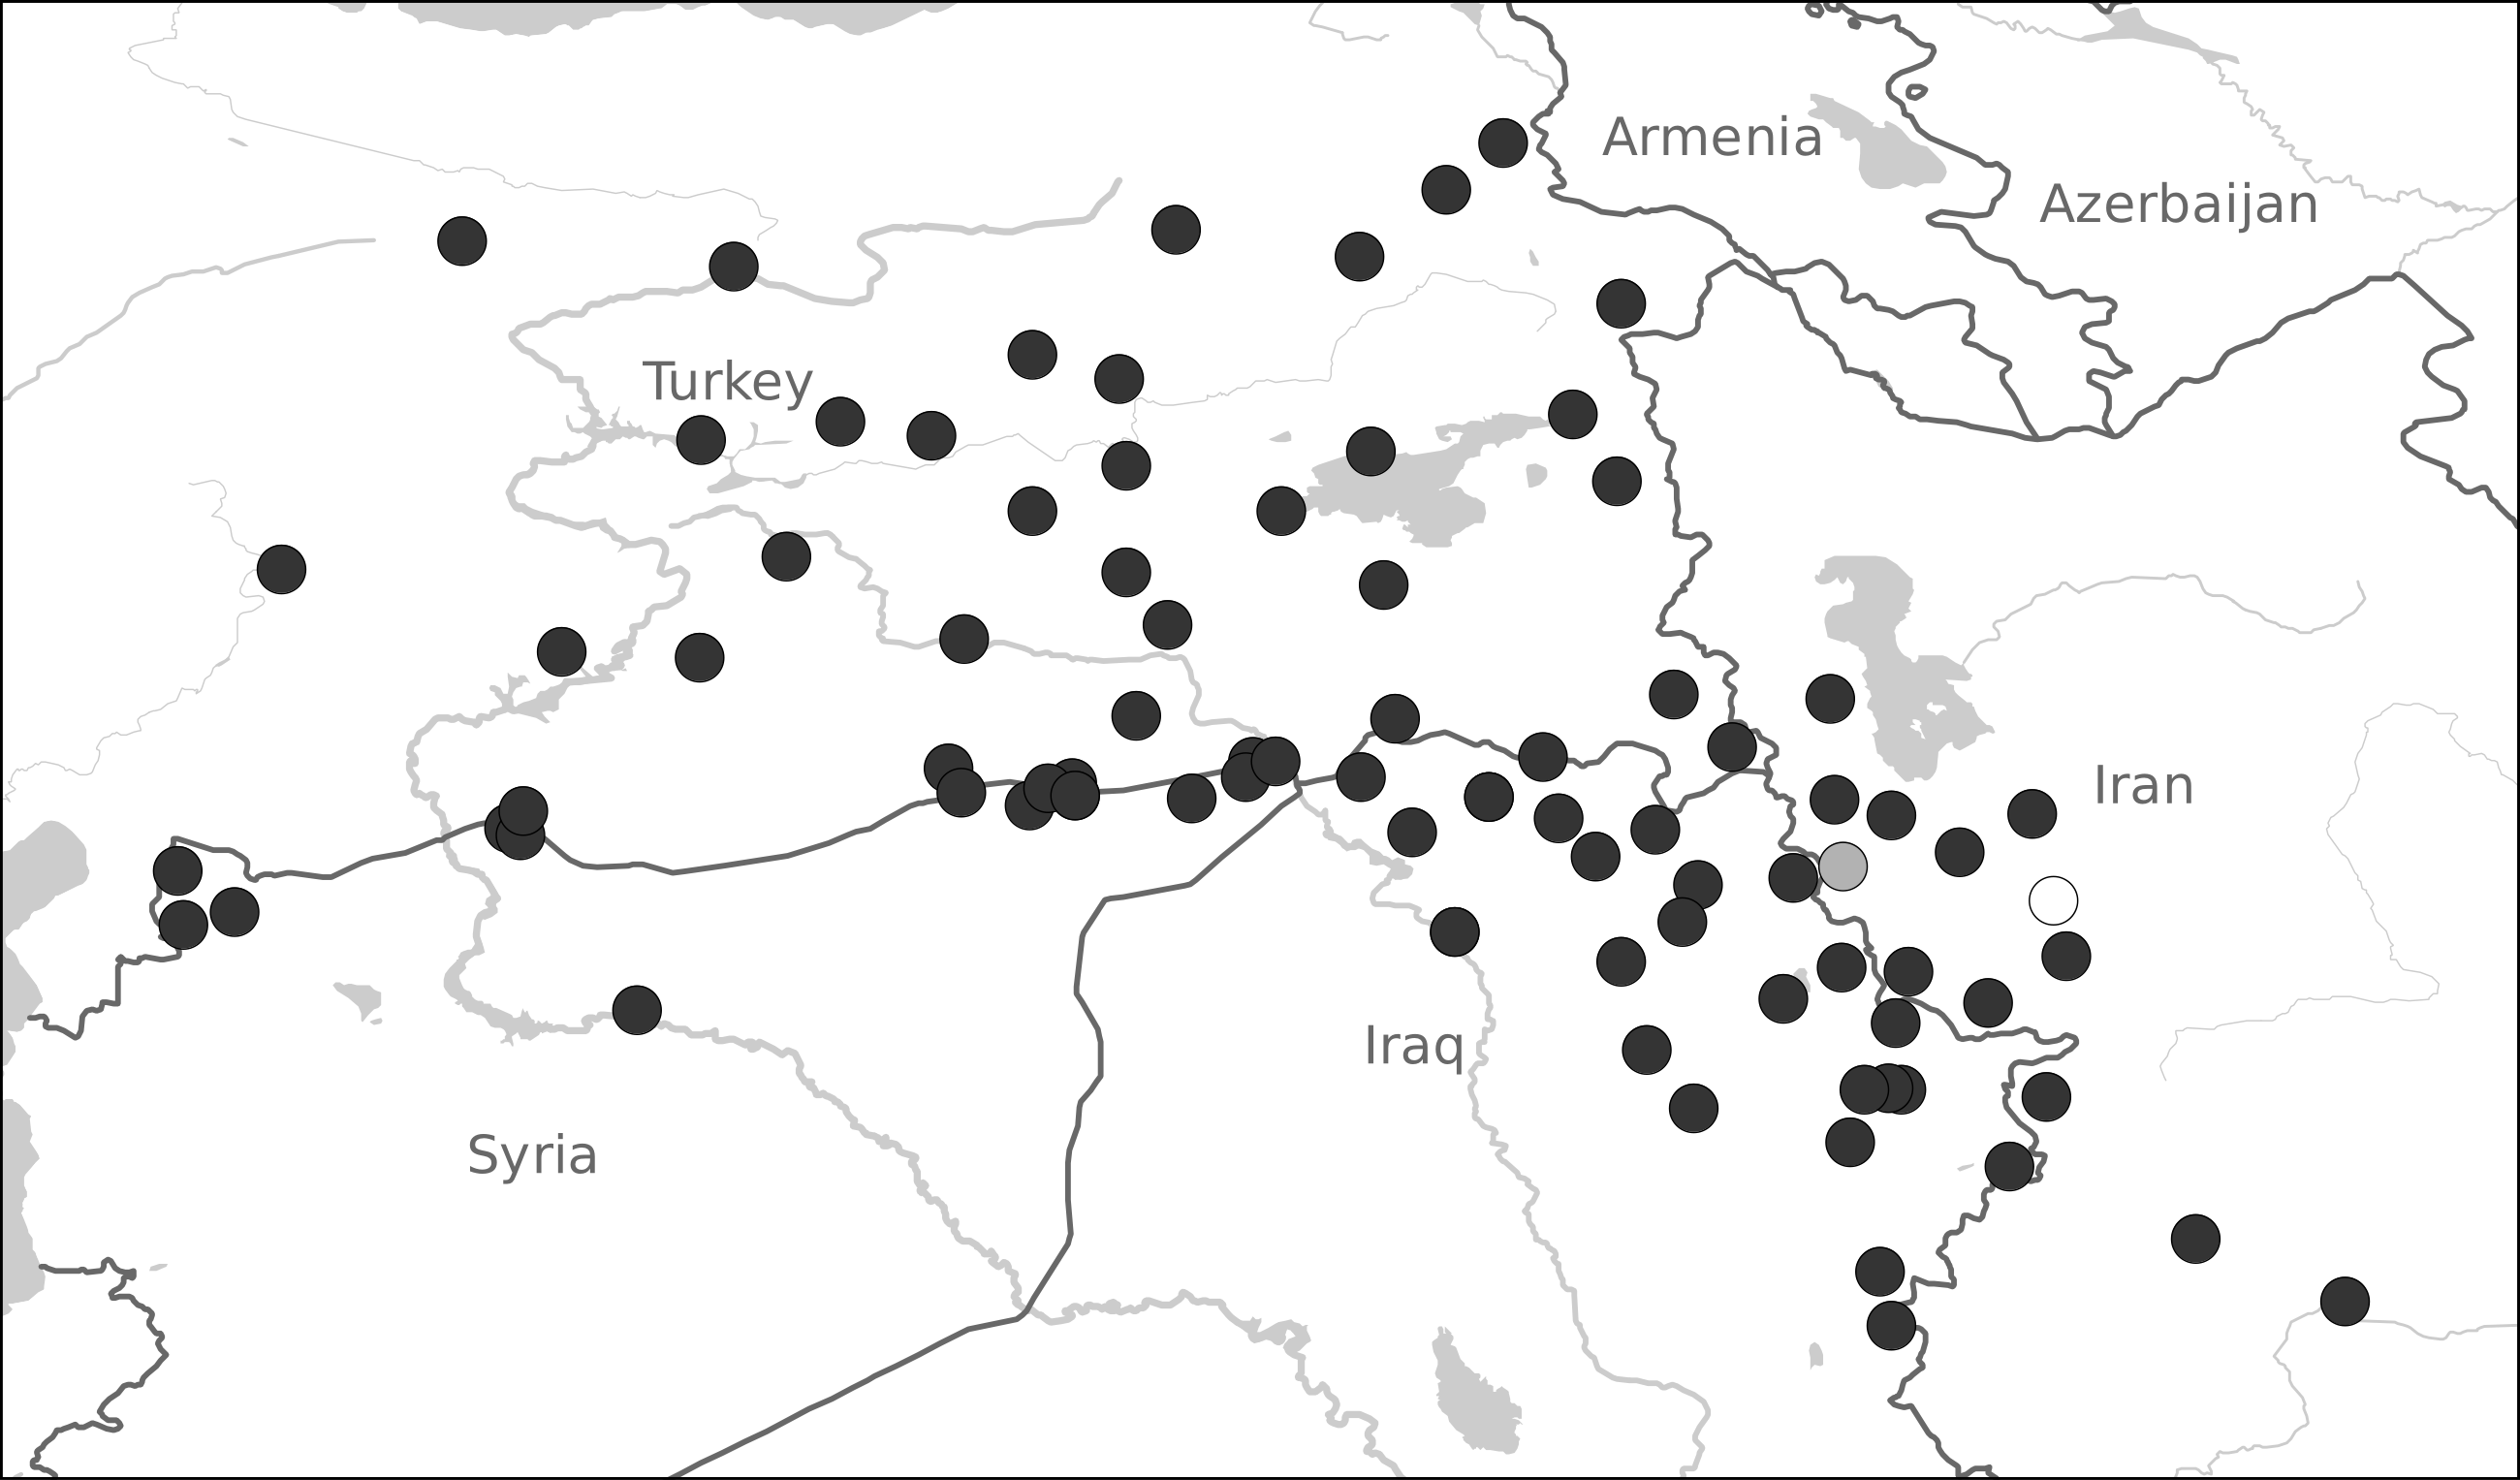
\includegraphics[width=\textwidth]{figures/fig3_map_motion.png}
\caption{\label{fig:key:2}Post-predicate goals of verbs of motion \citep[12]{Haig2022}}
\end{figure}

\begin{figure}
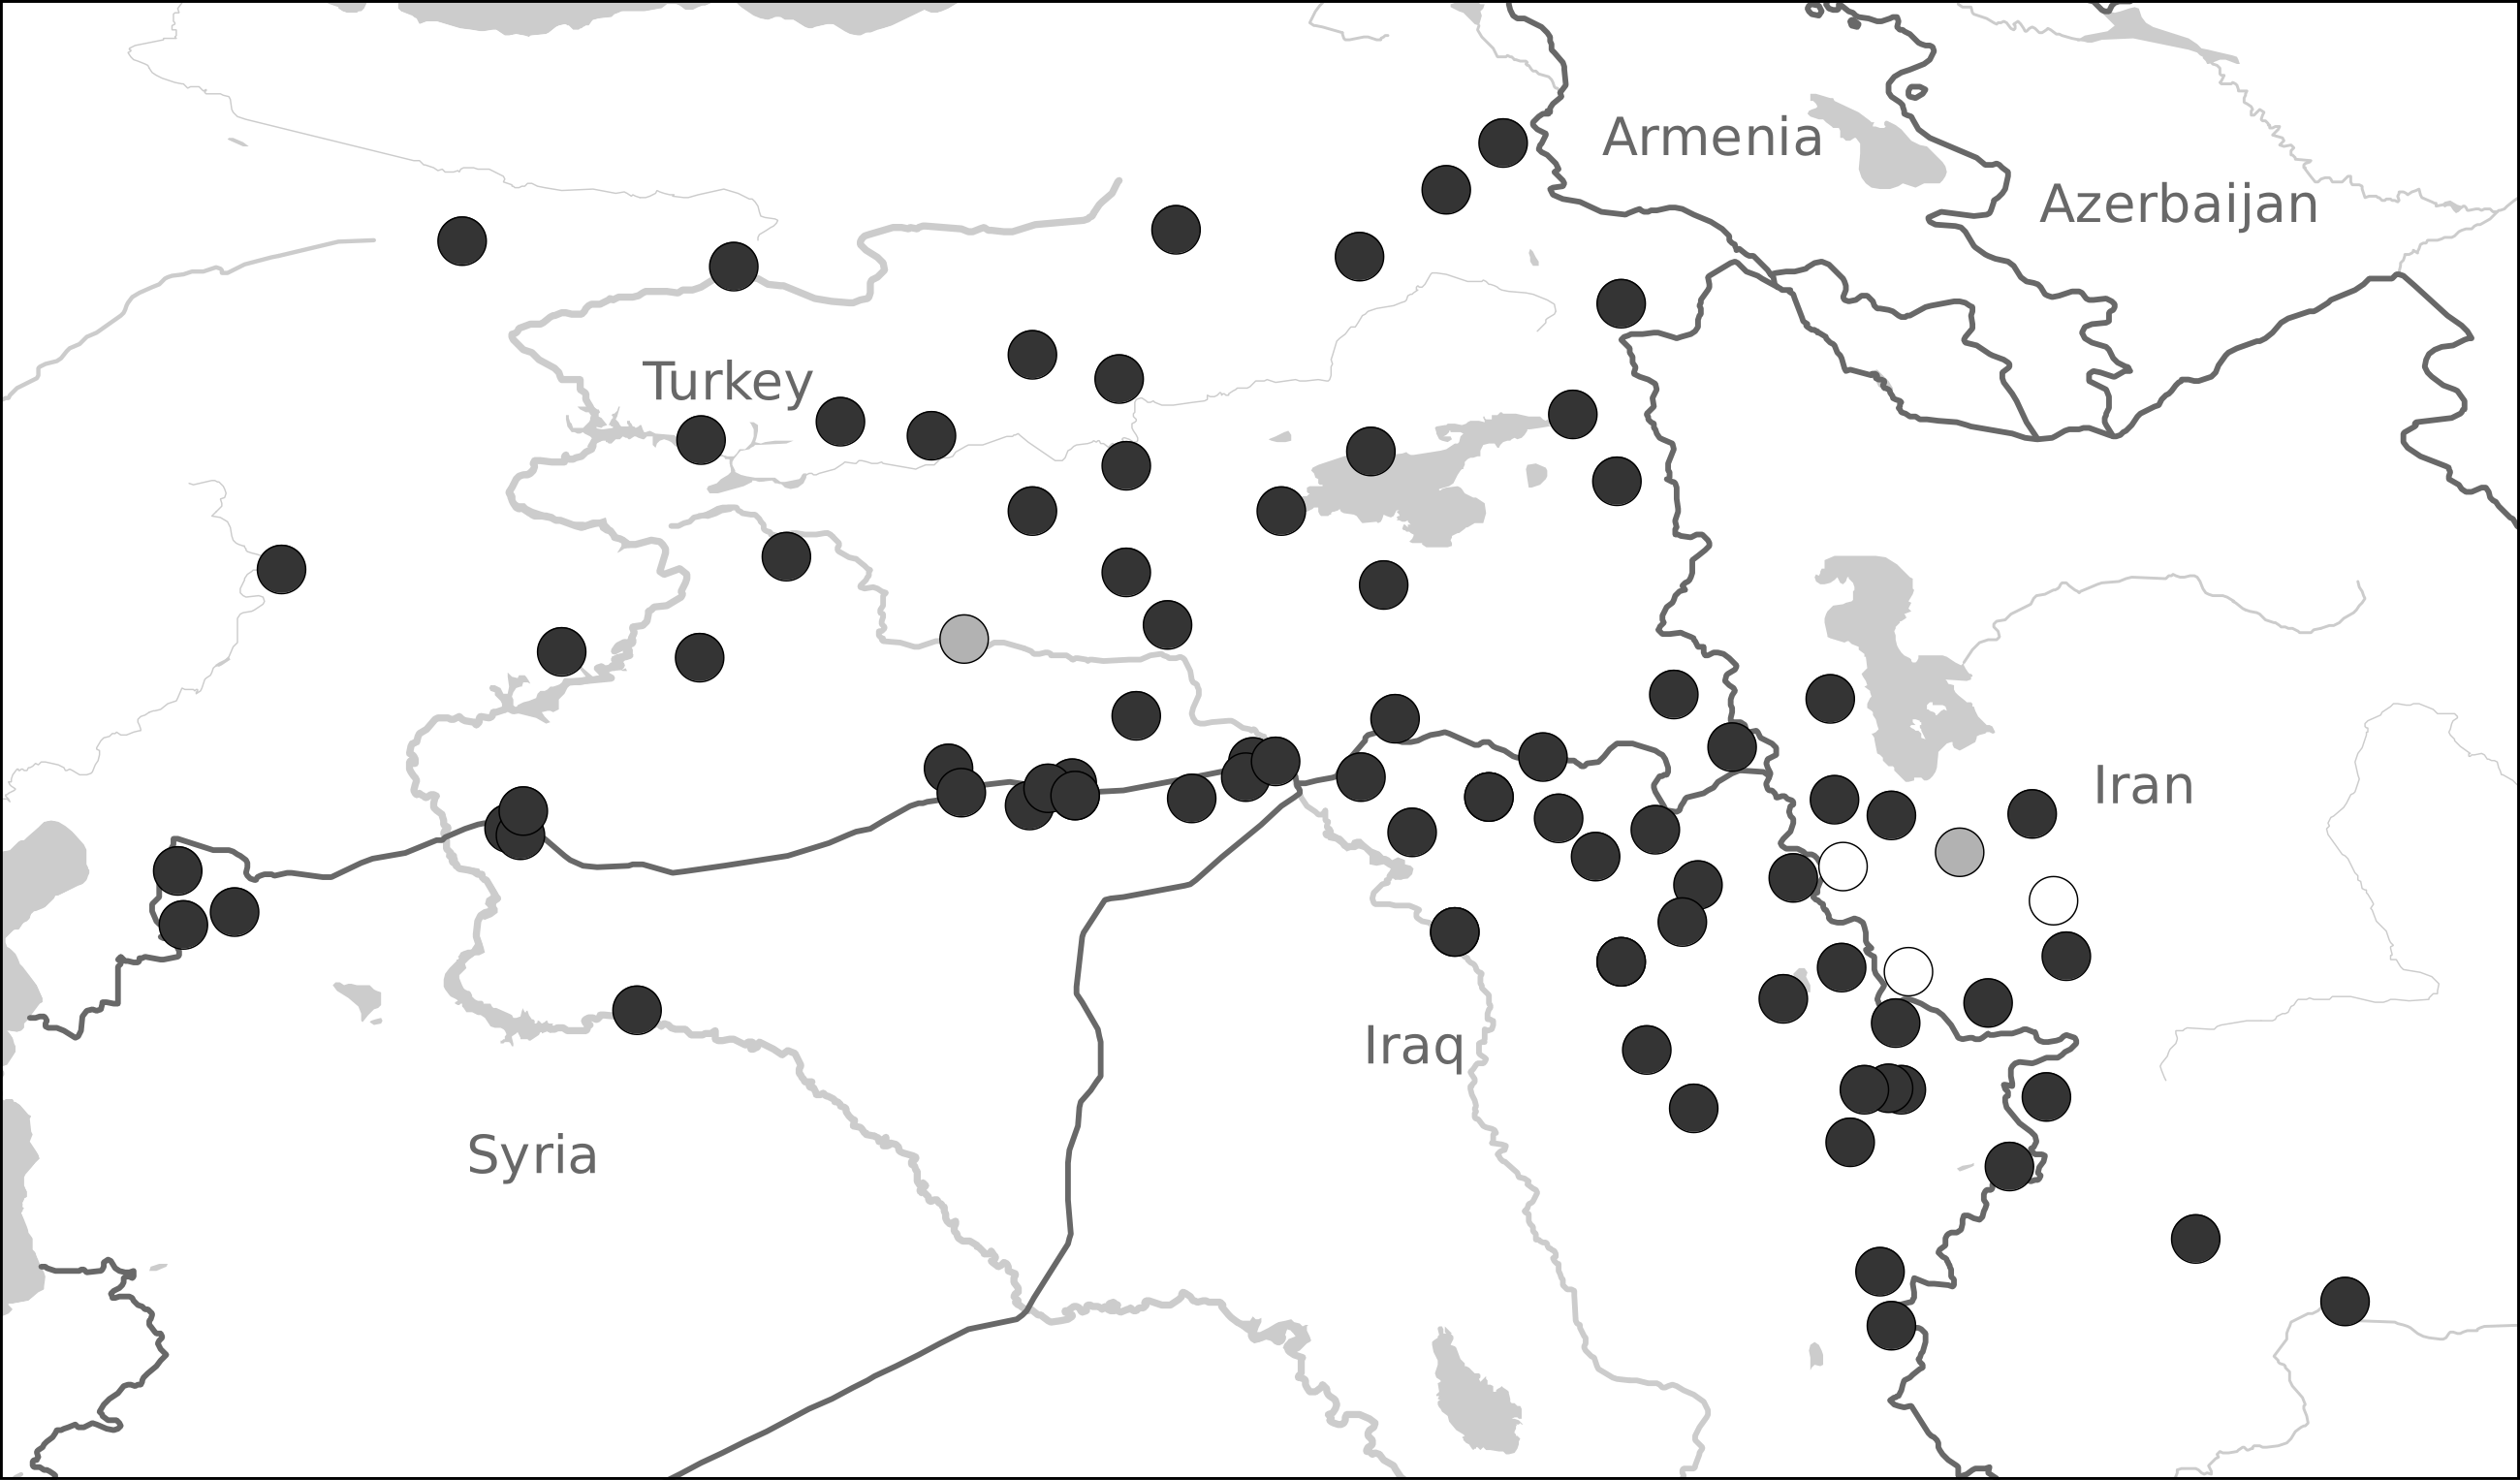
\includegraphics[width=\textwidth]{figures/fig4_map_causedmotion}
\caption{\label{fig:key:3}Post-predicate goals of verbs of caused motion \citep[12]{Haig2022}}
\end{figure}

Figures \ref{fig:key:2} and \ref{fig:key:3} illustrate the distribution of post-predicate goals for verbs of motion and caused motion across different Kurmanji dialects. Black dots indicate that at least 50\% of the goals were placed in the post-predicate position, while gray dots represent an equal number of goals placed in both the post- and pre-predicate positions. White dots indicate that less than 50\% of examples were positioned in the post-predicate position. It is important to note that the data encompass both types of flagging: goals flagged with adpositions as well as those flagged with case. Since case-flagged goals are always positioned post-predicatively, the figures do not provide a clear representation of the distribution of adpositional goals in the pre- and post-predicate positions. Furthermore, Figures \ref{fig:key:2} and \ref{fig:key:3} indicate that goals of motion and goals of caused motion are predominantly placed in the post-predicate position across all Kurmanji dialects. However, there are exceptions in the Kurmanji spoken in Iran, where pre-predicate goals make up the majority and are flagged with a preposition (for a discussion, see \citealt{Haig2022}: 13).

At the same time, \citet{Haig2014} observes that the use of post-predicate adpositional goals is quite limited in various Kurmanji dialects. In the southeastern Anatolian dialects, goals are frequently accompanied by a preposition or a circumposition. In contrast, the central Anatolian dialects do not use adpositions with goals, instead employing bare noun phrases (NPs). The only exception is for human goals, which are marked by the preposition \textit{cem} ‘to,’ as illustrated in example \REF{ex:key:17}.

\ea%17
  \label{ex:key:17} Kurmanji (\citealt{Matras2016}: K092, Sunak Köyü)\\
\gll Otobus     hat-e     cem   me \\
bus    come.\textsc{pst.3sg-drct}      \textsc{adp}    us\\
\glt ‘The bus came to us.’ 
  \z

The next type of goal are recipients of verbs of transfer. \citet{Haig2022} reports only two examples of goals of transfer in the Database of Kurdish Dialects, and both are flagged with case. Hence, the recipient argument in the examples is placed after the predicate.

\ea%18
  \label{ex:key:18} Kurmanji (\citealt{Matras2016}: K010, Tunceli)\\
  \gll Ew  ne-da      min \\
it  \textsc{neg-}give\textsc{.pst.3\textsc{sg}}  me\\
\glt ‘He didn’t give it to me.’ 
  \z

Furthermore, Gündoğdu (2019) notes that the semantics of verbs of transfer influence the flagging and positioning of their arguments. For instance, the verbs \textit{dan} ‘to give’ and \textit{firotin} ‘to sell’ flag their recipients with oblique case, resulting in these recipients being placed in the immediate post-predicate position. In contrast, the verb \textit{şandin} ‘to send’ flags its recipients with an adposition, placing them in the pre-predicate position.

The final type of goal is the addressees of verbs of speech. \figref{fig:key:4} illustrates the distribution of these goals in either the pre- or post-predicate position.

\begin{figure}
% 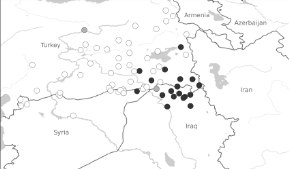
\includegraphics[width=\textwidth]{figures/iefremenko-img004.png}
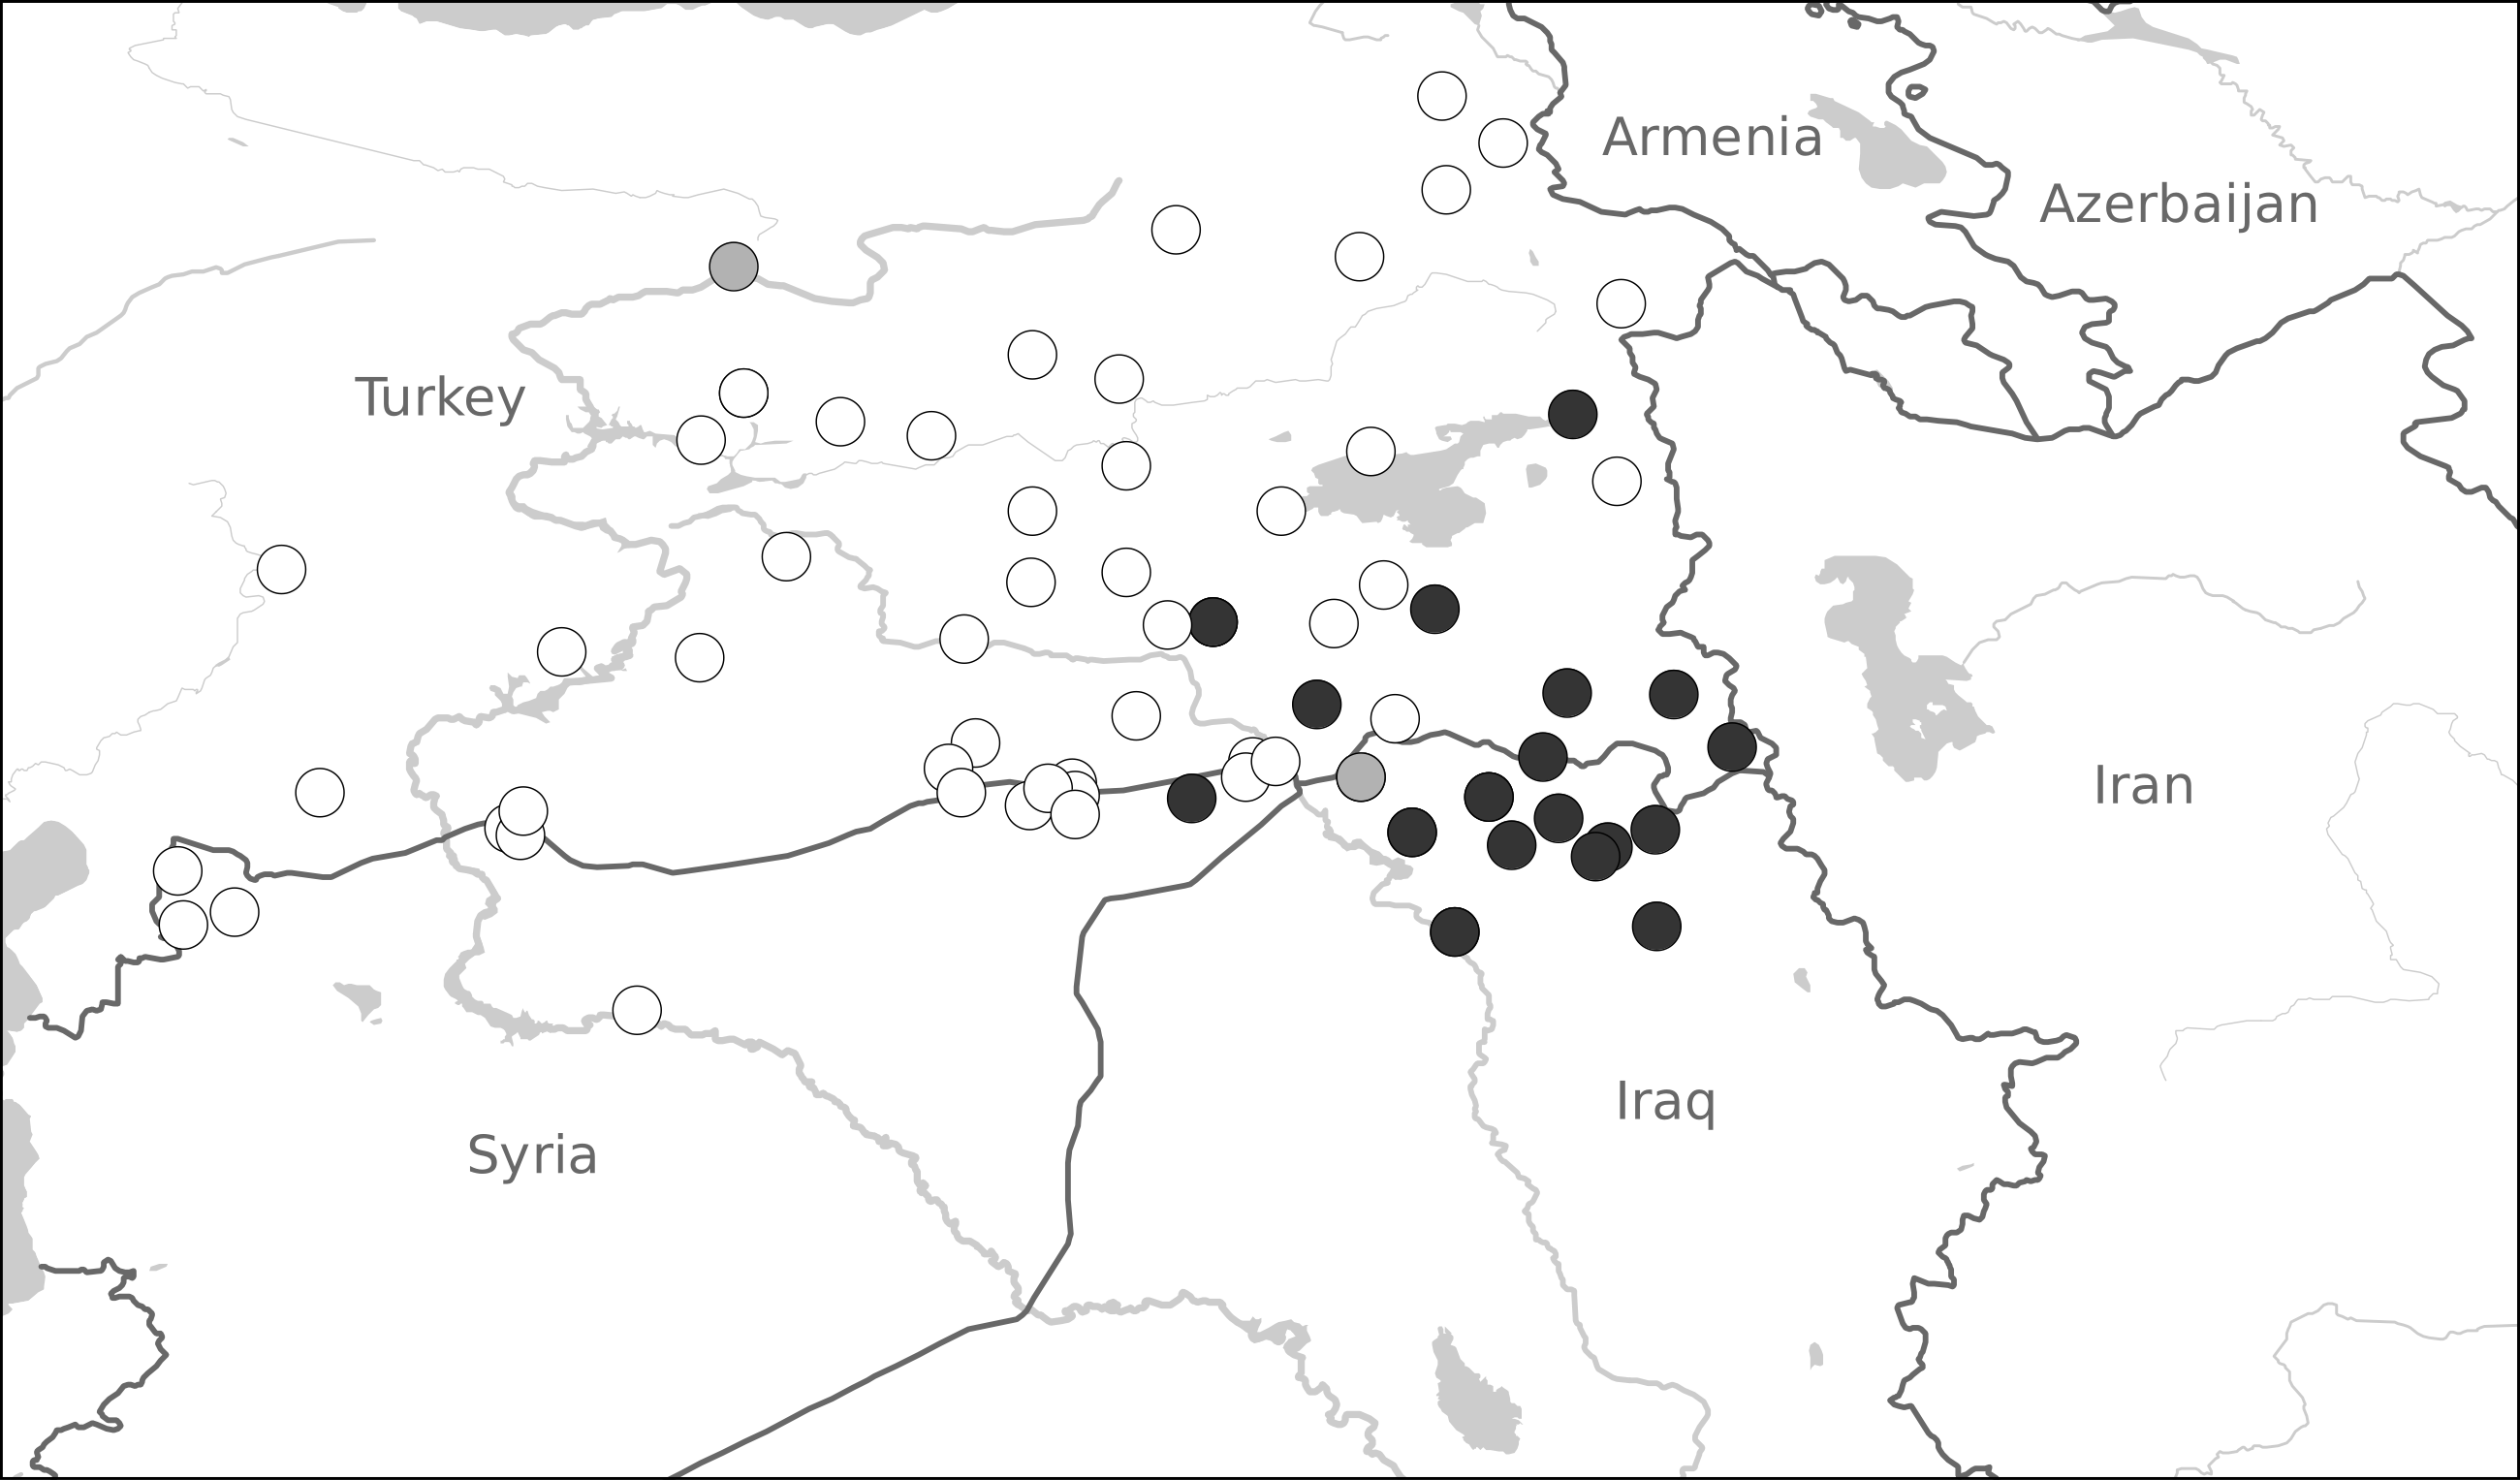
\includegraphics[width=\textwidth]{figures/fig5_map_addressee.png}
\caption{\label{fig:key:4}Post-predicate addressee arguments \citep[15]{Haig2022}.}
\end{figure}

\figref{fig:key:4} illustrates that in Kurmanji, addressees of verbs of speech are predominantly placed in the post-predicate position, particularly in southeastern Turkey and the Van province. In contrast, the northern dialects favor the pre-predicate position for addressees. For example, in Muş, the pre-predicate position for addressees of verbs of speech is a standard practice \citep{Haig2022}. As discussed by \citet{Haig2014}, the pre-predicate position for addressees is common in dialects that have developed circumpositions such as \textit{ji…ra} (e.g., Muş) or the independent postposition \textit{…ra} (e.g., Malatya). Thus, goal arguments introduced with circumpositions and postpositions are consistently placed in the pre-predicate position, while those flagged with prepositions are found in the post-predicate position (\citealt{Gundogdu2019}, \citealt{Haig2022}).

\citet{Haig2014} suggests that the variation observed among Kurmanji dialects can be attributed to language contact. This is particularly relevant given that Kurmanji is spoken in the Western Asian Transition Zone. The region can be understood as a contact zone between large-scale typological patterns, involving both differences in basic word order, namely (S)OV versus (S)VO, and differences in adpositional type, including prepositions, postpositions, and ambipositions (\citealt{HaigKhan2019}, \citealt{HaigEtAl2024}). Specifically, the OVX word order in Kurmanji developed through contact with earlier Semitic and Iranian languages (\citealt{Haig2014}, \citealt{HaigThiele2014}). Additionally, \citet{Haig2020} and \citet{Haignforth} note that in historically (S)OV languages, locational goals, along with recipients and addressees, are the primary candidates to move into the post-predicate position, while preverbal (indefinite) direct objects and copular complements tend to be more stable.

As a result of the aforementioned factors, the southernmost dialects, which have maintained prolonged contact with Neo-Aramaic, tend to place goals, addressees and recipients predominantly after the verb. In contrast, the northern and western dialects have experienced extensive contact with Armenian and Turkish, resulting in a strong preference for the preverbal placement of these constituents. Additionally, southern dialects show a tendency to use prepositions or circumpositions when introducing post-predicate elements. Conversely, in the dialects of Central Anatolia, the combination of a post-predicate consituent with a preposition is highly restricted.

\subsection{The effect of information structure on the use of the post-predicate position}\label{sec:key:3.3.3}

The placement of post-predicate elements in Kurmanji is syntactically fixed and is not affected by pragmatically driven scrambling or stylistic variation, in contrast to Turkish, for instance \citep{Haig2022}. As mentioned at the beginning of \sectref{sec:key:3.3}, this study focuses on Kurmanji as spoken in Turkey and Germany, while also drawing inspiration from research on other Kurdish languages and Persian.

\citet{Asadpour2021} conducted an extensive analysis of word order in goal constructions across various languages spoken in northwestern Iran, including Mukri Kurdish. This analysis examined multiple factors to provide a comprehensive understanding of word order patterns, including semantic factors such as animacy, number, and the semantic class of verbs. The author also investigated morphosyntactic factors, including part of speech, (in)definiteness, and flagging. Additionally, the analysis considered information structure as a discourse-pragmatic factor, along with the syntactic weight of constituents. The results indicated that the semantic class of verbs and flagging are significant predictors of the post-predicate position in Mukri Kurdish, aligning with findings from previous research on Kurmanji. However, Asadpour also demonstrated that information structure plays a crucial role in determining whether goals are placed in the pre- or post-predicate position in Mukri Kurdish. Specifically, it was found that goals in the pre-predicate position are primarily new and given-inactive, while those in the post-predicate position typically represent given or accessible information. This finding has not been previously documented in Kurdish, potentially due to the fact that Asadpour’s study focuses on Mukri Kurdish, which is spoken in northwestern Iran, whereas the studies discussed earlier primarily concentrate on Kurmanji spoken in Turkey. Considering that Kurdish languages are spoken across several countries and come into contact with various languages, the observed variations in these studies may stem from distinctions among the Kurdish languages.

Nevertheless, the current study will explore the influence of information structure on word order in Kurmanji, taking into account the findings from Mukri Kurdish as well as the role of information structure in the word order of Turkish, the contact language.

\subsection{The effect of formality and mode on the use of the post-predicate position} \label{sec:key:3.3.4}

Starting from the second half of the 20th century, efforts have been made to standardize the writing system for Kurmanji, using the Latin alphabet, with the grammar of \citet{KhanLescot1970} being one of the most significant contributions. However, the development of Kurmanji literacy has faced challenges due to social and political factors (\citealt{Derince2013}, \citealt{BrizicnodateEtAl}). In Turkey, Kurmanji speakers often achieve literacy in Turkish, and, in the best-case scenario, become acquainted with the written conventions of Kurmanji only in their adult years (\citealt{HaigMatras2002}). Additionally, Turkish serves as the sole language of governmental and educational institutions, while Kurmanji is primarily used in informal contexts. This lack of familiarity with written language norms of Kurmanji among the Kurmanji-speaking population in Turkey may explain why earlier studies on Kurmanji word order relied on spoken records. Consequently, the impact of mode or formality on word order in Kurmanji has remained largely unexplored.

However, examining Kurmanji's word order across different linguistic registers is important. One reason for this is that previous research on Persian, a language that shares syntactic features with other West Iranian languages, has identified a correlation between formality, mode, and word order. \citet{Frommer1981} found that in Persian, a lower degree of formality corresponds to an increase in post-predicate elements. In other words, while formal written registers are predominantly verb-final, informal spoken registers contain post-predicate elements in more than 70\% of utterances. Furthermore, a recent study by \citet{Haig_post-predicate_EtAl2024-1} supports the findings of \citet{Frommer1981}. By drawing parallels between Persian and Kurmanji, we can hypothesize that similar register effects may exist in Kurmanji, highlighting the need for systematic research on how formality and mode shape word order patterns in Kurmanji.

\section{Studies on the post-predicate position in Kurmanji in language contact situations} \label{sec:key:3.4}

For centuries, Kurds have lived in contact with speakers of various languages, including Persian, Arabic, Turkish, Armenian, and Neo-Aramaic, among others. These interactions have undoubtedly influenced the Kurdish language(s). However, language contact has not been the central focus in Iranian linguistics (\citealt{HaigMatras2002}). Recently, more linguists have begun to investigate the CLI on Kurmanji. Sections \ref{sec:key:2.2} and \ref{sec:key:2.3} provide an overview of several studies conducted in this area.

Contact-induced changes in word order, particularly in the post-predicate position, have attracted increasing interest among scholars in Kurdish linguistics. In addition to the previously mentioned studies (\citealt{Haig2014}, \citealt{Haig2018}, \citealt{Gundogdu2019} \citealt{Haig2022}, \citealt{Asadpour2021}), several other investigations have documented word order variation. For instance, \citet{Dorleijn1996} examined Kurmanji spoken in Diyarbakır, revealing that this dialect exhibits greater syntactic flexibility compared to other Kurmanji dialects. Specifically, speakers demonstrated a preference for using circumpositions to flag goals rather than relying solely on the oblique case. As a result, the placement of goals was not strictly limited to the post-predicate position. Furthermore, \citet{Mahalingappa2009} investigated the acquisition of ergativity in Kurmanji among children living in Kurdish villages near Erzurum. The findings revealed that these children predominantly adhered to the SOV word order pattern. Interestingly, while their parents also primarily produced SOV utterances, there were occasional instances in which subjects were positioned after the verb to emphasize their role, resulting in an OVS word order. In addition, \citet{Kirgiz2022} conducted a study on the acquisition of Kurmanji in bilingual children in Germany. Similar to Mahalingappa's findings, Kırgız found that the children predominantly followed a verb-final word order while placing case-flagged goals in the post-predicate position. Notably, some children also placed subjects in the post-predicate position, indicating a degree of flexibility in their use of word order. Finally, a study by \citet{Herkenrath2021} examines the use of post-predicate elements in three languages in contact: Kurmanji, Turkish, and German. The data were collected from monolingual, bilingual, and multilingual speakers who immigrated to Germany at different ages. The motivations for employing the post-predicate position vary across the three languages: predicate semantics in Kurmanji, information structure in Turkish, and syntactic structure in German. \citet{Herkenrath2021} notes that, in the language contact situations, the reasons for using the post-predicate position overlap among the languages, reflecting their mutual influence on one another. This exploratory study underscores the need for more in-depth investigations into the ongoing changes within these languages.

Studies on Kurmanji in contact situations show that while the language predominantly follows an SOV pattern, there is certain flexibility in the post-predicate position. Both child and adult speakers sometimes place subjects or other constituents after the verb for emphasis or pragmatic reasons. Contact with other languages, such as Turkish and German, further influences the use of post-predicate elements. However, existing studies are still limited in scope, and more systematic research is needed to fully understand how language contact shape word order in Kurmanji.

\section{Word order in German}\label{sec:key:3.5}

The basic word order in German is (S)OV with V2 features (\citealt{Fourquet1977}, \citealt{Bach1962}, \citealt{Bierwisch1966}, as stated in \citealt{kiss_41_2015}). SOV is typically exhibited in embedded and main clauses with periphrastic verb constructions. At the same time, the V2-constraint often leads to SVO or XVS orders in main clauses, as the finite verb is required to occupy the second position in the clause (\citealt{Czinglar2013, Czinglar2014}).

Given the various word order patterns in German, scholars have different opinions on the basic word order of German. Previous research suggests that the base word order in German is SOV. \citet{Muller2023} argues that the assumption of verb-final order as the base order is supported by several observations. For instance, in subordinate clauses introduced by conjunctions, the verb consistently appears in the final position, and verbs tend to cluster at the end of the sentence, as illustrated in example \REF{ex:key:19} below.

\ea%19
  \label{ex:key:19} German (\citealt{Muller2023}: 8) \\
\gll dass  er  ihn  gesehen  haben  muss \\
that  he  him  seen    have  must\\
\glt ‘that he must have seen him’ 
  \z

Secondly, verb particles form a close unit with the verb, and such units can be seen only in verb-final structures, as shown in the example \REF{ex:key:20a}. Consequently, this structure reflects the base order.

\ea \label{ex:key:20} German (\citealt{Muller2023}: 6) \\
\ea\label{ex:key:20a}
\gll weil    er  morgen  an-fängt\\
because  he  tomorrow  \textsc{prt}-start\\
\glt ‘Because he is starting tomorrow’
\ex\label{ex:key:20b}
\gll Er   fängt   morgen   an.\\
He  starts  tomorrow  \textsc{prt}\\
\glt   ‘He starts tomorrow.’ 
\z
\z

Furthermore, certain constructions allow only for (S)OV word order, such as verbs derived from nouns by back-formation (e.g., \textit{uraufführen} ‘to perform something for the first time’). As demonstrated in the examples \REF{ex:key:21} below, there is only one possible position for the verb.

\ea\label{ex:key:21} German (\citealt{Muller2023}: 137) \\
\ea[]{\label{ex:key:21a}
\gll weil     sie   das   Stück  heute  urauf-führen\\
because   they  the   play  today  \textsc{prt-}lead\\
\glt ‘because they are performing the play for the first time today.’
}
\ex[*]{\label{ex:key:21b}
\gll Sie  urauf-führen  heute  das   Stück.  \\
 they  \textsc{prt-}lead  today  the  play\\
 }
\ex[*]{\label{ex:key:21c}
\gll Sie  führen  heute  das  Stück  urauf.\\
they  lead  today  the  play  \textsc{prt} \\
}
\z
\z

Another example of the constructions that allow only SOV word order are verbs used together with the construction \textit{mehr als} ‘more than’ (see examples \REF{ex:key:22} below).

\ea \label{ex:key:22} German (\citealt{Muller2023}: 138) \\
\ea[]{\label{ex:key:22a}
\gll dass   Hans  seinen  Profit  letztes  Jahr  mehr  als  verdreifachte\\
that  Hans  his  profit  last  year  more  than  tripled\\
\glt ‘that Hans increased his profit last year by a factor greater than three.’
}
\ex[]{\label{ex:key:22b}
\gll Hans  hat   seinen   Profit   letztes   Jahr   mehr   als   verdreifact\\
Hans   has   his   profit   last   year   more   than   tripled\\
}
\glt ‘Hans increased his profit last year by a factor greater than three.’
\ex[*]{\label{ex:key:22c}
\gll Hans  verdreifachte  seinen Profit  letztes  Jahr  mehr  als\\
Hans  tripled    his  profit  last  year  more  than\\
}
\z
\z

Additional evidence for the base word order in German being (S)OV comes from the studies on the L1 acquisition of German that show that children start acquiring the word order with (S)OV structures (\citealt{ClahsenMuysken1986}, \citealt{Jordens1988}, \citealt{SchulzEtAl2008}, \citealt{TracyThoma2009}).

On the other hand, German is also characterized as a verb-second (V2) language. In German, V2 appears in main declarative clauses with a finite main verb, as shown in example \REF{ex:key:23}, and in wh-questions (\textit{W-Fragen}), as demonstrated in \REF{ex:key:24}. As for main declarative sentences with V2, any constituent can be placed before the finite verb \citep{Muller2023}, but importantly, only one constituent can be placed before the verb in the V2 word order \citep{Czinglar2013}. Although analyses of corpora of the spoken and written German language show that only half of the main sentences begin with a subject (\citealt{HinrichsKübler2005}, as cited in \citealt{Czinglar2013}), the existence of examples such as \REF{ex:key:23} and \REF{ex:key:24} has led some researchers to analyze German word order as SVO in main sentences and SOV in embedded clauses (for example, \citealt{Bohn1983}, as stated in \citealt{Vikner2019}) or as lacking a dominant word order altogether \citealt{wals-81}.

 \ea 
    \label{ex:key:23} German, self-constructed \\
 \gll Anna  schreibt  ihrem  Bruder    einen  Brief.\\
  Anna  writes    her  brother    a  letter\\
\glt ‘Anna is writing her a letter to her brother.’ 
\z

\ea%24
  \label{ex:key:24} German, self-constructed \\
\gll Was   schreibt Anna   ihrem   Bruder? \\
what  writes   Anna  her  brother\\
\glt ‘What is Anna writing to her brother?’ 
  \z

A widely used descriptive representation of German clause structure is provided by the Topological Model (\citealt{Drach1937}, \citealt{WollsteinEtAl2006}, \citealt{Wollstein-leisten2014, Wollstein2018}). As illustrated in \figref{fig:key:5}, finite and non-finite verbs together form a sentence bracket, which is positioned after the prefield and encompasses the middle field.


\begin{figure} 
\begin{tabular}{ccccc}
 & \multicolumn{3}{c}{$\overbrace{\hspace{7cm}}^{\text{\normalsize Sentence brackets}}$} & \\
Prefield & Left Bracket & Middle Field & Right Bracket & Postfield \\
\end{tabular}
\caption{\label{fig:key:5}Illustration of the Topological Model}
\end{figure}

In main clauses, the left bracket contains the finite verb, while the right bracket accommodates the infinite verb. The prefield allows for the fronting of any constituent, determined by discourse context and information structure, but the V2 constraint limits it to just one constituent. Furthermore, German can also place elements after the right bracket, and this construction is commonly referred to as \textit{Nachfeld} ‘post-field’ (\citealt{Frey2015}, \citealt{Hartmann2017}). The post-field is typically considered an area that holds heavy constituents, such as subordinate clauses or other constituents extraposed from the middle-field in order to reduce cognitive load (\citealt{Imo2015}, \citealt{Proske2015}). \tabref{tab:key:3.1} exemplifies the Topological Model for the German clause ‘(Yesterday we realized that) Maria (had) sent the child a letter from Berlin.’

\largerpage[3]
\begin{table}[b]\small
\begin{tabularx}{.95\textwidth}{llXlXlX}
\lsptoprule
\textbf{Prefield}  & \textbf{Left} & \textbf{Middle Field}  & \textbf{Right} & \textbf{Post-field}\\
& \textbf{Bracket} &  & \textbf{Bracket} & \\
\midrule
\textit{Maria} & \textit{schickte} & \textit{dem Kind einen Brief aus Berlin.} & &\\
Maria & sent & the child a letter from Berlin. &  & \\
\midrule
\textit{Maria} & \textit{hat} & \textit{dem Kind einen Brief} & \textit{geschickt} & \textit{aus Berlin.}\\
Maria & has & the child a letter & sent & from Berlin. \\
\midrule
\textit{Wir} & \textit{haben} & \textit{gestern} & \textit{festgestellt,} & \textit{dass Maria dem Kind einen Brief geschickt hat.} \\
We & have & yesterday & found out & that Maria had sent the child a letter from Berlin. &  \\
\lspbottomrule
\end{tabularx}
\caption{\label{tab:key:3.1} The Topological Model for German.}
\end{table}

As demonstrated in \tabref{tab:key:3.1}, the post-field can contain clausal (e.g., \textit{dass Maria dem Kind einen Brief geschickt hat} ‘that Maria had sent the child a letter’) or non-clausal constituents (\textit{aus Berlin} ‘from Berlin’). However, since the focus of this study lies in the non-clausal constituents positioned after the predicate, attention will be directed to them.

There are several types of non-clausal constituents placed in the post-field in German. Below are examples of such constituents, where \REF{ex:key:25} demonstrates an extraposed prepositional phrase, \REF{ex:key:26} shows an extraposed determiner phrase, \REF{ex:key:A} and \REF{ex:key:B} present an adverbial and an adjectival phrase respectively, and \REF{ex:key:C} is an example of a discourse marker in the post-field. Constituents that belong to the post-field in the examples (25-29) are in italics.

\ea%25
  \label{ex:key:25} German, (\citealt{Hartmann2017}: 101)\\
\gll Jeder    möge    seiner    Steuererklärung  ein Protestschreiben  beifügen,  \textit{mit} \textit{folgendem} \textit{Inhalt:} … \\
everybody  should    his    tax\_declaration  a protest\_letter    add    with  following  content …\\
\glt ‘Everybody should add a protest letter to his tax declaration with the following content.’ 
  \z

\ea%26
  \label{ex:key:26} German (\citealt{AkanHartmann2019}: 125)\\
\gll Auf  Gleis    eins  fährt  ein:  \textit{die} \textit{verspätete} \textit{Regionalbahn} \textit{nach} \textit{Wiesbaden.}\\
on  platform  one  arrives  \textsc{prt}  the  delayed  regional\_train to  Wiesbaden\\
\glt ‘The delayed train to Wiesbaden is arriving on platform one.’ 
  \z

Importantly, \citet{AkanHartmann2019} note that German allows only structurally complex determiner phrases in the post-predicate position, as in example \REF{ex:key:26}.

\ea%27
  \label{ex:key:A} German (\citealt{Frey2015}: 67)\\
\gll Wann  hat  Otto  gesprochen  mit  so  viel  Leidenschaft?  \\
  when  has  Otto  spoken    with  so  much  passion\\

  \gll Otto  hat  gesprochen  mit  so  viel  Leidenschaft  \textit{am} \textit{Montag}\\
Otto  has  spoken    with  so  much  passion  on  Monday\\
\glt --- ‘When did Otto speak with so much passion?’\\
     --- ‘Otto spoken with so much passion on Monday.’  \\
  \z
\newpage
\ea%28
  \label{ex:key:B} German, self-constructed\\
\gll Der  Kuchen  war  köstlich,  den  meine    Oma   gebacken  hat,  \textit{frisch} \textit{aus} \textit{dem} \textit{Ofen.}\\
 the  cake    was  delicious,  that  my    grandmother baked    has,  fresh  from  the  oven\\
\glt ‘The cake was delicious, which my grandmother baked, fresh out of the oven.’ 
  \z

\ea%29
  \label{ex:key:C} German (\citealt{Tsehaye2023}: 7) \\
\gll und   die  Autofahrer sind   dann   auch   gleich     ausgestiegen. \textit{und} \textit{so}\\
and  the drivers    are  then  also  immediately  exited    and  so on\\
\glt ‘And the drivers immediately exited and so on.’
  \z

Although the post-field has not received significant attention from researchers, some studies have investigated the use of constituents in the post-field. For instance, \citet{Proske2010}, as cited in \citet{Hartmann2017}, found that approximately one-third of the sentences in her data contain elements in the post-field, with 72\% of these instances being embedded clausal constituents. The remaining non-clausal elements in the post-field include prepositional phrases at 44\%, determiner phrases at 33\%, adverbials at 17\%, and adjectives at 6\%.

Furthermore, a recent study by \citet{Tsehaye2023} investigates the use of non-clausal constituents among monolingual adolescent German speakers in Germany and heritage speakers of German in the US, using data collected through the same methodology as that used in the current study. The findings indicate that 19.08\% of all utterances from monolingual speakers contained a non-clausal constituent in the post-field. Of these, 9.84\% were prepositional phrases, 5.02\% were discourse markers 2.01\% were adverbial phrases, 1.81\% were determiner phrases, and 0.4\% were adjectival phrases. Additionally, the study emphasizes that formality and mode significantly affect the production of non-clausal constituents in the post-field: speakers produced notably more post-field constituents in informal settings compared to formal ones, as well as in spoken mode rather than in written mode.

\largerpage
Other studies emphasize the impact of mode and formality on the use of the post-field in German. For example, \citegen{Engel1974} findings, as cited in \citet{Erdal1999}, indicate that extraposed elements occur five times more frequently in spoken data compared to written data. Similarly, \citet{Proske2015} notes that certain syntactic categories, such as specific adverbs and modal particles, appear in spoken language but are not acceptable in written texts. Conversely, \citet{Imo2015} does not address unacceptability but rather discusses different preferences for post-predicate constituents in spoken and written modes. Imo's research examines the occurrence of non-clausal constituents in the \textit{Nachfeld} in informal spoken and written settings. The findings reveal that the most common constituents in the \textit{Nachfeld} of spoken language are locative and temporal adverbs. However, the use of locative adverbs cannot be generalized as typical for the \textit{Nachfeld} in informal written German, instead, the temporal adverb \textit{heute} ‘today’ and various \textit{irgend}- ‘some-’ adverbs frequently appear. In addition to mode, formality also influences the use of the post-field in German. Previous research has documented significant variation in the frequency of post-field occurrences in written language, with the fewest instances found in scientific texts and the highest occurrences in informal productions (\citealt{Roelcke1997}, as cited in \citealt{Tsehaye2023}).

\section{Summary} \label{sec:key:3.6}

In summary, the word order in the three languages under investigation is SOV. However, each language employs the post-predicate position to different extents, influenced by different factors. Specifically, this position is determined by information structure in Turkish, predicate semantics in Kurmanji, and syntactic structure in German.

Despite these differences, there are also overlaps in the factors influencing the use of the post-predicate position. For example, \citet{Asadpour2021} suggests that, in addition to predicate semantics, information structure also affects the use of the post-predicate position in Kurdish, however, the data for this study are based on Mukri Kurdish spoken in Iran. If information structure similarly influences the word order of Kurmanji spoken in Turkey, it would indicate a shared factor—information structure—that affects both Kurmanji and Turkish in employing the post-predicate position.

Moreover, common factors influencing the use of the post-predicate position in Turkish and German include mode and formality: the post-predicate position tends to occur more frequently in spoken language compared to written language and in informal settings compared to formal ones. While the effects of formality and mode on word order in Kurmanji have not been thoroughly documented, some studies suggest these factors are relevant in Persian, a language that shares syntactic features with other West Iranian languages (\citealt{Frommer1981}, \citealt{Haig_post-predicate_EtAl2024-1}). The potential influence of formality and mode on the use of post-predicate constituents further emphasizes the importance of considering register as a factor in this analysis.

Ultimately, the combination of similarities and differences in the factors influencing the post-predicate position across Turkish, Kurmanji, and German makes this topic particularly intriguing for examination.


\chapter{Methodology}\label{chap:key:4}
\section{The ``Language Situations'' method }\label{sec:key:4.1}

The method used for data collection for this study is called ``Language Situations'', developed by \citet{Wiese2020} and later refined by members of the ‘Research Unit Emerging Grammars’ (RUEG). This method was developed to capture actual language use while simultaneously maintaining sufficient control over participants' productions to gather comparable data relevant to specific research questions. In doing so, it combines the benefits of controlled elicitation with those of natural data collection. Furthermore, it captures language productions across different communicative situations, allowing comparisons across informal and formal settings and spoken and written modes.

\largerpage
The stimulus is a short (one-minute) video clip depicting a staged car accident. After watching it, participants were asked to imagine that they had witnessed this accident. Their task was to describe what they had seen in four different communicative situations: to their close friend via a WhatsApp voice message (informal spoken) and a WhatsApp text message (informal written), to report the accident to the police via a voice recorder (formal spoken) and to write a witness report to the police (formal written). These situations were labelled as formal and informal for the purposes of the study. At the same time, formal and informal communication should not be understood as fixed or homogeneous categories, as they can be realized in a range of different communicative situations. In the present design, situational variation was therefore operationalized specifically through the addressee, the medium of communication, and the spoken versus written mode. For ease of reference, the labels formal spoken, formal written, informal spoken, and informal written are used throughout the manuscript.

\begin{figure}
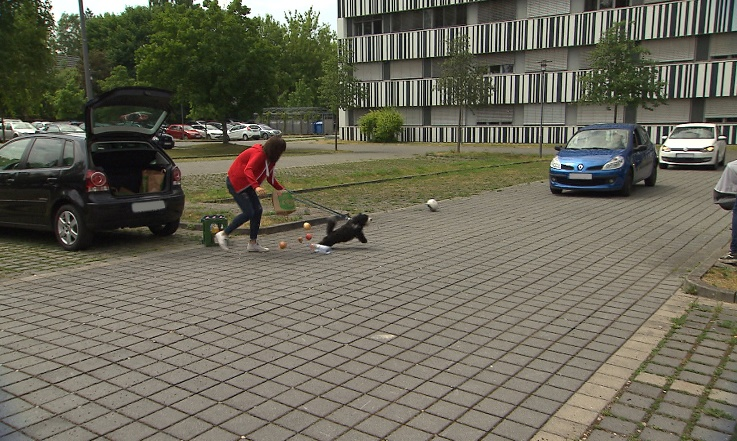
\includegraphics[width=\textwidth]{figures/iefremenko-img005.jpg}
\caption{\label{fig:key:4.1}A screenshot from the video stimulus.}
\end{figure}

There was a break of approximately 10--15 minutes between the informal and formal elicitations. Bilingual participants completed the task in both languages, heritage and majority\footnote{As shown in Section 2.3, Kurmanji speakers have been reported to experience language anxiety when using Turkish, primarily based on adolescent populations (see \citealt{Sahin-firat2010}). In the present study, however, which includes adult participants, no overt anxiety or resistance to speaking Turkish was observed. All participants lived in Ankara and used Turkish in their daily lives.}, while trilingual speakers in Germany did it in their heritage languages, Kurmanji and Turkish.\footnote{German was not collected for the trilingual participants because the aim of the study was to focus specifically on the trilingual speakers’ heritage languages.} There was a break of at least three days, but typically a week, between the sessions. It is also important to note that in informal situations, the elicitor instructed participants to imagine that they were talking to a friend with whom they usually spoke in the tested language. To prevent potential priming effects, the order of the communicative situations and languages was balanced. Depending on the number of participants in each group, at least one, and in most cases two, participants were assigned to each order (heritage vs. majority, formal vs. informal, spoken vs. written). The table with the orders can be found here: https://osf.io/m82qe.

To obtain data that reflected natural language use in both informal and formal contexts, it was essential to create a realistic environment. As the experiment was conducted mostly in universities, schools, or offices, establishing a formal atmosphere was relatively straightforward. Typically, the setting consisted of a classroom furnished with a table and two chairs. The table held only a laptop, a voice recording device, and consent forms. A formally dressed elicitor conducted the session, interacting with participants using formal language, explaining the elicitation procedure, and requesting signatures on the consent forms. Creating a comfortable and relaxed informal setting proved more challenging. For this purpose, a smaller, well-lit room decorated with colorful rugs, flowers, and a tablecloth was chosen. Refreshments such as cookies, tea, and coffee were provided. A different elicitor, dressed casually, engaged participants in friendly conversation. Each participant first spent 12--15 minutes chatting with this informal elicitor about topics such as free time, hobbies, favorite music, books, and movies. These measures aimed to foster a welcoming atmosphere and help participants feel as comfortable and relaxed as possible.

Data collection took place between October 2018 and February 2020. All participants signed a written consent form that clarified data protection issues in accordance with the General Data Protection Regulation (GDPR) of the European Union. The study received approval from the ethics committee of the German Linguistics Society (\textit{Ethikkommission der Deutschen Gesellschaft für Sprachwissenschaft}). The entire elicitation process was recorded using a Tascam DR-05X voice recorder. A black Fujitsu laptop with a 15.6-inch screen was used to display videos and facilitate the writing of formal texts. For written productions, participants typed a WhatsApp text message using an iPhone 6 and a witness report on the laptop, where they could choose from various keyboards depending on the language. Participants in Germany had the option to use either a German keyboard or an external Turkish keyboard. Additionally, Kurmanji participants were informed where to find diacritics for some of the Kurmanji letters.

Collecting metalinguistic data from participants involved using a comprehensive questionnaire inspired by the one developed in the MULTILIT project \citep{SchroederEtAl2015} and further refined by the RUEG project team. The questionnaire consisted of ten sections, covering administration, general participant information, educational background, language proficiency, family background, self-assessment of language skills, language use with family members and peers, media consumption and leisure activities, personal character traits, and feedback on their participation in the study. It was available in both German and Turkish, allowing participants to complete it in the majority language of the country they reside in. Participants always filled out the questionnaire in the presence of an elicitor.

Several limitations should be considered when employing the 'Language Situations' method. Firstly, despite the natural context, many speakers may encounter situations, such as reporting an accident to the police, in their heritage language for the first time. For example, in Turkey, Kurmanji is not used in formal public settings, and interactions with governmental institutions typically occur in Turkish. However, even if participants lack experience in reporting accidents to the police in their heritage language, they are likely to possess knowledge of formal registers in the dominant language of their country, which is usually acquired through education. Therefore, one of the rationales for eliciting witness reports in participants’ heritage language is to capture their innovative strategies for using structures characteristic of formal language, drawing upon their understanding of language registers.

Furthermore, this method has limitations regarding the analysis of information structure. It was designed so that each speaker retold the accident four times across different communicative situations. Additionally, bilingual participants were asked to do the same in both of their languages, with a minimum break of three days between sessions. This means that bilingual participants narrated the same story a total of eight times, while monolingual participants retold it four times.

More information about the method, including consent forms, data collection instructions, questionnaires in PDF format, and elicitation orders, is publicly available in the Open Science Framework (OSF) repository at https://osf.io/qhupg/.

\section{Participants}\label{sec:key:4.2}

The study involved four groups of participants: heritage speakers of Turkish in Germany, heritage speakers of Kurmanji and Turkish in Germany, Kurmanji-Turkish bilinguals in Turkey, and Turkish monolinguals in Turkey. \tabref{tab:key:4.1} below presents information on the number of speakers in each group, as well as their age, gender, and languages.

\begin{table}\small
\begin{tabularx}{\textwidth}{l X c l c X X}
\lsptoprule
Country & Group & N & Mean age & Gender & Heritage language(s) & Majority language\\
\midrule
{Germany}
 & Turkish--German bilinguals & 33 & 27.14 & 23F & Turkish & German\\
\midrule
& Kurmanji-Turkish-German trilinguals & 9 & 24.34 & 8F & Kurmanji, Turkish & German\\
\midrule
{Turkey}
 & Kurmanji--Turkish bilinguals & 30 & 28.16 & 10F & Kurmanji & Turkish\\
\midrule
 & Turkish monolinguals & 32 & 27.63 & 11F & — & Turkish\\
\lspbottomrule
\end{tabularx}
\caption{\label{tab:key:4.1}Participant metadata.}
\end{table}

As indicated in \tabref{tab:key:4.1}, each group consists of approximately 30 speakers, with the exception of the trilingual group in Germany. The smaller number of speakers in this group is primarily due to a later start in data collection, which began in the Summer of 2019, and an abrupt halt in March 2020 caused by the pandemic outbreak and subsequent restrictions on in-person meetings. As will be discussed in the following chapters, the smaller size of the dataset from the trilingual speaker group leads to reliance on observations rather than statistical analyses. Consequently, this limitation poses challenges in making definitive statements regarding potential changes in word order within this speaker group.

The selection of participants for the study was guided by several criteria. The first criterion was age, as all participants were young adults between 25 and 35 years old. The second criterion focused on literacy, requiring participants to have reading and writing skills in the languages in which they were tested. Only speakers who had not attended bilingual schools were recruited, although some participants had received heritage language education, such as in Saturday schools. Additional criteria included the absence of speech or hearing disorders and residence in urban areas at the time of testing. Data from heritage speakers in Germany were collected in Berlin, Kurmanji-Turkish bilinguals were tested in Ankara, and Turkish monolinguals were assessed in İzmir and Eskişehir.

Additionally, participants needed to meet the definition of heritage speakers. For the heritage speakers of Turkish and Kurmanji in Germany, the age of arrival in Germany was a critical factor. Consequently, participants in the study were either born and raised in Germany or arrived in Germany before the age of two. Furthermore, they acquired their heritage language(s) in informal settings and used them with at least one family member. For Kurmanji speakers in Turkey, it was essential to ensure that they used the language at home and did not acquire it as a second language in a formal setting. Regarding monolingual speakers, a critical criterion was that they were raised exclusively in one language. Consequently, participants who used Kurmanji, Zazaki, Greek, or any other language within their family setting were excluded from the monolingual group. While some participants raised monolingually could speak additional foreign languages such as English, German, or Russian, they learned these as foreign languages.

Although participants were expected to meet specific criteria, there is considerable individual variation among the speakers concerning language dominance, proficiency, and attitudes, among other factors. For example, the trilingual group in Germany, which consists of speakers with two heritage languages, exhibits significant heterogeneity in the status of their languages. Some individuals favor Turkish within their families, with Kurmanji being understood but not actively taught to children, while others use exclusively Kurmanji at home but often speak Turkish in the neighborhood. Factors such as family dynamics and the surrounding environment contribute to this complexity. While the study will emphasize individual variation among speakers, it will not explore the potential factors behind this variation.

\section{The RUEG corpus}\label{sec:key:4.3}

To ensure anonymity, each file containing a participant’s production was assigned a unique code. The participant codes conveyed the following information: Country: DE for Germany and TU for Turkey, -lingualism: tr-, bi-, or monolingual speaker (tr, bi, or mo), speaker number: 1 to 49, gender: M for male and F for female (there were no speakers who identified as non-binary), heritage language for bilingual speakers or the majority language for monolinguals: T for Turkish and K for Kurmanji, formality: f for formal and i for informal, mode: s for spoken and w for written, and language of elicitation: T for Turkish and K for Kurmanji. For example, the code DEbi05MT\_isT indicates an informal spoken production in Turkish by a male bilingual speaker from Germany, whose heritage language is Turkish.

Following data collection, the recordings were transcribed using Praat software (\citealt{BoersmaWeenink2023}). After transcription, the data were normalized, segmented into communication units, and annotated for various linguistic phenomena using the Partitur-Editor component of the EXMARaLDA annotation software (\citealt{SchmidtWorner2014}). Normalization and annotation were conducted by native speakers of Turkish and Kurmanji. For Turkish normalization, the standards provided by the \textit{Türk Dil Kurumu} (Turkish Language Association) were used. In contrast, Kurmanji texts were normalized using the Kurmanji-English dictionary \citep{Chyet2003}. The data were segmented into communication units (CUs), defined as independent clauses along with their modifiers and dependent clauses, following \citet[9]{Loban1976}.

Following the annotations, the compiled data formed the RUEG corpus, which is accessible through the browser-based application ANNIS (\citealt{KrauseZeldes2016}). Currently, there are five subcorpora, one for each language investigated in the RUEG: DE (German), EN (English), EL (Greek), RU (Russian), and TR (Turkish). These subcorpora contain linguistic productions from 720 speakers, including 349 adults and 371 adolescents. The latest version of the corpus can be fully downloaded via Zenodo \citep{LudelingEtAl2024}. The Kurmanji data, along with the Turkish data from Kurmanji-Turkish and Kurmanji-Turkish-German speakers, form a separate corpus that is also openly accessible and can be downloaded via Zenodo \citep{IefremenkoEtAl2024}. To find the required information in the corpora, users need to use search queries formulated in the “ANNIS Query Language” (AQL) (\citealt{KrauseZeldes2016}). Tutorials for formulating search queries and operating ANNIS are available on the ANNIS website.

The table below shows the size of the sub-corpora based on the number of tokens and communication units (CUs) for each language analyzed in the current study.

\begin{table}
\begin{tabularx}{\textwidth}{p{.4\textwidth} l rr}
\lsptoprule
Group & Language & N of CUs & Number of tokens\\
\midrule
\multirow{2}{=}{\raggedright Turkish--German bilinguals in Germany}
  & Turkish  & 1,958 & 13,720 \\
  &          &      &        \\ % empty matching row for alignment
\tablevspace
\multirow{2}{=}{\raggedright Kurmanji--Turkish--German trilinguals in Germany}
  & Kurmanji &  509 &  3,605\\
  & Turkish  &  566 &  3,754\\
\tablevspace
\multirow{2}{=}{\raggedright Kurmanji--Turkish bilinguals in Turkey}
  & Kurmanji & 1,855 & 14,105\\
  & Turkish  & 1,576 & 12,778\\
\midrule
\raggedright Turkish monolinguals in Turkey
  & Turkish  & 1,395 & 10,560\\
\lspbottomrule
\end{tabularx}
\caption{\label{tab:key:4.2}Number of tokens in the corpora.}
\end{table}


\section{Statistics and analysis}\label{sec:key:4.4}

The statistical analyses were conducted in R (\citealt{R2024}). Data manipulation and visualization were performed using the \textit{tidyverse} package \citep{Wickhamn2023}, while regression models were implemented with the \textit{lme4} package \citep{BatesEtAl2015}.

To identify post-predicate structures in Turkish, a corpus search was conducted to locate elements appearing after the finite verb using the following query: (pos\_lang=‎/VVFIN{\textbar}PEXIST{\textbar}PNEG‎/ . lemma!=‎/{\textbackslash}({\textbar}{\textbackslash}){\textbar}{\textbackslash}.{\textbar}{\textbackslash},{\textbar}{\textbackslash}:{\textbar}{\textbackslash}!{\textbar}{\textbackslash}?{\textbar}{\textbackslash},‎/  \& cu \& \#1 \_o\_ \#3 \& \#2 \_o\_ \#3) (see the ANNIS website for details on interpreting ANNIS Query Language). The search results were then manually sorted, as they included sentences with subordinate clauses, afterthoughts, and self-repairs, which were excluded from the analysis, as explained below. For post-predicate structures in Kurmanji, the data was manually extracted from EXMARaLDA, as Kurmanji data had not been fully annotated at the time of analysis.

This study, as outlined in (\sectref{chap:key:3}), focuses exclusively on non-clausal constituents in the post-predicate position, including noun phrases, prepositional phrases, discourse markers, and connectors, among others. Subordinate clauses, which are typically postpositive in Kurmanji and occasionally in Turkish, are excluded from the analysis. The primary reason for this exclusion is that incorporating clausal constituents would necessitate an analysis of clause-combining strategies in both languages—a related but different topic. Consequently, sentences such as \REF{ex:key:27} and \REF{ex:key:28} were included in the analysis, whereas sentences like \REF{ex:key:29} and \REF{ex:key:30} were not.

Example \REF{ex:key:27} in Turkish features a non-clausal constituent, \textit{bir köpek ile} ‘with a dog’, which appears after the predicate \textit{vardı} ‘was’.

\ea%27
  \label{ex:key:27} Turkish, DEbi29FT\_iwT \\
        \gll Karşı-sın-da    kadın    var-dı    bir  köpek  ile\footnotemark{}  \\
opposite-\textsc{poss-loc}  woman    be-\textsc{pst.3sg}  \textsc{art}  dog  with\\
\glt ‘On the opposite side, there was a woman with a dog.’ 
\footnotetext{The original spelling of the participants has been retained.}
  \z

Similar to the previous example, the Kurmanji example \REF{ex:key:28} includes a non-clausal constituent, \textit{zanko} (‘uni’), positioned after the predicate.

\ea%28
  \label{ex:key:28} Kurmanji, TUbi05MK\_isK \\
\gll         Ez   bi-çû-m   zanko \\
I  \textsc{sbj}-go-\textsc{1sg}  uni\\
\glt ‘I am going to the uni.’ 
  \z

Examples \REF{ex:key:29} and \REF{ex:key:30} feature clausal constituents that are placed after the verb in the main clause.

\ea \label{ex:key:29} Turkish, DEtr02FT\_iwT \\
\gll Ve  bak-tı    ki  arka-da-ki  araba  araba-sın-a   çarp-mış\\
and  see-\textsc{pst.3sg}  that  back-\textsc{loc-attr}  car  car-\textsc{poss-dat}  hit-\textsc{pst.3sg}\\
\glt ‘And he looked that the car at the back hit his car.’ 
\z

\newpage
\ea%30
  \label{ex:key:30} Kurmanji, TUbi11FK\_fwK \\
\gll Min    dît    ku  li ser  mil-e    rast-ê  \\
\textsc{1sg.obl}  see\textsc{(pst)}  that on {} side-\textsc{ez}    right-\textsc{obl}\\
\gll jin    û  zilam-ek  {bi hev re}  di-hat-in\\
woman    and  man-\textsc{indf} together \textsc{prs}-come-\textsc{3pl}\\
\glt ‘I saw that a woman and a man were coming together on the right side.’ 
  \z

Another key consideration is that the analysis focused exclusively on post-predicate constituents in main clauses, excluding those in subordinate clauses. This decision is supported by previous research (\citealt{Vennemann1975}, \citealt{Givon2018}, \citealt{Bybee2001}), which suggests that major word order changes are more likely to occur in main clauses than in subordinate ones. \citet{Bybee2001} offers several explanations for this difference. First, main clauses exhibit more complex pragmatic relations and content, whereas subordinate clauses primarily convey background information, making them less susceptible to topicalization. Second, from a cognitive perspective, subordinate clauses tend to be processed in longer chunks, making them more resistant to structural changes compared to main clauses. For instance, \citet{Hock1986} observed that in Old English, it took several centuries for the word order of main clauses to extend to dependent clauses. Similarly, \citet{Schmid1998} highlighted that German subordinate clauses continue to maintain SOV order, demonstrating the same pattern of conservatism.

Thus, this study examines clauses such as \REF{ex:key:31} and \REF{ex:key:32}, which illustrate main clauses containing a post-predicate constituent.

\ea%31
  \label{ex:key:31} Turkish, TUmo25MT\_fsT \\

        \gll {Top   düş-tü    el-ler-in-den}\\
ball  fall-\textsc{pst}.3\textsc{sg}  hand-\textsc{pl-poss-abl}\\
\glt ‘The ball fell from his hands.’ 
  \z

\ea%32
  \label{ex:key:32} Kurmanji, TUbi29MK\_fsK \\

        \gll {Iii   kok   çû     ber     erebê}\\
hm  ball  go-\textsc{pst}.3\textsc{sg}  towards  car\\

‘Hmm, the ball went towards the car.’ 
  \z

However, clauses like \REF{ex:key:33} and \REF{ex:key:34} were excluded from the analysis because the post-predicate constituents are part of a subordinate clause. For instance, in the Turkish example \REF{ex:key:33}, the post-predicate constituent \textit{köpeğe diye} (‘that... the dog’) belongs to the subordinate clause \textit{araba çarpacak köpeğe diye} (‘that the car would hit the dog’).

\ea\label{ex:key:33} Turkish, DEbi31FT\_iwT \\
\gll Araba  çarp-cak  köpeğ-e  diye  çok  kork-tu-m \\
car  hit-\textsc{fut}.3\textsc{sg}  dog-\textsc{dat}  \textsc{con}  very  scare-\textsc{pst}.1\textsc{sg}\\
\glt ‘I got very scared that the car would hit the dog’ 
\z

Similarly, in the Kurmanji example \REF{ex:key:34}, the post-predicate element \textit{gerê} (‘for a walk’) is part of the subordinate clause and was therefore excluded from the analysis.

\ea \label{ex:key:34} Kurmanji, TUbi13FK\_fwK \\
\gll Min   dît     ku   jin     û   mêrek     û \\
I  see.\textsc{pst.3sg}  that  woman    and  man    and\\
\gll pitik-a     xwe   derket-in-e       ger-ê\\
baby-\textsc{ez}  \textsc{refl}  leave(\textsc{pst})-\textsc{3pl-drct}    walk-\textsc{obl}\\
\glt ‘I saw that a woman and a man and their baby went for a walk.’ 
\z

It is also important to note that the analysis includes not only verbal clauses—those with a finite verb—but also nominal clauses. These nominal clauses either lack an overt copula, as shown in \REF{ex:key:35}, or have a copular marker, as demonstrated in \REF{ex:key:36}.

\ea%35
\label{ex:key:35} Turkish, DEbi23MT\_isT \\
\gll Hahahah  cok  komik  ya \\
hahahah  very  funny  \textsc{dm}\\
\glt ‘Hahahah very funny, yeah.’ 
  \z

\ea%36
  \label{ex:key:36} Turkish, TUbi14FT\_isT \\
\gll Normal  bi  durumdu    yani \\
normal  \textsc{art}  situation-\textsc{pst.3SG}  \textsc{dm}\\
\glt ‘It was a normal situation, well.’ 
  \z

Finally, the post-predicate position is commonly the position for afterthoughts and self-repairings. For this analysis, sentences containing afterthoughts in the post-predicate position were excluded. To identify afterthoughts, the instances of CUs with post-predicate constituents were examined. This process followed the criteria established by \citet{Erguvanli1984}, who notes that afterthoughts are usually preceded by a short pause and may involve a change in intonation. Additionally, discourse markers and filled pauses often indicate the introduction of an afterthought, which frequently includes some repetition. For example, in \REF{ex:key:37}, the post-predicate constituents \textit{li cîvarê li mektebê liha} (‘in the neighborhood at the school here’) represent an afterthought, marked by a filled pause.

\ea \label{ex:key:37} Kurmanji, TUbi21MK\_fsK\\
\gll Qeza-yk-î     çêbû       iii   li   cîvar-ê \\
accident-\textsc{indf}-\textsc{obl}  happen\textsc{.pst.3sg}  hm  in   neighborhood-\textsc{obl}\\
\gll li   mekteb-ê   liha\\
in  school-\textsc{obl}  here\\
\glt ‘An accident happened emm in the neighborhood at the school here.’ 
\z

For the calculations in the subsequent sections, the frequency of occurrence of post-predicate structures was normalized per 100 CUs. As mentioned earlier in \sectref{sec:key:4.3}, a CU is defined as an independent clause along with its modifiers and dependent clauses (following \citealt{Loban1976}). CUs that do not contain a predicate (e.g., \textit{merhaba güzel insan} ‘hello, beautiful person’) or consist solely of a finite verb (e.g., \textit{çu} ‘went’) were excluded from the analysis, as they cannot potentially include a post-predicate element.


\chapter[The post-predicate position in Turkish in contact]{The post-predicate position in Turkish in contact with German and/or Kurmanji}\label{chap:key:5}

This chapter aims to establish whether the word order in the Turkish varieties is undergoing change, with a specific focus on the post-predicate domain, and if so, what the source of the change is.

Turkish is one of the most vital heritage languages and has been extensively studied, particularly in the context of Germany. However, several important factors have often been overlooked. This study will address these gaps, as outlined below. To gain a deeper understanding of the source of change, this study analyzes post-predicate structures in Turkish across four groups: two Turkish heritage speaker groups in Germany—Turkish-German bilinguals and Turkish-Kurmanji-German trilinguals—and two majority Turkish speaker groups in Turkey—Turkish-Kurmanji bilinguals and Turkish monolinguals. Examining Turkish within these groups makes it possible to investigate the use of the post-predicate position: (1) in mono-, bi-, and trilingual speakers in contexts where Turkish holds different societal statuses, either as a heritage or majority language, (2) in different contact situations, where the intensity of contact differs based on factors such as duration and the number of speakers in the community, (3) in Turkish in contact with different languages, namely Kurmanji and/or German.

Heritage languages are often compared to their monolingual counterparts. In the present study, the inclusion of a Turkish-Kurmanji bilingual group allows for the analysis of a scenario in which Turkish is spoken by bilinguals as a majority language rather than as a heritage language. This shift enables a focus on the societal status of the investigated language rather than using monolinguals as the baseline for comparison. By making this distinction, the study can more clearly separate the effects of bilingualism from those of societal status. Moreover, including this group can also provide insights into the intensity of contact between the languages and its effects on language change: while the contact between Turkish and Kurmanji started before the Ottoman Empire times and continued more intensively after the proclamation of the Turkish Republic (\citealt{Yagmur2001}), the contact between Kurmanji and German in Germany started in the second half of the 20\textsuperscript{th} century with the arrival of guest workers to Germany (\citealt{GhaderiAlmstadt2023}). Additionally, incorporating a Turkish-Kurmanji-German trilingual group is important, as many Turkish heritage speakers in Germany also speak Kurmanji. Currently, there are only a few studies that focus on trilingual speakers.

Furthermore, the study includes two contact languages, German and Kurmanji. In terms of word order, Turkish is an SOV language, but it employs the post-predicate position for background information, particularly in informal situations \citep{Schroeder1995}. German as the contact language in Germany is also SOV but with V2 features in main declarative clauses with a finite main verb and in wh- questions \citep{Muller2023}. As for Kurmanji, it is an SOV language that systematically places goal arguments in the post-predicate position \citep{Haig2018}.

At the same time, there are also overlaps in some factors that influence the employment of the post-predicate position. For instance, \citet{Asadpour2021} claims that information structure also plays a role in the employment of the post-predicate position in Mukri Kurdish spoken in Iran. If information structure has a similar effect on the word order in Kurmanji spoken in Turkey, it would highlight an overlapping factor—information structure—for the employment of the post-predicate position in Kurmanji and Turkish.

Furthermore, a shared factor for the employment of the post-predicate position in Turkish and German is mode and formality: placing constituents in the post-field for German and the post-predicate position for Turkish is said to occur more frequently in the spoken mode compared to the written mode and in the informal language compared to the formal ones (\citealt{Roelcke1997}, \citealt{Tsehaye2023} -- for German, \citealt{Erguvanli1984}, \citealt{Schroeder1995} -- for Turkish). Concerning Kurmanji, the influence of formality and mode on its word order has not been attested, but some studies show that these two variables have an effect on the employment of the post-predicate position in Persian, which shares syntactic features with other West Iranian languages (\citealt{Frommer1981}, \citealt{Haig_post-predicate_EtAl2024-1}). Thus, the combination of similarities and differences in the factors that influence the employment of the post-predicate position across Turkish, Kurmanji, and German renders the investigated topic particularly intriguing for examination.

Finally, an important factor that has not been widely considered in heritage language research is register. This study investigates the use of the post-predicate position across various communicative situations, highlighting the significance of including formality and mode in the analysis. As discussed in Chapter 3, the post-predicate position in Turkish is strongly associated with informal and spoken registers, while being more restricted in formal communicative situations.

Heritage speakers typically acquire their heritage language from birth and become immersed in the majority language upon entering school. Hence, these languages are used in different situational-functional contexts: the heritage language is primarily spoken at home in informal settings, while the majority language is used across both formal and informal settings. Much previous research often did not account for such register difference, sometimes even comparing heritage language use in informal settings to monolingual productions in formal settings—resulting in a comparison that unfairly disadvantages bilinguals. A recent study by \citet{WieseEtAl2022} emphasizes the importance of accounting for register in linguistic studies, demonstrating that noncanonical features found in heritage languages also appear in the informal speech of monolinguals. Therefore, analyzing the occurrence of noncanonical constructions in a heritage language through the lens of different communicative situations is essential.

Taking the recent developments in the field into account, this study aims to explore the factors that drive differences between heritage and majority language varieties by entertaining such factors as CLI, internal dynamics in the languages, and particularly the role of register.

The chapter will begin by analyzing the frequency distribution of post-predicate structures across various Turkish varieties (\sectref{sec:key:5.1}), followed by an exploration of their usage in different communicative situations (\sectref{sec:key:5.2}). Next, the chapter will investigate the composition of post-predicate structures, focusing on factors such as weight, type, and semantic role (\sectref{sec:key:5.3}). Finally, the discussion will turn to the information status of the post-predicate elements (\sectref{sec:key:5.4}).

\section[Frequency distributions  in heritage and majority Turkish]{Frequency distributions of post-predicate constituents in heritage and majority Turkish}\label{sec:key:5.1}

The analysis begins with an overview of the frequency distribution of post-predicate structures in Turkish across the four groups. It includes all instances of post-predicate position use without distinguishing between communicative situations. In this and the subsequent analyses, post-predicate structures include only non-clausal constituents, namely noun phrases, prepositional phrases, discourse markers, and connectors.

\begin{figure}
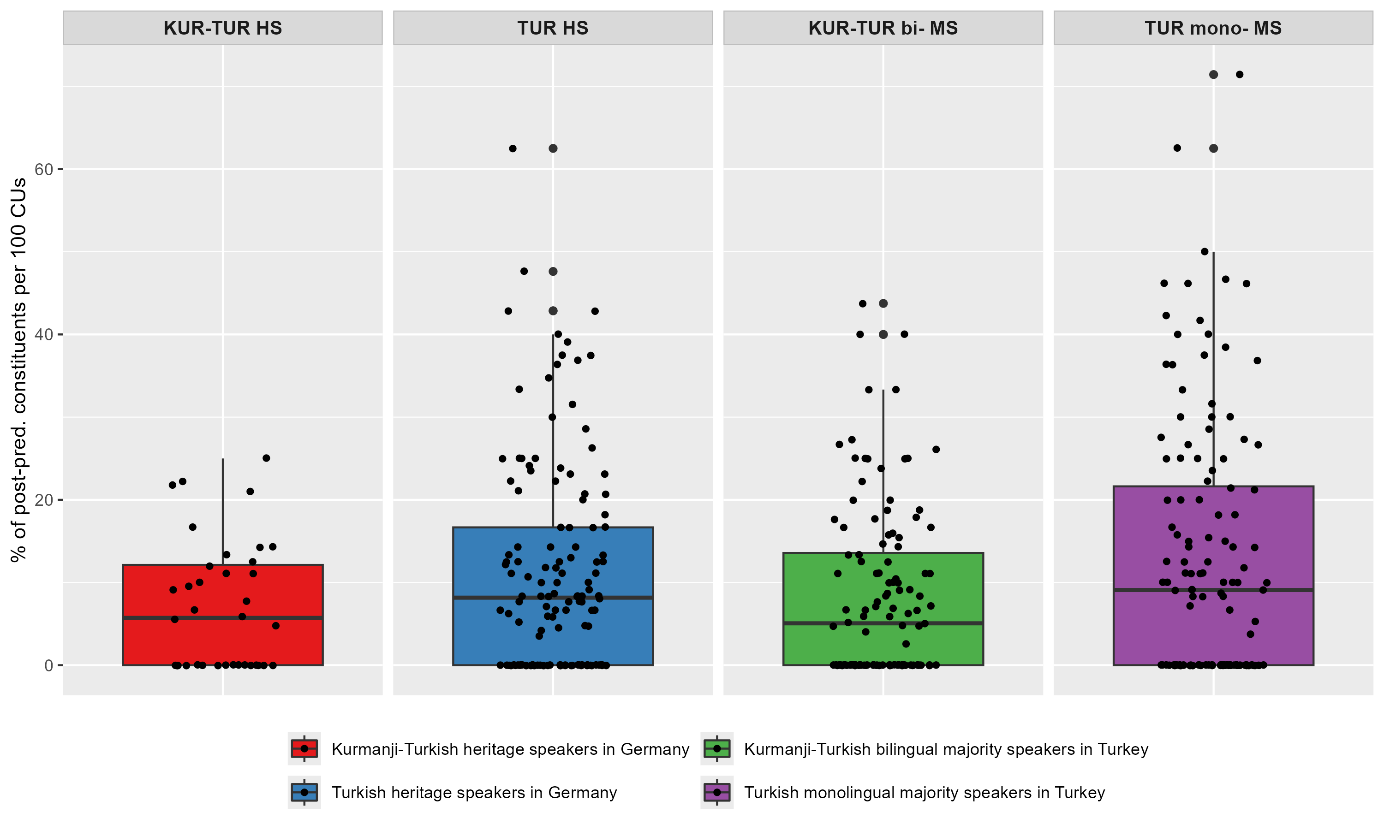
\includegraphics[width=\textwidth]{figures/iefremenko-img006.png}
\caption{\label{fig:5.1}Frequency distribution of post-predicate structures normalized per 100 communication units (CUs).}
\end{figure}

Figure~\ref{fig:5.1}\footnote{In this and subsequent figures, heritage speakers are abbreviated as HS and majority speakers as MS.} shows the frequency distribution of post-predicate structures normalized per 100 CUs across the four groups. The line inside each box shows the median, while each dot indicates the mean number of post-predicate structures per 100 CUs used by a speaker in a communicative situation, that is, there are four dots per each speaker.

Figure \ref{fig:5.1} visually illustrates that all groups use post-predicate structures, with Turkish monolinguals using them the most ($\bar{x}$ = 12.99), followed by Turkish heritage speakers (HS) in Germany ($\bar{x}$ = 11.3), Kurmanji-Turkish bilinguals in Turkey ($\bar{x}$ = 8.37), and Kurmanji-Turkish HS in Germany ($\bar{x}$ = 7.07). However, the figure also highlights high individual variation within each group: there are speakers who, in some of their productions, do not use post-predicate structures at all, and there are some speakers who employ post-predicate structures in more than 60\% of the CUs.


To further explore these observations, the analysis considers whether there is an effect of -lingualism and the societal status of Turkish on the use of the post-predicate position. A linear mixed-effects model was run to investigate this. The dependent variable in the model is the Percentage of Post-Predicate Structures. The fixed effect -Lingualism has two levels: monolinguals (Turkish monolingual speakers) and multilinguals (Turkish HS in Germany, Kurmanji-Turkish bilingual speakers in Turkey, and Kurmanji-Turkish HS in Germany). The second fixed effect, Societal Status, distinguishes between heritage and majority contexts. Participant is included as a random variable to account for individual variation among speakers.

\begin{table}
\begin{tabularx}{\textwidth}{XYY}
\lsptoprule
\textbf{Random effects:}\\
\midrule
\textbf{Groups} & \textbf{Variance} &\textbf{Standard Deviation} \\
    Participant (Intercept) & 1.03 & 1.01 \\
    Residual & 164.10 & 12.81 \\
    \midrule
% \lspbottomrule
\end{tabularx}
\begin{tabularx}{\textwidth}{l@{}rrrrr}
% \lsptoprule
\textbf{Fixed effects:}\\
\midrule
\textbf{Fixed effect} & \textbf{Estimate} & \textbf{Std. Error} & \textbf{df} & \textbf{t-value} & \textbf{\textit{p}-value} \\
(Intercept) & 15.01 & 1.94 & 100 & 7.73 & $<.0001^{***}$ \\
-Lingualism (multilingual) & -4.61 & 1.66 & 100 & -2.77 & $.006^{**}$ \\
Societal Status (majority) & -2.03 & 1.56 & 100 & -1.29 & .19 \\
\lspbottomrule
\end{tabularx}
\caption{\label{tab:key:5.1}Results of the linear mixed-effects model for percentage of post-predicate structures with multilingualism and societal status as fixed effects.}
\end{table}


Multilingualism: Multilingualism is an independent variable assigned the levels \textit{multilingual}, which includes Kurmanji-Turkish HS in Germany, Turkish HS in Germany, Kurmanji-Turkish bilinguals in Turkey, and \textit{monolingual}, which comprises Turkish monolinguals. As seen in Table \ref{tab:key:5.1}, there is a significant negative effect of multilingualism on the use of post-predicate structures (estimate: -4.61, SE=1.66, $p=.006$), meaning that multilingual speakers use fewer post-predicate structures compared to monolingual Turkish speakers.

Societal status: Societal status is an independent variable categorized into two levels: \textit{heritage}, which includes Kurmanji-Turkish heritage speakers in Germany and Turkish heritage speakers in Germany, and \textit{majority}, which consists of Kurmanji-Turkish bilinguals in Turkey and Turkish monolinguals. As shown in Table \ref{tab:key:5.1}, societal status does not significantly affect the use of post-predicate structures in Turkish.

To determine whether the negative effect of multilingualism is significant across all multilingual groups in the data, another linear mixed-effects model was conducted. In this model, the dependent variable is the Percentage of Post-Predicate Structures, while the fixed effect is Group, which consists of four levels: Kurmanji-Turkish heritage speakers in Germany (Detr), Turkish heritage speakers in Germany (Debi), Kurmanji-Turkish bilinguals in Turkey (Tubi), and Turkish monolinguals (Tumo). The Turkish monolingual group was selected as the reference level in the regression analysis because they demonstrated a significantly higher frequency of post-predicate structure usage compared to the multilingual groups. To account for individual variation in the speakers, Participant was included as the random variable. The results of this regression analysis are presented below.

\begin{table}
\begin{tabularx}{\textwidth}{XYY}
\lsptoprule
\textbf{Random effects:}\\
\midrule
\textbf{Groups} & \textbf{Variance} & \textbf{Standard} \textbf{Deviation}\\
Participant (Intercept) & 0.18 & 0.42\\
Residual & 164.10 & 12.81\\
\midrule
\end{tabularx}
\begin{tabularx}{\textwidth}{Xrrrrr}
% \lsptoprule
\textbf{Fixed effects:}\\
\midrule
\textbf{Fixed effect} & \textbf{Estimate} & \textbf{Std. Error} & \textbf{df}  & \textbf{t-value} & \textbf{\textit{p}-value}\\
Intercept & 12.98 & 1.13 & 99 & 11.44 & $<.0001^{***}$\\
Group (Debi) & -1.68 & 1.59 & 99 & -1.05 & .29\\
Group (Detr) & -5.91 & 2.42 & 99 & -2.44 & $.01^{**}$\\
Group (Tubi) & -4.61 & 1.64 & 99 & -2.80 & $.006^{**}$\\
\lspbottomrule
\end{tabularx}
\caption{\label{tab:key:5.2}Regression results for linear mixed-effects model with percentage of post-predicate structures as the dependent variable and group as the fixed effect.}
\end{table}

Group: Group is an independent variable assigned the levels \textit{Kurmanji-Turkish HS in Germany (Detr)}, \textit{Turkish HS in Germany (Debi)}, \textit{Kurmanji-Turkish bilinguals in Turkey (Tubi)}, and \textit{Turkish monolinguals (Tumo)}. The reference level is Turkish monolinguals. As seen in \tabref{tab:key:5.2}, Kurmanji-Turkish HS in Germany (Detr) and Kurmanji-Turkish bilinguals in Turkey (Tubi) tend to employ significantly fewer post-predicate structures compared to the monolinguals, but there is no significant difference between Turkish HS in Germany and Turkish monolinguals.

To summarize the findings so far, no increased frequency of the post-predicate position has been observed in multilinguals. In fact, the analysis indicates that monolinguals in Turkey are the group that employs the highest number of post-predicate structures. Furthermore, the regression analysis also revealed that while Kurmanji-Turkish HS in Germany and Kurmanji-Turkish bilinguals in Turkey tend to employ significantly fewer post-predicate structures compared to the monolinguals, there is no significant difference between Turkish HS in Germany and Turkish monolinguals. Interestingly, it is the groups with Kurmanji as the contact language that tend to use significantly fewer post-predicate structures than monolinguals. This finding may suggest the influence of Kurmanji, a predominantly SOV language, on word order in Turkish. Furthermore, the analyses indicate that societal status does not seem to influence the use of post-predicate structures, as no differences are observed between heritage and majority Turkish speakers. Finally, it is important to emphasize the considerable individual variation within these groups: some speakers do not use post-predicate structures at all in certain productions, while others employ this position in more than 60\% of their utterances.

\section[The use of post-predicate constituents in Turkish]{The use of post-predicate constituents in Turkish across communicative situations}\label{sec:key:5.2}

Thus far, observations indicate that Kurmanji-speaking groups (Kurmanji-Turkish HS in Germany and Kurmanji-Turkish bilinguals in Turkey) tend to employ post-predicate structures less frequently than non-Kurmanji-speaking groups. This suggests that Kurmanji, as an SOV language, may influence word order in Turkish, leading speakers to prefer the verb-final pattern, which is common to both languages.

However, before drawing conclusions about the influence of Kurmanji on Turkish, it is crucial to analyze the distribution of post-predicate structures across the four communicative situations, as the employment of post-predicate structures in Turkish is sensitive to formality and mode. As explained in \sectref{sec:key:3.1.1}, this position is frequently employed in informal situations, particularly in spoken mode, and there is normative pressure on its use in formal situations, especially in the written mode (\citealt{Erguvanli1984}, \citealt{Schroeder1995}). The method `Language Situations' used in this study was designed in such a way that each speaker produced narrations in four communicative situations—informal spoken, informal written, formal spoken, and formal written—that provided an opportunity to control the data for formality (formal vs. informal) and mode (spoken vs. written). The following analysis presents the frequency distribution of post-predicate structures across these four communicative situations.

\begin{figure}
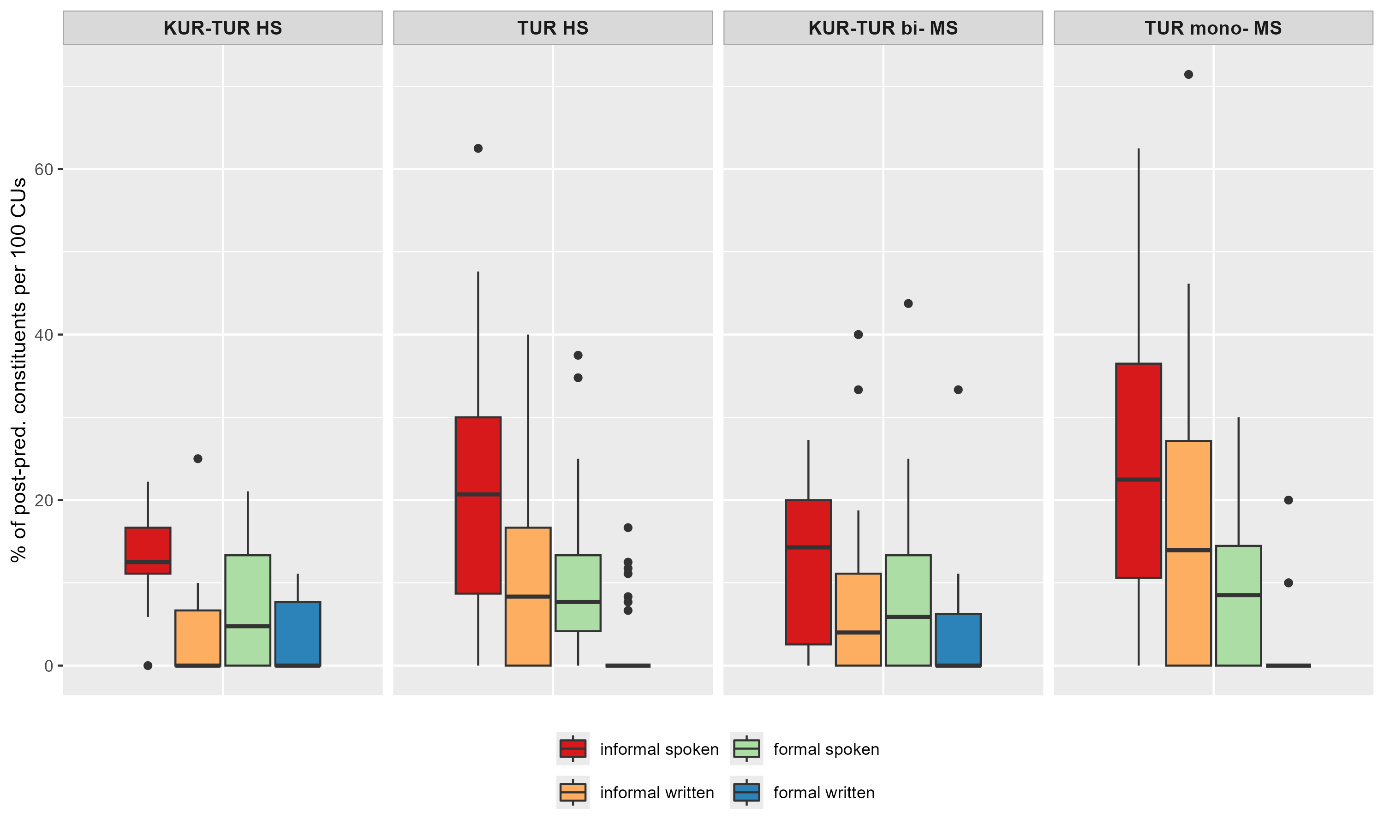
\includegraphics[width=\textwidth]{figures/iefremenko-img007.png}
\caption{Frequency distribution of post-predicate structures in Turkish, normalized to 100 CUs, with a focus on formality and mode.}
\label{fig:key:8}
\end{figure}

\figref{fig:key:8} presents the frequency distribution of post-predicate structures normalized to 100 CUs across four communicative situations. The line inside each box represents the median, while black dots, which fall outside the whiskers' range, are outliers.

\figref{fig:key:8} demonstrates a common pattern in the frequency distribution of post-predicate structures across the four groups. Across groups, the highest number of post-predicate structures occurs in the informal spoken situation: Kurmanji-Turkish HS in Germany ($\bar{x}$=12.93), Turkish HS in Germany ($\bar{x}$=21.75), Kurmanji-Turkish bilinguals in Turkey ($\bar{x}$=12.68), and Turkish monolinguals ($\bar{x}$=23.74). The informal written situation shows intermediate values: Kurmanji-Turkish HS in Germany ($\bar{x}$=5.25), Turkish HS in Germany ($\bar{x}$=10.84), Kurmanji-Turkish bilinguals in Turkey ($\bar{x}$=8.20), and Turkish monolinguals ($\bar{x}$=17.63). The formal spoken situation is also intermediate: Kurmanji-Turkish HS in Germany ($\bar{x}$=6.99), Turkish HS in Germany ($\bar{x}$=10.37), Kurmanji-Turkish bilinguals in Turkey ($\bar{x}$=9.06), and Turkish monolinguals ($\bar{x}$=9.33). The lowest number of post-predicate structures occurs in the formal written situation: Kurmanji-Turkish HS in Germany ($\bar{x}$=3.10), Turkish HS in Germany ($\bar{x}$=2.26), Kurmanji-Turkish bilinguals in Turkey ($\bar{x}$=3.54), and Turkish monolinguals ($\bar{x}$=1.25). Overall, informal written and formal spoken productions are intermediate, although in the monolingual group, the informal written mean ($\bar{x}$=17.63) is higher than the formal spoken mean ($\bar{x}$=9.33).

First of all, \figref{fig:key:8} demonstrates that there is roughly a common pattern in the frequency distribution of post-predicative structures across the four groups: the highest number of post-predicate structures is used in the informal spoken communicative situation and the lowest number of such structures is used in the formal written communicative situation. The informal written and the formal spoken productions are in the middle, with roughly a similar number of post-predicate structures. Although, in the monolingual group, the number of post-predicate structures in the informal written situation is higher than in the formal spoken one. Specifically, \textbf{\textmd{Kurmanji-Turkish HS in Germany}} produce on average $\bar{x}$={12.93} in informal spoken, $\bar{x}$={5.25} in informal written, $\bar{x}$={6.99} in formal spoken, and $\bar{x}$={3.10} in formal written. \textbf{\textmd{Turkish HS in Germany}} produce $\bar{x}$={21.75}, $\bar{x}$={10.84}, $\bar{x}$={10.37}, and $\bar{x}$={2.26}. \textbf{\textmd{Kurmanji-Turkish bilinguals in Turkey}} produce $\bar{x}$={12.68}, $\bar{x}$={8.20}, $\bar{x}$={9.06}, and $\bar{x}$={3.54}. \textbf{\textmd{Turkish monolinguals}} produce $\bar{x}$={23.74}, $\bar{x}$={17.63}, $\bar{x}$={9.33}, and $\bar{x}$={1.25} in informal spoken, informal written, formal spoken, and formal written situations, respectively.


Furthermore, \figref{fig:key:8} also shows that in terms of the frequency distribution of post-predicate structures, Turkish HS in Germany behave similarly to monolinguals, while Kurmanji-Turkish HS in Germany is similar to Kurmanji-Turkish bilinguals in Turkey, with the difference between the communicative situations being more pronounced in the first two groups. In other words, similar patterns in frequency distribution are found in the groups with Kurmanji as the contact language and in the groups without Kurmanji as the contact language.

To find out whether formality and mode modulate the employment of post-predicate structures in each of the four groups, a linear mixed-effects model was conducted. In this model, the dependent variable is the Percentage of Post-Predicate Structures, while the fixed effects include the interaction between Formality and Mode, nested within the variable Group. The variable Participant is included as a random effect to account for individual variation.\footnote{Rather than fitting a full factorial model including all possible interactions between Formality, Mode, and Group, the analysis focuses on theoretically motivated contrasts within each group. This approach allows the model to directly test whether the effects of formality and mode differ across the four speaker groups while avoiding unnecessary higher-order interactions that are not central to the hypotheses and would substantially increase model complexity.}


% ------------------------
\begin{sidewaystable}
\begin{tabularx}{\textwidth}{XYY}
\lsptoprule
\textbf{Random effects:}\\
\midrule
\textbf{Groups} & \textbf{Variance} & \textbf{Standard Deviation}\\
Participant (Intercept) & 13.06 & 3.64\\
Residual & 112.58 & 10.61\\
\midrule
\end{tabularx}
\begin{tabularx}{\textwidth}{lrrrrr}
% \lsptoprule
\textbf{Fixed effects:}\\
\midrule
% \lsptoprule
\textbf{Fixed effect} & \textbf{Estimate} & \textbf{Standard Error} & \textbf{df}  & \textbf{t-value} & \textbf{\textit{p}-value}\\
(Intercept) & 9.32 & 1.98 & 383.56 & 4.70 & < $.0001^{***}$\\
Group (Debi) & 1.04 & 2.78 & 383.56 & 0.37 & .70\\
Group (Detr) & -2.33 & 4.22 & 383.56 & -0.55 & .58\\
Group (Tubi) & -0.26 & 2.87 & 383.56 & -0.093 & .92\\
Group (Tumo)\_Formality (informal) & 14.41 & 2.65 & 297.00 & 5.43 & < $.0001^{***}$\\
Group (Debi)\_Formality (informal) & 11.38 & 2.61 & 297.00 & 4.35 & < $.0001^{***}$\\
Group (Detr)\_Formality (informal) & 5.93 & 5.00 & 297.00 & 1.18 & .23\\
Group (Tubi)\_Formality (informal) & 3.61 & 2.78 & 297.00 & 1.29 & .19\\
Group (Tumo)\_Mode (written) & -8.07 & 2.65 & 297.00 & -3.04 & $.003^{**}$\\
Group (Debi)\_Mode (written) & -8.10 & 2.61 & 297.00 & -3.10 & $.002^{**}$\\
Group (Detr)\_Mode (written) & -3.89 & 5.00 & 297.00 & -0.77 & .43\\
Group (Tubi)\_Mode (written) & -5.52 & 2.78 & 297.00 & -1.98 & $.04^{*}$\\
Group (Tumo)\_Formality (informal)\_mode (written) & 1.97 & 3.75 & 297.00 & 0.53 & 0.59\\
Group (Debi)\_Formality (informal)\_mode (written) & -2.81 & 3.69 & 297.00 & -0.76 & 0.45\\
Group (Detr)\_Formality (informal)\_mode (written) & -3.79 & 7.07 & 297.00 & -0.54 & 0.59\\
Group (Tubi)\_Formality (informal)\_mode (written) & 1.04 & 3.94 & 297.00 & 0.26 & 0.79\\
\lspbottomrule
\end{tabularx}

\caption{\label{tab:key:5.3} Regression results for linear mixed-effects model with percentage of post-predicate structures as the dependent variable and formality and mode as fixed effects.}
\end{sidewaystable}


Table \ref{tab:key:5.3} indicates that both formality and mode significantly affect the use of post-predicate structures in Turkish monolinguals and Turkish HS in Germany. Specifically, these groups tend to use more post-predicate structures in informal situations, with the highest frequencies observed in informal spoken communicative situations and lower frequencies in formal written communicative situations. In contrast, formality does not have a significant effect on post-predicate structure use in Kurmanji-Turkish HS in Germany or in Turkish bilingual speakers in Turkey, suggesting that these groups employ post-predicate structures at a more consistent rate across different communicative situations. Regarding mode, it affects the frequency of post-predicate structures in Turkish bilingual speakers in Turkey, who produce fewer post-predicate structures in the written than in the spoken communicative situations, but not in Kurmanji-Turkish HS in Germany. Overall, this suggests that while Turkish monolinguals and Turkish HS in Germany exhibit clear distinctions between communicative situations, Turkish bilingual speakers in Turkey show no significant differences in terms of formality, and Kurmanji-Turkish HS in Germany show no significant differences in either formality or mode. This pattern may be attributed to the lack of register flexibility in these groups, defined as the limited ability to adapt linguistic resources — at the lexical, syntactic, and discourse levels — according to the communicative context at hand (\citealt{QinUccelli2020}). The phenomenon of register flexibility will be further discussed in \sectref{sec:key:7.3}.

Beyond the group differences, analyzing the use of the post-predicate position across various communicative situations offers empirically grounded insights into the effect of formality and mode, discussed in the descriptive grammars of Turkish (\citealt{Erguvanli1984}, \citealt{Kornfilt1997}). As described in \sectref{sec:key:3.1.1}, the post-predicate position in an (S)OV language Turkish is typical of informal situations, while in formal situations it occurs rarely (\citealt{Erguvanli1984}, \citealt{Schroeder1995}). \citet{Erguvanli1984} notes that in more formal registers of Standard Turkish, such as legal documents and news reports -- whether in written form or broadcasted on radio and television—post-predicate structures are exceptionally uncommon. This scarcity can be attributed, in part, to normative pressures that discourage the use of post-predicate structures in formal settings.

Such claims can be partially confirmed by the data: As illustrated in \figref{fig:key:8}, a significant number of post-predicate structures are present in the formal spoken communicative situation, which is an oral witness report in the data. The example \REF{ex:key:38} below demonstrates the use of this position in the formal spoken situation by a monolingual speaker.

\ea%38
  \label{ex:key:38} Turkish, TUmo10MT\_fsT \\

        \gll Ee  karşı-dan   park-ta    yaşa-n-dı    bu  olay\\
hm  opposite-\textsc{abl}  park\textsc{-loc}  live-\textsc{pass-pst.3sg}  this  event\\
\glt ‘This incident happened hmm across the street in the park’.  \\
  \z

Interestingly, the use of post-predicate structures is frequent in the formal spoken communicative situation in the four groups, regardless of the societal status of Turkish -- whether it is the majority language or the heritage language. This indicates that even those speakers who receive education in Turkish and are exposed to its formal register employ post-predicate structures in the formal spoken situation.

On the contrary, what the data do confirm is the avoidance of the post-predicate structures in formal written texts. For instance, within the monolingual data, post-predicate structures appear in written witness reports but are exceedingly rare, with an average of just 1.25 occurrences per 100, namely four instances across 32 speakers.

The example \REF{ex:key:39} illustrates the use of the post-predicate position in the formal written situation by a monolingual Turkish speaker. In this instance, the subject of the main clause, \textit{öndeki mavi araba} (‘the blue car at the front’), appears in the post-predicate position, despite the fact that the text is a written witness report, which belongs to the formal setting.

\ea%39
  \label{ex:key:39} Turkish, TUmo32FT\_fwT \\
     \gll Köpek    yol-un    orta-sın-a    koş-unca  ani    fren\\
dog    road-\textsc{gen}  middle-\textsc{poss-dat}  run-\textsc{cvb}  sudden    brake\\
\\
\gll yap-mak  zorunda  kal-dı    \textit{ön-de-ki} \textit{mavi} \textit{araba}. \\
do\textsc{-inf}   must    stay-\textsc{pst.3sg}  front\textsc{-loc-attr}  blue  car\\
\glt ‘When the dog ran into the middle of the road, the blue car at the front had to brake immediately.’ 
  \z

The tendency to avoid post-predicate structures in the formal written situation is maintained also in the heritage groups in Germany. As illustrated in \figref{fig:key:8}, the use of post-predicate constituents in formal written situations is significantly lower than in the other situations, with an average of 2.26 instances per 100 CUs in Turkish HS in Germany and 3.1 in Kurmanji-Turkish HS in Germany. This finding is somewhat surprising, considering that heritage speakers receive little to no formal education in their heritage language and are generally not exposed to formal registers.

At the same time, the group that uses the highest number of post-predicate structures in the formal written situation is Kurmanji-Turkish bilinguals in Turkey. This finding is also surprising because, unlike heritage speakers in Germany, for bilinguals in Turkey, Turkish is the majority language, and they get formal education in it, similar to the monolinguals. However, the absolute number of such examples is too small to draw any definitive conclusions, with 10 instances across 30 speakers.

To sum up, the analysis of post-predicate structures across the four communicative situations revealed a consistent pattern across all groups: post-predicate structures are used most frequently in the informal spoken situation, followed by informal written and formal spoken situations, with their lowest occurrence in the formal written communicative situation. It is important to note that this pattern is most pronounced among Turkish monolinguals and Turkish HS in Germany. The regression model further showed that in Turkish monolinguals and Turkish HS in Germany, the use of the post-predicate position is strongly influenced by formality and mode. In contrast, Turkish bilinguals in Turkey and Kurmanji-Turkish HS in Germany show no significant difference between the formal and the informal communicative situations. Additionally, mode has no effect on post-predicate usage in Kurmanji-Turkish HS in Germany.

These findings suggest that Turkish bilinguals in Turkey and Kurmanji-Turkish HS in Germany do not distinguish between communicative situations to the same extent as Turkish monolinguals and Turkish HS in Germany. This points to the register inflexibility among speakers of Kurmanji, a phenomenon that will be discussed further in \sectref{sec:key:7.3}.

\section{Composition of post-predicate constituents}\label{sec:key:5.3}

So far, the frequency analysis showed a lower frequency of post-predicate structures in multilinguals compared to monolinguals. However, the difference is significant only in the groups that have Kurmanji in their repertoire, and these differences appear to result from blurred distinctions between formal and informal language, or between spoken and written language, in these groups.

While these findings reveal an overall trend, they do not yet clarify whether the composition of post-predicate structures differs across the groups. To address this, post-predicate structures will be analyzed with a focus on their weight, types, and semantic roles. This investigation will provide deeper insight into the linguistic developments at play and help explain why post-predicate structures are less frequent in groups with Kurmanji as a contact language compared to those without.

\subsection{Weight of post-predicate constituents in Turkish}\label{sec:key:5.3.1}

The quantitative analysis, described in \sectref{sec:key:5.1}, showed the frequency distribution of post-predicate structures in general, without considering the number of constituents that occur post-predicatively. The analysis of weight will show whether there are differences in the length of structures in the post-predicate position across the groups.

Following \citet{HaigEtAl2024}, four weight types of post-predicative constituents are distinguished: weight 1 consists of a single phonological word, weight 2 includes two phonological words, weight 3 includes three phonological words, and weight 4 comprises four or more phonological words.  Below is an example from the data for each weight type, with the post-predicate constituents in italic.\\

\begin{itemize}
\item{Weight 1:} a single phonological word.
\ea%40
  \label{ex:key:40} Turkish, TUbi14FT\_isT \\
     \gll Çocuk  araba-sı  var-dı    \textit{el-in-de}. \\
child  car-\textsc{poss}  be-\textsc{pst.3sg}  hand-\textsc{poss-loc}\\
\glt ‘A stroller was in her hands.’ 
  \z

\item{Weight 2:} two phonological words.

\ea%41
  \label{ex:key:41} Turkish, DEtr02FT\_fsT \\
     \gll Az   önce   bi   kadın-ı    gör-dü-m  \textit{eş-i-ylen}.   \textit{beraber}\\
little  before  \textsc{art}  woman-\textsc{acc}  see\textsc{-pst-1sg}  spouse-\textsc{poss-inst}  together \\
\glt ‘Just now I saw a woman together with her husband.’ 
  \z

\item{Weight 3:} three phonological words.

\ea%42
  \label{ex:key:42}  Turkish, TUmo32FT\_fsT \\
     \gll Yeni  bi  apartman  yap-ıl-dı   \\
new  \textsc{art}  block    do-\textsc{pass-pst.3sg}\\

        \gll \textit{onun}  \textit{orda-ki}    \textit{köşe-sin-de}.\\
his  there-\textsc{attr}  corner-\textsc{poss-loc}.\\
\glt ‘A new apartment building was built at that corner.’
  \z

\item{Weight 4:} four or more phonological words.

\ea%43
  \label{ex:key:43} Turkish, TUmo24MT\_isT \\
     \gll Ee  on-dan  sonra  firen-e    bas-tı    \textit{o}  \textit{gel-en} \textit{iki} \\
            hm  after  that  brake-\textsc{dat}  press\textsc{-pst.3sg}  that  come-\textsc{part}  two  \\
    \gll \textit{araba-dan}  \textit{ön-de-ki}.\\
                    car-\textsc{abl}  front\textsc{-loc-attr}  \\
\glt ‘Hm, and then braked, the front car out of those two that were coming.’ 
  \z
\end{itemize}

Elements are counted as separate words if they contribute independently to the phonological or semantic weight of a constituent, such as postpositions, discourse markers, connectors, and doubled expressions (\emph{yavaş yavaş} ‘slowly,’ \emph{sık sık} ‘often’) or the indefinite article \emph{bir} ‘a/an.’ Clitics like \textit{-y(lA)}/\textit{{}-ile} ‘with’ or \textit{-y(sA)}/\textit{{}-ise} ‘if’ are excluded because they attach phonologically to a host word and do not add independent prosodic or lexical weight.

The analysis of the weight of post-predicate constituents across the four speaker groups is presented below.

\begin{figure}
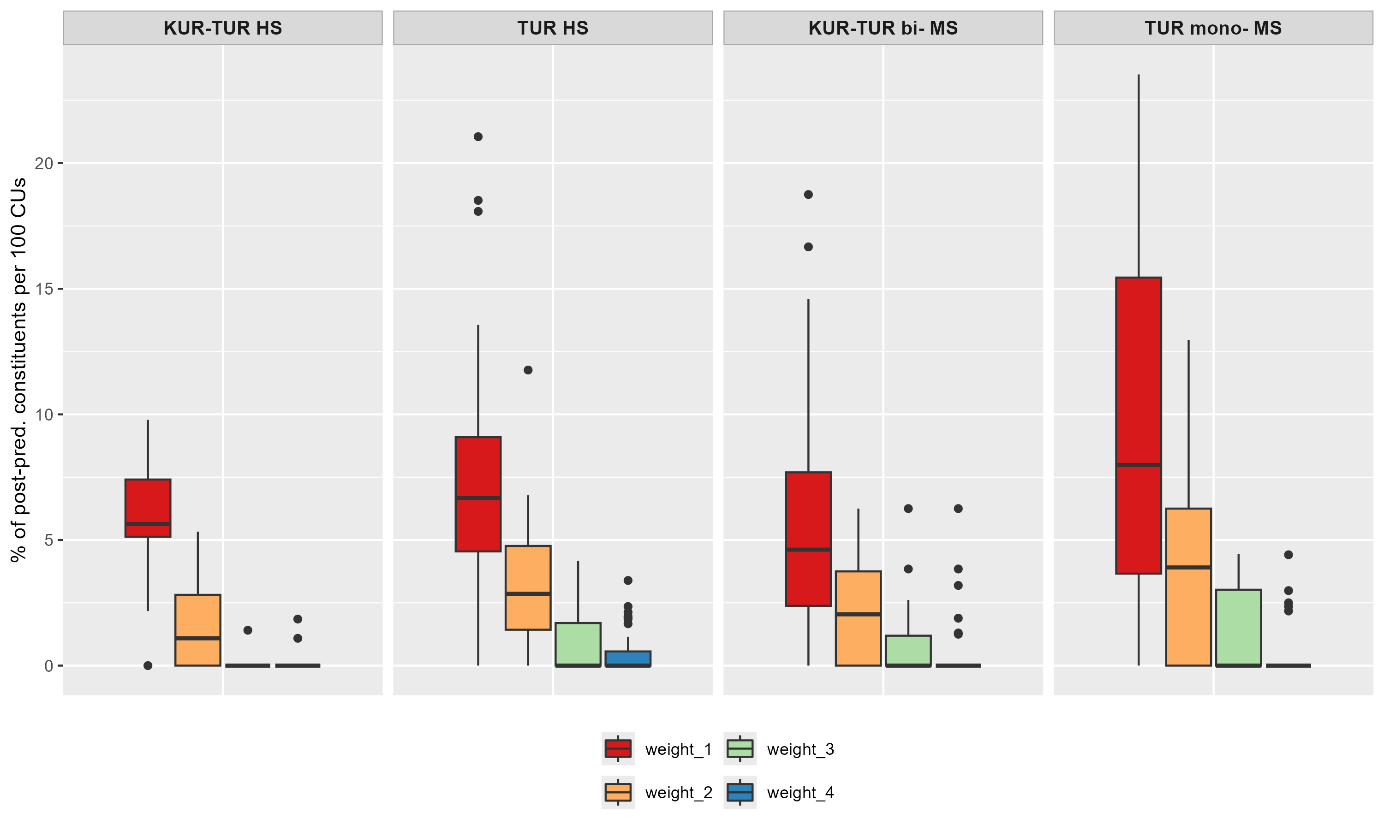
\includegraphics[width=\textwidth]{figures/iefremenko-img008.png}
\caption{Frequency distribution of post-predicate structures with a different weight.}
\label{fig:key:9}
\end{figure}

\figref{fig:key:9} shows the frequency distribution of post-predicate structures with a different weight. The line inside each box represents the median, while black dots, which fall outside the whiskers' range, are outliers. The percentage of post-predicate structures with a particular weight was calculated in relation to 100 CUs. \figref{fig:key:9} also indicates that in terms of the weight of post-predicate constituents, speakers of the four groups behave similarly. All speaker groups predominantly place one or two phonological words in the post-predicate position, and less frequently three, four, or more phonological words. Specifically, \textbf{\textmd{Kurmanji-Turkish HS in Germany}} produce on average $\bar{x}$={5.55} for weight 1, $\bar{x}${=1.75} for weight 2, $\bar{x}$={0.16} for weight 3, and $\bar{x}$={0.33} for weight 4 per 100 CUs. \textbf{\textmd{Turkish HS in Germany}} produce $\bar{x}${= 7.46, 3.06, 0.76,} and {0.51,} respectively. \textbf{\textmd{Kurmanji-Turkish bilinguals in Turkey}} produce $\bar{x}${=6.06 2.22, 0.71,} and {0.61}, while \textbf{\textmd{Turkish monolinguals}} produce $\bar{x}${=9.06, 4.00, 1.26,} {0.45} for weights 1 through 4, respectively. The whiskers also indicate significant individual variation within each group, particularly among the monolingual speakers in Turkey.

To determine whether there are differences between the groups regarding the weight of post-predicate constituents, a linear mixed-effects model was conducted, with the Percentage of Post-Predicate Structures with Different Weights as the dependent variable and Weight nested within the variable Group as the fixed effects. Treatment coding was applied to the Weight variable, while sum coding was used for the Group variable. The results of the regression analysis are presented in \tabref{tab:key:5.4}.

\begin{table}\small
\begin{tabularx}{\textwidth}{XYY}
\lsptoprule
\textbf{Random effects:}\\
\midrule
\textbf{Groups} & \textbf{Variance} & \textbf{Standard Deviation}\\
Participant (Intercept) & 1.03 & 1.01\\
Residual & 9.84 & 3.13\\
\midrule
\end{tabularx}
\begin{tabularx}{\textwidth}{Xrrrrr}
% \lsptoprule
\textbf{Fixed effects:}\\
\midrule
\textbf{Fixed effect} & \textbf{Estimate} & \textbf{Std. Error} & \textbf{df} & \textbf{t-value} & \textbf{\textit{p}-value}\\
(Intercept) & 7.03 & 0.37 & 385.59 & 18.73 & $<.0001^{***}$\\
Group (Debi) & 0.42 & 0.55 & 385.59 & 0.77 & .44\\
Group (Detr) & -1.48 & 0.86 & 385.59 & -1.72 & .08\\
Group (Tubi) & -0.97 & 0.57 & 385.59 & -1.69 & .09\\
groupDebi:Weight\_2 & -4.39 & 0.77 & 297.00 & -5.68 & $<.0001^{***}$\\
GroupDetr:Weight\_2 & -3.79 & 1.47 & 297.00 & -2.56 & $.01^{*}$\\
groupTubi:Weight\_2 & -3.84 & 0.82 & 297.00 & -4.66 & $<.0001^{***}$\\
GroupTumo:Weight\_2 & -5.06 & 0.78 & 297.00 & -6.45 & $<.0001^{***}$\\
GroupDebi:Weight\_3 & -6.70 & 0.77 & 297.00 & -8.67 & $<.0001^{***}$\\
GroupDetr:Weight\_3 & -5.39 & 1.47 & 297.00 & -3.64 & $.0003^{***}$\\
GroupTubi:Weight\_3 & -5.35 & 0.82 & 297.00 & -6.49 & $<.0001^{***}$\\
GroupTumo:Weight\_3 & -7.80 & 0.78 & 297.00 & -9.95 & $<.0001^{***}$\\
GroupDebi:Weight\_4 & -6.94 & 0.77 & 297.00 & -8.98 & $<.0001^{***}$\\
GroupDetr:Weight\_4 & -5.22 & 1.47 & 297.00 & -3.52 & $.0004^{***}$\\
GroupTubi:Weight\_4 & -5.44 & 0.82 & 297.00 & -6.61 & $<.0001^{***}$\\
GroupTumo:Weight\_4 & -8.61 & 0.78 & 297.00 & -10.98 & $<.0001^{***}$\\
\lspbottomrule
\end{tabularx}
\caption{\label{tab:key:5.4}Regression table for lmer with the dependent variable Percentage of Post-Predicate Structures with different weights and the fixed effects weight nested with Group.}
\end{table}

Group: Group is an independent variable assigned the levels \textit{Kurmanji-Turkish HS in Germany (Detr)}, \textit{Turkish HS in Germany (Debi)},\textit{Kurmanji-Turkish bilinguals in Turkey (Tubi)}, and \textit{Turkish monolinguals (Tumo)}. Sum coding was used for this variable.

Weight: Weight is an independent variable assigned the levels \textit{weight\_1}, \textit{weight\_2}, \textit{weight\_3}, and \textit{weight\_4}. The model showed that speakers of the four groups use one-word post-predicate constituents significantly more frequently than two-, three-, or four-word post-predicate constituents.

In summary, the analysis of weight revealed that post-predicate structures among the four speaker groups are generally short, typically consisting of one to two words. No differences in the weight of post-predicate constituents were observed between the groups, as the model indicated that one-word post-predicate constituents were used significantly more frequently than two-, three-, or four-word constituents across all four groups


\subsection{Types of post-predicate structures}\label{sec:key:5.3.2}

Next, the analysis turns to the types of post-predicate constituents. As outlined in \sectref{sec:key:3.1}, the post-predicate position is either canonical or the only possible placement for certain elements, including discourse markers, connectors, and particles. Consequently, it is crucial to investigate the types of post-predicate structures to assess whether the frequent use of one-word post-predicate constituents is influenced by the frequent employment of connectors and discourse markers in this position.

Furthermore, analyzing the types of post-predicate structures can provide insights into potential changes in the post-predicate domain of Turkish due to contact with other languages. As described in \sectref{sec:key:3.5}, German follows an (S)OV word order, but certain nominal constituents—such as prepositional phrases, determiner phrases, and adverbials—can be extraposed. In contrast, Kurmanji permits certain nominal constituents in the post-predicate position, including goals of motion, addressees of verbs of speech, and recipients of verbs of transfer. Therefore, if crosslinguistic influence is at play, a higher number of nominal constituents would be expected in groups where German and/or Kurmanji serves as the contact language.

Regarding the types of post-predicate structures, \citet{SchroederEtAl2024} distinguish five types of post-predicate elements in Turkish: nominal constituents (type 1), modal and manner adverbs (type 2), discourse markers, clitics, and connectors (type 3), non-finite clausal constituents (type 4), and finite clausal constituents (type 5). Additionally, post-predicate elements of each type can function as afterthoughts or self-repairs. As previously emphasized, this study focuses solely on non-clausal constituents in the post-predicate position, excluding afterthoughts and self-repairs from the analysis. Thus, the analysis of post-predicate constituents concentrates only on types 1-3. It is important to note that a single post-predicate structure may encompass two or more types (see example \ref{ex:key:44}), in such cases, each type is calculated separately.

\ea%44
  \label{ex:key:44} Turkish, TUbi03FT\_fsT \\
    \gll Ve (-)  kadın-ın  köpeğ-in-den  ötürü  ol-du   \\
and  {} woman-\textsc{gen}  dog-\textsc{poss-abl}  due\_to happen\textsc{-pst.3sg}   \\
    \gll  aslında    bu  kaza\\
    actually  this  accident  \\
\glt ‘Actually, this accident happened due to the woman’s dog.’  \\
    \z

For example, in example \ref{ex:key:44}, the adverb \textit{aslında} ‘actually’ and the noun phrase with the demonstrative \textit{bu kaza} ‘this accident’ are present, indicating that this example includes post-predicate structures of both type 1 and type 2.

\begin{figure} 
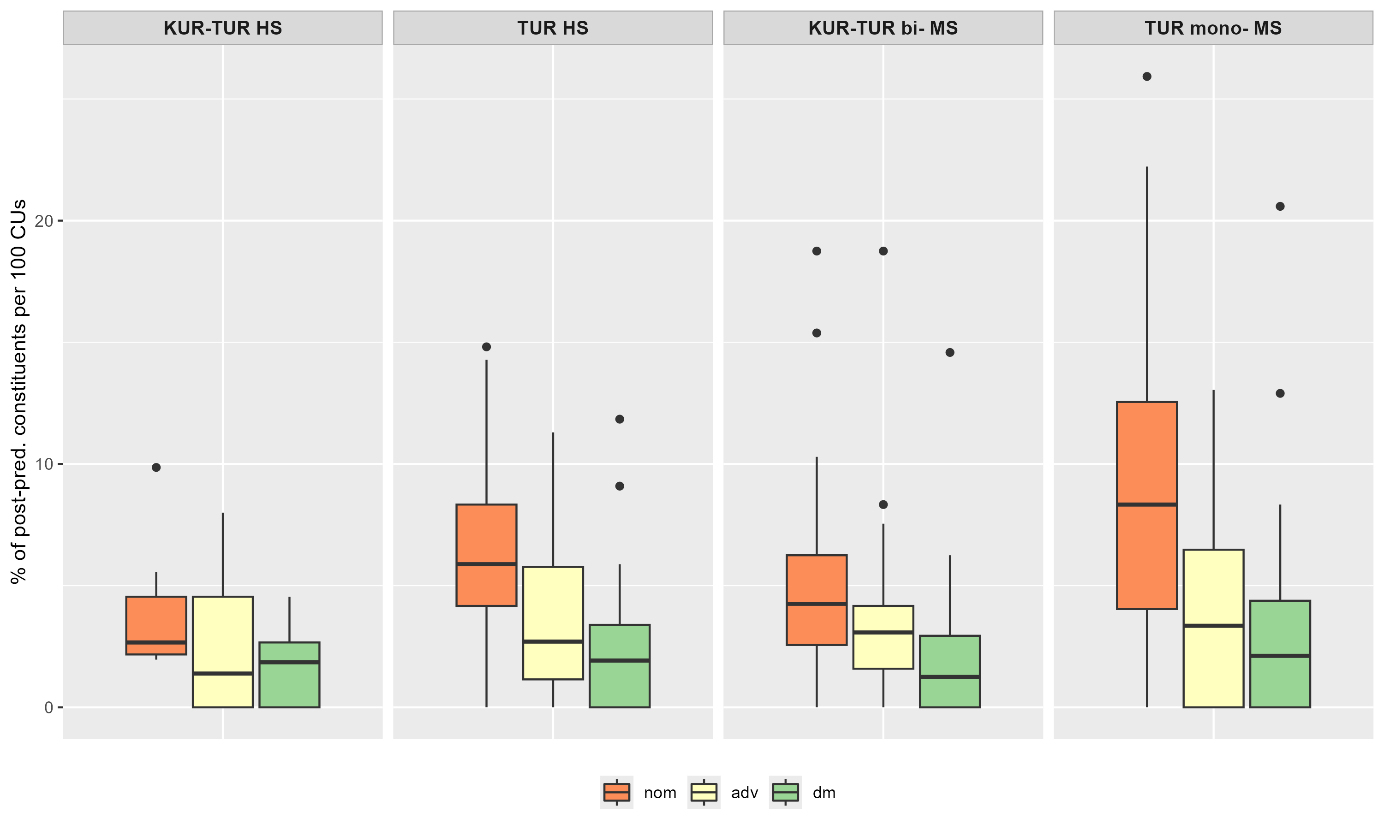
\includegraphics[width=\textwidth]{figures/iefremenko-img009.png}
\caption{\label{fig:key:10}Frequency distribution of post-predicate structures of Type 1-3 per 100 CUs. In \ref{fig:key:9}, ‘nom’ stands for nominal constituents, ‘adv’ means adverbs, while discourse markers and connectors are abbreviated as ‘dm’.}
\end{figure}
 

\figref{fig:key:10} illustrates the frequency distribution of the three types of post-predicate structures across the four groups: nominal constituents (abbreviated as \textit{nom} in the figure), modal and manner adverbs (abbreviated as \textit{adv} in the figure), and discourse markers, clitics, and connectors (abbreviated as \textit{dm} in the figure). The line within each box represents the median, while the black dots outside the whiskers indicate outliers. The percentage of post-predicate structures of each type was calculated in relation to 100 CUs.

\figref{fig:key:10} shows that the distribution of different types of post-predicate structures is relatively similar across the four groups. Nominal constituents are the most frequent type, followed by adverbs, while discourse markers and connectors occur the least frequently.

\largerpage
In terms of group differences, there are no striking disparities in the frequency distribution of adverbs, discourse markers, and connectors, although some tendencies can be observed. For nominal constituents, Turkish monolinguals exhibit the highest usage ($\bar{x}$ = 8.74), followed by Turkish heritage speakers in Germany ($\bar{x}$ = 6.78), bilingual Turkish speakers in Turkey ($\bar{x}$ = 5.10), and Kurmanji-Turkish heritage speakers in Germany ($\bar{x}$ = 3.96). For adverbs, the means are more similar across groups: Turkish monolinguals ($\bar{x}$ = 3.97), Turkish heritage speakers in Germany ($\bar{x}$ = 3.56), bilingual Turkish speakers in Turkey ($\bar{x}$ = 3.47), and Kurmanji-Turkish heritage speakers in Germany ($\bar{x}$ = 2.36). Discourse markers and connectors are the least frequent type, but still used across all groups, with the following means: Turkish monolinguals ($\bar{x}$ = 3.29), Turkish heritage speakers in Germany ($\bar{x}$ = 2.23), bilingual Turkish speakers in Turkey ($\bar{x}$ = 1.96), and Kurmanji-Turkish heritage speakers in Germany ($\bar{x}$ = 1.93). Overall, this pattern indicates that groups with Kurmanji as a contact language tend to use fewer nominal constituents in the post-predicate position compared to those without Kurmanji in their repertoire, while the distribution of adverbs and discourse markers shows less group differentiation.

To statistically verify this, a linear mixed-effects regression model was conducted with the Percentage of Post-Predicate Structures of Different Types as the dependent variable and the Type of Post-Predicate Position, nested within the variable Group, as fixed effects. Participant was included as a random variable to account for individual variation. Treatment coding was applied to the Type variable, while sum coding was used for the Group variable. The results of the regression analysis are presented in \tabref{tab:key:8}.

\begin{table}
\begin{tabularx}{\textwidth}{XYY}
\lsptoprule
\textbf{Random effects:}\\
\midrule
\textbf{Groups} & \textbf{Variance} & \textbf{Standard Deviation}\\
Participant (Intercept) & 4.20 & 2.05\\
Residual & 11.67 & 3.41\\
\midrule
% \lspbottomrule
\end{tabularx}
\begin{tabularx}{\textwidth}{Xrrrrr}
% \lsptoprule
\textbf{Fixed effects:}\\
\midrule
% \lsptoprule
\textbf{Fixed effect}  & \textbf{Estimate} & \textbf{Std. Error} & \textbf{df} & \textbf{t-value} & \textbf{\textit{p}-value}\\
(Intercept) & 3.34 & 0.45 & 260.47 & 7.36 & $<.0001^{***}$\\
Group (Debi) & 0.21 & 0.66 & 260.47 & 0.32 & .74\\
Group (Detr) & -0.98 & 1.04 & 260.47 & -0.94 & .34\\
Group (Tubi) & 0.13 & 0.69 & 260.47 & 0.15 & .85\\
GroupDebi:dm & -1.33 & 0.84 & 198.00 & -1.58 & .11\\
GroupDetr:dm & -0.42 & 1.61 & 198.00 & -0.26 & .79\\
GroupTubi:dm & -1.50 & 0.89 & 198.00 & -1.68 & .09\\
GroupTumo:dm & -0.68 & 0.85 & 198.00 & -0.80 & .42\\
GroupDebi:nom & 3.22 & 0.84 & 198.00 & 3.83 & $.0001^{***}$\\
GroupDetr:nom & 1.60 & 1.61 & 198.00 & 0.99 & .32\\
GroupTubi:nom & 1.62 & 0.89 & 198.00 & 1.81 & .07\\
GroupTumo:nom & 4.76 & 0.85 & 198.00 & 5.58 & < $.0001^{***}$\\
\lspbottomrule
\end{tabularx}
\caption{Regression table for lmer with the dependent variable Percentage of Post-Predicate Structures and the fixed effects Type nested within Group.}
\label{tab:key:8}
\end{table}

Group: Group is an independent variable assigned the levels \textit{Kurmanji-Turkish HS in Germany (Detr)}, \textit{Turkish HS in Germany (Debi)}, \textit{Kurmanji-Turkish bilinguals in Turkey (Tubi)}, and \textit{Turkish monolinguals (Tumo)}. Sum coding was used for this variable.

Type: Type is an independent variable categorized into three levels: \textit{nom} (nominal constituents), \textit{adv} (modal and manner adverbs), and \textit{dm} (discourse markers, clitics, and connectors). Treatment coding was employed, designating ‘adv’ as the reference level. The model revealed that heritage speakers of Turkish in Germany (Debi) and Turkish monolingual speakers in Turkey (Tumo) use significantly more nominal constituents. In contrast, no significant differences were observed across types for Turkish bilingual speakers in Turkey (Tubi) and Kurmanji-Turkish heritage speakers in Germany (Detr).

The regression analysis corroborated the trend illustrated in \figref{fig:key:10}, highlighting that the difference in the use of post-predicate nominal constituents is primarily between groups with and without Kurmanji as a contact language. Interestingly, the groups with no Kurmanji in their repertoire tend to use more nominal post-predicate structures compared to those with Kurmanji in their repertoire.

One of the assumptions was that a frequent use of one-word post-predicate structures among speakers in the four groups could be attributed to their frequent use of discourse markers, connectors, and particles in the post-predicate position. However, the analysis of the types of post-predicate constituents did not support this tendency across the groups. Another expectation was to find a greater number of nominal constituents in the post-predicate position among the groups with German and/or Kurmanji as a contact language compared to the monolingual group, assuming there is convergence in the post-predicate domain. Contrary to this expectation, the results revealed an opposite trend: Turkish monolinguals used the highest number of nominal constituents, while groups with Kurmanji in their repertoire employed significantly fewer nominal post-predicate structures than those without Kurmanji.

\subsection{Semantic roles of post-predicate constituents}\label{sec:key:5.3.3}
\largerpage

As described in \sectref{sec:key:3.3}, Kurmanji systematically places goals of motion, recipients of transfer, and addressees of verbs of speech in the post-predicate position. Consequently, the frequent placement of these semantic roles by Kurmanji speakers in their Turkish may indicate crosslinguistic influence in the post-predicate domain. Moreover, previous research (\citealt{Haig2020, Haignforth}) has shown that in historically SOV languages such as Turkish, goals of motion (and caused motion) are the least stable constituents. This means they are the first candidates to move into the post-predicate position in language contact situations.

In analyzing these roles, \citet{HaigEtAl2024} distinguish between various types of semantic roles. Below are examples of the most frequent ones observed in the data:

\begin{itemize}

\item Addressee of verbs of speech.

\ea%45
  \label{ex:key:45} Turkish, TUmo10MT\_isT \\
     \gll On-u  anlat-acak-tı-m  \textit{san-a} \\
it-\textsc{acc}  explain\textsc{-fut-irr-1sg}  you-\textsc{dat}\\
\glt ‘I was going to explain this to you.’
  \z

\item Benefactive -- a person who benefits or is disadvantaged by an event.

\ea%46
  \label{ex:key:46} Turkish, TUbi18MT\_isT \\
     \gll Or-da    yardım    et-ti    \textit{on-a} \\
there\textsc{-loc}  help    do-\textsc{pst.3sg}  3sg-\textsc{dat}\\
\glt‘He helped her there.’
  \z
\newpage
\item Cause -- a person/thing that is the reason for the activity.

\ea%47
  \label{ex:key:47} Turkish, TUbi06MT\_iwT \\
     \gll Az  önce  bi  köpek  ez-il-iyor-du   \textit{top} \textit{yüzünden} \\
little  before  \textsc{art}  dog  crush-\textsc{pass-prog-pst.3sg}  ball  due\_to \\
\glt ‘Just now a dog almost got run over because of a ball.’
  \z


\item Comitative -- person/thing that accompanies another person/thing in an action.


\ea%48
  \label{ex:key:48} Turkish, DEtr02FT\_fsT \\
     \gll Az   önce  bi  kadın-ı    gör-dü-m  \textit{eşi-ylen}    \textit{beraber} \\
little  before  \textsc{art}  woman-\textsc{acc}  see-\textsc{pst-1sg}  husband-\textsc{inst}    together\\
\glt ‘Just now I saw a woman together with her husband.’
  \z

\item Goals of motion and caused motion.

\ea%49
  \label{ex:key:49} Turkish, DEtr07FT\_iwT \\
     \gll Ve  {o  esnada}  köpek  top-un    arka-sın-dan    koş-tu \\
and meanwhile  dog  ball-\textsc{gen}  back-\textsc{poss-abl}  run-\textsc{pst.3sg}\\
\gll \textit{araba-nın}  \textit{peşine…}\\
 car-\textsc{gen}  after\\
\glt ‘And meanwhile, the dog ran after the ball, after the car...’
  \z

\item Static location.

\ea%50
  \label{ex:key:50} Turkish, TUmo25MT\_fsT \\
    \gll Köpek  var-dı    \textit{karşı}    \textit{taraf-ta}. \\
    dog  be-\textsc{pst.3SG}  opposite  side-\textsc{loc}  \\
    \glt ‘There was a dog on the opposite side.’
    \z

\item Source of motion.

\ea%51
  \label{ex:key:51} Turkish, DEbi18MT\_isT \\
     \gll Şöfer-ler  in-di      \textit{araba-dan} \\
driver-\textsc{pl}  {get out-\textsc{pst.3SG}} car-\textsc{abl}\\
\glt ‘The drivers got out of the car.’
  \z

\item Other -- all other categories not mentioned above. I included different semantic roles that occur very rarely in the data. It is important to mention that instances of recipients of verbs of transfer are also included in the category ‘other’ because there are only two examples of this type in the data. The reason for this lies in the methodology of the study: the video shown to the participants did not trigger the use of verbs of transfer.
\end{itemize}

\begin{figure}
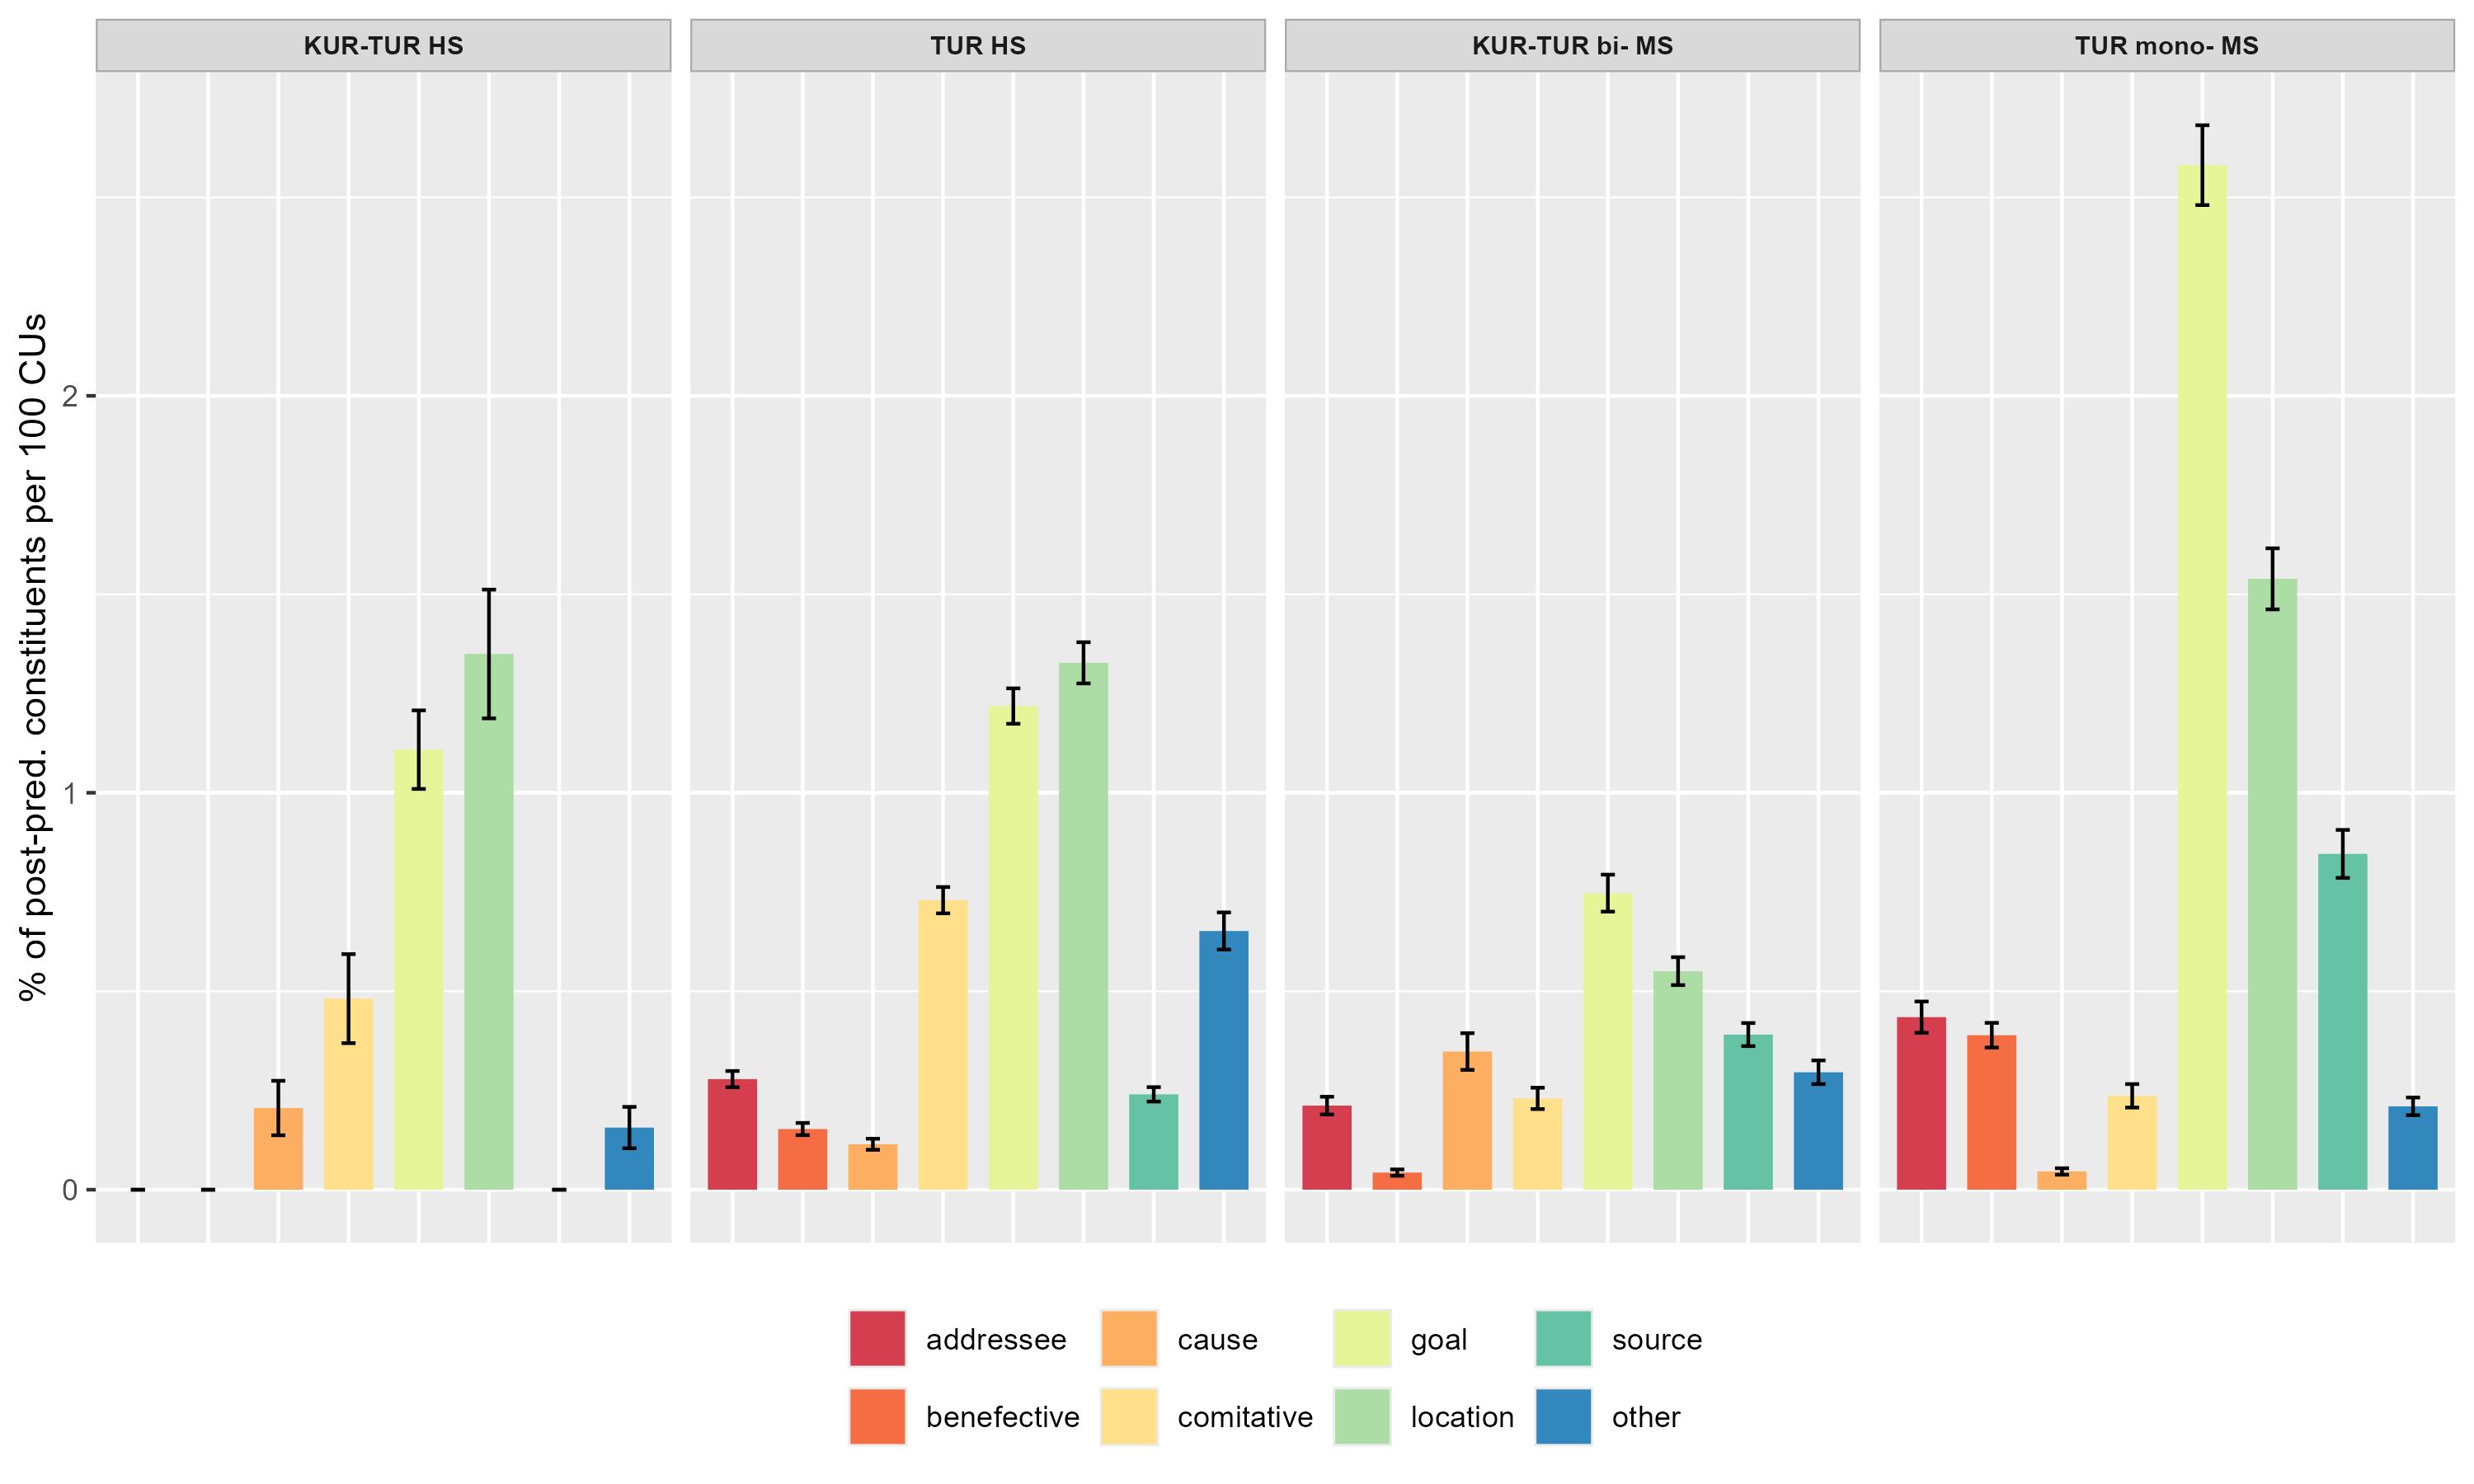
\includegraphics[width=\textwidth]{figures/iefremenko-img010.png}
\caption{\label{fig:11}Frequency distribution of nominal post-predicate structures according to their semantic role.}
\end{figure}

Figure \ref{fig:11} illustrates the mean number of nominal post-predicate structures associated with specific semantic roles, normalized by 100 CUs. Error bars indicate the standard error, providing a clearer representation of the precision of the mean estimates, particularly given the relatively low absolute numbers of nominal constituents.

According to Figure \ref{fig:11}, the most frequently occurring elements in the post-predicate position across the four groups are goals and locations. If CLI in the post-predicate domain were at play, speakers with Kurmanji in their repertoire would be expected to place motion goals, speech addressees, and recipients of transfer verbs more frequently in the post-predicate position than those without Kurmanji as a contact language. However, Figure \ref{fig:11} reveals that speakers from all groups frequently place goals of motion and caused motion in the post-predicate position, with Turkish monolingual speakers exhibiting the highest frequency of goals.

Regarding the placement of addressees of verbs of transfer in the post-predicate position, the overall numbers are quite low. Nonetheless, Figure \ref{fig:11} indicates that all groups, except for the trilinguals in Germany, do place addressees in the post-predicate position, with the monolingual group demonstrating a slightly higher percentage than the all other groups.  Given that this analysis focuses solely on nominal constituents in the post-predicate position across eight different semantic roles, there is insufficient data to run any statistical models due to the small absolute number of nominal constituents.

\subsection{Interim summary}\label{sec:key:5.3.4}

In summary, the results from the general frequency analysis of post-predicate structures, along with analyses focusing on weight, type, and semantic roles of post-predicate constituents, indicate no direct signs of CLI in the post-predicate domain. The findings reveal that monolinguals use the highest number of post-predicate structures, with heritage speakers of Turkish in Germany showing no significant differences. In contrast, speakers with Kurmanji as a contact language demonstrate a significantly lower usage of post-predicate structures, suggesting that societal status does not influence the use of these constituents, but Kurmanji as a contact language appears to have an effect.

Moreover, the analysis with the focus on the use of post-predicate structures across different communicative situations further highlights differences between groups with and without Kurmanji as a contact language. In Turkish monolinguals and heritage speakers of Turkish in Germany, the use of the post-predicate position is strongly influenced by formality and mode. In contrast, Turkish bilinguals in Turkey and Kurmanji-Turkish heritage speakers in Germany show no significant differences between formal and informal communicative situations. Furthermore, mode does not affect post-predicate usage in Kurmanji-Turkish heritage speakers in Germany. These findings suggest that Turkish bilinguals in Turkey and Kurmanji-Turkish heritage speakers in Germany do not differentiate between communicative situations to the same extent as their Turkish monolingual and Turkish heritage speakers, indicating register inflexibility among speakers of Kurmanji.

Further analysis of the composition of post-predicate positions, concentrating on weight, type, and semantic roles, indicates that post-predicate constituents across the four speaker groups are relatively light, primarily consisting of one to two words. Additionally, the analysis of the types of post-predicate constituents reveals a difference in the use of nominal constituents between groups with and without Kurmanji as a contact language. Contrary to the expectations, monolinguals employ the highest number of nominal constituents among the groups. Finally, the analysis of semantic roles shows no evidence of crosslinguistic influence in the post-predicate domain.

\section{Analysis of the information status of referents}\label{sec:key:5.4}

Finally, the analysis shifts to post-predicate structures with a focus on the information status of the referents in this position. As discussed in \sectref{sec:key:3.1}, word order in Turkish is determined by information structure, that is, the topic is usually placed in a sentence-initial position, the focus is in the immediate pre-predicate position, and background (given) information is in the post-predicate position (\citealt{Erguvanli1984}, \citealt{Issever2003}). Hence, the employment of the post-predicate position lies at the syntax-pragmatics interface.

According to the Interface Hypothesis (\citealt{SoraceSerratrice2009}, \citealt{Sorace2011}), phenomena that lie at the external interfaces—such as the syntax-pragmatics interface—are more vulnerable to change than the ones that lie at the internal interfaces in bilinguals. Previous studies showed that there are indeed dynamics at the external interfaces in heritage languages (\citealt{MontrulPolinsky2011}, \citealt{pascual_y_cabo_illogical_2012}). This section presents an analysis of the information status of elements in the post-predicate position, investigating whether information structural constraints weaken in bilingual or multilingual contexts. In addition to multilingualism, the societal status, as well as factors such as formality and mode, are explored as potential influences on the loosening of the information structural restrictions.

For the analysis of the information status of nominal constituents in the post-predicate position 20 referents that frequently appeared in the speakers' productions (e.g., dog, ball, man) were examined. For the reason that the data were elicited and all speakers were asked to retell the same video under the same conditions, defining the most frequently used referents was straightforward.\footnote{As stated in \sectref{sec:key:4.1}, the method was developed in such a way that each bi- or trilingual speaker retold the accident eight times in different communicative situations, while monolingual speakers retold the story four times. For determining the information status of nominal constituents, each narration was analyzed separately, without considering the order of elicitation. This approach might have potentially influenced the results, and this is one of the limitations of the current study.} The defined referents were annotated in the corpus using the RefLex annotation scheme developed by \citet{riester_reflex_2017}. The following types of referents were annotated: (1) “new” (first mention), (2) “given” (referent that was introduced in previous discourse context), (3) “bridging” (referent that has not explicitly been introduced but implies the referent introduced before).

\begin{figure}
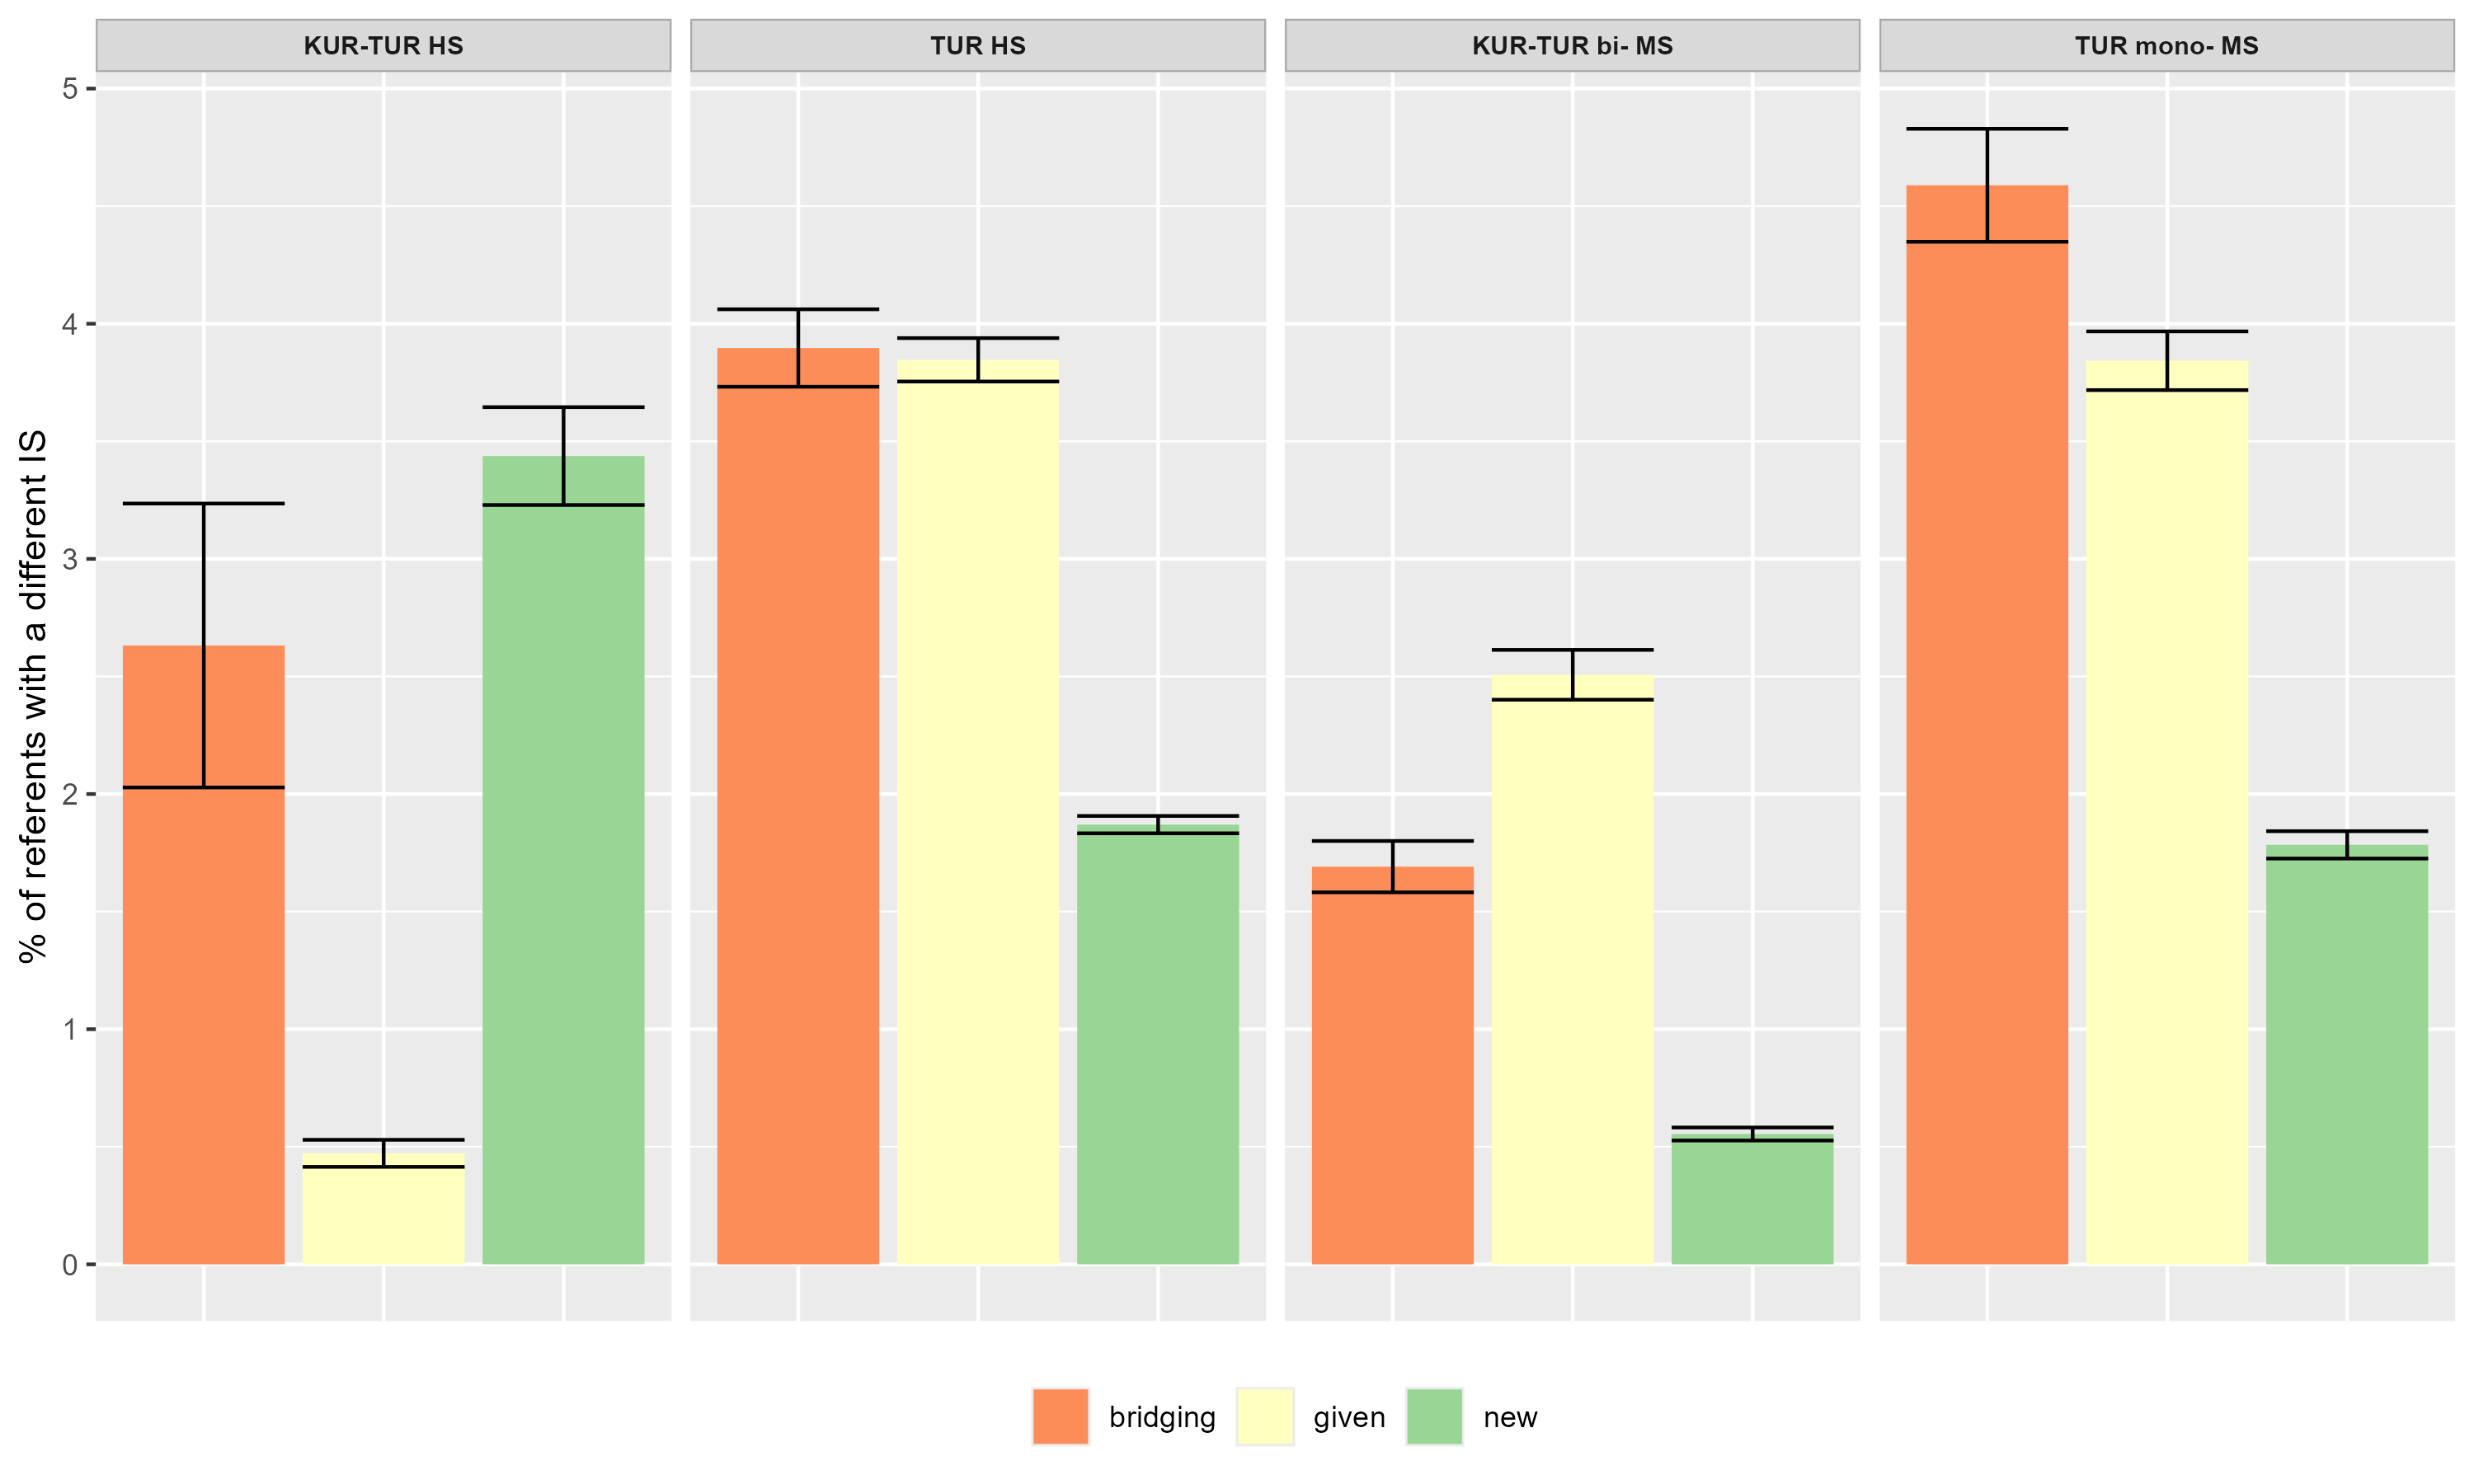
\includegraphics[width=\textwidth]{figures/iefremenko-img011.png}
\caption{\label{fig:key:12}Frequency distribution of referents in the post-predicate position according to their information status.}
\end{figure}

\figref{fig:key:12} illustrates the frequency distribution of referents in the post-predicate position based on their information status in relation to the total number of referents in the texts. Error bars indicate standard error.

The figure reveals that all types of referents appear in the post-predicate position across each group, with bridging and given referents occurring most frequently, except in the trilingual group. Previous research on word order in Turkish indicates that the post-predicate position typically accommodates given or backgrounded information, making the placement of given referents in this position unsurprising. This analysis further reveals that bridging referents—defined as those not explicitly introduced but inferable from the preceding context—also appear in the post-predicate position with a frequency similar to that of given referents. An example of bridging referents is provided in example \REF{ex:key:52}.

\newpage
\ea%52
  \label{ex:key:52} Turkish, TUmo33MT\_isT \\
    \gll iki  tane (--)  insan  yür-üyo  kadın-la  erkek. \\
two  \textsc{clf}    {}  person  walk\textsc{-prs.3sg}  woman\textsc{-inst}  man\\
\glt ‘Two persons are walking, a woman and a man.’   \\
  \z

In the example above, the referents \textit{kadın} ‘woman’ and \textit{erkek} ‘man’ are bridging because they were indirectly introduced as \textit{iki tane insan} ‘two persons’ in the same sentence.

Apart from given and bridging referents, \figref{fig:key:12} shows that speakers across all four groups also placed newly introduced referents in the post-predicate position, despite descriptive grammars of Turkish emphasizing that new information is generally not permitted in this position (\citealt{Kornfilt1997}, \citealt{GokselKerslake2004}). Example \REF{ex:key:53} further illustrates this with a case of a newly introduced referent appearing post-predicatively in the dataset.

\ea%53
  \label{ex:key:53} Turkish, DEbi06FT\_isT \\
     \gll Em (-)  onun  gir-eceğ-i    yer-de    de  böyle    bi\\
 hm  {} his  enter-\textsc{part-poss.3sg}  place-\textsc{loc}  also  like-this  \textsc{art}\\
\gll yan-ın-da     bi  ee  kadın    var-dı    köpeğ-i-yle \\
close\textsc{-poss-loc}  \textsc{art}  hm  woman    be-\textsc{pst.3sg}  dog\textsc{-poss-inst}\\
\glt ‘Hm, at the place where he was entering, so like next to it, there was a woman with her dog.’ \\
  \z

In example \REF{ex:key:53}, the referent \textit{köpeğiyle} ‘with a dog’ is a newly mentioned referent that is not retrievable from the previous context and plays an important role in the further text. As noted earlier, descriptive grammars of Turkish (\citealt{Kornfilt1997}, \citealt{GokselKerslake2004}) state that new information should not appear in the post-predicate position. However, \figref{fig:key:12} shows that speakers of the four groups, including majority Turkish speakers in Turkey, place new referents also in the post-predicate position. The group that employs new referents in the post-predicate position most frequently is Kurmanji-Turkish HS in Germany (\={x}=3.44), followed by HS of Turkish in Germany (\={x}=1.87) and Turkish monolinguals (\={x}=1.78), while the group who places new referents in the post-predicate position least frequently is Kurmanji-Turkish bilinguals in Turkey (\={x}=0.55). However, it is important to note that these occurrences remain relatively rare, with over 95\% of new referents in still appearing in the pre-predicate position. Nevertheless, since the analysis reveals that monolinguals also place new referents in the post-predicate position, bi- or multilingualism alone does not appear to be a determining factor. However, \figref{fig:key:12} suggests that societal status of Turkish may play a role, as heritage speakers place new referents in the post-predicate position more frequently than majority speakers.

To explore the effect of the societal status of Turkish and multilingualism, a linear mixed-effects model was run. The dependent variable was the Percentage of New Referents in the Post-Predicate Position, while the fixed effects included Multilingualism (multilingual vs. monolingual) and Societal Status of Turkish (heritage vs. majority). The variable Participant was included as a random variable to account for individual differences among the speakers. An overview of the regression results is presented in \tabref{tab:key:5.6}.

\begin{table}
\begin{tabularx}{\textwidth}{XYY}
\lsptoprule
\textbf{Random effects:}\\
\midrule
\textbf{Groups} & \textbf{Variance} & \textbf{Standard Deviation}\\
Participant (Intercept) & 0.70 & 0.83\\
Residual & 22.02 & 5.65\\
\midrule
\end{tabularx}
\begin{tabularx}{\textwidth}{Xrrrrr}
% \lsptoprule
\textbf{Fixed effects:}\\
\midrule
\textbf{Fixed effect} & \textbf{Estimate} & \textbf{Std. Error} & \textbf{df}  & \textbf{t-value} & \textbf{\textit{p}-value}\\
(Intercept) & 3.43 & 0.88 & 102.30 & 3.88 & $<.0001^{***}$\\
Multilingualism\\ (multilingual) & -1.23 & 0.75 & 103.04 & -1.62 & 0.10\\
Societal Status\\ (majority) & -1.65 & 0.71 & 103.40 & -2.30 & $.02^{*}$\\
\lspbottomrule
\end{tabularx}

\caption{\label{tab:key:5.6}Regression table for lmer with the dependent variable Percentage of New Referents and the independent variables Multilingualism and Societal Status.}
\end{table}

Multilingualism: Multilingualism is a binary independent variable assigned the levels \textit{multilingual} (HS of Turkish in Germany, HS of Turkish and Kurmanji in Germany, Kurmanji-Turkish bilinguals in Turkey) and \textit{monolingual} (Turkish monolinguals in Turkey) in the study. As seen in \tabref{tab:key:5.6}, there is no effect of multilingualism on the use of new referents in the post-predicate position (estimate: -1.23, SE=0.75, \textit{p} < 0.10).

Societal Status: The societal status of Turkish is a binary independent variable with the levels \textit{majority} (Kurmanji-Turkish bilinguals in Turkey and Turkish monolinguals in Turkey) and \textit{heritage} (HS of Turkish in Germany and HS of Turkish and Kurmanji in Germany). The model shows a negative effect of the majority status (estimate: -1.65, SE=0.71, \textit{p} = .02) on the employment of new referents in the post-predicate position. This means that speakers for whom Turkish is the majority language tend to place fewer new referents in the post-predicate position than heritage speakers of Turkish. In other words, heritage speakers in Germany use the post-predicate position for introducing new referents more frequently than majority speakers in Turkey.

In summary, the model confirmed that the use of new referents in the post-predicate position is not more prevalent among bi- or multilinguals compared to monolinguals. However, it revealed that groups where Turkish is the majority language, such as Kurmanji-Turkish bilinguals and Turkish monolinguals, tend to employ new referents in the post-predicate position less frequently than groups where Turkish is a heritage language. Thus, the results suggest that the loosening of information structural constraints is more likely among heritage speakers of Turkish. Interestingly, among majority speakers in Turkey, monolingual majority speakers use more new referents in the post-predicate position than their bilingual counterparts. This indicates that bilingual majority speakers tend to adhere more closely to canonical structures compared to monolinguals.

To further explore the usage of new referents in the post-predicate position across various communicative situations, the following analysis will examine the impact of formality and mode on their placement.

\begin{figure}[b]
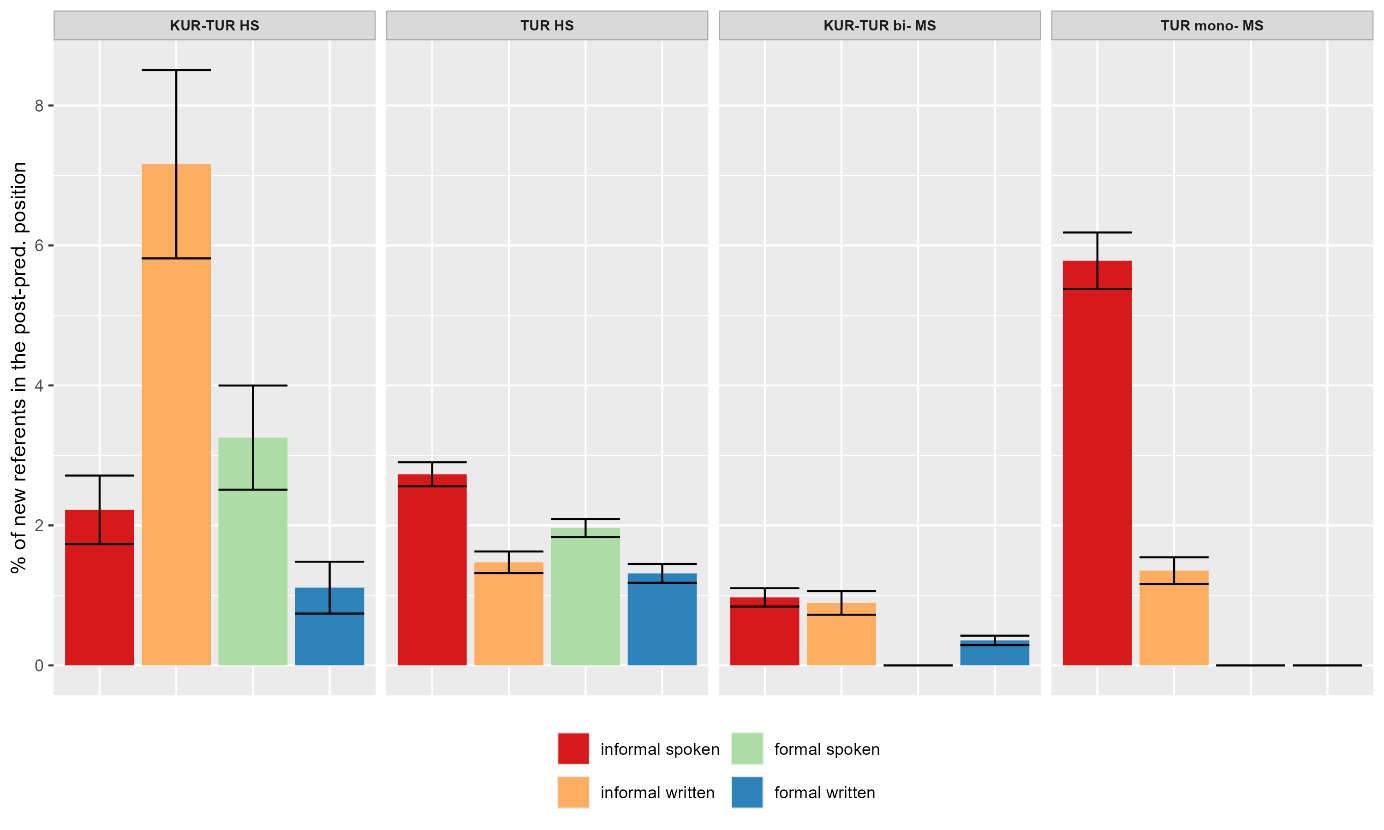
\includegraphics[width=\textwidth]{figures/iefremenko-img012.png}
\caption{\label{fig:key:13}Frequency distribution of new referents across different communicative situations.}
\end{figure}

\largerpage
\figref{fig:key:13} illustrates the frequency distribution of new referents in the post-predicate position relative to the total number of new referents in each communicative situation, with error bars representing standard error. As noted earlier, the absolute number of new referents in the post-predicate position is very low across the speaker groups. Because of this small sample size, the observed distribution should be interpreted with caution. Accordingly, no statistical model is applied, and the discussion is based solely on the patterns visible in the plot.

From \figref{fig:key:13}, it is evident that heritage speakers employ new referents across all communicative situations, while the majority speakers, particularly the monolinguals, predominantly use new referents in the informal situations. This suggests that the higher likelihood of heritage speakers using new referents in the post-predicate position is not solely attributable to the societal status of Turkish, but rather reflects a process of register inflexibility among heritage speakers, where the distinction between formal and informal or spoken and written become less pronounced.

Furthermore, the observation that majority speakers in Turkey, particularly monolinguals, tend to place new information in the post-predicate position challenges the assertions made in descriptive grammars of Turkish, which state that new referents are not permitted in the post-predicate position (\citealt{Erguvanli1984}, \citealt{GokselÖzsoy2000}, \citealt{Issever2003}). However, \citet{DogruozBackus2007} noted that, under certain conditions, focused information can indeed be positioned in the post-predicate position. They argue that focused elements may appear there when “certain linguistic devices, such as discourse markers or the particle \textit{şey}, signal that part of the focus will appear in the postverbal area, or when new information in the postverbal area is less prominent than another piece of focused information in the preverbal area” (\citealt{DogruozBackus2007}: 206).

Following \citet{DogruozBackus2007}, an examination of new referents in the post-predicate position reveals that over half (76\%, n = 35) of these new referents are secondary in relation to nominal referents introduced in the pre-predicate position. For example, in \REF{ex:key:53}, the referent \textit{köpeğiyle} ‘with a dog’ is a new mention, but it is secondary to the preceding referent \textit{bir kadın} ‘a woman.’ In contrast, the remaining 24\% (n=11) of new referents in the post-predicate position were in fact new, as demonstrated in example \REF{ex:key:54}, which features two new referents, \textit{çocuk} ‘a child’ and \textit{bir kadın} ‘a woman,’ both of which are introduced for the first time at the beginning of a narration.

\ea%54
  \label{ex:key:54} Turkish, TUbi26MT\_isT \\
\gll {az  kalsın}  bi  araba  çarp-ıyo-du  çocuk-lu  bi  kadın-a \\
almost \textsc{art}  car  hit-\textsc{prog-pst}  child\textsc{-attr} \textsc{art}  woman\textsc{-dat}\\
\glt ‘A car almost hit a woman with a child.’ \\
  \z

Thus, the analysis indicates that information structural constraints remain intact in Turkish. While new referents can appear in the post-predicate position, they primarily function as secondary elements, often linked to new referents introduced before the predicate.

In summary, the analysis of the information status of referents revealed that all groups include new referents in the post-predicate position, although the number of instances is not high. Furthermore, the majority of these new referents function as ‘less prominent’ elements related to the new referents introduced in the pre-predicate position. Besides, the analysis showed that heritage speakers of Turkish tend to place new referents in the post-predicate position more frequently than the majority speakers, but the differences lie mostly in formal situations. While majority speakers tend to avoid placing new referents in the post-predicate position in formal situations, heritage speakers place them across all communicative situations. Finally, there is also a difference between the majority speakers of Turkish in the data: the monolingual majority speakers tend to employ new referents in the post-predicate position more frequently than the bilingual majority speakers in Turkey. This observation further supports the argument that Kurmanji-Turkish bilinguals in Turkey adhere more closely to canonical language structures than monolingual speakers.

\section{Summary of the findings}\label{sec:key:5.5}

This section discusses the key findings presented in this chapter concerning word order variation in the Turkish varieties. The discussion is structured around three main aspects: (1) different language contact situations with the different intensity this contact, (2) bilingualism and the societal status of Turkish, and (3) the role of register.

The discussion begins by examining the first two factors, focusing on the role of contact languages and the impact of bilingualism and the societal status of Turkish. A quantitative analysis was conducted to calculate the number of post-predicate structures normalized per 100 CUs across the four groups. The results indicate that word order in the investigated speaker groups remains predominantly verb-final: even in the informal spoken situations, where the percentage of post-predicate structures is highest, between 75\% and 85\% of utterances are verb-final. However, it is important to note that there is significant individual variation within the groups: while there are speakers who do not use post-predicate structures in some of their productions at all, others employ this position in more than 60\% of the utterances.

Previous studies on post-predicate structures in Turkish have also found that the word order is predominantly SOV. However, these studies report varying proportions of pre- and post-predicate structures in their data. The documented frequencies of post-predicate structures range from 2\% to 45\% (e.g., \citealt{Antonova-unlu2015, Antonova-unlu2019}, \citealt{DogruozBackus2007}, \citealt{Saginsimsek2016}, \citealt{SchroederEtAl2024}, among others). The differences in the frequency distribution of post-predicate structures across these studies may be attributed to factors such as participants' age, the type of data analyzed (spontaneous vs. elicited), and the level of formality of the analyzed data. In addition, comparisons across studies are complicated by differences in analytical approaches and coding procedures.

The quantitative analysis of post-predicate structures in this study reveals that monolinguals in Turkey use the highest number of such structures. However, Turkish heritage speakers in Germany employ nearly the same frequency of post-predicate structures as the monolinguals, with no significant differences observed between the two groups. Thus, the societal status of Turkish appears to have no impact on the use of post-predicate structures. These findings align with those of \citet{DogruozBackus2007}, who also reported no significant difference in the frequency distribution of post-predicate structures between heritage Turkish in the Netherlands and monolingual Turkish speakers in Turkey.

In contrast, speakers from the two groups where Kurmanji is the contact language use significantly fewer post-predicate structures compared to the monolinguals and Turkish heritage speakers in Germany. This finding suggests that Kurmanji has an influence on Turkish, despite being a heritage language for speakers in both groups.

From the usage-based perspective, frequency is closely related to the entrenchment of a construction, which refers to the degree to which a pattern is recognized as a construction and accessed for productive use. Since Kurmanji is predominantly an SOV language that primarily places goals in the post-predicate position, the entrenchment of verb-final constructions is likely higher than that of post-predicate constructions. This difference may account for the significantly lower number of post-predicate structures in Turkish among Kurmanji speakers compared to those without Kurmanji in their linguistic repertoire.

Additionally, in German, the V2 word order pattern allows for the verb to occupy the second position in main declarative clauses with a finite main verb, which enables any constituent to be placed in the post-predicate position. However, an increase in the use of post-predicate structures among the groups in Germany has not been observed. Therefore, the tendency of the groups in this study to (not) use post-predicate structures cannot be solely attributed to the entrenchment of these constructions in the speakers' minds.

The primary difference between the contact between Turkish and German and Turkish with Kurmanji lies in the intensity of the contact. \citet{ThomasonKaufman1988} define contact intensity as the most significant social factor for predicting contact-induced language change: the more intense the contact, the greater the expected structural changes. \citet{DogruozBackus2007} also highlight the influence of social factors on the degree of borrowability, illustrating this with the example of heritage Turkish in the Netherlands. They argue that due to the relatively recent contact between Turkish and Dutch, heritage Turkish in the Netherlands experiences changes primarily at the construction level, in contrast to Gagauz, which has reached a stage of syntactic borrowing.

Similarly, the frequency analysis in this study shows that the groups with Kurmanji as the contact language employ fewer post-predicate structures than the groups where Kurmanji is not the contact language. These results indicate that the intensity of contact plays a crucial role in determining changes in the post-predicate domain. However, unlike Gagauz, Turkish in contact with Kurmanji in this study adheres to the unmarked SOV word order in Turkish. Yet, as demonstrated later on, the intensity of contact is not the only factor driving the observed changes.

In addition to the frequency differences between the groups, the analysis of the composition types of post-predicate structures—focusing on weight, types, and semantic roles—revealed no evidence of convergence in the post-predicate domain in Turkish. It was anticipated that the bilingual and trilingual groups, where Turkish is in contact with German and/or Kurmanji, would place nominal constituents in the post-predicate position more frequently than the groups in Turkey. However, the analysis indicated that Turkish monolinguals actually use the highest number of nominal constituents in the post-predicate position.

Furthermore, it was expected that the groups with Kurmanji as the contact language would exhibit a higher frequency of goals of motion, addressees, and recipients in the post-predicate position within their Turkish compared to the groups without Kurmanji in their repertoire. Contrary to this expectation, the analysis again revealed that Turkish monolinguals have the highest occurrence of goals of motion in the post-predicate position. This point will be revisited in \sectref{sec:key:7.2}.

In summary, the analysis revealed a quantitative difference in the frequency distribution of post-predicate structures between groups with and without Kurmanji in their repertoire, suggesting a potential CLI from Kurmanji to Turkish.

The third factor examined the impact of communicative situations on the use of post-predicate structures. As outlined in \sectref{sec:key:3.1.1}, the post-predicate position in Turkish is primarily employed in informal situations and spoken modes, with normative pressure discouraging its use in formal settings (\citealt{Erguvanli1984, Schroeder1995}). Overall, the frequency distribution of post-predicate structures in various communicative situations displays a similar pattern across the groups: the highest number of post-predicate structures occurs in informal spoken contexts, followed by informal written and formal spoken situations, while the lowest frequency is observed in formal written contexts.

The model revealed that while formality and mode significantly influence the use of post-predicate structures in Turkish monolinguals and Turkish HS in Germany, formality does not affect their use in Turkish bilingual speakers in Turkey or Kurmanji-Turkish HS in Germany. Similarly, while mode impacts the frequency of post-predicate structures in Turkish bilingual speakers in Turkey, it has no significant effect on Kurmanji-Turkish HS in Germany. These findings suggest that Turkish monolinguals and Turkish HS in Germany differentiate clearly between communicative situations, whereas Turkish bilingual speakers in Turkey show no notable variation based on formality, and Kurmanji-Turkish HS in Germany display no significant differences based on either formality or mode.

Heritage speakers are typically exposed to predominantly informal registers in their heritage language, often leading to register inflexibility across various linguistic phenomena (see \citealt{WieseEtAl2022}, \citealt{AlexiadouRizou2023}, \citealt{OzsoyEtAl2022}). Using the same methodology as in the current study, \citet{SchroederEtAl2024} found evidence of register inflexibility in Turkish heritage speakers in the U.S., where post-predicate structures were used at nearly the same frequency in both formal and informal settings. However, the analysis of Turkish heritage speakers in Germany in this study revealed a different pattern: while no register inflexibility was observed among Turkish HS in Germany, Kurmanji-Turkish HS showed no significant differences in the use of post-predicate structures based on either formality or mode. However, given the small sample size of the trilingual dataset (nine speakers), these findings should be interpreted with caution.

Furthermore, unlike monolingual majority speakers in Turkey, Turkish bilingual speakers in Turkey show no notable variation in the use of post-predicate structures based on formality. This difference is particularly noteworthy. Two possible explanations may account for these group differences. First, Kurmanji speakers are largely exposed to Turkish in formal situations, where verb-final word order is predominant. As a result, the preverbal construction becomes highly entrenched due to the unmarked SOV word order in both Kurmanji and formal Turkish. Second, the avoidance of post-predicate structures in informal situations by Kurmanji speakers may stem from a broader tendency among bilinguals to use canonical language forms when speaking their majority language, even in informal settings. This behavior is influenced by standard language ideology and biased attitudes toward bilinguals (\citealt{SevincDewaele2018}, \citealt{Bunk2024, bunk_anxious_2025}). These two explanations will be explored further in \sectref{sec:key:7.3}.

Beyond the frequency of post-predicate structures, this chapter examined their use with a focus on the information status of referents. As discussed in Chapter 2, Turkish word order is shaped by information structural requirements, placing background information in the post-predicate position while restricting new information after the predicate (\citealt{Erguvanli1984, Issever2003}). Consequently, the use of the post-predicate position operates at the syntax-discourse/pragmatics interface.

In bilingualism, second language acquisition, and language contact research, structural changes are often found at the interface between syntax and pragmatics/semantics \citep{Sorace2011}. In the case of Turkish, word order is strongly influenced by information structure, with topics typically sentence-initial, foci immediately pre-predicate, and background (given) information in the post-predicate position (\citealt{Erguvanli1984, Issever2003}). Because information structure governs the mapping of discourse-related features onto syntactic positions, it constitutes a phenomenon at the external syntax-pragmatics interface. Studies on heritage languages (\citealt{MontrulPolinsky2011}, \citealt{PascualEtAl2012}) suggest that external interfaces are more vulnerable than internal ones in heritage speakers. However, other studies (e.g., \citealt{Gondra2022, martynova2024ov}) challenge this claim, finding no evidence of external interface vulnerability. Therefore, this chapter addressed how information structural constraints at the external syntax-pragmatics interface affect the use of the post-predicate position in Turkish under conditions of language contact.

The analysis of Turkish word order from an information structure perspective revealed that speakers across all four groups, including monolinguals, frequently place new referents in the post-predicate position. This suggests that bilingualism and contact languages do not have an effect on the employment of new referents in the post-predicate position. This finding contradicts traditional descriptive grammars of Turkish, which assert that the post-predicate position is reserved for background information (\citealt{Erguvanli1984}, \citealt{GokselÖzsoy2000}, \citealt{Issever2003}). However, \citet{DogruozBackus2007} demonstrated that under certain conditions, Turkish allows new information in the post-predicate position—particularly when it is less prominent than other new information in the pre-predicate position. The current study supports this observation, showing that most new referents in the post-predicate position convey secondary information about a referent introduced in the pre-predicate position.

Although all groups place new referents in the post-predicate position, the analysis indicates that Turkish as a heritage language positively influences this tendency. Bilingual and trilingual heritage speakers in Germany place new referents post-predicatively more frequently than majority Turkish speakers. However, the analysis of frequency distribution across different communicative situations revealed that while majority Turkish speakers primarily use new referents in informal situations, heritage speakers employ them in both informal and formal contexts. These findings suggest a spread of informal features into formal registers rather than a vulnerability of grammatical features at the syntax-pragmatics interface in heritage speakers. The issue of register inflexibility will be revisited in \sectref{sec:key:7.3}.

Furthermore, the analysis of new referent placement shows that Kurmanji-Turkish bilinguals use fewer new referents in the post-predicate position than Turkish monolinguals. The distinction between the two groups of majority Turkish speakers in Turkey supports the conclusion that bilingualism does not drive changes at the external interface in this study. Moreover, the results further highlight the tendency of Kurmanji-Turkish bilinguals to favor more canonical structures than monolinguals. The implications of these findings for monolingual majority Turkish speakers will be explored in \sectref{sec:key:7.2}.

To summarize the findings on Turkish, the analysis revealed no quantitative differences between majority and heritage speakers in their use of the post-predicate position, either overall or across different communicative situations. Instead, heritage speakers of Turkish in Germany align with monolingual majority speakers in Turkey, while Kurmanji-Turkish heritage speakers in Germany resemble bilingual majority speakers in Turkey. The key distinction lies between speakers with and without Kurmanji in their repertoire: those with Kurmanji use fewer post-predicate structures than those without Kurmanji in their repertoire, and this difference seems to be driven by the different use of this position across communicative situations.

Although no quantitative differences in the frequency of post-predicate structures emerged between majority and heritage speakers, the analysis of referent information status revealed that heritage speakers more frequently place new referents in the post-predicate position than majority speakers. This pattern reflects the spread of informal linguistic features into formal registers among heritage speakers. As for the bilingual majority speakers in Turkey, the analysis of information status corroborated the claim that bilingual majority speakers favor more canonical structures than monolinguals, as evidenced by their lower use of new referents in the post-predicate position.


\chapter[The post-predicate position in Kurmanji in contact]{The post-predicate position in Kurmanji in contact with German and/or Turkish}\label{chap:key:6}

This chapter investigates whether there are changes in word order in Kurmanji varieties, specifically focusing on the post-predicate domain. Unlike Turkish, Kurmanji remains an underexplored heritage language, particularly in the German context. Despite being spoken by a significant number of individuals, there is a scarcity of studies examining Kurmanji, aside from those mentioned in \sectref{sec:key:2.2}. This study aims to contribute to filling this research gap.

In contrast, the Turkish context has garnered more interest in Kurmanji among researchers, particularly regarding the post-predicate domain. However, most studies have focused on speakers from villages where the majority of residents speak Kurmanji (\citealt{Dorleijn1996, Dorleijn2006}, \citealt{Haig2014}, \citealt{Haig2018, Gundogdu2019}). This study, on the other hand, centers on young adults who are Kurmanji-Turkish bilinguals living in Ankara, an urban city with a Turkish-dominant environment, and presents data from both of their languages.

Unlike Turkish, the impact of many factors on potential language change cannot be systematically investigated in Kurmanji. A major challenge lies in identifying the source of such changes—whether they are contact-induced or internally motivated. This difficulty stems largely from the scarcity of monolingual Kurmanji speakers, as the vast majority are bilingual or multilingual. Moreover, they often show stronger dominance in the majority language of their respective countries, such as Turkish, Persian, Arabic, or other contact languages (\citealt{BrizicnodateEtAl}).

Secondly, it is difficult to assess the impact of the societal status of Kurmanji. This study investigates two speaker groups: Kurmanji-Turkish bilinguals in Turkey and Kurmanji-Turkish-German trilinguals in Germany. In both cases, Kurmanji is considered a heritage language, according to the definition provided in Chapter 1. Its use is predominantly confined to informal settings, primarily within the home and among family members in both countries.

Furthermore, although Kurmanji is studied in two countries with different majority languages, Turkish serves as the contact language for both groups. However, Turkish holds different societal statuses in each country: it is a majority language in Turkey and a heritage language in Germany. Consequently, since the dominant language typically exerts a greater influence on the minority language in contact situations, a stronger impact of Turkish on Kurmanji is anticipated in Turkey compared to its influence on Kurmanji in Germany.

Moreover, the two language contexts differ from each other in terms of the intensity of contact, which is determined by the length of contact and the number of speakers in the community. Speakers of Turkic languages have likely been in contact with Kurdish speakers for over a thousand years \citep{Haig2023}. Contact between Turkish and Kurmanji predates the Ottoman Empire and intensified following the establishment of the Turkish Republic (\citealt{Yagmur2001}). Secondly, the number of individuals of Kurdish origin in Turkey is estimated at 20 million people (\citealt{Kurdish2017}). On the other hand, the contact between Kurmanji and German in Germany started in the second half of the 20\textsuperscript{th} century with the arrival of guest workers to Germany, and the number of Kurdish people in Germany is estimated at 1,300,000 (\citealt{GhaderiAlmstadt2023}). It is however unclear how many of them identify themselves as Kurds and what language(s) they speak at home.

Finally, similar to Turkish, an important factor investigated in this study is register. Unlike Turkish, the use of the post-predicate position in Kurmanji is determined by predicate semantics and is not expected to be sensitive to communicative situations. However, several reasons warrant an examination of the impact of register. First, to date, no research has explored the influence of formality and mode on word order in Kurmanji in contact with Turkish. Additionally, studies by \citet{Frommer1981} and \citet{Haig_post-predicate_EtAl2024-1} have demonstrated the effects of formality and mode on word order in Persian, a language that shares syntactic features with other Western Iranian languages, including Kurmanji. Second, the use of the post-predicate position is closely linked to formality and mode in Turkish, which serves as the contact language for both groups of Kurmanji speakers in this study. Finally, as a heritage language, Kurmanji is typically not used in formal situations, particularly when interacting with government entities, such as the police. Nonetheless, since speakers are likely aware of the effects of formality and mode on language use in the majority language, it is intriguing to explore whether they develop novel strategies in their heritage language to conform to the linguistic conventions of specific communicative situations.

In conclusion, Kurmanji is different from the heritage languages commonly studied in heritage language research. It does not have a monolingual variety and does not function as a majority language, meaning that Kurmanji speakers in both Turkey and Germany are not exposed to the various registers typically found in other languages. While this study acknowledges that many factors present in Turkish cannot be explored in the case of Kurmanji, it nonetheless establishes a foundation for future research on Kurmanji as a heritage language.

This chapter is structured as follows. First, it presents the frequency of post-predicate constituents in Kurmanji in general (\sectref{sec:key:6.1}). Next, it analyzes the use of these constituents across different communicative situations (\sectref{sec:key:6.2}). Since the post-predicate position is reserved for certain types of constituents, in \sectref{sec:key:6.3}. the chapter focuses on two main categories: goals of motion and addressees of verbs of speech. It pays particular attention to how these constituents are flagged while also considering the effect of informality and mode, and information structure on their placement. Finally, the chapter explores other (non-goal) constituents that occur in the post-predicate position. It examines their weight, type, and semantic roles, as well as their usage across various communicative contexts.

\section{Frequency distribution of post-predicate constituents in heritage Kurmanji}\label{sec:key:6.1}

The analysis begins with an overview of the frequency distribution of post-predicate constituents in Kurmanji in Turkey and Germany. It includes all instances of post-predicate position use without distinguishing between communicative situations, resulting in four data points for each speaker.

\begin{figure}
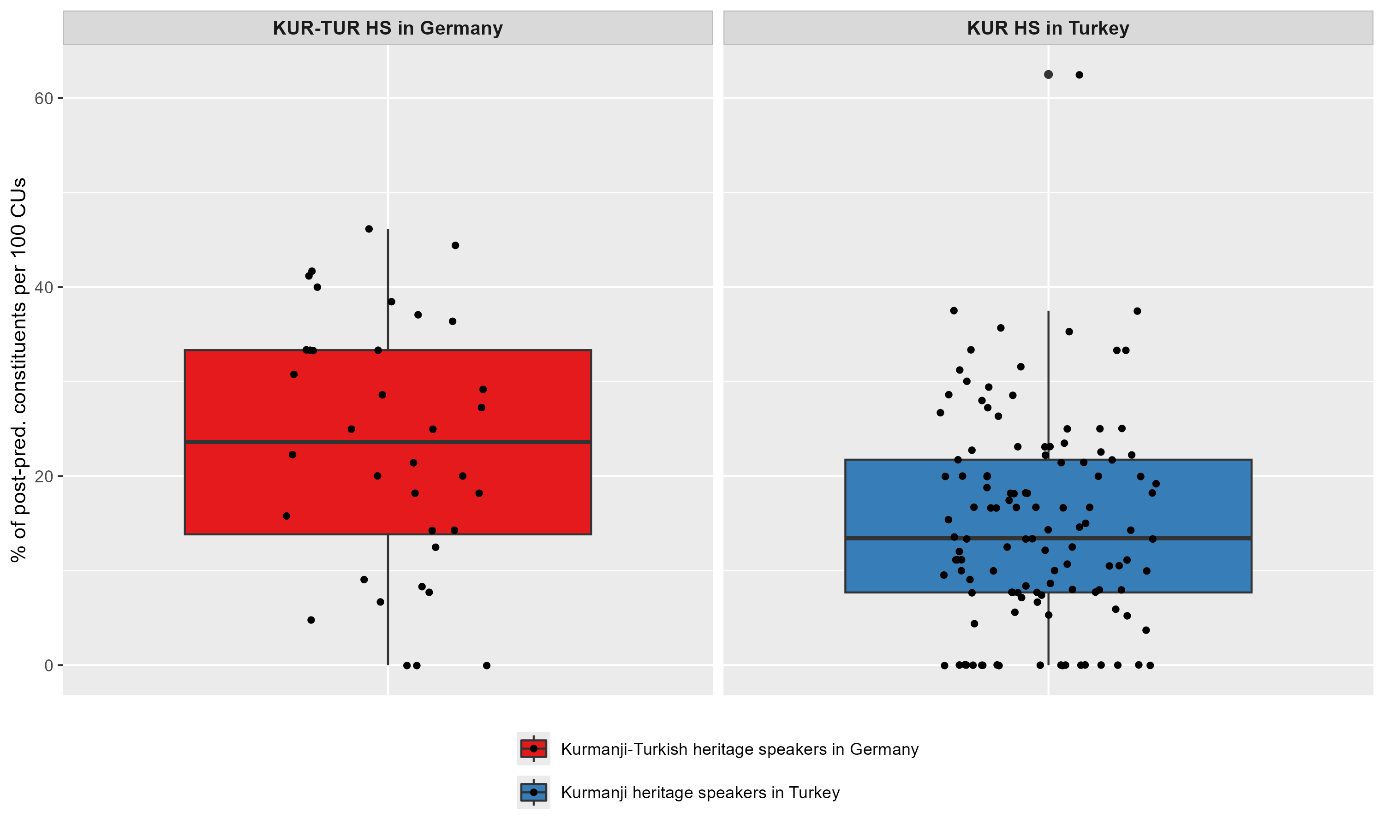
\includegraphics[width=\textwidth]{figures/iefremenko-img013.png}
\caption{\label{fig:key:14} Frequency distribution of post-predicate structures per 100 CUs.}
\end{figure}

\figref{fig:key:14} presents the frequency distribution of post-predicate structures in Kurmanji, normalized per 100 CUs, in Turkey and Germany. The line within each box shows the median, while each dot indicates the number of post-predicate structures used by a speaker in a communicative situation. Dots placed beyond the whiskers' range are outliers.

The figure reveals that the majority of utterances follow a verb-final word order. However, there is considerable individual variation among speakers: while some do not use the post-predicate position at all, others employ post-predicate structures in more than 60\% of their utterances. Additionally, the figure indicates that speakers in Germany use post-predicate structures more frequently than those in Turkey, with an average of 23.3 CUs per 100 containing a post-predicate constituent in Germany, compared to 14.9 CUs in Turkey.

To determine whether the difference in the use of post-predicate structures between the groups is significant, a linear mixed-effects model was conducted. The dependent variable is the Percentage of Post-Predicate Structures, the fixed effect is Group, while Participant is included as a random variable. The results of the regression are presented in \tabref{tab:key:10}.

\begin{table} \small
\begin{tabularx}{\textwidth}{XYY}
\lsptoprule
\textbf{Random effects:}\\
\midrule
% \lsptoprule
\textbf{Groups} & \textbf{Variance} & \textbf{Standard Deviation}\\
Participant (Intercept) & 29.5 & 5.43\\
Residual & 105.3 & 10.26\\
% \lspbottomrule
\midrule
\end{tabularx}
\begin{tabularx}{\textwidth}{Xrrrrr}
% \lsptoprule
\textbf{Fixed effects:}\\
\midrule
% \lsptoprule
\textbf{Fixed effect} & \textbf{Estimate} & \textbf{Std. Error} & \textbf{df}  & \textbf{t-value} & \textbf{\textit{p}-value}\\
Intercept & 23.27 & 2.49 & 37.00 & 9.34 & $<.0001^{***}$\\
Group (Tubi) & -8.39 & 2.83 & 37.00 & -2.95 & $.005^{**}$\\
\lspbottomrule
\end{tabularx}
\caption{Regression table for lmer with the dependent variable Percentage of Post-Predicate Structures and the independent variable Group.}
\label{tab:key:10}
\end{table}

Group: Group is an independent variable assigned the levels \textit{Kurmanji-Turkish HS in Germany (Detr)} and \textit{Kurmanji HS in Turkey (Tubi)}. As seen in \tabref{tab:key:10}, the result of the regression analysis shows that Kurmanji speakers in Turkey tend to employ significantly fewer post-predicate structures compared to Kurmanji speakers in Germany.

The analysis reveals that Kurmanji speakers in Germany use significantly more post-predicate constituents than those in Turkey. However, since the post-predicate position in Kurmanji is primarily reserved for certain indirect objects, it is not considered non-canonical. Moreover, the reasons behind the higher frequency of post-predicate constituents among speakers in Germany remain unclear. One possibility is that the distribution of these structures differs across communicative situations in each group, similar to patterns observed in Turkish. Another potential explanation could be differences in the types of post-predicate structures used by each group. To explore this further, the following sections present the analysis of the distribution of post-predicate structures across communicative situations and then focus on the different types of post-predicate constituents.

\section[The use of post-predicate constituents in Kurmanji]{The use of post-predicate constituents in Kurmanji across different communicative situations}\label{sec:key:6.2}

So far, the analysis indicates that heritage speakers of Kurmanji in Germany use more post-predicate structures than speakers in Turkey. To investigate whether communicative situations, i.e. formality and mode, affect the frequency differences between the groups, the frequency distribution of post-predicate structures was analyzed across four communicative contexts: informal spoken, informal written, formal spoken, and formal written. The results are presented in \figref{fig:key:15}.

\begin{figure}
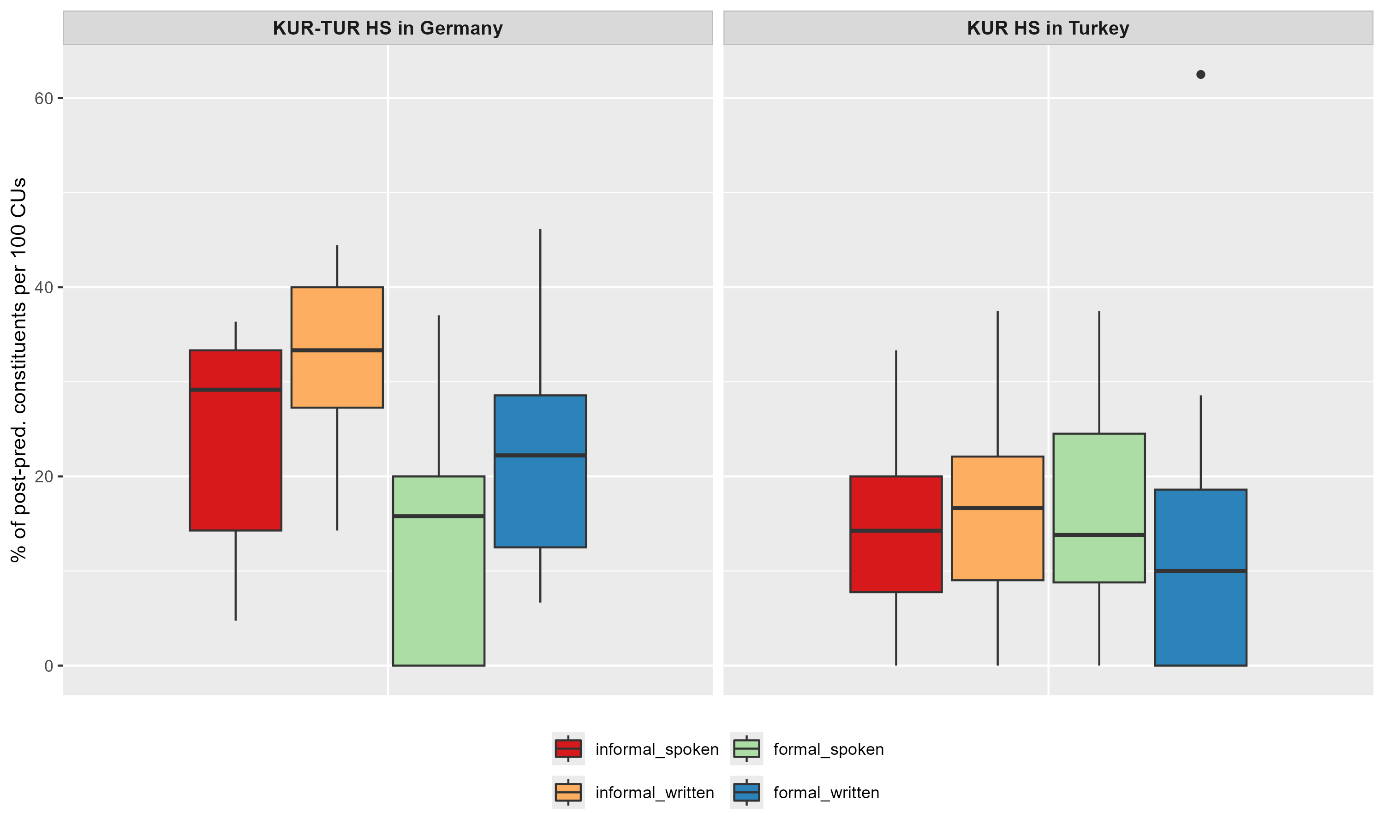
\includegraphics[width=\textwidth]{figures/iefremenko-img014.png}
\caption{\label{fig:key:15}Frequency distribution of post-predicate structures in Kurmanji in two country groups across different communicative situations.}
\end{figure}

\figref{fig:key:15} illustrates the frequency distribution of post-predicate structures across communicative situations in Turkey and Germany, normalized per 100 CUs. The line within each box shows the median, while the whiskers extended from the box indicate the minimum and maximum values. Dots falling outside the whisker range are outliers.

The visual patterns in the frequency distribution differ between the groups, and the descriptive means confirm these tendencies. For Kurmanji heritage speakers in Turkey, the use of post-predicate structures remains relatively consistent across communicative situations, with {means} ranging from $\bar{x}$ =12.62\% in the formal written situation to $\bar{x}$ =16.66\% in the formal spoken situations, and little difference between the informal spoken ($\bar{x}$={14.32\%}) and informal written ($\bar{x}$ = {15.91\%}) situations. In contrast, Kurmanji-Turkish heritage speakers in Germany show clearer situational differences. They employ post-predicate structures most frequently in the informal written context ($\bar{x}${=33.09}{\%}), followed by the informal spoken ($\bar{x}$ = {23.25\%}) and the formal written ($\bar{x}$ = {23.40\%}) situations, while the lowest mean is found in the formal spoken situations ($\bar{x}$ = {13.35\%}). Notably, speakers in Germany rely on the post-predicate position far more often in the informal written mode than in any other setting.

To determine the effects of formality and mode on the use of post-predicate structures among the two groups of Kurmanji speakers, a linear mixed-effects model was conducted. The dependent variable was the Percentage of Post-Predicate Structures, with fixed effects for the interaction between Formality (formal vs. informal) and Mode (spoken vs. written) nested within the variable Group. The variable Participant was included as a random effect. The results of the regression analysis are presented in \tabref{tab:key:11}.

\begin{table}[t]
\begin{tabularx}{\textwidth}{XYY}
\lsptoprule
\textbf{Random effects:}\\
\midrule
\textbf{Groups} & \textbf{Variance} & \textbf{Standard Deviation}\\
Participant (Intercept) & 32.68 & 5.71\\
Residual & 92.55 & 9.62\\
% \lspbottomrule
\midrule
\end{tabularx}
% \vspace{0.5em}
\begin{tabularx}{\textwidth}{lrrrrr}
% \lsptoprule
\textbf{Fixed effects:}\\
\midrule
% \lsptoprule
\textbf{Fixed effect} & \textbf{Estimate} & \textbf{Std. Error} & \textbf{df}  & \textbf{t-value} & \textbf{\textit{p}-value}\\
Intercept & 13.47 & 3.73 & 122.89 & 3.56 & $<.0001^{***}$\\
\addlinespace[0.5em]
Group (Tubi) & 3.31 & 4.25 & 122.89 & 0.78 & .43\\
\addlinespace[0.5em]
Group (Detr)\_\\Formality (informal) & 9.90 & 4.53 & 111.00 & 2.18 & $.03^{*}$\\
\addlinespace[0.5em]
Group (Tubi)\_\\Formality (informal) & -2.33 & 2.48 & 111.00 & -0.94 & .34\\
\addlinespace[0.5em]
Group (Detr)\_\\Mode (written) & 10.05 & 4.53 & 111.00 & 2.22 & $.03^{**}$\\
\addlinespace[0.5em]
Group (Tubi)\_\\Mode (written) & -4.04 & 2.48 & 111.00 & -1.63 & .10\\
\addlinespace[0.5em]
Group (Detr)\_\\Formality (informal)\_\\Mode (written) & -0.22 & 6.41 & 111.00 & -0.03 & .97\\
\addlinespace[0.5em]
Group (Tubi)\_\\Formality (informal)\_\\Mode (written) & 5.63 & 3.51 & 111.00 & 1.60 & .11\\
\lspbottomrule
\end{tabularx}
\caption{\label{tab:key:11}Regression table for lmer with the dependent variable Percentage of Post-Predicate Structures and the independent variables Formality and Mode.}
\end{table}

Formality: Formality is a binary independent variable categorized as \textit{formal} and \textit{informal} in this study. As shown in \tabref{tab:key:11}, formality significantly influences the use of post-predicate structures in Kurmanji speakers in Germany, with the speakers tending to employ post-predicate constituents more frequently in the informal communicative situations.

Mode: Mode is also a binary independent variable, consisting of \textit{spoken} and \textit{written} categories. Similar to formality, mode affects the use of the post-predicate position, but this influence is observed only among Kurmanji speakers in Germany, where the speakers are more likely to use the post-predicate position in the written communicative situations.

Thus, the regression analysis confirms the observations from the plot: while in Kurmanji speakers in Turkey mode and formality do not have an effect on the employment of the post-predicate position, Kurmanji speakers in Germany are more likely to use the post-predicate position in the informal and written communicative situations. The findings from the Kurmanji group in Turkey are not surprising, as the use of the post-predicate position in Kurmanji is determined by predicate semantics and is therefore not expected to be subject to register variation. In contrast, the observations in Kurmanji speakers in Germany are interesting and challenging to explain. While the increased use of post-predicate constituents in the informal communicative situations aligns with the patterns found in Turkish and reported in studies on German, the higher frequency of these structures in the written situations compared to the spoken ones remains unclear. However, it is important to note that the number of speakers in this group is smaller than in the other groups, suggesting that the observed frequencies could change with more data.

\section{Types of post-predicate constituents in Kurmanji}\label{sec:key:6.3}

The analysis now moves to the types of post-predicate constituents in Kurmanji. As stated in \sectref{sec:key:3.3}, the use of the post-predicate position in Kurmanji is reserved for certain indirect objects, namely, locational goals of verbs of motion and verbs of caused motion, goals of verbs of transfer and addressees of verbs of speech (\citealt{Haig2014, HaigThiele2014, Haig2018, Gundogdu2019}). The following section examines the extent to which argument type influences the use of the post-predicate position in Kurmanji. Additionally, the analysis explores whether the more frequent use of post-predicate structures among speakers in Germany, compared to those in Turkey, is driven by differing preferences for argument types in the post-predicate position.

\begin{figure}
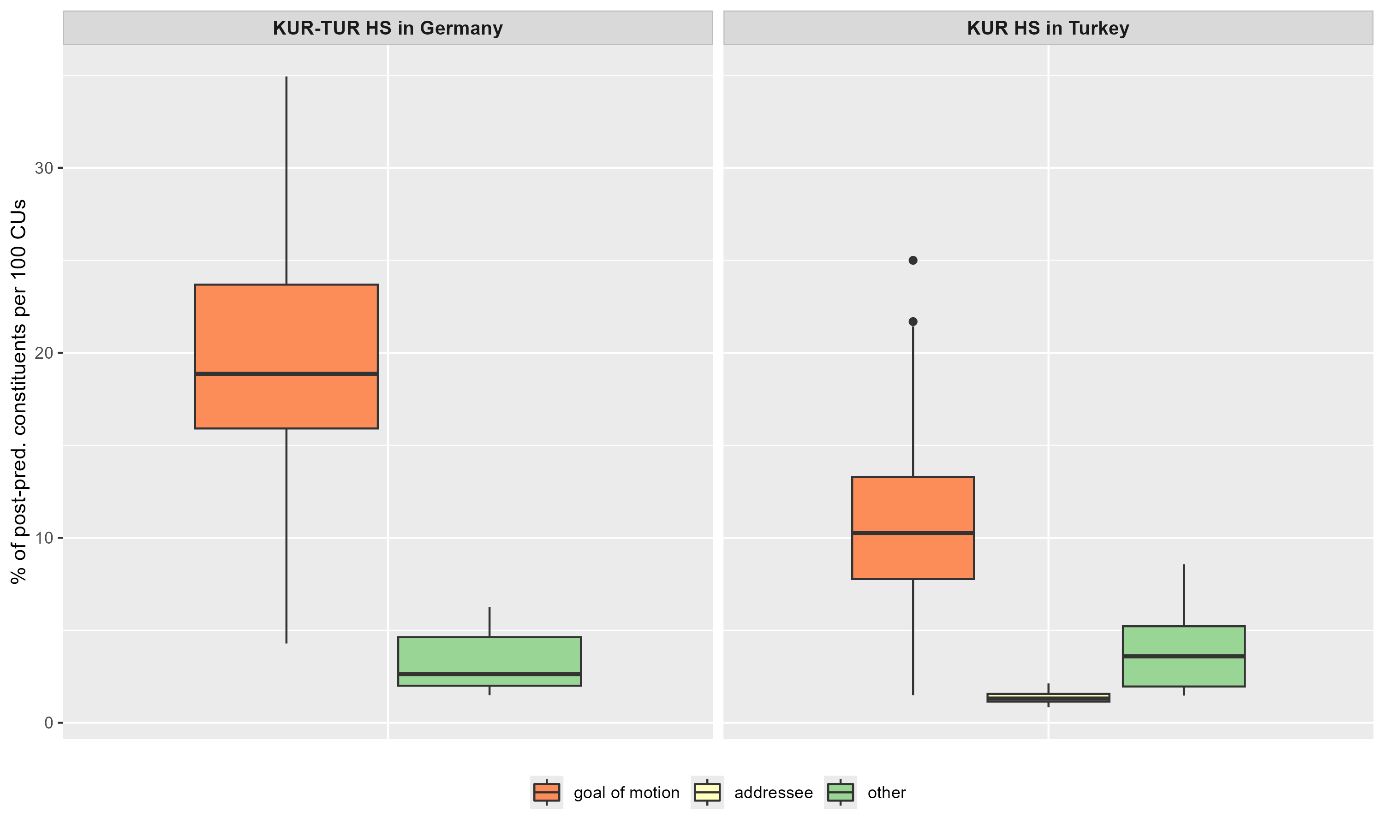
\includegraphics[width=\textwidth]{figures/iefremenko-img015.png}
\caption{\label{fig:key:16}Types of post-predicate structures in Kurmanji in two country groups.}
\end{figure}

\figref{fig:key:16} presents the frequency distribution of different types of arguments in the post-predicate position in Kurmanji as spoken in Turkey and Germany, normalized per 100 CUs. The line inside each box represents the median, while the whiskers extend to the minimum and maximum values. Dots falling outside the whisker range indicate outliers.

The figure visualizes two of the three possible types of arguments: goals of motion (shown in orange) and addressees of verbs of speech (shown in yellow). The third type—recipients of verbs of transfer—occurs very rarely in the dataset, as the video shown to participants did not elicit the use of transfer verbs. Consequently, as seen in \figref{fig:key:16}, no instances of recipients of verbs of transfer appear in the post-predicate position.

Beyond these argument types, the analysis shows that other constituents can also appear post-predicatively in Kurmanji (shown in green). These will be discussed later in this chapter (\sectref{sec:key:6.3.6}).

The descriptive means confirm that in both country groups, goals of motion are the most frequent type in the post-predicate position. For Kurmanji heritage speakers in Turkey, goals of motion appear with $\bar{x}${=11.33}{\%}, followed by other constituents ($\bar{x}$={4.01\%}) and addressees of speech ($\bar{x}$={1.40\%}). In contrast, Kurmanji-Turkish heritage speakers in Germany use goals of motion more frequently overall ($\bar{x}$={19.61\%}), while other constituents occur with $\bar{x}$={3.30\%}, no addressees of verbs of speech are attested in this group. However, these differences in frequency distribution across argument types do not necessarily reflect the general distribution of post-predicate constituents in Kurmanji. Rather, they may partly result from the data collection method: the video shown to participants featured significant movement, minimal interaction, and virtually no transfer between the actors. As a result, the data predominantly show goals of motion, followed by addressees of speech, with almost no occurrences of recipients.


\subsection{Goals of motion and caused motion}\label{sec:key:6.3.1}

The following section takes a closer look at the goals of motion and caused motion found in the data. As outlined in \sectref{sec:key:3.3}, goals of motion in Kurmanji can be flagged either with the oblique case or an adposition. Notably, these two types differ in their placement relative to the verb. Case-flagged goals must appear immediately after the predicate and cannot precede it (\citealt{Haig2014, Gundogdu2019}). In contrast, the position of adpositional goals is more flexible and depends on the type of adposition and the dialect \citep{Haig2014}. \citet{Asadpour2021} further highlights that beyond flagging and regional variation, additional factors influence the positioning of goal arguments, with information structure playing a particularly significant role. However, these findings are based on Mukri Kurdish, spoken in Iran. Hence, this section will explore the effects of factors such as flagging, formality and mode and information structure on the employment of goals of (caused) motion in the post-predicate position.

First, the analysis focuses on flagging, presenting the frequency distribution of the most common argument type in the data: goals of verbs of motion and caused motion. These goals are marked either by case or an adpositional phrase and can appear before or after the predicate.

\begin{figure}
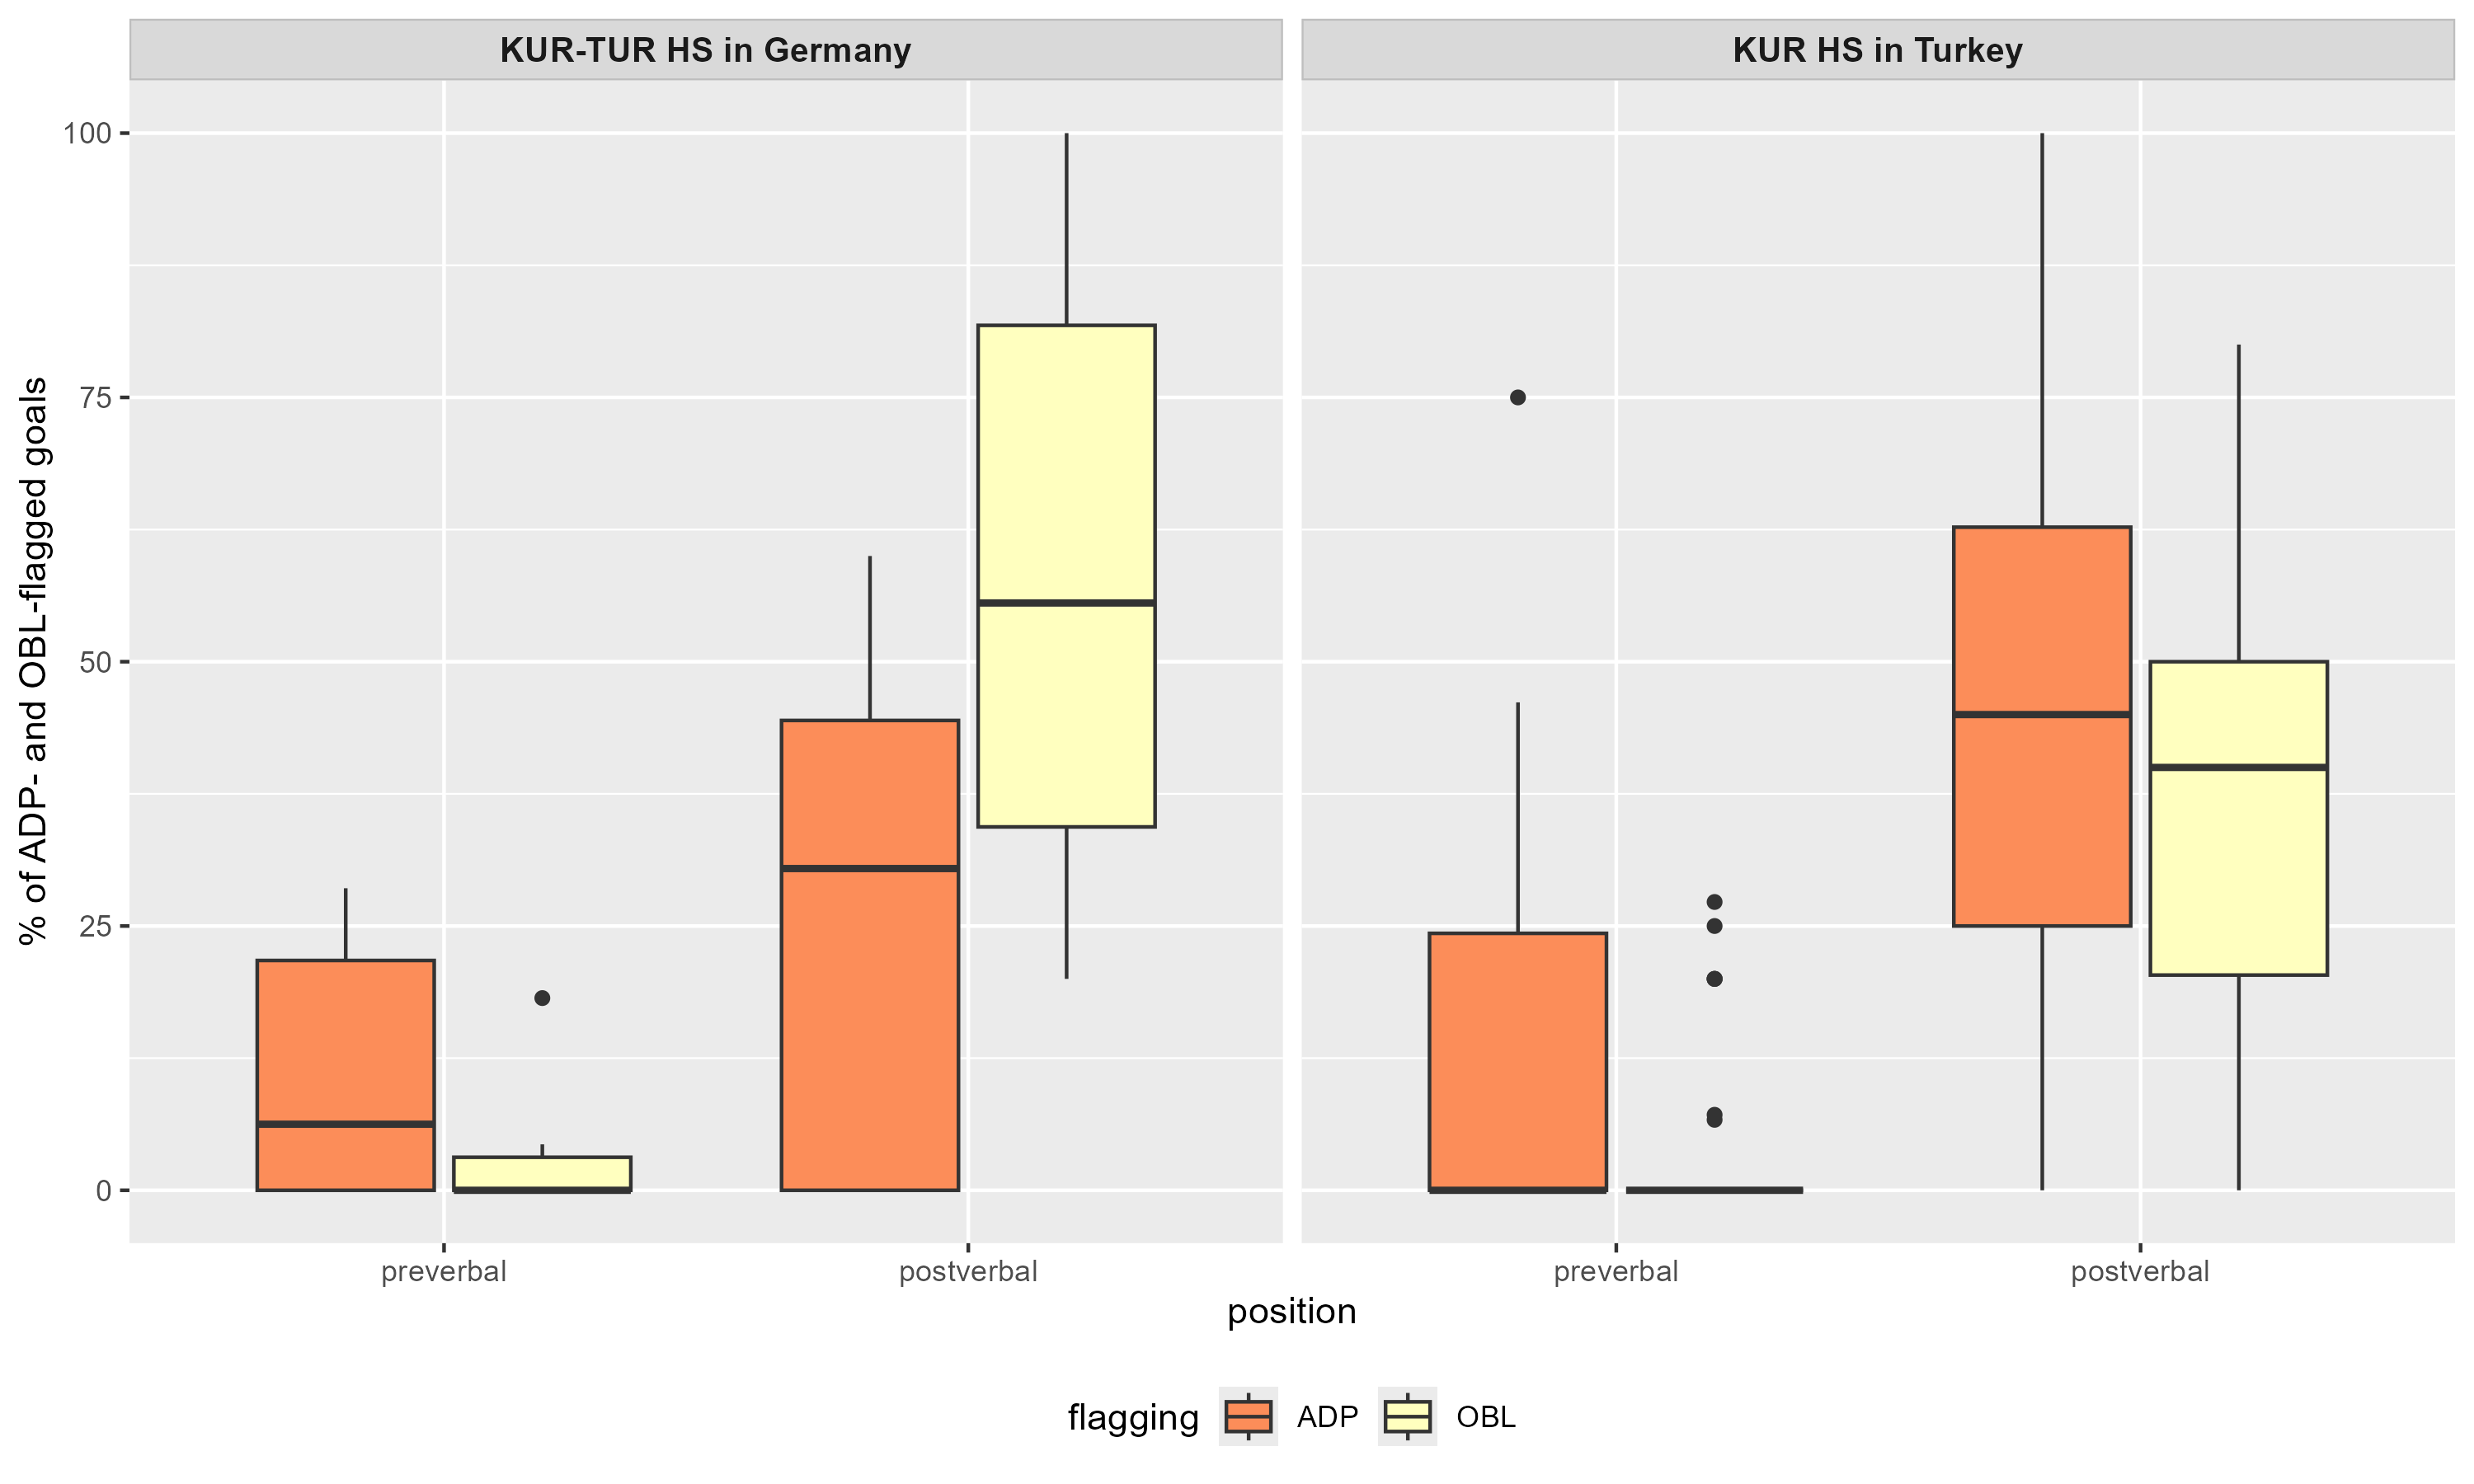
\includegraphics[width=\textwidth]{figures/iefremenko-img016.png}
\caption{\label{fig:key:17}Frequency distribution of goals of motion flagged with oblique case (OBL) or an adposition (ADP) in two country groups.}
\end{figure}

\newpage
\figref{fig:key:17} illustrates the frequency distribution of goals of motion, flagged with either the oblique case (OBL) or an adposition (ADP), and positioned in the pre- or post-predicate. The frequency of each type of flagging is calculated in relation to the total number of goals of motion within the data from each country group.

The figure shows that Kurmanji speakers in both countries use both types of flagging. Regarding the position of goals of motion, the post-predicate position is favored for both types of flagging among both speaker groups. In Germany, ADP-marked goals occur postverbally with $\bar{x}${=27.59\%} and preverbally with $\bar{x}$={11.28\%}, while OBL-marked goals occur postverbally with $\bar{x}$={58.28\%} and preverbally with $\bar{x}$={2.85\%}. In Turkey, ADP-marked goals appear postverbally with $\bar{x}$={46.66\%} and preverbally with $\bar{x}$={13.32\%}, and OBL-marked goals occur postverbally with $\bar{x}$={35.82\%} and preverbally with $\bar{x}$={4.20\%}. Taken together, these means indicate that in Germany, case flagging (OBL) is preferred overall, with $\bar{x}$={58.28\%} of goals flagged with case compared to $\bar{x}$={27.59\%} flagged with an adposition (ADP). Conversely, in Turkey, speakers favor adpositional flagging, with $\bar{x}$={46.66\%} of goals flagged with an adposition versus $\bar{x}$={35.82\%} flagged with case.


Since flagging is the factor influencing the placement of goals in Kurmanji, the following discussion will address the two types of flagging separately.

\subsubsection{Goals of motion flagged with case}\label{sec:key:6.3.1.1}

As stated in \sectref{sec:key:3.3}, case-flagged goals in Kurmanji are licensed in the post-predicate position (\citealt{Haig2014, Haig2018, Gundogdu2019}), and the data clearly show that they are predominantly used post-predicatively. For instance, in \REF{ex:key:55}, the goal argument \textit{tope} ‘to the ball’ is placed after the verb \textit{avêtin} ‘to throw’.

\ea%55
  \label{ex:key:55} Kurmanji, TUbi29MK\_isK \\
\gll Kûçik   xe     avêt-e       top-e \\
dog  oneself    throw.\textsc{pst.3sg}-\textsc{drct}  ball-\textsc{obl.f}\\
\glt ‘The dog threw itself to the ball’ 
  \z

However, the data indicate that Kurmanji speakers in both Turkey and Germany also place case-flagged goals in the pre-predicate position, as illustrated in examples \REF{ex:key:56} and \REF{ex:key:57}.

\ea%56
  \label{ex:key:56} Kurmanji,  TUbi18MK\_isK \\
\gll Ji   dest-ê     xwê   iii   sêv   erd-ê     ket\\
from  hand\textsc{-ez.m}   own  hm  apple   ground\textsc{-obl.m} fell.\textsc{pst.3sg}\\
\glt ‘Apple fell down from her hands on the ground’
  \z

\ea%57
  \label{ex:key:57} Kurmanji, TUbi10MK\_fsK \\
\gll {Gog   ewk   bû     iii ling-ê     merik-ê   ket}\\
ball  thing   be.\textsc{pst.3sg}  hm  {} foot-\textsc{ez.m}  man-\textsc{obl.m}  fell.\textsc{pst.3sg}\\
\glt ‘Ball well was hmm, fell to the man’s foot’  
  \z

In examples \REF{ex:key:56} and \REF{ex:key:57}, the goal arguments \textit{erdê} `on the ground' and \textit{lingê merikê} `on the man's foot' are positioned immediately before the predicate. Previous research on word order in Kurmanji (\citealt{Haig2014, Haig2018, Gundogdu2019}) classifies such constructions as non-canonical because goal arguments can only occupy the pre-predicate position if they are adpositionally flagged. For instance, including the preposition \textit{li} `in' before the goal arguments in examples \REF{ex:key:56} and \REF{ex:key:57} would render the sentences canonical, as demonstrated in examples \REF{ex:key:58} and \REF{ex:key:59}.

\ea
    \label{ex:key:58} Kurmanji, self-constructed \\
\gll * Ji   dest-ê     xwê   iii   sêv   li  erd-e     ket\\
{} from  hand-\textsc{ez.m}   own  hm   apple   in  ground\textsc{-obl.m} fell.\textsc{pst.3sg}\\
\glt \, ‘Apple fell down from her hands to the ground.’ 
    \z

\ea
    \label{ex:key:59} Kurmanji, self-constructed \\
\gll * Gog   ewk   bû     iii li  ling-ê     merik-ê      ket\\
{} ball  thing   be.\textsc{pst.3sg}  hm  {} in  foot-\textsc{ez.m}  man-\textsc{obl.m}  fell.\textsc{pst.3sg} \\
\glt \, ‘Ball well was hmm, fell to the man’s foot.’
    \z

If an argument is case-flagged, it should be positioned in the post-predicate location, as Kurmanji allows at most two case-flagged noun phrases (the subject and direct object) in the pre-predicate position (\citealt{Gundogdu2019}). Placing case-flagged goals immediately before the predicate may alter their intended meaning. Therefore, from a grammatical perspective, the case-flagged goals in examples  \REF{ex:key:58} and \REF{ex:key:59} can be interpreted as direct objects due to their placement in the pre-predicate position.

Although the absolute number of sentences featuring case-flagged goals in the pre-predicate position is relatively low, the data reveal that this placement is present in the speech of both groups. Specifically, there are 12 instances from the data of Kurmanji-Turkish bilinguals in Turkey, accounting for 4.20\% of all goals of motion in that group. In contrast, the data from Kurmanji-Turkish heritage speakers in Germany include four instances, representing 2.85\% of all goals of motion in that group.

A closer analysis of the examples from Kurmanji-Turkish bilinguals in Turkey reveals a consistent pattern in the use of verbs with case-flagged goal arguments in the pre-predicate position. Specifically, 11 out of the 12 instances of case-flagged goals in this preverbal position were used with the verb \textit{ketin} ‘to fall,’ as shown in example \REF{ex:key:56} and \REF{ex:key:57}, while one instance was used with the verb \textit{firîn} ‘to fly.’

Furthermore, the examples with the verb \textit{ketin} ‘to fall’ can be categorized into two groups: those featuring body parts as arguments (\textit{dest} ‘hand’ or \textit{ling} ‘foot’) and those where the argument is the goal \textit{erd} ‘ground.’ The first group includes six instances, where the examples suggest that the ball falls into the man's hands or feet. However, the video shows that the ball falls from the man's hands onto the road. This implies that the preposition \textit{ji} ‘from’ may be omitted or reduced, indicating that the constituents in the pre-predicate position are not actually goals but rather sources of motion, as shown in example \REF{ex:key:60}. Similarly, the example with the verb \textit{firîn} ‘to fly’ also includes the argument \textit{dest} ‘hand’ in the pre-predicate position. These instances, which can be interpreted as sources of motion, further explain their noncanonical placement before the verb, as sources of motion in Kurmanji are typically positioned in the preverbal position.

\ea
  \label{ex:key:60} Kurmanji, Tubi09MK\_iwK \\
     \gll Nişkava   gog   dest-ê     wî   ket \\
suddenly  ball  hand-\textsc{ez.m}  her  fall.\textsc{pst.3sg}\\
\glt ‘Suddenly the ball fell from his hands’ 
  \z

Example \REF{ex:key:60} is a written instance from a Kurmanji speaker in Turkey, where the argument \textit{destê wî} ‘her hand’ actually implies a source of action, suggesting that the preposition \textit{ji} ‘from’ has been omitted. Omitting a preposition is a phenomenon sometimes observed in the data of Kurmanji-Turkish bilinguals in Turkey. For instance, in \REF{ex:key:61}, the verb \textit{vegerandin} ‘to return’ implies motion away from a source. Therefore, the locative noun phrase is expected to be marked as a source of motion, not as a goal, as in the example.

\ea
  \label{ex:key:61} Kurmanji, TUbi04MK\_fwK \\
\gll Dema    ez     zanîngeh-ê          ve-di-geriya-m\\
while    I      university\textsc{-obl.f}     \textsc{prfx-prs-}return-\textsc{1sg}\\
\glt ‘While I was coming back (from) the college…’ 
  \z

The tendency to omit prepositions may arise from convergence effects with the majority language, Turkish, which does not use prepositions in the same way. This phenomenon is similarly observed in Turkish child heritage speakers in Germany \citep{Turgay2010} and in L1 Turkish learners of English and German (\citealt{Ozisik2014, Yildiz2016}). These studies indicate that L1 Turkish speakers often omit prepositions when using their L2, whether it be German or English, both of which are prepositional languages. In contrast to these findings, example \REF{ex:key:61} suggests a possible influence of L2 Turkish on the use of L1 Kurmanji.

Considering the six examples with the verb \textit{ketin} ‘to fall’ that feature a body part as instances of the source of motion, there are five remaining examples with the case-flagged goal \textit{erdê} ‘onto the ground’ placed before the verb \textit{ketin} ‘to fall.’ It is important to note that this construction is only found in the data from Kurmanji-Turkish bilinguals in Turkey. In Turkish, \textit{erdê ketin} is expressed as \textit{yere düşmek}, which translates literally to ‘to fall on the ground.’ This expression is a fixed construction in Turkish, where \textit{yer-e} (ground-\textsc{dat}) in \textit{yere düşmek} (ground-\textsc{dat} fall.\textsc{inf}) cannot be placed in the post-predicate position and is always directly attached to the verb. This observation is corroborated by the RUEG data, a search for the construction \textit{yere düşmek} revealed that all instances occur in the immediate pre-predicate position. This result is based on ten occurrences of the construction in the Turkish of Kurmanji-Turkish bilingual speakers, eight instances of \textit{yere düşmek} in Kurmanji-Turkish heritage speakers in Germany \citep{IefremenkoEtAl2024}, and 19 occurrences in the Turkish of monolingual speakers \citep{LudelingEtAl2024}. Thus, the noncanonical position of the argument \textit{erdê} in Kurmanji may be attributed to the direct copying of the entire construction from Turkish. This finding will be further discussed in \sectref{sec:key:7.1}.

However, beyond the cross-linguistic explanation, the noncanonical position may also be influenced by the verb \textit{ketin} itself. In Kurmanji, there are constructions where \textit{ketin} functions as a light verb, lacking its full meaning, as seen in phrases like \textit{bi rê ketin} ‘to set off (on a journey)’ and \textit{li ber ketin} ‘to meet/to encounter.’ This could account for the higher frequency of construction copying observed with the verb \textit{ketin}, although it does not fully explain the noncanonical position of the case-flagged goal \textit{erdê}.

Additionally, it is essential to note that the noncanonical construction with a goal argument in the pre-predicate position does not dominate in Kurmanji usage. Most speakers still place case-flagged goals, including \textit{erdê}, in the post-predicate position. In the Kurmanji data from heritage speakers in Turkey, the construction ‘to fall on the ground’ has been used 20 times, with 15 instances being canonical (featuring a postposed argument) and five instances being noncanonical (with the argument in the pre-predicate position). Furthermore, even speakers who occasionally place the argument \textit{erdê} in the pre-predicate position in one communicative situation employ the canonical post-predicate position in other communicative situaitions. For instance, one female speaker placed the goal \textit{erdê} in the immediate pre-predicate position during the informal spoken production (see example \REF{ex:key:62}) but used it in the canonical post-predicate position in the written mode (see example \REF{ex:key:63}).

\ea \label{ex:key:62} Kurmanji, TUbi19FK\_isK \\
\gll Pişte    zilam   iii   gok-ê    xwe imm (--)   ji   dest-ê     xwa\\
afterwards  man  hm  ball-\textsc{ez.f}  \textsc{refl}  hmm  {} from  hand\textsc{-ez.m}  \textsc{refl} \\
\gll imm (--)   erd-ê       ket \\
hmm   {} ground-\textsc{obl.m}    fall.\textsc{pst.3sg}\\
\glt ‘Afterwards the man hmm his ball hmm (--) fell from his hand hmm (--) to the ground.’ 
\z


\ea
  \label{ex:key:63} Kurmanji, TUbi19FK\_iwK \\
\gll Gok-ê     zîlam   ji   dest-e    wî   ket     ard-ê \\
ball-\textsc{obl.f}  man  from  hand\textsc{-ez.m}  his  fall.\textsc{pst.3sg}  ground-\textsc{obl.m}\\
\glt ‘The man's ball fell from his hand onto the ground.’ 
  \z

Regarding the Kurmanji speakers in Germany, the relatively low absolute number of noncanonically placed arguments may be attributed to the fact that the data come from only nine speakers, resulting in fewer instances compared to Kurmanji-Turkish speakers in Turkey. Specifically, there are four case-flagged goals positioned pre-predicatively, produced by three speakers. Interestingly, unlike the Kurmanji speakers in Turkey, there is greater variation in the verbs that accommodate case-flagged arguments in the preverbal position among the speakers in Germany. These speakers employ pre-predicate goals with a range of verbs, including \textit{xistin} ‘to hit,’ \textit{lêxistin} ‘to beat/to hit,’ \textit{bazdan} ‘to run,’ and \textit{kirin} ‘to do.’

Examining these examples more closely reveals that two instances originate from the same speaker and exhibit code-switching from Turkish to Kurmanji. In these sentences, the goal is expressed in Turkish, while the verb is in Kurmanji (see examples \REF{ex:key:64} and \REF{ex:key:65}). Notably, the goal argument is a cognate of the Turkish word for ‘car’ (\textit{araba}), leading to ambiguity regarding whether the argument is in Kurmanji or Turkish. However, given that the data is written, the participant’s spelling suggests that the argument is the Turkish noun \textit{araba}. Consequently, the pre-predicative placement of the goal argument in examples \REF{ex:key:64} and \REF{ex:key:65} may be influenced by the Turkish structure of the utterance, with only the verb being in Kurmanji. From the perspective of canonical Turkish, placing a goal constituent in the pre-predicate position is a normative practice.

\ea \label{ex:key:64} Kurmanji, TUbi06MK\_fwK \\
\gll Alışveriş-e   araba-ya   di-kin  \\
grocery-\textsc{obl}  car-\textsc{dat}  \textsc{prs}-do\textsc{.3sg}\\
\glt ‘She was putting groceries into the car.’ 
\z

\ea
  \label{ex:key:65} Kurmanji and Turkish, TUbi06MK\_fwK \\
     \gll Arka-daki   araba   da   ön-deki   araba-ya   lexe \\
back\textsc{-attr}  car  also  front-\textsc{attr}  car-\textsc{dat}  bump\textsc{.pst.3sg}\\
\glt ‘The car at the back hit the car at the front.’ 
  \z

Thus, only two examples remain: in one instance, the verb \textit{bazdan} ‘to run’ takes a pre-predicative goal argument (see example \REF{ex:key:66}), while in the other, the verb \textit{xistin} ‘to hit’ features a goal argument in the pre-predicate position (see example \REF{ex:key:67}).

\ea
  \label{ex:key:66} Kurmanji, TUbi01FK\_isK \\
     \gll Zilam   pêşi-yê   bazda\\
man  front-\textsc{obl}  run\textsc{.pst.3sg}    \\
\glt ‘The man ran ahead.’ 
  \z

\ea
  \label{ex:key:67} Kurmanji, TUbi03FK\_isK \\
\gll Jî  ereba  pêşi-yê    xist\\
also  car  front-\textsc{obl}  hit.\textsc{pst.3sg}\\
\glt ‘He also hit the front car.’ 
  \z

Thus, the analysis revealed that in Kurmanji heritage speakers in Germany, there are only two instances of case-flagged goals placed in the noncanonical pre-predicate position. Furthermore, unlike in the cases observed among Kurmanji-Turkish bilinguals in Turkey, there is no specific verb or construction that prompts this noncanonical argument placement. This finding will be further explored in \sectref{sec:key:7.1}.

\subsubsection{Adpositional goals of motion}

As discussed in \sectref{sec:key:6.3.1}, both groups in the data show a preference for using adpositional goals in the post-predicate position rather than in the pre-predicate position. Previous studies by \citet{Haig2014} and \citet{Gundogdu2019} also indicate that adpositional goals predominantly appear post-predicate, though their placement can vary depending on the type of adposition and the dialect.

The following section presents the results of the frequency analysis for goals of motion flagged by different types of adpositions, calculated in relation to the total number of adpositional goals of motion within each speaker group (see \figref{fig:key:18}). For this analysis, five types of adpositionally flagged goals are categorized: those flagged by a basic preposition, those flagged with a locational noun, those that combine a basic preposition with a locational noun, those flagged by a postposition, and those flagged by a circumposition.

\begin{figure}
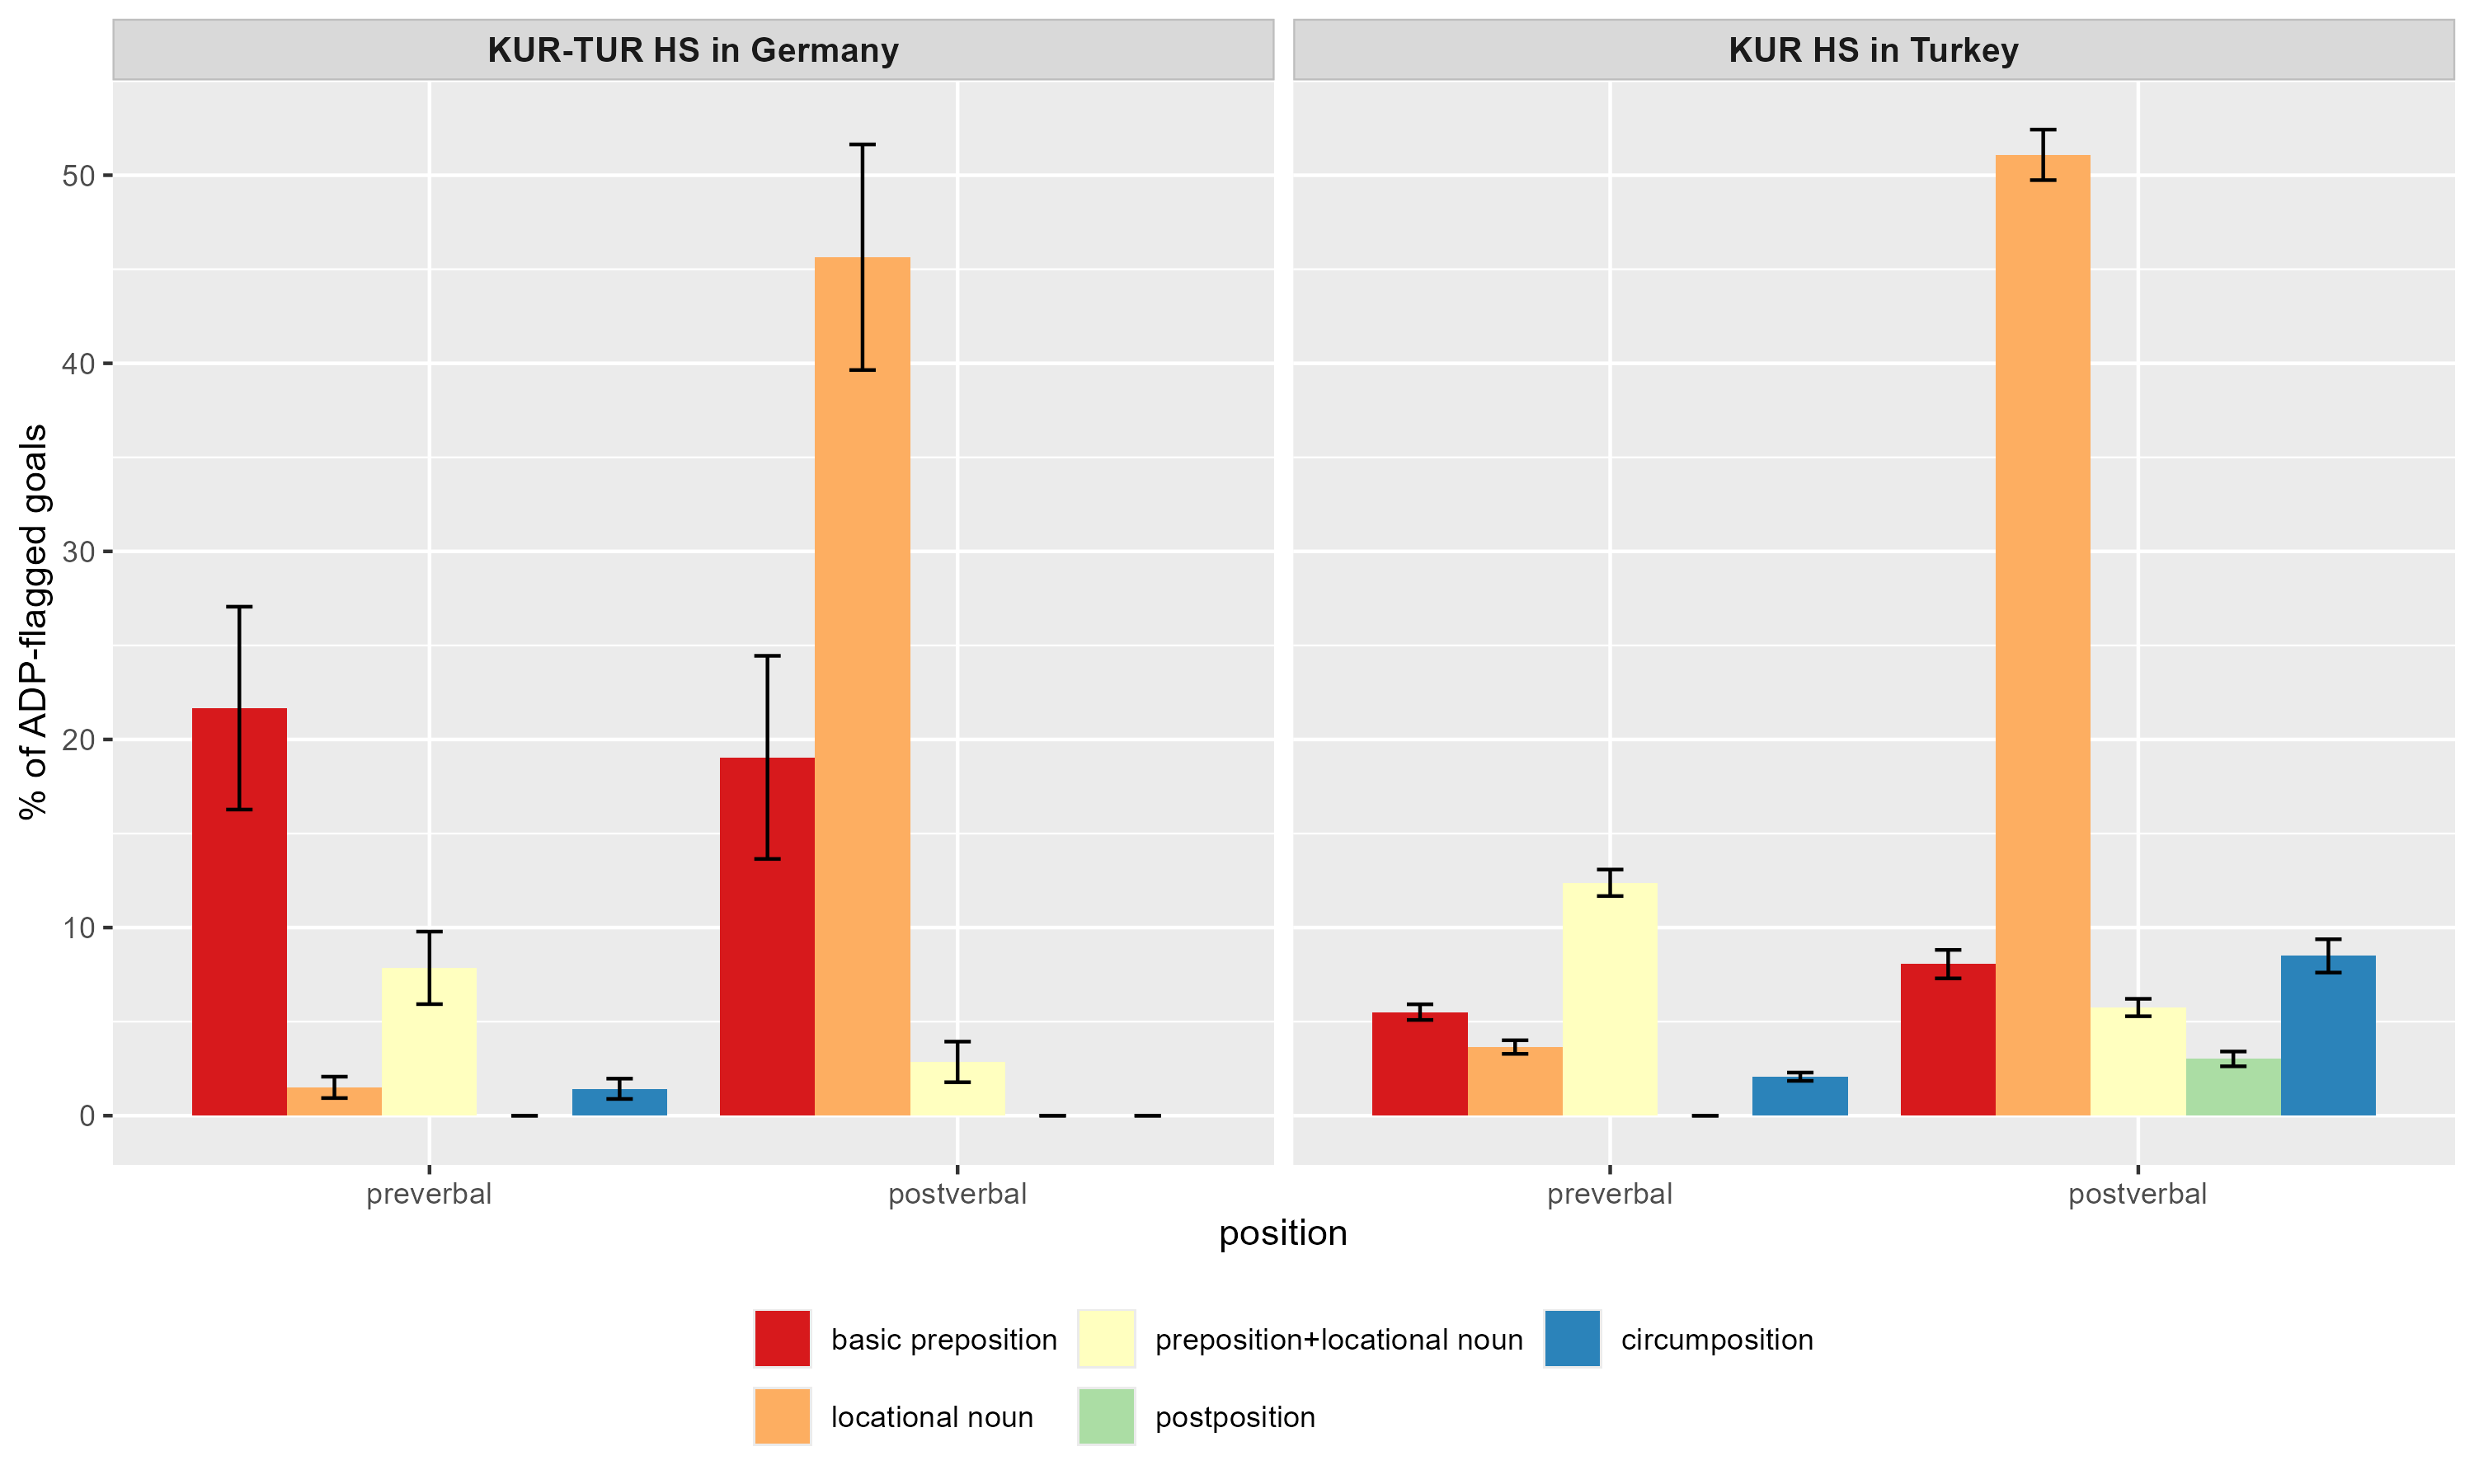
\includegraphics[width=\textwidth]{figures/iefremenko-img017.png}
\caption{\label{fig:key:18}Frequency of goals of motion flagged with different types of adpositions.}

\end{figure}

\figref{fig:key:18} illustrates the frequency distribution of goals of motion flagged by different types of adpositions, relative to the total number of adpositional goals of motion within each speaker group. Error bars represent standard error to enhance the precision of the mean estimates, particularly since some adposition types have low absolute counts.

Notably, \figref{fig:key:18} indicates that Kurmanji speakers predominantly use locational nouns as adpositions to express goals of motion. When combining occurrences in both post- and pre-predicate positions, 54.73\% of adpositional goals in Turkey and 47.14\% in Germany are flagged by locational nouns. As highlighted in \sectref{sec:key:3.3.1}, goals flagged with locational nouns are consistently placed in the post-predicate position because they are grammaticalized nouns. While the data primarily show that these goals are placed post-predicatively, there are some instances in both groups where such goals appear in the pre-predicate position.

\tabref{tab:key:12turkey} and \tabref{tab:key:12germany} present the absolute numbers of the different types of adpositions used in either the pre- or post-predicate position within the data.

% {\small
% \begin{longtable}
% {l p{2cm} l@{}r r }
% \caption{\label{tab:key:12turkey}The absolute number of different types of adpositions in the pre- and post-predicate position in the Turkey data.}\\
% \lsptoprule
% Group & Adposition type & Name & Pre-predicate & Post-predicate\\
% \midrule
% \endfirsthead
%
% \lsptoprule
%  Group & Adposition type & Name & Pre-predicate & Post-predicate\\
% \midrule
% \endhead
%
% \lspbottomrule
% \endlastfoot
%
% \tablevspace
% Kurmanji & \multirow{3}{2cm}{Basic prepositions} & \textit{bo} ‘to’ & 0 & 2\\
% HS in &  & \textit{li} ‘in’ & 12 & 3\\
% Turkey &  & \textit{pê} ‘to/into’ & 0 & 1\\
% \tablevspace
% \cline{2-5}
% \tablevspace
% \quad & \multirow{8}{2cm}{Locational nouns} & \textit{ber} ‘front’ & 1 & 14\\
% \quad &  & \textit{bin} ‘below’ & 0 & 2\\
% \quad &  & \textit{cem} ‘to’ & 0 & 5\\
% \quad &  & \textit{hemberî} ‘opposite’ & 4 & 4\\
% \quad &  & \textit{hinda} ‘side’ & 0 & 1\\
% \quad &  & \textit{nav / nava} ‘middle’ & 0 & 20\\
% \quad &  & \textit{peşiya} ‘front’ & 0 & 12\\
% \quad &  & \textit{ser} ‘over’ & 0 & 17\\
% \tablevspace
% \cline{2-5}
% \tablevspace
% \quad & \multirow{9}{2cm}{Preposition + loc. Noun} & \textit{ber bi} ‘towards’ & 10 & 10\\
% \quad &  & \textit{bi ber} ‘towards’ & 0 & 2\\
% \quad &  & \textit{bi ser} ‘ahead’ & 1 & 0\\
% \quad &  & \textit{li hemberi} ‘towards’ & 1 & 0\\
% \quad &  & \textit{li nav} ‘in’ & 2 & 0\\
% \quad &  & \textit{li pey} ‘after’ & 1 & 1\\
% \quad &  & \textit{li piştê} ‘behind’ & 2 & 0\\
% \quad &  & \textit{li ser} ‘on’ & 0 & 6\\
% \tablevspace
% \cline{2-5}
% \tablevspace
% \quad & \multirow{2}{2cm}{Postpositions} & \textit{…da} ‘in’ & 0 & 3\\
% \quad &  & \textit{…ve} & 0 & 1\\
% \tablevspace
% \cline{2-5}
% \tablevspace
% \quad & \multirow{7}{2cm}{Circumpositions} & \textit{ber bi…da} ‘towards’ & 1 & 0\\
% \quad &  & \textit{ber…de} ‘in front of’ & 0 & 1\\
% \quad &  & \textit{ber bi…ve} 'towards' & 3 & 1\\
% \quad &  & \textit{ber…de} 'in front of' & 0 & 1\\
% \quad &  & \textit{ber…ve} 'towards' & 1 & 1\\
% \quad &  & \textit{bi…de} 'towards' & 0 & 1\\
% \tablevspace
% \quad &  & \textit{li…da} ‘at/in’ & 1 & 2\\
% \quad &  & \textit{orta…da} ‘in the middle of’ & 0 & 1\\
% \tablevspace
% \midrule
%
% \lspbottomrule
%
% \tablevspace
% Kurmanji- & \multirow{2}{2cm}{Basic prepositions} & \textit{bo} 'to' & 0 & 4\\
% Turkish HS &  & \textit{li} 'in' & 7 & 1\\
% in Germany & \quad & \quad & \quad \\
% \cline{2-5}
% \tablevspace
% \quad & \multirow{8}{2cm}{Locational nouns} & \textit{ber} 'in front of / towards' & 1 & 6\\
% \quad &  & \textit{bin} 'under' & 0 & 1\\
% \quad &  & \textit{cem} 'to' & 0 & 15\\
% \quad &  & \textit{hindir} 'inside' & 0 & 1  \\
% \quad &  & \textit{peşiya} 'in front of' & 0 & 2\\
% \quad &  & \textit{piş} 'behind' & 0 & 1\\
% \quad &  & \textit{ser} 'on' & 0 & 7\\
% \tablevspace
% \cline{2-5}
% \tablevspace
% \quad & \multirow{3}{2cm}{Preposition+loc. Noun} & \textit{li ber} 'in front of/ before' & 1 & 0\\
% \quad &  & \textit{li pey} 'after' & 2 & 1\\
% \quad &  & \textit{li ser} 'on/ on top of' & 2 & 1\\
% \tablevspace
% \cline{2-5}
% \tablevspace
% & Circumposition & \textit{ber bi…ve} ‘towards’ & 1 & 0\\
% \tablevspace
% \end{longtable}
% }

\begin{table}[t]\small
\caption{\label{tab:key:12turkey}The absolute number of different types of adpositions in the pre- and post-predicate position (Kurmanji HS in Turkey).}
\begin{tabularx}{\textwidth}{@{}l@{}   Q l@{}r r }
\lsptoprule
 & Adposition type & Name & Pre-predicate & Post-predicate\\
\midrule
  & \multirow{3}{2cm}{Basic prepositions} & \textit{bo} ‘to’ & 0 & 2\\
  &  & \textit{li} ‘in’ & 12 & 3\\
  &  & \textit{pê} ‘to/into’ & 0 & 1\\
% \tablevspace
\midrule % \cline{2-5}
% \tablevspace
 & \multirow{8}{2cm}{Locational nouns} & \textit{ber} ‘front’ & 1 & 14\\
 &  & \textit{bin} ‘below’ & 0 & 2\\
 &  & \textit{cem} ‘to’ & 0 & 5\\
 &  & \textit{hemberî} ‘opposite’ & 4 & 4\\
 &  & \textit{hinda} ‘side’ & 0 & 1\\
 &  & \textit{nav / nava} ‘middle’ & 0 & 20\\
 &  & \textit{peşiya} ‘front’ & 0 & 12\\
 &  & \textit{ser} ‘over’ & 0 & 17\\
% \tablevspace
\midrule % \cline{2-5}
% \tablevspace
 & \multirow{9}{2cm}{Preposition + loc. Noun} & \textit{ber bi} ‘towards’ & 10 & 10\\
 &  & \textit{bi ber} ‘towards’ & 0 & 2\\
 &  & \textit{bi ser} ‘ahead’ & 1 & 0\\
 &  & \textit{li hemberi} ‘towards’ & 1 & 0\\
 &  & \textit{li nav} ‘in’ & 2 & 0\\
 &  & \textit{li pey} ‘after’ & 1 & 1\\
 &  & \textit{li piştê} ‘behind’ & 2 & 0\\
 &  & \textit{li ser} ‘on’ & 0 & 6\\
% \tablevspace
\midrule %\cline{2-5}
% \tablevspace
 & \multirow{2}{2cm}{Postpositions} & \textit{…da} ‘in’ & 0 & 3\\
 &  & \textit{…ve} ‘towards?’ & 0 & 1\\
% \tablevspace
\midrule %\cline{2-5}
% \tablevspace
 & \multirow{7}{2cm}{Circumpositions} & \textit{ber bi…da} ‘towards’ & 1 & 0\\
 &  & \textit{ber…de} ‘in front of’ & 0 & 1\\
 &  & \textit{ber bi…ve} 'towards' & 3 & 1\\
 &  & \textit{ber…de} 'in front of' & 0 & 1\\
 &  & \textit{ber…ve} 'towards' & 1 & 1\\
 &  & \textit{bi…de} 'towards' & 0 & 1\\
% \tablevspace
 &  & \textit{li…da} 'at/in' & 1 & 2\\
 &  & \textit{orta…da} 'in the middle of' & 0 & 1\\
\lspbottomrule
\end{tabularx}
\end{table}

\begin{table}\small
\caption{\label{tab:key:12germany}The absolute number of different types of adpositions in the pre- and post-predicate position (Kurmanji-Turkish HS in Germany)}
\begin{tabularx}{\textwidth}{@{}l@{} Q l@{}r r }
\lsptoprule
& Adposition Type & Name & Pre-predicate & Post-predicate\\
\midrule
& {Basic prepositions} & \textit{bo} 'to' & 0 & 4\\
 &  & \textit{li} 'in' & 7 & 1\\
\midrule %\cline{2-5}
% \tablevspace
 & \multirow{8}{2cm}{Locational nouns} & \textit{ber} 'in front of / towards' & 1 & 6\\
 &  & \textit{bin} 'under' & 0 & 1\\
 &  & \textit{cem} 'to' & 0 & 15\\
 &  & \textit{hindir} 'inside' & 0 & 1  \\
 &  & \textit{peşiya} 'in front of' & 0 & 2\\
 &  & \textit{piş} 'behind' & 0 & 1\\
 &  & \textit{ser} 'on' & 0 & 7\\
% \tablevspace
\midrule %\cmidrule(lr){2-5}
% \tablevspace
 & \multirow{3}{2cm}{Preposition+loc. Noun} & \textit{li ber} 'in front of/ before' & 1 & 0\\
 &  & \textit{li pey} 'after' & 2 & 1\\
 &  & \textit{li ser} 'on/ on top of' & 2 & 1\\
% \tablevspace
\midrule %\cmidrule{2-5}
% \tablevspace
& Circumposition & \textit{ber bi…ve} 'towards' & 1 & 0\\
\lspbottomrule
\end{tabularx}
\end{table}

\largerpage
\tabref{tab:key:12turkey} shows that goals flagged with locational nouns such as \textit{hemberî} ‘opposite’ and \textit{ber} ‘front’ (a total of five examples) are placed in the pre-predicate position by Kurmanji speakers in Turkey (example \REF{ex:key:68}). Similarly, speakers in Germany use \textit{ber} ‘front’ in the pre-predicate position, with one documented example (see example \REF{ex:key:69}).

 \ea \label{ex:key:68} Kurmanji, TUbi07FK\_isK \\
\gll Mirov-ê  hemberî  rê  revî \\
man\textsc{-obl.m} across    road  run.\textsc{pst.3sg}\\
\glt ‘The man ran across the road’ 
\z

\ea
  \label{ex:key:69} Kurmanji, DEtr01FK\_iwK \\
\gll Kûçik   ber     erebê   {dihat   diçû}\\
dog  towards  car  was\_coming\\
\glt ‘The dog was coming towards the car’
  \z

Interestingly, in the Kurmanji data from Turkey four out of five examples of preverbal arguments flagged with a locational noun appear in the construction \textit{hemberî rê} ‘across the road’ with the verbs \textit{revîn} ‘to run’ and \textit{çûn} ‘to go’. As for the data from Germany, there is only one construction with a preverbal goal argument flagged with the help of a locational noun \textit{ber} ‘front’. In fact, this example comes from the speaker who also placed a case-flagged goal in the pre-predicate position (see example \REF{ex:key:67}).

The next most common type of flagging observed in the data involves basic prepositions, including \textit{bo} ‘to/for,’ \textit{li} ‘in,’ and a single instance of \textit{pê} ‘to/into.’ Analysis reveals that goals flagged with these basic prepositions in Kurmanji appear in both pre- and post-predicative positions. However, a notable trend emerges: the preposition \textit{bo} ‘to/for’ tends to be used in the post-predicate position, while \textit{li} ‘in’ is more frequently found in the pre-predicate position (see \tabref{tab:key:12turkey}). The following examples illustrate the use of the preposition \textit{li} in both the pre- \REF{ex:key:70} and post-predicate positions \REF{ex:key:71}.

\ea
  \label{ex:key:70} Kurmanji, TUbi10MK\_isK \\
     \gll Ew   gog   li   erd-ê     ket\\
that  ball  in  ground\textsc{-obl.m}  fall.\textsc{pst.3sg}  \\
\glt ‘That ball fell onto the ground.’ 
  \z

\ea
  \label{ex:key:71} Kurmanji, TUbi12MK\_iwK \\
     \gll Ket     li   erebe-ya   pêşî\\
fall.\textsc{pst.3sg}  in  car-\textsc{ez.f}  front\\
\glt ‘It bumped into the front car.’ 
  \z

It should also be noted that the preposition \textit{li} is commonly used to indicate location, in which case it typically appears in the pre-predicate position. This polysemy may account for its frequent use in the pre-predicate position even when indicating goals.

The next type of adposition is basic prepositions used in combination with locational nouns. The data indicate that the positioning of these forms is flexible, as they appear almost equally in both pre- and post-predicate positions across both speaker groups (see examples \REF{ex:key:72} and \REF{ex:key:73}). Although, for Kurmanji-Turkish heritage speakers in Germany, the number of instances featuring a basic preposition combined with a locational noun is relatively low, totaling only seven examples.

\ea
  \label{ex:key:72} Kurmanji, TUbi05MK\_fwK \\
\gll Du   erebe   {li pey hev}     {ber bi}     jinik-ê     di-hat-in \\
two  car  one\_after\_the\_other  towards  woman-\textsc{obl.f}  \textsc{prs}-come-\textsc{3pl}\\
\glt ‘Two cars were coming towards the woman one after the other.’ 
  \z

\ea
  \label{ex:key:73} Kurmanji, TUbi29MK\_isK \\
     \gll Erebe   jî   di-hat-e     {ber bi}     kûçik-ê \\
car  also  \textsc{prs}-come-\textsc{drct}  towards {}  dog-\textsc{obl.m}\\
\glt ‘The car was coming towards the dog.’ 
  \z

The least frequent type of adpositional goal in the data consists of adpositional phrases that incorporate postpositional particles, specifically postpositions and circumpositions. The positioning of these arguments also exhibits variation. Postpositions are exclusively found in the post-predicate position and only within the data from speakers in Turkey (see example \ref{ex:key:74}). In contrast, circumpositions display more flexibility, occurring in both pre- and post-predicate positions (see examples \ref{ex:key:75} and \ref{ex:key:76}). Notably, there is only one instance of a circumposition in the data from Germany.

\ea
  \label{ex:key:74} Kurmanji, TUbi09MK\_fsK \\
\gll Jinik-ek   ereba   xwe   da   hinek   {tişt mişt}   di-xist-in   erebê   de\\
woman-\textsc{indf}  car  \textsc{refl}  \textsc{post}  some  things \textsc{prs-}place-\textsc{3pl}  car  \textsc{post}\\
\glt ‘A woman was putting some things in her car.’ 
  \z

\ea
  \label{ex:key:75} Kurmanji, TUbi04MK\_fwK \\
\gll û   ew   gog   ji   dest-ê     wî   revî \\
and  that  ball  from  hand\textsc{-ez}  his  escape\textsc{.pst.3sg}\\
\gll {ber bi}     cadde-yê   ve\\
towards  street-\textsc{obl}  \textsc{post}  \\
\glt ‘And the ball ran from his hands to the street.’ 
  \z
  
\ea%
  \label{ex:key:76} Kurmanji, TUbi15MK\_fsK \\
\gll {Ji nîşka va}   e   {ber bi}     top-ê     va   bazda  \\
all\_of\_a\_sudden   hm  towards ball\textsc{-obl}  \textsc{post}  run\textsc{.pst.3sg}\\
\glt ‘All of a sudden it ran to the ball.’  
  \z

Furthermore, \tabref{tab:key:12turkey} and \ref{tab:key:12germany} highlight qualitative differences in the use of adpositional goals between the country groups. While speakers in Turkey use a variety of adpositions, those in Germany primarily rely on basic prepositions and locational nouns, particularly the locational noun \textit{cem} ‘to’. Speakers in Germany tend to avoid postpositions and circumpositions, indicating a preference for adpositions that consist of one or two elements at most. However, it is important to note that the data set from Germany is based on only nine speakers, suggesting that collecting additional data from this group could introduce greater variability in the types of adpositions used.

In summary, the analysis of goal placement indicates that goals flagged with an adposition in Kurmanji can occur in both pre- and post-predicate positions. This applies to goal arguments flagged with all types of adpositions, with the exception of locational nouns. Previous research (\citealt{Haig2014}, \citealt{HaigThiele2014}) suggests that locational nouns historically evolved from nouns and are thus licensed in the post-predicate position alongside case-flagged goals. While the data predominantly show that the placement of locational nouns and case-flagged goals is post-predicative, there are instances where these goals appear in the pre-predicate position. Due to these differing placement preferences, locational nouns and case-flagged goals will be discussed separately from other types of adpositions in the following analyses.

\subsection{Exploring possible factors influencing the position of goals of (caused) motion flagged with case or a locational noun in Kurmanji}\label{sec:key:6.3.2}

This section focuses on two potential factors that influence the position of goals in (caused) motion in Kurmanji. First, it explores the effect of the speakers' majority language, specifically whether there are differences between the groups in Turkey and Germany. However, as shown in the findings presented in \sectref{sec:key:6.3.1}, this factor does not seem to have an impact on the position of goals. Furthermore, the effect of communicative situations, i.e., formality and mode, will be discussed. These factors remain underexplored in Kurmanji, primarily due to the limited exposure of Kurmanji speakers to different registers of the language.

Finally, although not an initial goal of the study, the possible effects of information structure on the placement of goals of motion will be examined. \citet{Asadpour2021} found that in Mukri Kurdish spoken in Iran, information structure plays a particularly significant role in the use of the post-predicate position. Therefore, this factor will be investigated in Kurmanji as well.

\subsubsection{The effect of the speaker group on the position of goals of (caused) motion flagged with case or a locational noun}\label{sec:key:6.3.2.1}

As mentioned in \sectref{sec:key:6.3.1}, both speaker groups prefer the post-predicate position for both types of flagging. However, both groups also tend to place case-flagged goals and locational nouns noncanoncanically, namely, in the pre-predicate position.

To statistically assess whether the speaker group influences the use of case-flagged goals in the pre-predicate position, a generalized logistic mixed-effects model was conducted. The model followed a binomial distribution. Position (preverbal coded as 1, postverbal coded as 0) served as the dependent variable, while Group (Kurmanji speakers in Turkey (Tubi) and Kurmanji speakers in Germany (Debi)) was included as a fixed effect. Participant was included as a random variable. The results of the regression analysis are presented in \tabref{tab:key:13}.

\begin{table}

\begin{tabularx}{\textwidth}{XYY}
\lsptoprule
\textbf{Random effects:}\\
\midrule
% \lsptoprule
\textbf{Groups} & \textbf{Variance} & \textbf{Standard} \textbf{Deviation}\\
Participant (Intercept) & 0.43 & 0.65\\
% \lspbottomrule
\midrule
\end{tabularx}

\begin{tabularx}{\textwidth}{Xrrrr}
% \lsptoprule
\textbf{Fixed effects:} & & \\
\midrule
\textbf{Fixed effect} & \textbf{Estimate} & \textbf{Std. Error} & \textbf{z-value}  & \textbf{\textit{p}-value}\\
Intercept & {}-2.99 & 0.59 & {}-5.05 & $<.0001^{***}$\\
Group (Tubi) & 0.49 & 0.59 & 0.83 & .40\\
\lspbottomrule
\end{tabularx}
\caption{\label{tab:key:13}Regression table for glmer with the dependent variable Position and the independent variable Group.}
\end{table}

The generalized logistic mixed-effects model showed no significant effect of Group on Position, indicating that speaker group does not significantly influence the placement of case-flagged goals and goals flagged with locational noun. Random effects analysis revealed moderate variation across participants.

\subsubsection{The effect of formality and mode on the position of goals flagged with case or a locational noun}\label{sec:key:6.3.2.2}

According to previous research on word order in Kurmanji (\citealt{Haig2014, Gundogdu2019}), the position of locational nouns and case-flagged goals is generally fixed in the post-predicate position. However, some speakers in the dataset also use these goals in the pre-predicate position. To determine whether the controlled variables—formality and mode—affect the placement of these two types, a binomial generalized linear mixed-effects model was conducted. The dependent variable was Position of Goals Flagged with Case or a Locational Noun (post-predicate (0) vs. pre-predicate (1), while Formality (formal vs. informal) and Mode (spoken vs. written) served as independent variables. The model also accounted for individual variation in the speakers by including Participant as a random variable. \tabref{tab:key:14} provides an overview of the regression results.

\begin{table}
\begin{tabularx}{\textwidth}{XYY}
\lsptoprule
\textbf{Random effects:}\\
\midrule
% \lsptoprule
\textbf{Groups} & \textbf{Variance} & \textbf{Standard} \textbf{Deviation}\\
Participant (Intercept) & 0.52 & 0.72\\
% \lspbottomrule
\midrule
\end{tabularx}

\begin{tabularx}{\textwidth}{Xrrrr}
% \lsptoprule
\textbf{Fixed effects:} & & & & \\
\midrule
\textbf{Fixed} \textbf{effect} & \textbf{Estimate} & \textbf{Std. Error} & \textbf{z-value}  & \textbf{\textit{p}-value}\\
Intercept & {}-2.68 & 0.5 & -5.41 & $<.0001^{***}$\\
Formality (informal) & 0.41 & 0.47 & 0.89 & .37\\
Mode (written) & -0.55 & 0.47 & {}-1.18 & .23\\
\lspbottomrule
\end{tabularx}
\caption{\label{tab:key:14}Regression table for binomial glmer with the dependent variable Position of Goals Flagged with Case or a Locational Noun and the independent variables Formality and Mode.}
\end{table}

Formality: Formality is a binary independent variable assigned the levels formal and informal in the study. As seen in \tabref{tab:key:14}, there is no effect of formality on the placement of the goals flagged with case or a locational noun.

Mode: Mode is a binary independent variable with the levels spoken and written. The model shows no significant effect of mode.

Thus, the regression analysis showed no effect of formality or mode on the placement of goals of motions flagged with case or a locational noun.

\subsubsection{The effect of information structure on the position of goals flagged with case or a locational noun}\label{sec:key:6.3.2.3}

Furthermore, a recent study by \citet{Asadpour2021} demonstrated that information structure influences the placement of goal arguments in Mukri Kurdish spoken in Northwestern Iran. Specifically, accessible inferable information tends to appear in the post-predicate position, while topicalized goals are placed in the preverbal position. To examine whether information structure affects the placement of goal arguments flagged with case or a locational noun in Kurmanji, an analysis of the information status of referents was conducted, following the approach described in \sectref{sec:key:5.4}, with several modifications.

Goal arguments were analyzed using the RefLex annotation scheme developed by \citet{riester_reflex_2017}. Following the approach used for information status analysis in Turkish, referents were categorized into the following types: (1) new (first mention),(2) given (previously introduced in discourse), (3) bridging (not explicitly introduced but implied by a previously mentioned referent, cf. \citealt{SchroederEtAl2024}). Furthermore, the additional category (4) recoverable information (accessible as general knowledge) was included because goal arguments do not always refer to specific entities, they frequently indicate abstract locations, such as ‘ground’ or ‘road’. The frequency distribution of goals according to information status is presented in \figref{fig:key:19} and will be analyzed descriptively.

\begin{figure}
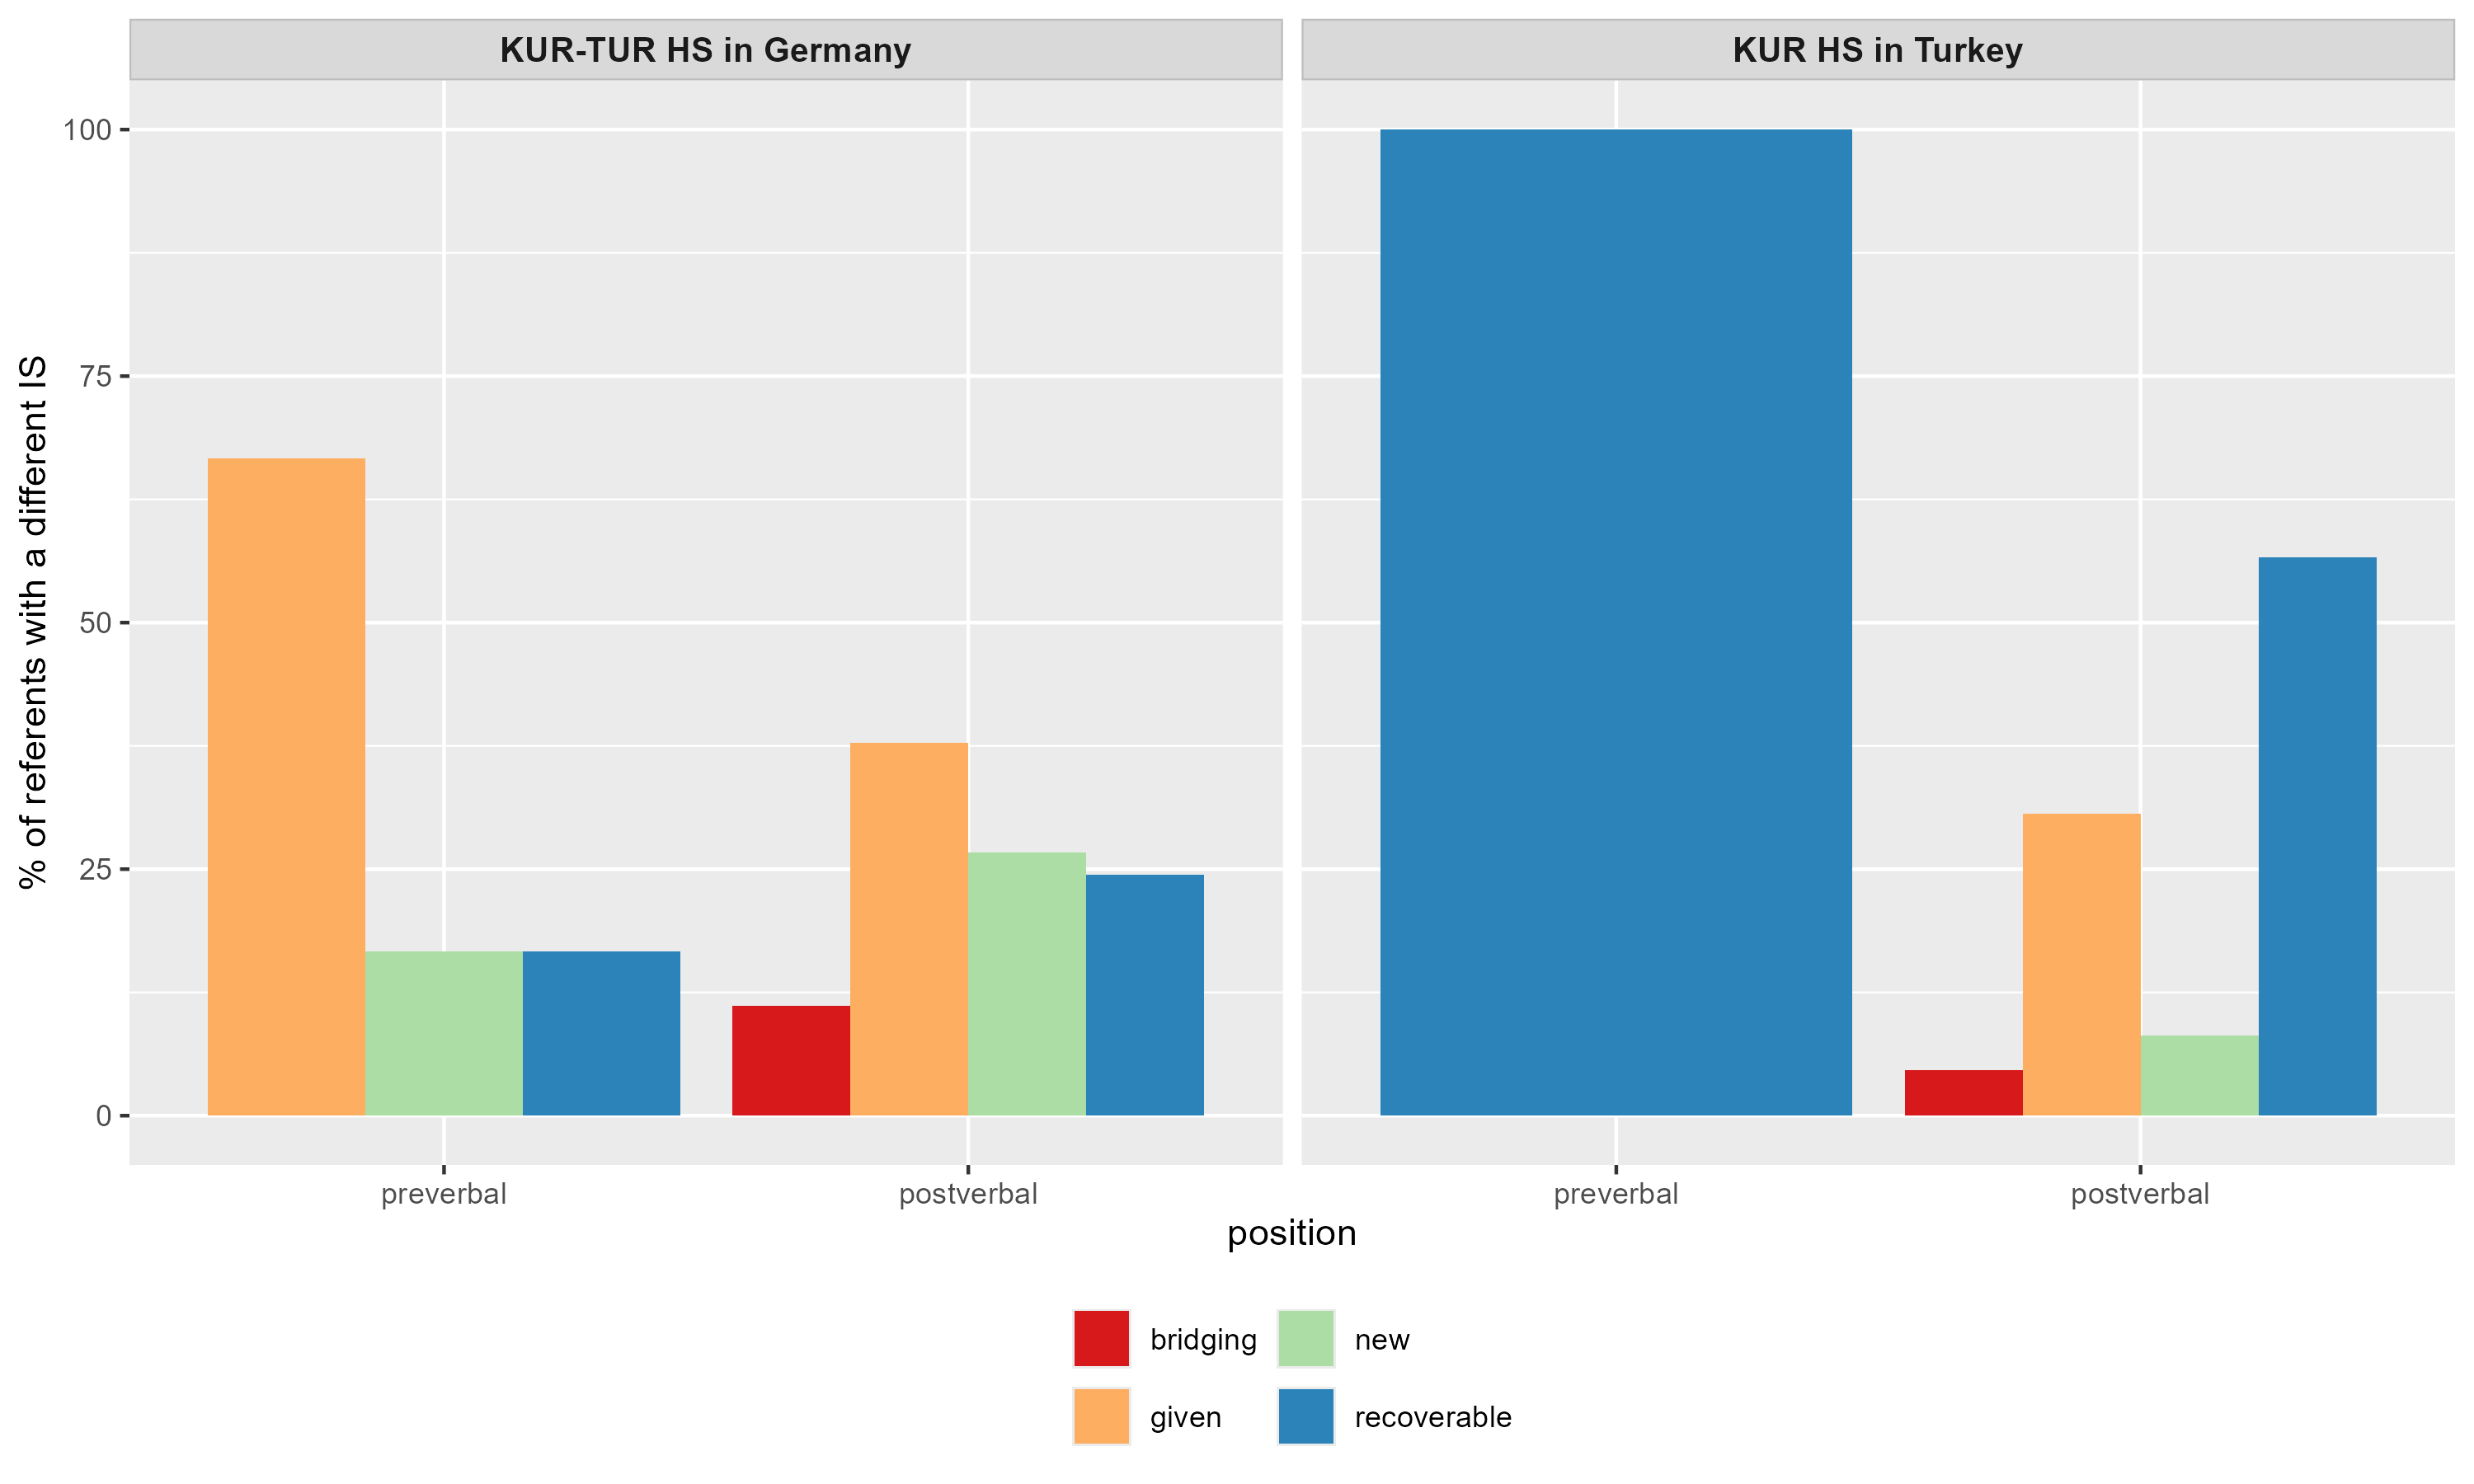
\includegraphics[width=\textwidth]{figures/iefremenko-img018.png}
\caption{\label{fig:key:19}Frequency distribution of goal arguments flagged with case or a locational noun according to their information status.}
\end{figure}

\figref{fig:key:19} illustrates the frequency distribution of goal arguments based on their information status, calculated relative to the total number of goal arguments within each speaker group. For noncanonically placed goal arguments flagged with case or a locational noun (i.e., those in the pre-predicate position), all preverbal goals in Turkey are classified as recoverable information (100\%). In contrast, speakers in Germany place 66.67\% of preverbal goals as given, 16.67\% as new, and 16.67\% as recoverable, although the overall number of preverbal goals is low. Regarding post-predicate goals, speakers in Turkey primarily place recoverable goals (56.65\%) and given goals (30.64\%), with smaller proportions of new (8.09\%) and bridging (4.62\%) referents. In Germany, post-predicate goals include given (37.78\%), new (26.67\%), recoverable (24.44\%), and bridging (11.11\%) referents. Taken together, these percentages indicate that information status does not systematically influence whether goals are placed pre- or post-predicatively in either group, as all types of referents can appear in both positions.

Consequently, these findings do not align with those of \citet{Asadpour2021}, and several factors may contribute to this discrepancy. First, as previously mentioned, Asadour's findings are based on a different variety of Kurdish. Additionally, the current data may not be fully suitable for analyzing information status, given that each participant narrated the same story four times in each language, with a 10-15-minute break between formal and informal sessions and a gap of three to seven days between language sessions.

\subsection{Exploring possible factors influencing the position of adpositional goals (excluding locational nouns) in Kurmanji}\label{sec:key:6.3.3}

The following three analyses will focus on adpositional goals, specifically basic prepositions—either alone or in combination with a locational noun—as well as circumpositions and postpositions, while excluding locational nouns. In the dataset, the position of these adpositional goals varies, and the previous research states that the position of adpositional goals is indeed flexible (\citealt{Haig2014, Haig2018}). Thus, this section will examine which variables may influence the placement of adpositional goals of motion in either the pre- or post-predicate position. Similar to the analysis of goals flagged with case or locational nouns, the first step will be to investigate potential differences in the placement of adpositional goals between the groups. Furthermore, the effects of formality and mode on the positioning of adpositional goals will be analyzed, followed by an exploration of the influence of the information status of these goals.

Importantly, previous research has also shown that the placement of adpositional goals differs among various dialects of Kurmanji (\citealt{Haig2014, Haig2018, Gundogdu2019}). However, because the data were collected in Ankara without accounting for dialectical differences, this factor remains unaddressed in the study.

\subsubsection{The effect of the speaker group on the placement of adpositional goals (excluding locational nouns) in Kurmanji.}\label{6.3.3.1}

The findings in \sectref{sec:key:6.3} indicate that adpositional goals can be found in both pre- and post-predicate positions, and their placement does not appear to be influenced by the speaker group or the majority language of the speakers. To statistically verify whether the speaker group affects the use of case-flagged goals in the pre-predicate position, a generalized logistic mixed-effects model was used, following a binomial distribution. In this model, Position (with preverbal coded as 1 and postverbal coded as 0) served as the dependent variable, while Group (comprising Kurmanji speakers in Turkey (Tubi) and Kurmanji speakers in Germany (Debi)) was treated as a fixed effect. Participant was included as a random variable. The results of the regression analysis are summarized in \tabref{tab:key:15}.


\begin{table}\small
\begin{tabularx}{\textwidth}{XYY}
\lsptoprule
\textbf{Random effects:} & & \\
\midrule
\textbf{Groups} & \textbf{Variance} & \textbf{Standard} \textbf{Deviation}\\
Participant (Intercept) & 2.29 & 1.51\\
% \lspbottomrule
\midrule
\end{tabularx}

\begin{tabularx}{\textwidth}{Xrrrr}
% \lsptoprule
\textbf{Fixed effects:} & & & & \\
\midrule
\textbf{Fixed} \textbf{effect} & \textbf{Estimate} & \textbf{Std. Error} & \textbf{z-value}  & \textbf{\textit{p}-value}\\
Intercept & -0.90 & 0.97 & -0.94 & .35\\
Group (Tubi) & 0.97 & 1.08 & 0.90 & .37\\
\lspbottomrule
\end{tabularx}
\caption{\label{tab:key:15}Regression table for glmer with the dependent variable Position and the independent variable Group.}
\end{table}

As anticipated, the results of the regression analysis indicate that the speaker group has no significant effect on goal position.

\subsubsection{The effect of formality and mode on the placement of adpositional goals (excluding locational nouns) in Kurmanji.}\label{sec:key:6.3.3.2}

To determine whether formality and mode influence the position of adpositional goals, a binomial generalized linear mixed-effects model was used to assess the effects of these factors on the placement of adpositional goals. In this model, the dependent variable is the Position of Adpositional Goals (preverbal coded as 0 and postverbal coded as 1), while the independent variables include the interaction between Formality (formal vs. informal) and Mode (spoken vs. written). The model also accounted for individual variation within the data by incuding the variable Participant as a random variable. An overview of the regression results can be found in \tabref{tab:key:16}.

\begin{table}\small
\begin{tabularx}{\textwidth}{XYY}
\lsptoprule
\textbf{Random effects:} & & \\
\midrule
\textbf{Groups} & \textbf{Variance} & \textbf{Standard} \textbf{Deviation}\\
Participant (Intercept) & 3.07 & 1.75\\
% \lspbottomrule
\midrule
\end{tabularx}

\begin{tabularx}{\textwidth}{Xrrrr}
% \lsptoprule
\textbf{Fixed effects:} & & & & \\
\midrule
\textbf{Fixed} \textbf{effect} & \textbf{Estimate} & \textbf{Std. Error} & \textbf{z-value}  & \textbf{\textit{p}-value}\\
Intercept & {}-0.87 & 0.60 & {}-1.44 & .14\\
Formality (informal) & 1.26 & 0.62 & 2.02 & $.43^{*}$\\
Mode (written) & 0.53 & 0.63 & 0.85 & .39\\
\lspbottomrule
\end{tabularx}
\caption{\label{tab:key:16}Regression table for binomial glmer with the dependent variable Position of ADP Flagged Goals and the independent variables Formality and Mode.}
\end{table}

\newpage
Formality: Formality is a binary independent variable assigned the levels formal and informal in my study. As seen in \tabref{tab:key:16}, informality significantly facilitates the placement of adpositional goals of motion in the post-predicate position. This is also demonstrated in \figref{fig:key:20}.

Mode: Mode is a binary independent variable with the levels spoken and written. The model shows no reliable or significant effect of Mode.

\begin{figure}[t]
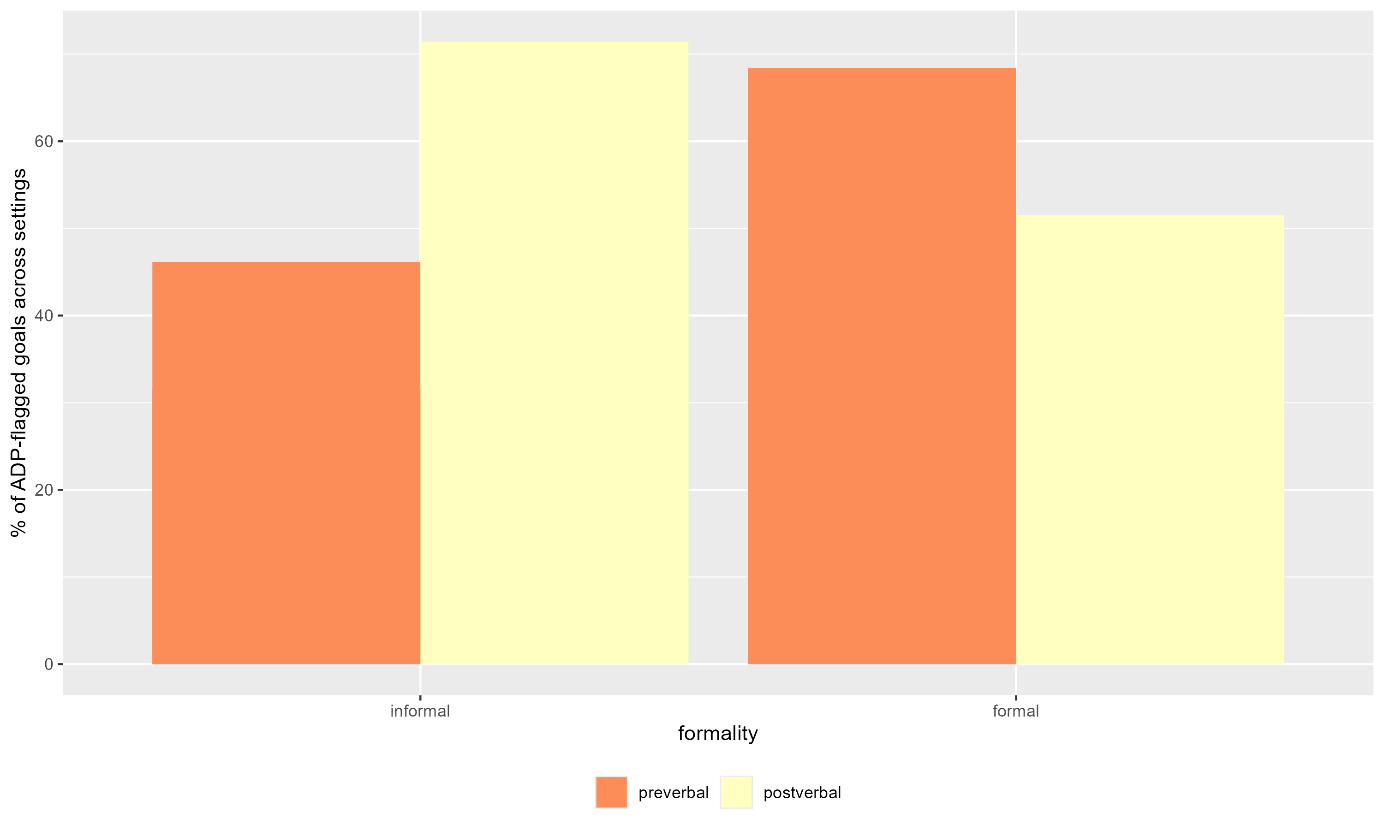
\includegraphics[width=\textwidth]{figures/iefremenko-img019.png}
\caption{\label{fig:key:20}Frequency distribution of ADP-flagged goals of motion in the pre- and post-predicate position across formal and informal settings.}
\end{figure}

Thus, the regression analysis showed the effect of formality: while the post-predicate goals are more likely to occur in the informal data, the pre-predicate goals were more likely to be used in the formal communicative situations.

\subsubsection{The effect of information structure on the placement of adpositional goals (excluding locational nouns)}\label{sec:key:6.3.3.3}

Next, the role of information structure in the placement of adpositional goals will be explored. Similar to the analysis of goals of motion flagged with case or a locational noun, the information status of the adpositional goal arguments has been annotated, differentiating between new, given, bridging, and recoverable statuses. The results of this analysis are presented in \figref{fig:key:21}.

\begin{figure}
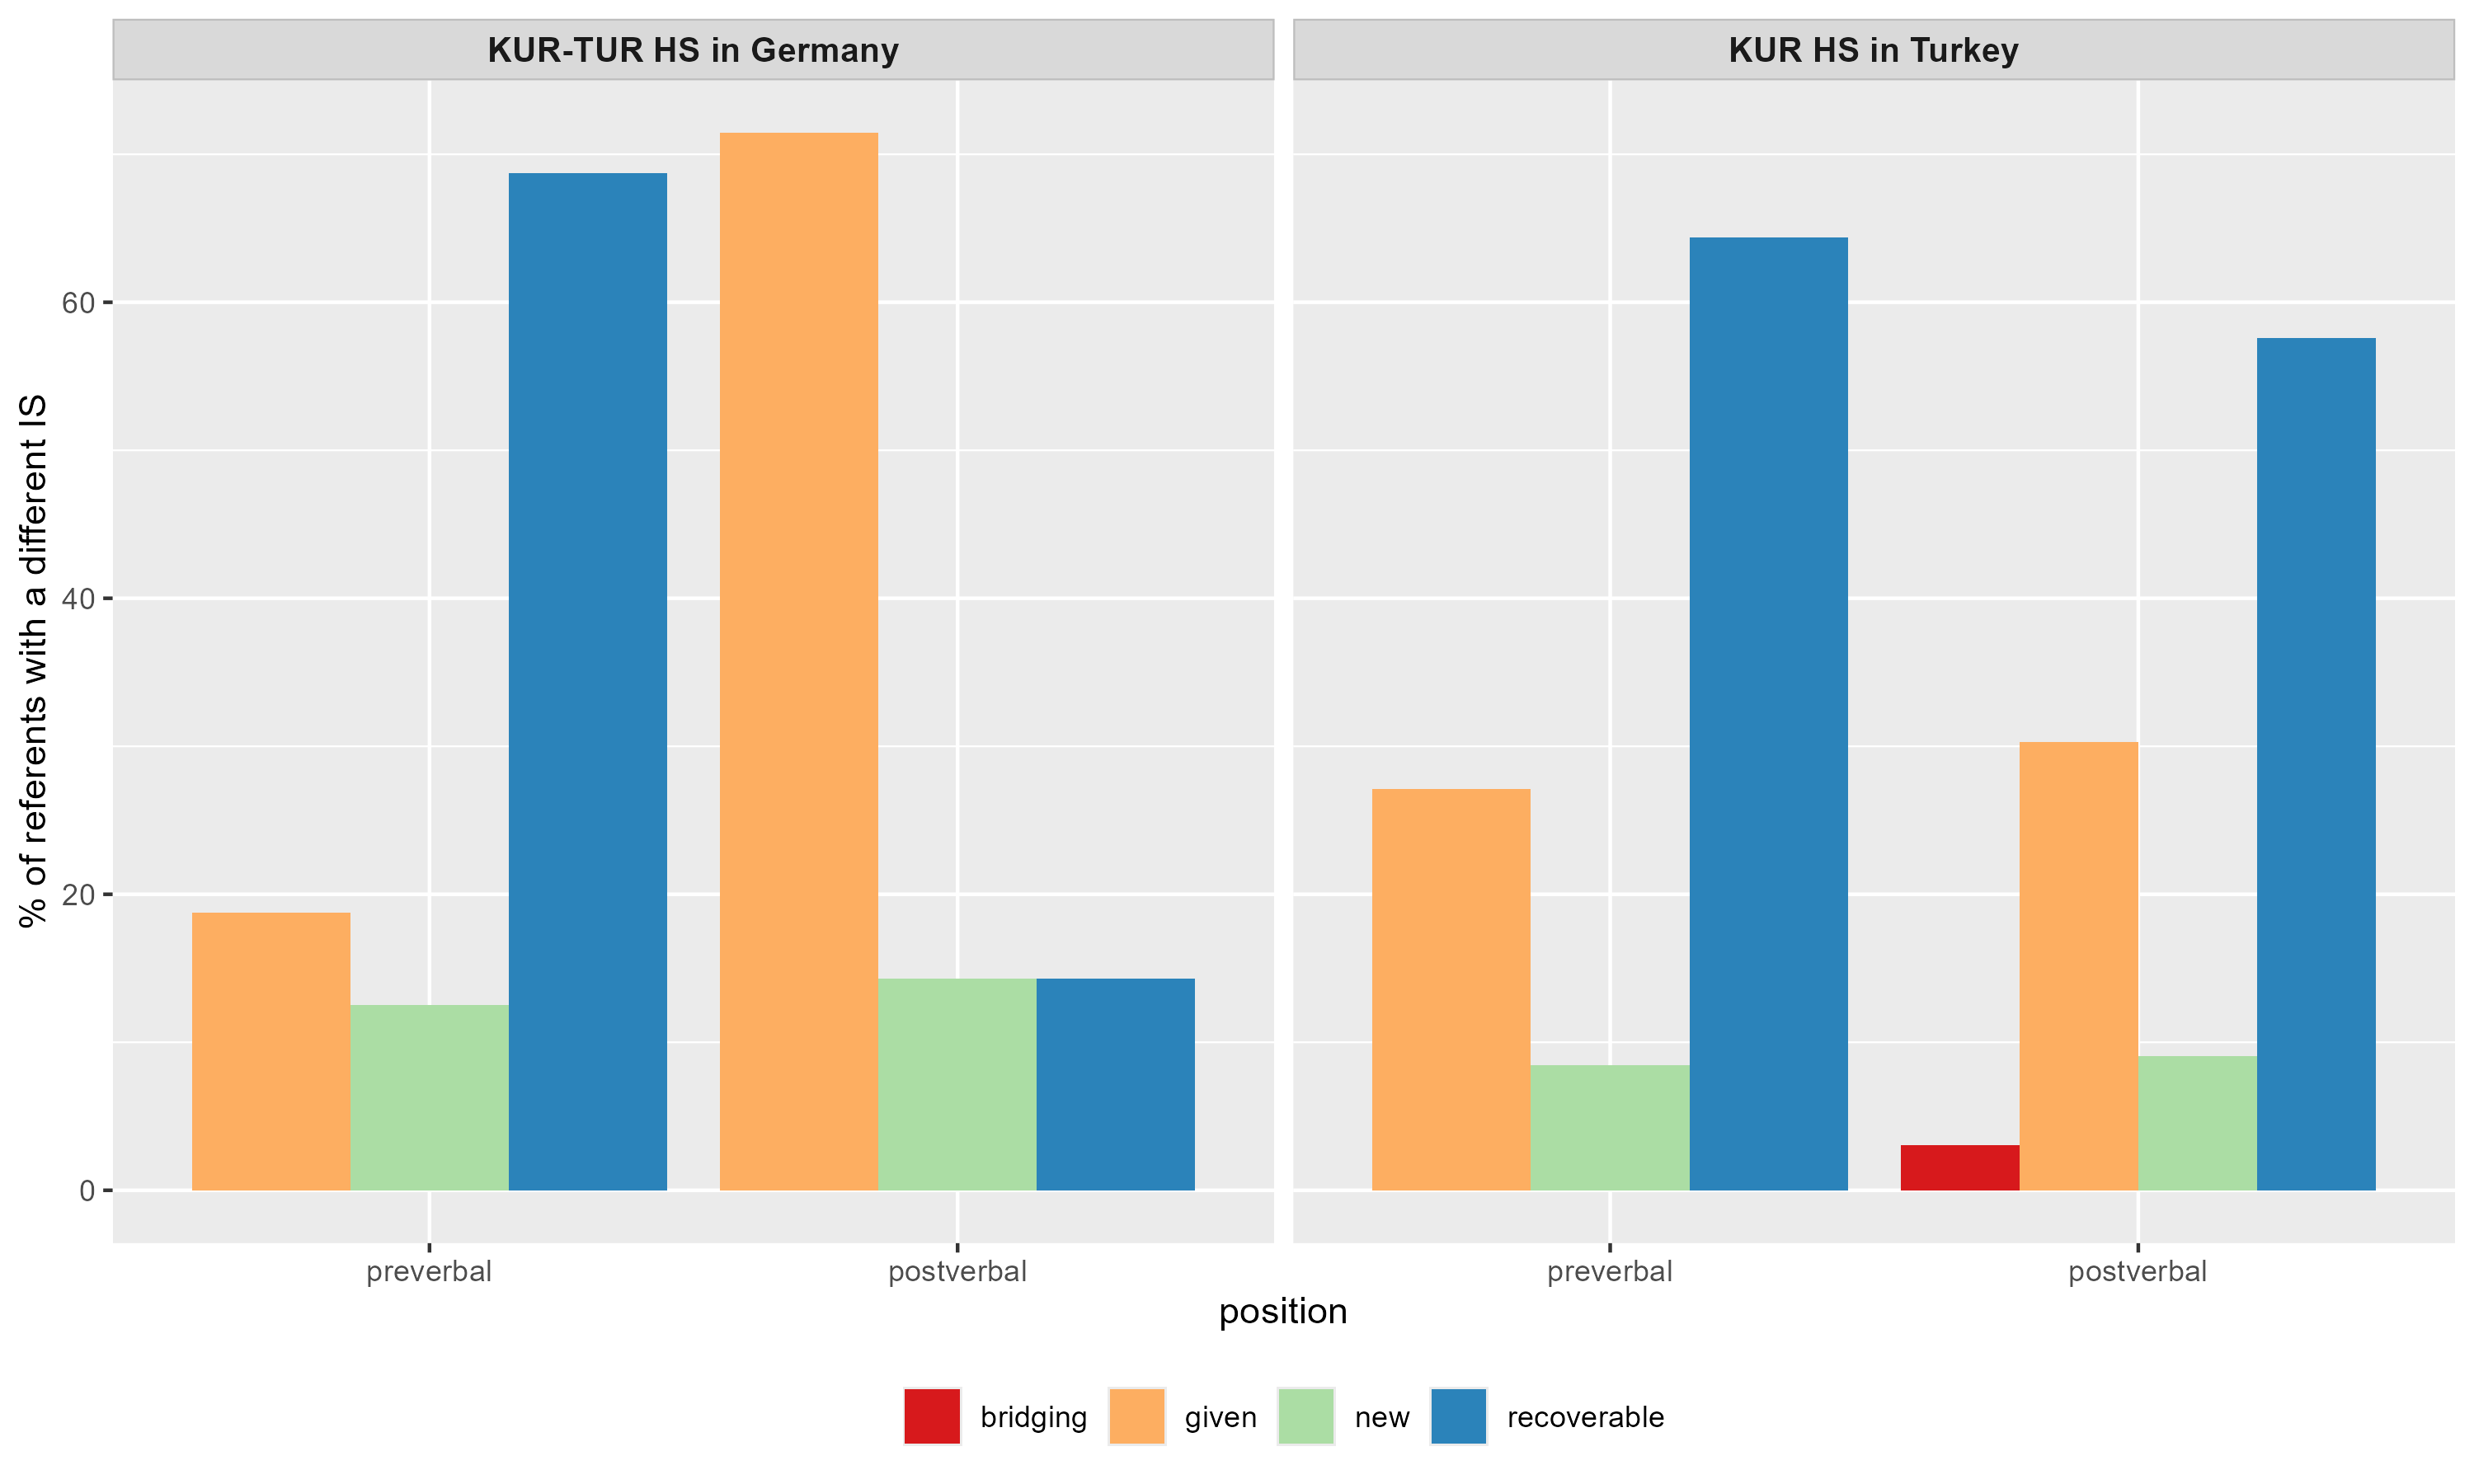
\includegraphics[width=\textwidth]{figures/iefremenko-img020.png}
\caption{\label{fig:key:21} Frequency distribution of goal arguments flagged with an adposition according to their information status.}
\end{figure}

\figref{fig:key:21} illustrates that recoverable and given goals are the most frequent in the dataset, although their placement varies by speaker group. In Turkey, postverbal goals are most often recoverable (57.6\%), followed by given (30.3\%) and new referents (9.1\%), while bridging referents are virtually absent (3.0\%). In the preverbal position, recoverable referents are again the most frequent (64.4\%), with given (27.1\%) and new (8.5\%) referents occurring less often. This indicates a relatively balanced distribution across positions, with recoverable information dominating in both. In Germany, postverbal goals are predominantly given (71.4\%), with recoverable and new referents occurring much less frequently (14.3\% each). In contrast, preverbal goals are mostly recoverable (68.8\%), followed by given (18.8\%) and new (12.5\%) referents. Hence, there is no clear effect of information status on the placement of adpositional goals of motion.

\subsection{Interim summary}\label{sec:key:6.3.4}

To summarize the findings on goals of motion in Kurmanji, results indicate that goals of motion flagged with case or an adposition can appear in both pre- and post-predicate positions, though the post-predicate position is generally preferred. Previous research (\citealt{Haig2014, Gundogdu2019}) suggests that goals of motion flagged with case or a locational noun are restricted to the post-predicate position. However, the data analyzed here include instances where such goals also appear in the pre-predicate position.

Regression analyses revealed no correlation between group, formality and mode, and the placement of case-flagged goals or those marked with locational nouns. Besides, information structure does not seem to play a role of the position of these constituents. However, qualitative analysis showed that in the Kurmanji data from Turkey, all pre-predicate occurrences of case-flagged goals appear in the same construction \textit{erdê ketin} (‘to fall on the ground’), whereas the data from Germany exhibit greater variation in verb usage with case-flagged arguments in the pre-predicate position. Similarly, in the data from Turkey, locational nouns in the pre-predicate position predominantly occur in the construction \textit{hemberî rê} (‘across the road’), while no such pattern emerges in the data from Germany.

Regarding goals flagged with adpositions, previous research (\citealt{Haig2014, Gundogdu2019}) suggests that their position is more flexible compared to goals of motion flagged with case or locational nouns. The present findings confirm this variability. Notably, regression analysis identified formality as a significant predictor for the placement of adpositional goals: while the post-predicate position is more frequent in the informal situations, the pre-predicate position is preferred in the formal settings.

\subsection{Addressees of verbs of speech}\label{sec:key:6.3.5}

The focus now shifts to the second most frequent type of goals in the data: addressees of verbs of speech. Similar to goals of motion in Kurmanji, addressees of verbs of speech can be flagged with the oblique case (see example \ref{ex:key:77} or an adposition (see example \ref{ex:key:78}).


\ea \label{ex:key:77} Kurmanji, TUbi10MK\_fwK \\
\gll Ez    di-xwaz-im   agahî     bi-di-m     we \\
\textsc{1sg.nom}  \textsc{prs-}want-\textsc{1sg}  news    \textsc{subj-}give-\textsc{1sg}    you.\textsc{2pl}\\
\glt ‘I want to inform you.’ 
\z

\ea%76
  \label{ex:key:78} Kurmanji, TUbi05MK\_fwK \\
\gll Mi     go     e  ji   te     ra   bi-bêj-im \\
\textsc{1sg.obl}    say\textsc{.pst}    hm  to  \textsc{2sg.obl}    \textsc{circ}  \textsc{subj}-say-\textsc{1sg}  \\
\glt ‘I said, I am telling to you.’  
  \z

As with goals of motion, the position of addressee arguments depends on the type of flagging and the dialect. According to \citet{Gundogdu2019}, case-flagged goals always appear post-predicate (as in example \ref{ex:key:77}), while adpositional addressees are typically placed in the pre-predicate position (as in example \ref{ex:key:78}). However, regional variation influences both the position and the types of adpositions used in Kurmanji (\citealt{Haig2014}, \citealt{Haig2022}). In southeastern dialects, addressees are case-flagged and post-predicate, whereas in northern dialects, they are primarily adpositional and appear pre-predicatively. Additionally, different northern dialects exhibit distinct preferences for adpositional flagging: in the Northern dialect (e.g., Muş), speakers predominantly use the circumposition \textit{ji…ra} (‘to’), while in the Northwestern dialect (e.g., Malatya), the postposition \textit{…ra} (‘to’) is preferred (\citealt{Gundogdu2019}). Notably, addressees flagged with a circumposition cannot be placed post-predicatively and must always appear in the pre-predicate position (\citealt{Gundogdu2019}).

The frequency distribution of addressees flagged with the oblique case or an adposition in either the pre- or post-predicate position is presented in \figref{fig:key:22}.

\begin{figure}
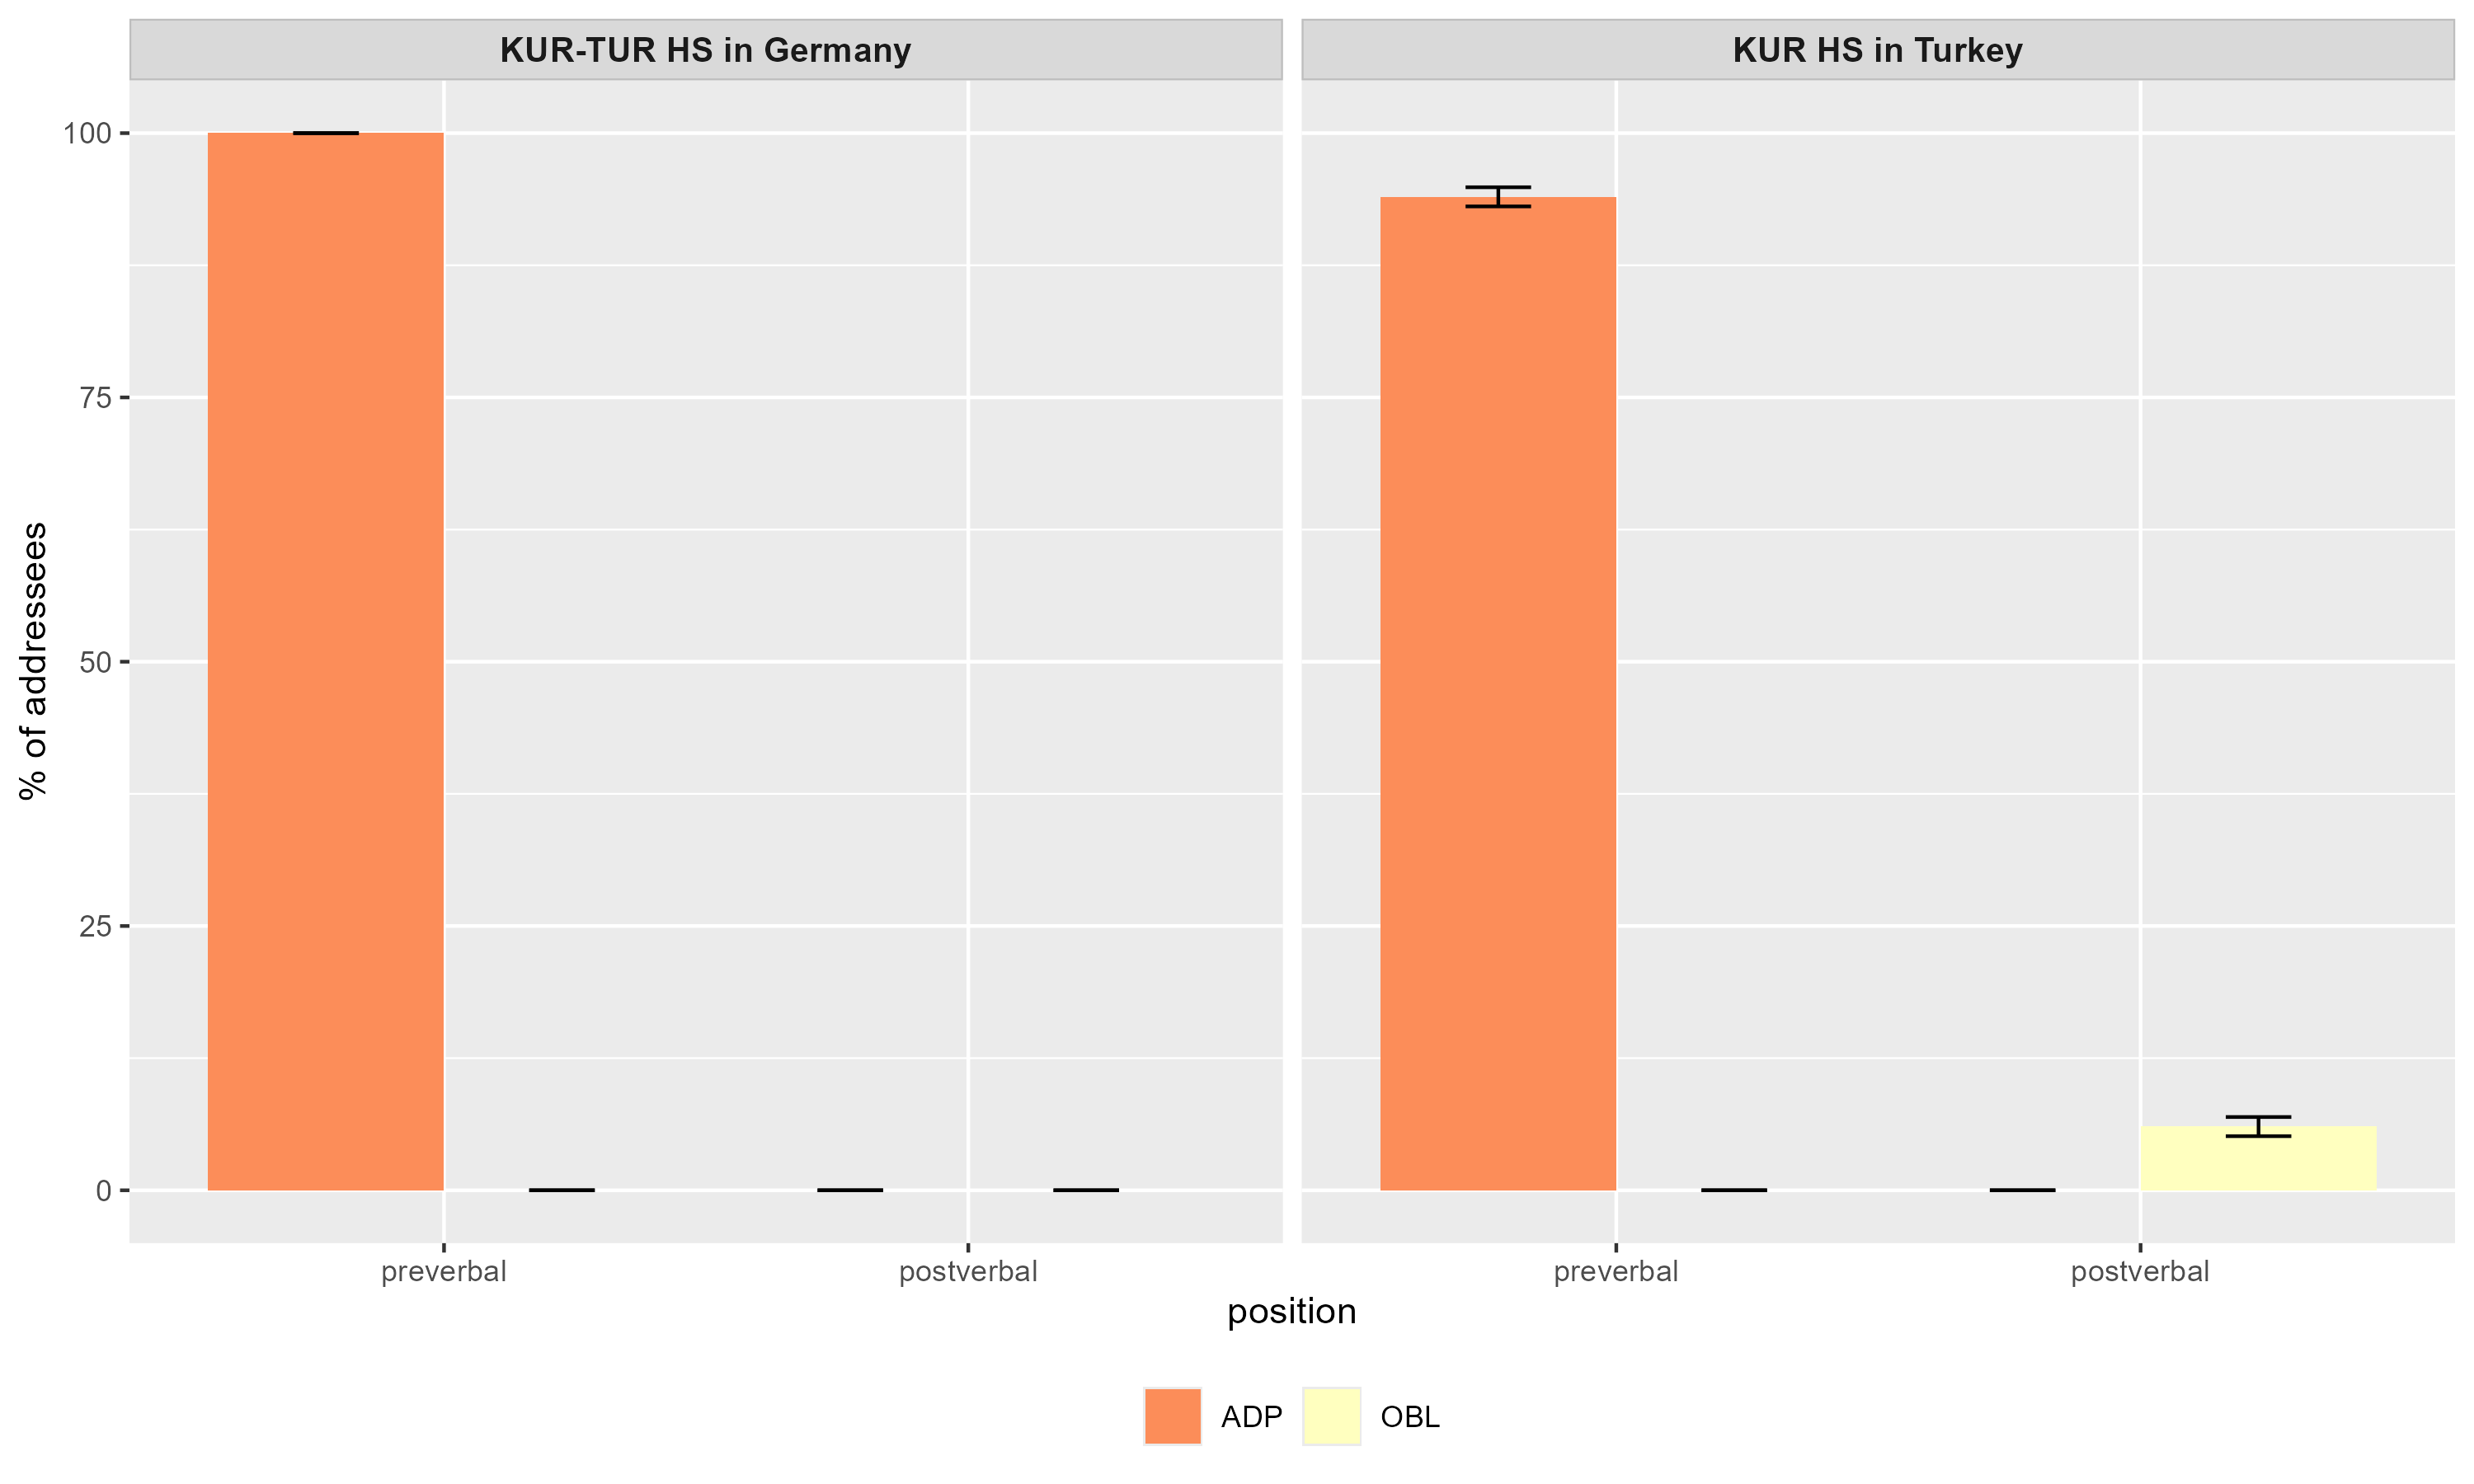
\includegraphics[width=\textwidth]{figures/iefremenko-img021.png}
\caption{\label{fig:key:22}Frequency distribution of addressees flagged with the oblique case or an adposition in the pre- and post-predicate position (in \%) in relation to the total number of addressees.}
\end{figure}

As mentioned in \sectref{sec:key:6.3}, the video shown to the participants elicited fewer addressees compared to goals of motion. The data includes 24 instances of arguments of verbs of speech from Kurmanji speakers in Turkey and only three instances from Kurmanji speakers in Germany. Therefore, the frequencies in the plot should be interpreted with caution.

The left-hand plot in \figref{fig:key:22} illustrates that all three examples from Kurmanji-Turkish HS in Germany are flagged with an adposition and appear in the pre-predicate position. Similarly, the right-hand plot shows that speakers in Turkey also predominantly flag addressees with an adposition and place them preverbally, aligning with previous research (\citealt{Gundogdu2019, Haig2022}).

\tabref{tab:key:17} presents the absolute number of addressees flagged with either case or an adposition in the pre- or post-predicate position. Additionally, the table provides information on the type of adposition used, distinguishing between the circumposition \textit{ji…ra} and the postposition \textit{…re/ra}.

\begin{table}
\begin{tabularx}{\textwidth}{llYYY}
\lsptoprule
Country & Position & OBL flagged & Flagged with circumposition
(\textit{ji…re/ra}) & Flagged with a postposition (\textit{re/ra})\\
\midrule
Turkey & pre- & - & 16 & 5\\
& post- & 3 & - & -\\
Germany & pre- & - & 1 & 2\\
& post- & - & - & -\\
\lspbottomrule
\end{tabularx}
\caption{\label{tab:key:17} The absolute number of addressees flagged with the help of oblique case or an adposition placed in the pre- or post-predicate position.}
\end{table}

\tabref{tab:key:17} indicates that speakers in Turkey predominantly flag addressees with the circumposition \textit{ji…ra} and place them in the pre-predicate position. However, in both country groups, some addressees are flagged using the postposition \textit{re/ra}—five instances in the data from Turkey and two from Germany—all of which occur in the pre-predicate position.

In addition to addressees marked with a circumposition or postposition, three instances of case-flagged addressees appear in the data. As previously mentioned, the only canonical position for case-flagged goals is post-predicate. Consistently, all three examples in the data follow this pattern (see example 79).

\ea \label{ex:key:79} Kurmanji, TUbi11FK\_iwK \\
\gll cane pesiye   di-xwaz-im     silav-ek   bi-di-m     te  \\
dear  {}  \textsc{prs-}want-\textsc{1sg}    hello-\textsc{indf}  \textsc{subj-}give-\textsc{1sg}    you.\textsc{2pl} \\
\glt ‘My dear, I would like to say hello to you’. 
\z

Due to the limited number of addressees in the data, it is not possible to run statistical models to examine correlations between variables such as speaker group, formality, mode, or information status and the position of addressees.

However, the quantitative analysis indicates that Kurmanji speakers in both Turkey and Germany follow the word order patterns observed in previous studies. Case-flagged goals consistently appear in the immediate post-predicate position, while adpositional goals are placed pre-predicatively. These findings confirm that the position of addressees is primarily determined by the type of flagging.

Regarding the effect of formality and mode, the qualitative analysis of the data revealed that addressees appear in both pre- and post-predicate positions across all communicative situations. This suggests that formality and mode do not influence the positioning of addressees. Additionally, all addressees in the data are expressed using second-person singular and plural pronouns in contexts such as "I’d like to tell you about...," which precludes an analysis of information status for addressees.

\subsection{Non-goal constituents in the post-predicate position}\label{sec:key:6.3.6}

As previously demonstrated, Kurmanji is an OVX language, with X reserved for goal of motion, addressees of verbs of speech and recipients of verbs of transfer. However, as illustrated earlier in this chapter and shown again in \figref{fig:key:23} for convenience, there are also other constituents in the data placed in the post-predicate position.

\begin{figure}
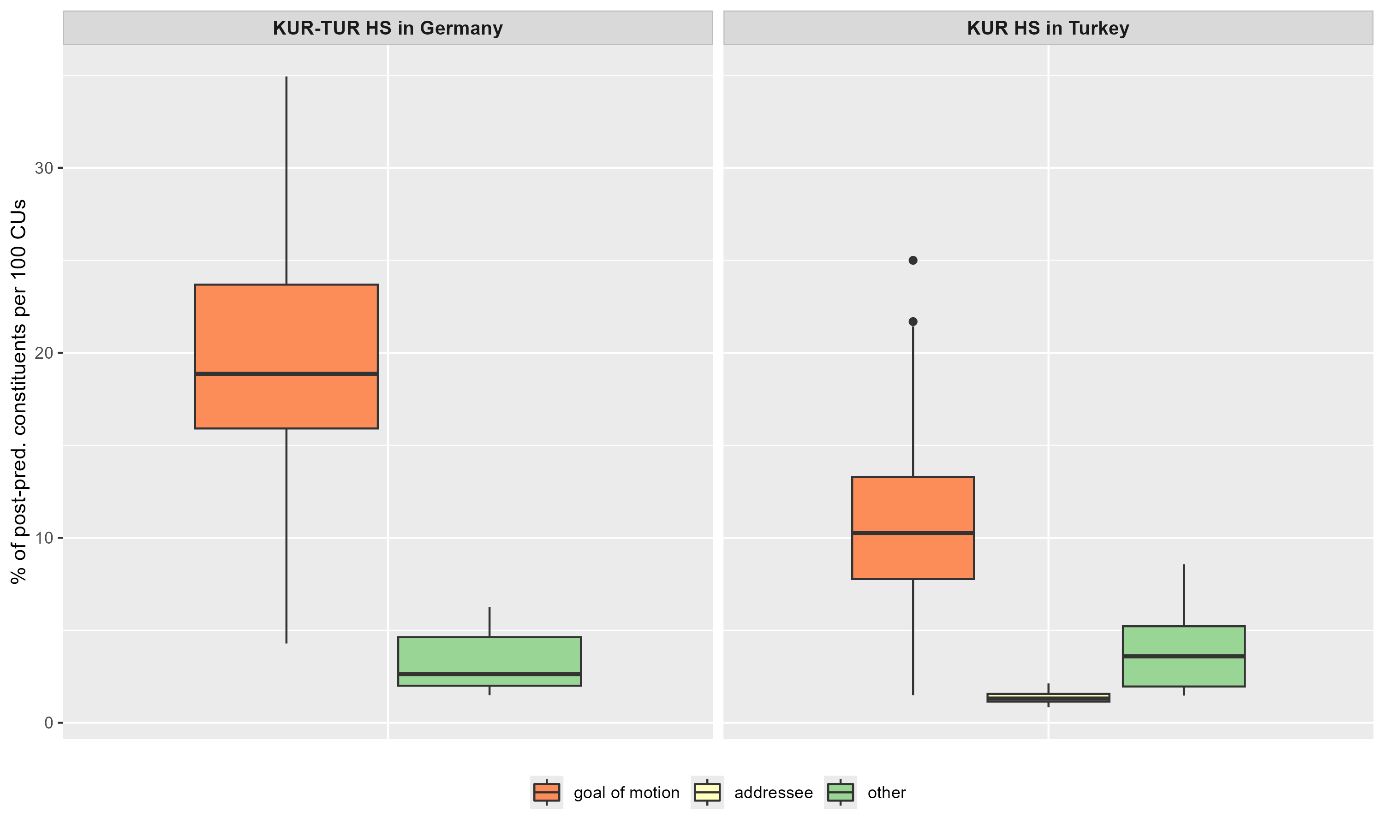
\includegraphics[width=\textwidth]{figures/iefremenko-img015.png}
\caption{\label{fig:key:23}Types of post-predicate structures in Kurmanji in two country groups.}
\end{figure}

\figref{fig:key:23} illustrates that approximately 3\% (n=15) of all the CUs in the data from Germany and about 4\% (n=55) of the CUs in the data from Turkey contain non-goal constituents in the post-predicate position. To determine whether one group shows a statistically significant tendency to place non-goal constituents in the post-predicate position compared to the other, a linear regression model was conducted, with the Percentage of Non-Goal Constituents in the Post-Predicate Position as the dependent variable and Group as the fixed effect.

\begin{table}
\begin{tabularx}{\textwidth}{XYYYY}
\lsptoprule
\textbf{Fixed effect} & \textbf{Estimate} & \textbf{Std. Error} & \textbf{t-value}  & \textbf{p-value}\\
\midrule
(Intercept) & 3.29 & 0.74 & 4.40 & $.0001^{***}$\\
Group (Tubi) & 0.71 & 0.86 & 0.82 & .41 \\
\lspbottomrule
\end{tabularx}
\caption{\label{tab:key:18}Regression table for LM with a dependent variable Percentage of Non-Goal Constituents in the Post-Predicate Position and an independent variable Country.}
\end{table}

\largerpage
Group: The variable Group is treated as a binary variable with two levels: Germany and Turkey. The model did not reveal any significant effects related to the country variable.

The linear model indicated that there are no significant differences between the groups regarding the placement of non-goal constituents in the post-predicate position. Therefore, the observed higher frequency of post-predicate structures in Germany, as discussed in \sectref{sec:key:6.1}, cannot be attributed to a greater number of non-goal constituents used by speakers in Germany compared to those in Turkey.

To further explore the characteristics of non-goal constituents placed in the post-predicate position in Kurmanji and to understand the source of the occurrence of such structures, the following analysis will examine various features, including phonological weight, types of constituents, and their semantic roles.

\subsubsection{Weight of non-goal post-predicate constituents in Kurmanji}\label{sec:key:6.3.6.1}

The analysis will begin with the weight of non-goal constituents in the post-predicate position. It is anticipated that speakers will preferentially place longer segments in this position, as this strategy may help mitigate the limitations in working memory capacity experienced by both speakers and listeners.

Following \citep{Haignforth}, four types of weight for non-goal post-predicate constituents will be identified, paralleling the analysis of post-predicate constituents in Turkish described in Section \ref{sec:key:5.3.1}. Post-positive constituents are italicized for clarity.

\begin{itemize}
\item Weight 1: a single phonological word.

\ea
  \label{ex:key:80} Kurmanji, TUbi15MK\_isK \\
     \gll Ez     ji   wir   çû-m     \textit{yanî}\\
\textsc{1sg.nom}  from  there  go\textsc{.pst-1sg}  well\\
\glt ‘I was going from there yani.’
  \z


\item{Weight 2:} two phonological words.

\ea%79
  \label{ex:key:81} Kurmanji, TUbi30FK\_isK \\
     \gll û:   kûçik   jî   tirsîya     \textit{ji}   \textit{top-ê} \\
and  dog  also  scare\textsc{.pst.3sg}  from  ball-\textsc{obl}  \\
\glt ‘And the dog got scared of the ball.’ 
  \z


\item{Weight 3:} three phonological words.

\ea%80
  \label{ex:key:82} Kurmanji, TUbi26MK\_isK \\
     \gll Mêr   û   jin-ek-î     ji   wê   da   di-hat-in \textit{tevî}     \textit{sebî-yê}     \textit{xwe}\\
man  and  woman-\textsc{indf-obl.f}  from  her  \textsc{post}  \textsc{prs}-come-\textsc{3pl} together  baby-\textsc{ez}  \textsc{refl}\\
\glt ‘A man and a woman were coming from her with their child.’  
  \z


\item{Weight 4:} four or more phonological words.

\ea%81
  \label{ex:key:83} Kurmanji, DEtr10FK\_iwK \\
     \gll Çink-ek   hawo     \textit{ba}   \textit{guddik}, \textit{ba}   \textit{torb-ok}  \textit{sew}\\
woman\textsc{-indf}  have\textsc{.pst.3sg}  with  dog   with  bag-\textsc{indf}  apple\\
\glt ‘There was a woman with a dog, with a bag of apples.’ 
  \z

\end{itemize}

Thus, in essence, every element can contribute to the overall weight of a constituent. Notably, unlike Turkish, Kurmanji frequently uses adpositions that add additional weight to post-predicate structures. However, adpositions comprising two or three elements, such as circumpositions, are considered as constituents with a weight of 1. For example, in \REF{ex:key:82}, the post-predicate structure \textit{di bûyerê de} (‘in the incident’) is assigned a weight of two phonological words, as the circumposition \textit{di…de} is treated as a single element in this analysis.

\ea%82
  \label{ex:key:84} Kurmanji, TUbi17FK\_fsK \\
        \gll Lê   kesek     birîndar   ne-bû     di   buyer-ê   de\\
but  somebody  injured    \textsc{neg}-be\textsc{.pst.3sg} \textsc{circ}  accident-\textsc{obl.f} \textsc{circ}\\
\glt ‘But no one was injured in the incident.’ 
  \z

The results of the analysis of the weight of non-goal post-predicate structures in Kurmanji are presented in \figref{fig:key:24}.

\begin{figure}[b]
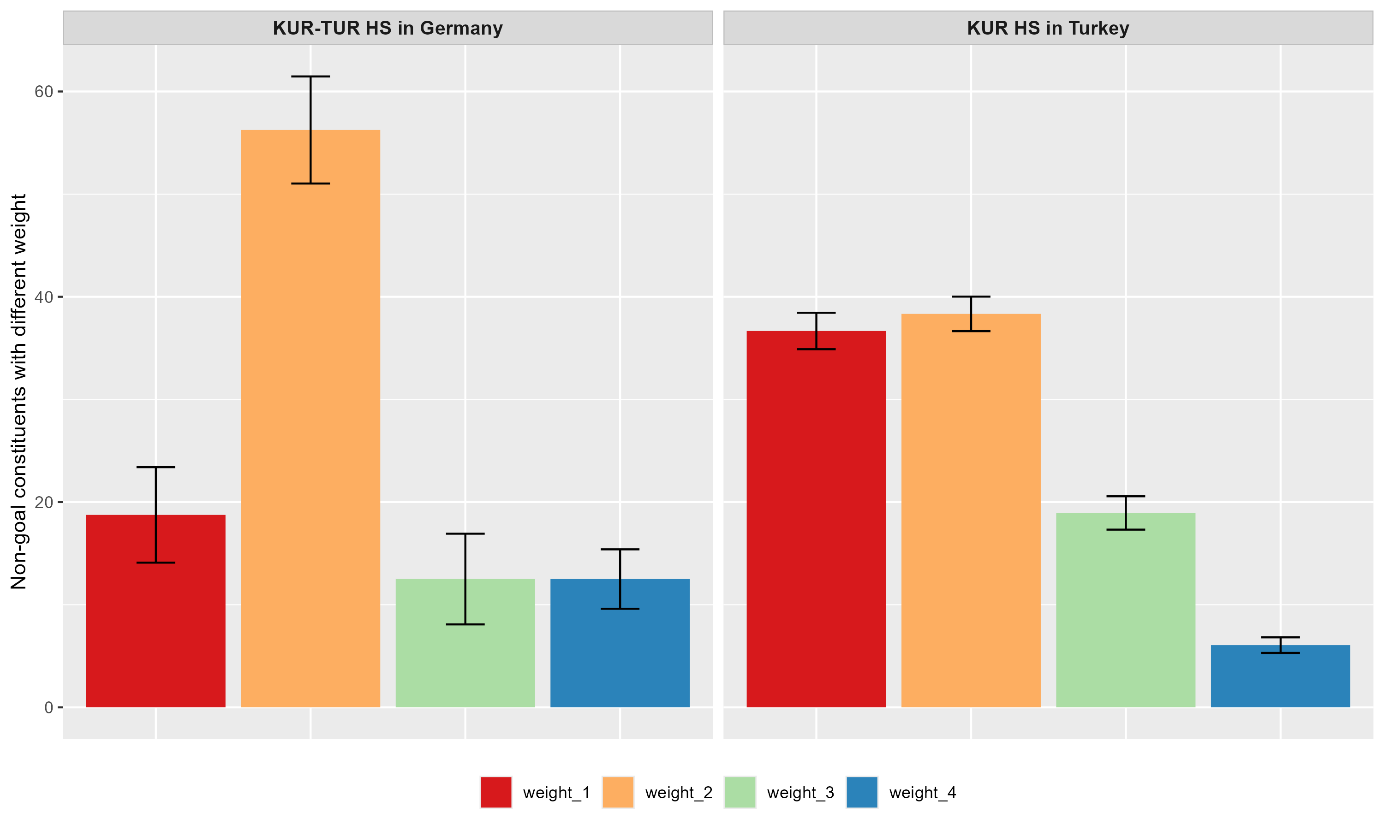
\includegraphics[width=\textwidth]{figures/iefremenko-img022.png}
\caption{\label{fig:key:24}Frequency distribution of non-goal post-predicate structures with different weight calculated in relation to the total number of non-goal post-predicate structures in each group.}
\end{figure}

\figref{fig:key:24} illustrates the frequency distribution of non-goal post-predicate structures with varying weights, calculated in relation to the total number of non-goal post-predicate structures within each speaker group. Error bars represent the standard error. The analysis reveals that speakers in Germany predominantly use post-predicate structures consisting of two elements, whereas speakers in Turkey exhibit a roughly even distribution of examples between post-predicate structures composed of one and two phonological words.

It is important to note, however, that the frequency distribution depicted in \figref{fig:key:24} is based on a very limited number of examples, particularly within the German group. Consequently, no statistical tests will be conducted for this or the subsequent analyses of non-goal constituents.

\subsubsection{Types of non-goal post-predicate structures in Kurmanji}\label{sec:key:6.3.6.2}

The following section will focus on the types of non-goal constituents previously discussed. The categorization of these types is based on the classification used for post-predicate structures in Turkish (see \sectref{sec:key:5.3.2}), as outlined by \citet{SchroederEtAl2024}. Accordingly, three types of constituents will be identified:

\begin{itemize}
\item Type 1: nominal constituents


\ea \label{ex:key:85} Kurmanji, TUbi17FK\_fsK \\
\gll Lê   kesek     birîndar   ne-bû       \textit{di}   \textit{buyer-ê}   \textit{de}\\
but  somebody  injured    \textsc{neg}-be\textsc{.pst.3sg}  in  accident-\textsc{obl}  \textsc{circ}\\
\glt ‘But no one was injured in the incident.’ 
  \z


\item Type 2: adverbs


\ea\label{ex:key:86} Kurmanji, TUbi18MK\_fsK \\
\gll Arabay fîren   kir     \textit{niha}\\
car  break  do\textsc{.pst.3sg}  now\\
\glt ‘The car braked now.’ 
  \z


\item Type 3: discourse markers


\ea \label{ex:key:87} Kurmanji, TUbi15MK\_isK \\
\gll Ez   ji   wir   çû-m     \textit{yanî}\\
I  from  there  go\textsc{.pst-1sg}  well\\
\glt ‘I was going from there yani’ 
  \z

\end{itemize}

If a post-predicate structure included two or more types, each type was calculated separately. The analysis of the different types of non-goal constituents is presented in \figref{fig:key:25}.

\begin{figure}
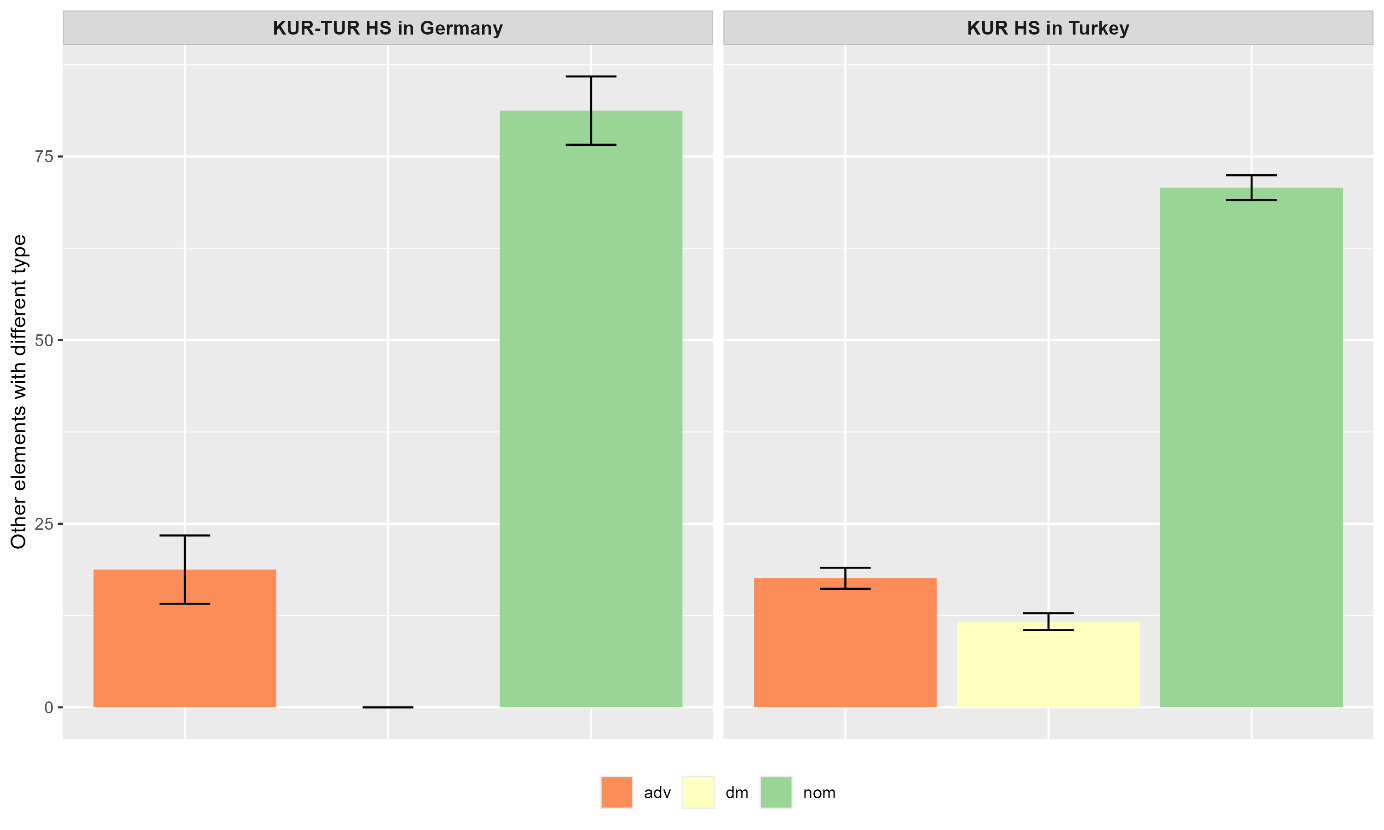
\includegraphics[width=\textwidth]{figures/iefremenko-img023.png}
\caption{\label{fig:key:25}Frequency distribution of non-goal constituents in the post-predicate position (in \%) in relation to the total number of such constituents.}
\end{figure}

\figref{fig:key:25} illustrates the frequency distribution of different types of non-goal constituents in the post-predicate position, expressed as a percentage of the total number of such constituents. The data reveals that, in both groups, non-goal constituents in the post-predicate position predominantly consist of nominal constituents. Specifically, in the data from Turkey, nominal constituents account for over 70\% (n=35) of all non-goal constituents in this position. The percentage of nominal constituents in the post-predicate position in the data from Germany is even higher, exceeding 80\% (n=13).

In addition to nominal constituents, adverbs and discourse markers also appear in the post-predicate position. Adverbs are present in both groups and are used with roughly similar frequency. Notably, Kurmanji speakers in Turkey also use discourse markers in the post-predicate position, which constitute approximately 11\% (seven examples) of the total number of non-goal elements in that context.

Overall, the analysis of the types of non-goal post-predicate elements indicates that both groups predominantly place nominal constituents in this position. While the group in Germany primarily uses nominal constituents (with 13 out of 15 examples being nominal), speakers in Turkey also incorporate adverbs and discourse markers in the post-predicate position. This distribution of non-goal elements may suggest a potential influence from the majority language on Kurmanji: in German, nominal constituents are frequently found in the post-field, while Turkish features a combination of nominal constituents, adverbs, and discourse markers in the post-predicate position, as discussed in \sectref{sec:key:5.3.2}.

\subsubsection{Semantic roles of non-goal nominal constituents in Kurmanji}\label{sec:key:6.3.6.3}

The analysis of types shows that nominal constituents are the most frequent non-goal elements in the post-predicate position. Therefore, the following section will take a closer look at their semantic roles within sentences. To this end, it will distinguish between the following types of semantic roles relevant to the data:

\begin{itemize}
\item cause


\ea \label{ex:key:88} Kurmanji, TUbi05MK\_fwK \\
\gll Şofêr-ê   erebe   pêş-iyê   li   polîs   geriya\\
driver-\textsc{ez}  car  front-\textsc{obl}  in  police  search\textsc{.pst.3sg}\\
\gll \textit{ji bo}     \textit{vî}   \textit{buyer-ê} \\
because-of  this  accident-\textsc{obl}\\
\glt ‘The driver of the front car called the police because of this incident.’ 
  \z


\item comitative (abbreviated as \textit{com} in \figref{fig:key:26}) is a person/thing that accompanies another person/thing in some action


\ea \label{ex:key:89} Kurmanji, DEtr10FK\_iwK \\
\gll Çink-ek   hawo     \textit{ba}   \textit{guddik}, \textit{ba}   \textit{torb-ok}   \textit{sew}\\
woman\textsc{-indf}  have\textsc{.pst.3sg}  with  dog   with  bag-\textsc{indf}  apple\\
‘There was a woman with a dog, with a bag of apples.’ 
  \z


\item location (abbreviated as \textit{loc} in \figref{fig:key:26} below)

\ea \label{ex:key:90} Kurmanji,  TUbi08MK\_iwK \\
\gll Qeza-yek     çêbû       hindik     manû jin-ek     bi-mîn-e   \textit{bin}   \textit{erebê}   \textit{de}\\
accident-\textsc{indf}    happen\textsc{.pst.3sg}  few    leave\textsc{.pst.3sg} woman-\textsc{indf}  \textsc{subj}-stay-\textsc{3sg}  under  car  \textsc{post}\\
\glt ‘There was an accident, and a woman was almost left under the car.’
  \z


\item source


\ea \label{ex:key:91} Kurmanji, TUbi02FK\_isK \\
\gll Ereba   a  sekinî     lê   qewimî     \textit{ji}   \textit{paşde} \\
car  hm  stop\textsc{.pst.3sg}  but  happen\textsc{.pst.3sg}  from  behind\\
\glt ‘The car stopped but bumped from behind.’ 
  \z

\item other – all other categories not mentioned above. I included different roles that occur very rarely in the data, such as possessive for example.
\end{itemize}

\begin{figure}
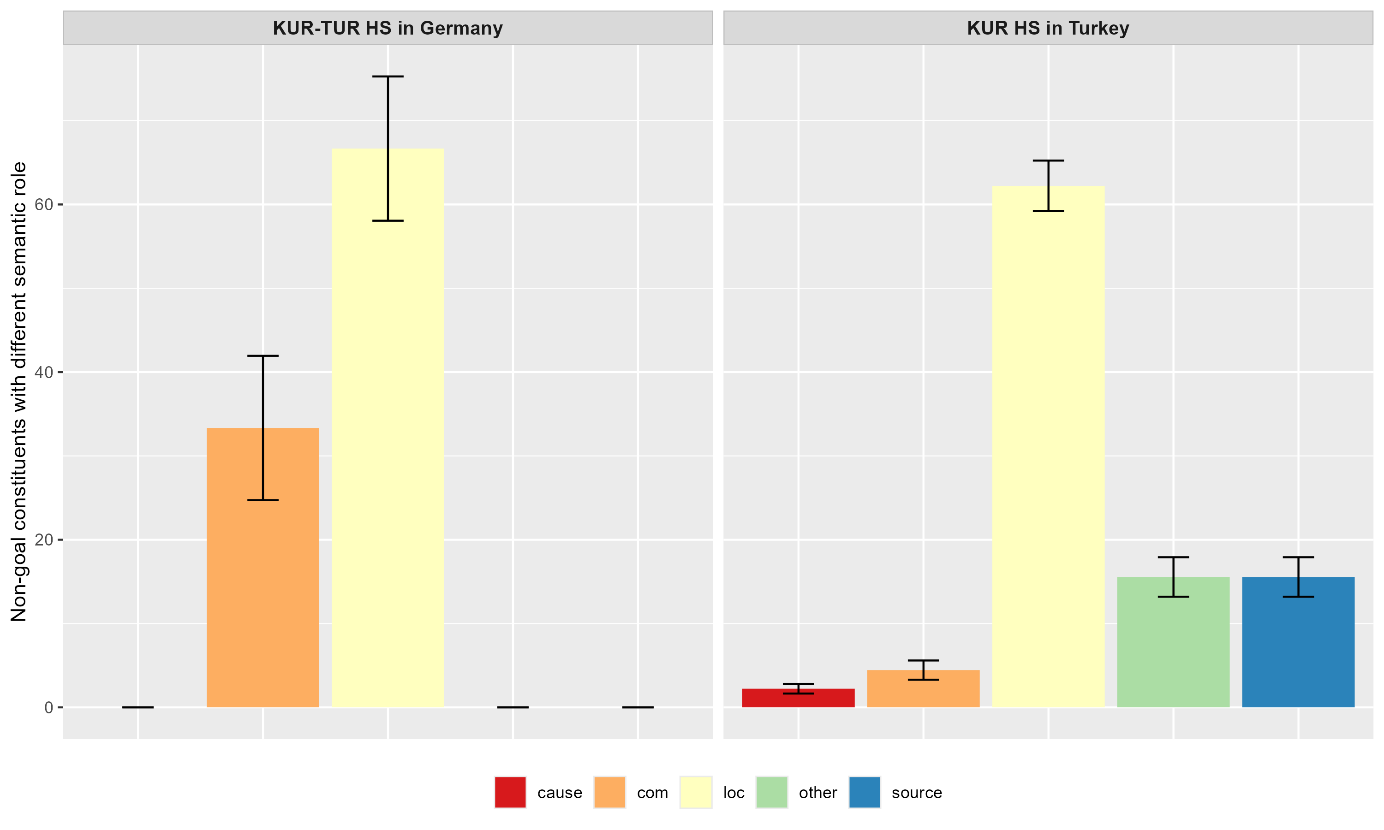
\includegraphics[width=\textwidth]{figures/iefremenko-img024.png}
\caption{\label{fig:key:26}Frequency distribution of semantic roles of non-goal arguments in the post-predicate position (in \%) in relation to the total number of such elements.}

\end{figure}

\figref{fig:key:26} illustrates the frequency of nominal non-goal post-predicate constituents categorized by their specific semantic roles, relative to the total number of nominal non-goal post-predicate constituents. It is important to interpret this distribution with caution due to the low absolute number of nominal structures in the sample.

The data reveal that the most frequently assigned semantic role for non-goal nominal constituents in the post-predicate position is location, which accounts for more than half of all examples in both groups. Additionally, in Germany, participants include constituents with a comitative role in the post-predicate position, while in Turkey, non-goal constituents are assigned various roles, including source, cause/reason, comitative, and others. The broader range of semantic roles observed in Turkey may be attributed to the larger data sample available.

Overall, the analysis of semantic roles does not reveal any significant differences between the groups. Although the absolute number of examples is low, particularly in the German data, the trends across both groups are similar. When speakers in Turkey and Germany place non-goal constituents in the post-predicate position, these constituents primarily denote locations.

\subsubsection{The use of non-goal post-predicate constituents across communicative situations}\label{sec:key:6.3.6.4}

Previous research (\citealt{Haig2014, Haig2018, Gundogdu2019}) suggests that word order in Kurmanji is influenced by predicate semantics, implying that it should not be affected by communicative situations. However, this assertion primarily pertains to goal arguments. Additionally, as mentioned in \sectref{sec:key:3.3.4}, \citet{Frommer1981} and \citet{Haig_post-predicate_EtAl2024-1} found that formality in Persian leads to an increased use of post-predicate structures. Therefore, the following discussion will explore whether formality or mode impacts the use of non-goal constituents in the post-predicate position in Kurmanji.

\begin{figure}
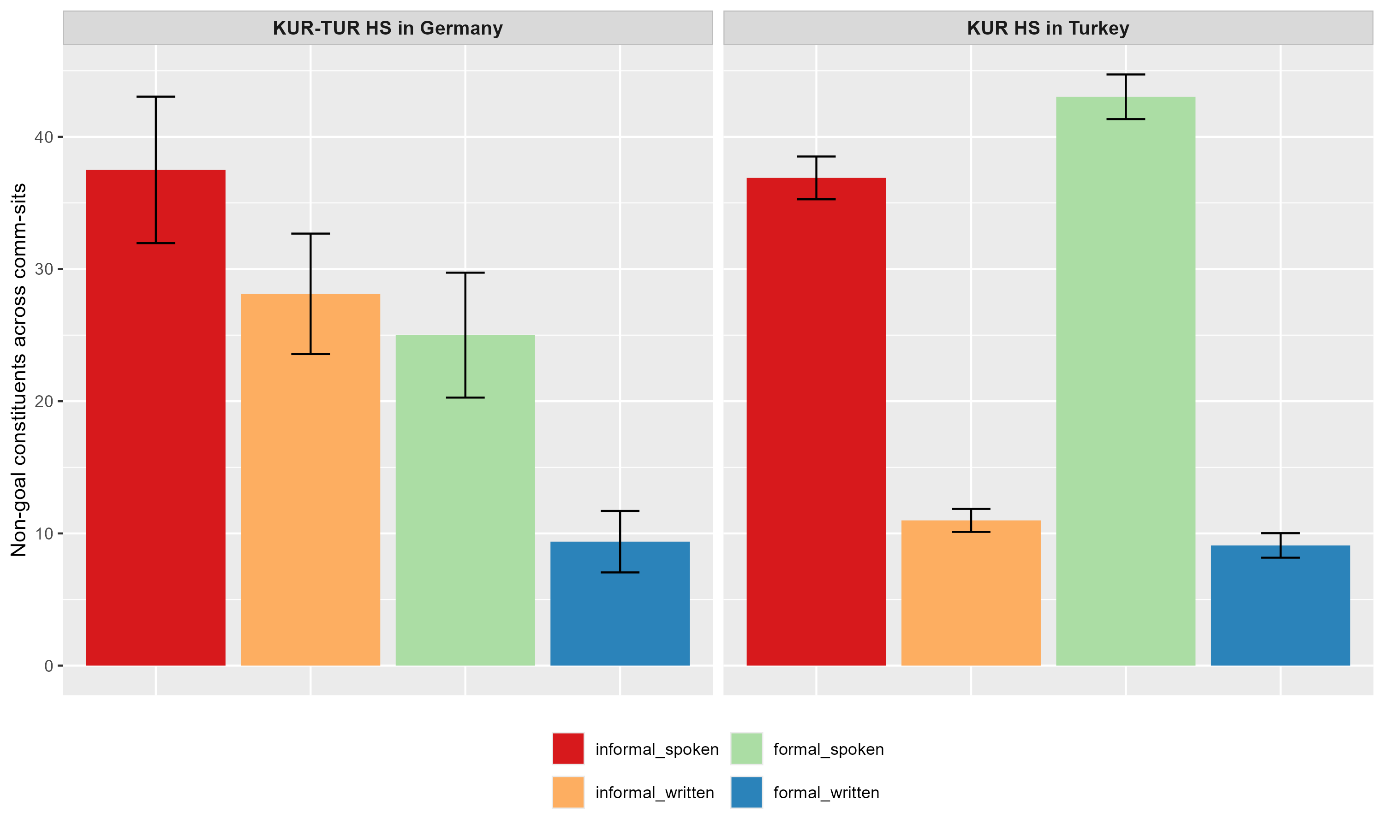
\includegraphics[width=\textwidth]{figures/iefremenko-img025.png}
\caption{\label{fig:key:27}Frequency distribution of non-goal constituents in the post-predicate position (in \%) across different communicative situations in relation to the total number of non-goal constituents.}
\end{figure}

\figref{fig:key:27} illustrates the frequency distribution of non-goal constituents in the post-predicate position relative to the total number of non-goal constituents, with error bars indicating the standard error. The data reveal that both groups use non-goal constituents across the four communicative situations. Notably, for the group in Turkey, the placement of non-goal constituents appears to be more characteristic of the spoken mode, while in Germany, informality seems to be a key predictor for the use of non-goal elements in the post-predicate position.

In summary, the qualitative analysis of non-goal constituents in the post-predicate position indicates that speakers from both groups employ constituents consisting of one or two phonological words. These non-goal elements are predominantly nominal constituents that denote location. Furthermore, the spoken mode appears to positively influence the use of non-goal constituents in the post-predicate position in Turkey, whereas informality seems to affect their placement in Germany. However, it is important to note that these observations are based on a limited number of non-goal constituents.

\section{Summary of the findings}\label{sec:key:6.4}

The current section addresses the findings on word order variation in Kurmanji varieties, specifically focusing on the post-predicate domain. As mentioned at the beginning of this chapter, Kurmanji differs from the heritage languages commonly examined in heritage language research, as it lacks a monolingual variety and does not serve as the societal majority language. Consequently, Kurmanji speakers in both Turkey and Germany are not exposed to the range of registers found in other languages. Therefore, unlike Turkish, not all factors can be analyzed within the context of Kurmanji. This discussion will focus on: \REF{ex:key:1} different language contact situations, including the various contact languages and their intensity of contact, and \REF{ex:key:2} the role of register.

First, the impact of the contact languages on Kurmanji is examined, considering the different intensity of contact between Kurmanji and Turkish compared to Kurmanji and German. The analysis begins with a quantitative analysis of post-predicate structures, revealing that Kurmanji predominantly follows a verb-final word order. On average 23.3 CUs in Germany contain a post-predicate element, compared to 14.9 CUs in Turkey. This finding aligns with previous studies on Kurmanji word order (\citealt{Haig2014}, \citealt{HaigThiele2014, Gundogdu2019}, \citealt{HaigEtAl2024}), which indicate that Kurmanji is predominantly a verb-final language.

At the same time, the data show that speakers in Germany use post-predicate structures more frequently than those in Turkey, with the analysis confirming a significant difference between the groups. However, a closer examination of the types of post-predicate constituents reveals that this increase in Germany is primarily due to a higher number of goals of motion placed in the post-predicate position. Since this position is the default for goal constituents in Kurmanji, the higher frequency of post-predicate structures in Germany may simply reflect a greater expression of motion rather than an influence from contact with German.

Next, the chapter examines the findings with a focus on the different types of constituents employed in the post-predicate position. As demonstrated in Chapter 2, Kurmanji permits three types of goals in the post-predicate position: goals of motion, addressees of verbs of speech, and recipients of verbs of transfer (\citealt{Haig2014, Gundogdu2019}). However, only the first two types appear in the dataset. This is due to the data collection method, as the video shown to participants featured a lot of movement, little interaction and practically no transfer.

An important factor influencing the position of goals in relation to the verb is the type of flagging (\citealt{Haig2014}, \citealt{HaigThiele2014, Gundogdu2019}). Goals marked with the oblique case must be placed in the post-predicate position, whereas the position of those flagged with an adposition is flexible. The only exception is locational nouns, which consistently appear in the post-predicate position because they are derived from nouns \citep{Haig2014}. Moreover, regional variation influences both the position and the types of adpositions used in Kurmanji (\citealt{Haig2014}, \citealt{Haig2022}).

The analysis of the two types of goals that occur in the data showed different results. On the one hand, the position of addressees in the data is in line with the previous research: case-flagged goals are placed in the post-predicate position and goals flagged with the help of adpositions are used in the immediate pre-predicate position. On the other hand, the analysis of goals of motion revealed that sometimes goal arguments are placed noncanonically. While case-flagged goal arguments predominantly occur in the post-predicate position, the data also reveal instances of case-flagged goals appearing in the immediate pre-predicate position.

It is important to highlight that all case-flagged goals of motion appearing in the pre-predicate position in the data from Turkey occur within the same construction, \textit{erdê ketin} (‘to fall on the ground’), where the goal argument \textit{erdê} (‘on the ground’) is placed in the noncanonical pre-predicate position. In Turkish, the contact language, \textit{erdê ketin} corresponds to \textit{yere düşmek}, a fixed construction in which the argument \textit{yere} (‘on the ground’) is consistently positioned before the verb rather than in the post-predicate position.

This pattern is further supported by mono- and bilingual Turkish data from the RUEG sub-corpora (\citealt{LudelingEtAl2024}, \citealt{IefremenkoEtAl2024}), where all instances of \textit{yere} in \textit{yere düşmek} appear before the predicate. Consequently, the noncanonical placement of \textit{erdê} in \textit{erdê ketin} may result from copying of the specific Turkish pattern \textit{yere düşmek}. Alternatively, it may stem from copying of a partially schematic pattern [N-DAT \textit{düşmek}] or a fully schematic pattern [N-DAT V] into Kurmanji.

Aside from the contact-induced explanation, the noncanonical pre-predicate position of the goal argument in \textit{erdê ketin} may also be influenced by the verb itself. In Kurmanji, \textit{ketin} appears in constructions where it functions as a light verb, losing its full lexical meaning, as seen in \textit{bi rê ketin} (‘to set off on a journey’) and \textit{li ber ketin} (‘to meet/encounter’). This could account for the higher frequency of construction copying involving \textit{ketin}, particularly when accompanied by word order changes.

As for the data from Germany, only two instances of case-flagged goal arguments appearing in the immediate pre-predicate position were observed, and neither occurred with the verb \textit{ketin}. Unlike the construction \textit{erdê ketin}, there is no clear evidence that the two noncanonically placed constructions in the German dataset—\textit{pêşiyê bazda} (‘ran ahead’) and \textit{ereba pêşiyê xist} (‘hit the front car’)—were directly copied from German.

The noncanonical placement of these arguments may be attributed to the language acquisition process among Kurmanji heritage speakers in Germany. Their parents’ Kurmanji may have already undergone structural changes due to the contact with Turkish, making these constructions part of the linguistic input provided to the next generation. Additionally, the extension of noncanonical placement to a broader range of constructions may have been reinforced by contact with German. However, drawing definitive conclusions about Kurmanji in Germany remains challenging, as the data come from only nine speakers, and the number of case-flagged goals of motion occurring preverbally is limited to just two examples.

Regarding goals marked with adpositions, previous research on Kurmanji word order indicates that their position is generally flexible, except for locational goals, which are typically restricted to the post-predicate position, similar to case-flagged goals. However, the analysis of the current data revealed instances of goals flagged with locational nouns appearing in the pre-predicate position. Notably, this noncanonical placement occurs in four examples within the Turkish dataset, three of which are used in the construction \textit{hemberî rê} (‘across the road’) with the verbs \textit{revîn} (‘to run’) and \textit{çûn} (‘to go’).

In this context, there is no direct evidence of copying a specific construction for several reasons. First, the construction \textit{hemberî rê} can be used with various verbs. Second, Turkish lacks prepositions, the equivalent construction would be rendered as \textit{yolun karşısına koşmak/gitmek}, where the spatial noun \textit{karşı} (‘opposite’) follows the noun \textit{yol} (‘road’). This suggests that the preverbal position of goal arguments flagged by locational nouns in Kurmanji may result from copying of the schematic [N-DAT V] pattern from Turkish. The findings related to CLI will be revisited in \sectref{sec:key:7.1}.

In the data from Germany, there is only one example of noncanonical argument placement flagged with a locational noun. Similar to the observations regarding case-flagged goals, this noncanonical placement differs from those found in Turkey. Notably, the construction with a preverbal goal argument was produced by the same speaker who also placed a case-flagged goal of motion in the pre-predicate position. As a result, the pre-predicate placement of goals flagged with a locational noun appears to be a characteristic specific to this individual, although it is not the only strategy employed by the speaker.

The usage-based approach underscores the significance of individual speakers in language change (\citealt{Bybee2006}, \citealt{Ansaldo2009}, \citealt{Matras2020}), suggesting that language change arises from the cumulative effects of choices made by individual speakers during their interactions. This finding therefore highlights the importance of examining individual variation, as it allows us to determine whether an innovative construction reflects an idiosyncratic preference of a single speaker or has already begun to propagate across speakers within the community. Distinguishing between these levels of variation is crucial for understanding the dynamics of change in contact settings.

Regarding the other types of adpositions, including prepositions, postpositions, circumpositions, and prepositions combined with locational nouns, the data confirm their flexible positioning. The analysis of the information status of goal arguments did not reveal a correlation between information status and the placement of adpositional goal arguments. However, the form of an adposition appears to influence its position. For instance, there is a tendency for the preposition \textit{bo} (‘to’) to be used in the post-predicate position, while \textit{li} (‘in’) is more commonly placed in the pre-predicate position.

Next, the discussion continues by examining the role of communicative situations in the employment of the post-predicate position in Kurmanji. Previous research (\citealt{Frommer1981}, \citealt{Haig_post-predicate_EtAl2024-1}) indicates a correlation between formality and mode in the use of the post-predicate position in Persian, a language that exhibits characteristics similar to other West Iranian languages. This finding for Persian suggests a possibly similar trend in Kurmanji.

Furthermore, the contact with Turkish and German may lead to the tendency of bi- and trilingual speakers to employ more post-predicate structures in the informal situations and spoken mode. However, the analysis of the frequency distribution of all post-predicate structures across the four communicative situations did not reveal any significant effect of formality or mode on the use of post-predicate structures among either group of Kurmanji speakers. Consequently, no similar developments to those observed in Turkish, German, or Persian were found.

This absence of correlation may stem from the fact that the post-predicate position in the data is primarily used for goal arguments, particularly those flagged with case, which have a fixed position and are thus less sensitive to communicative contexts. Furthermore, it is important to consider that Kurmanji is predominantly used in informal settings, and speakers do not have significant exposure to formal registers in this language.

Interestingly, in the analysis of the placement of adpositional goals of motion in Kurmanji—typically described as flexible in the literature—informality emerged as a significant factor influencing their placement. The regression analysis revealed a tendency for goals of motion flagged with an adposition to be placed in the post-predicate position in the informal situations. This correlation between formality and position may indicate developments similar to those observed in Persian (\citealt{Frommer1981}, \citealt{Haig_post-predicate_EtAl2024-1}) and could also be influenced by contact with Turkish, where the post-predicate position is common in informal situations. The role of register will be addressed in \sectref{sec:key:7.3}.

Moreover, the analysis of post-predicate constituents in Kurmanji revealed the presence of non-goal constituents in this position, with their usage being facilitated by the spoken mode among Kurmanji speakers in Turkey. This tendency can be attributed to the spontaneous nature of spoken speech, which is inherently more open to word order variation compared to the written mode, where there is more time for corrections and editing. If the spoken mode leads to an increased use of non-goal post-predicate structures in Kurmanji, a similar pattern would be expected in the data from Germany. However, the analysis of the placement of non-goal constituents across different communicative situations in Germany did not demonstrate any effect of mode. It is important to note, though, that the limited number of examples of non-goal constituents, particularly in the German data, makes it challenging to draw definitive conclusions regarding their frequency distribution across various communicative situations.

In summary, the analysis of post-predicate constituents in Kurmanji reveals that word order in both Germany and Turkey is strongly influenced by predicate semantics. The majority of post-predicate constituents consist of goals of motion and addressees of verbs of speech. While the placement of addressees is consistent with previous research, there are noncanonical examples for goals of motion. Specifically, goals flagged with case or locational nouns also occupy the pre-predicate position, particularly in certain constructions within the Turkish data. Similarly, preverbal case-flagged goal arguments and those flagged with locational nouns are found in the German data, though they appear in various constructions. Lastly, the analysis indicates that the placement of adpositional goals is flexible, with informal registers leading to the use of the post-predicate position. While non-goal constituents do occur in the post-predicate position, their frequency is low, and their usage is mainly associated with the spoken mode of Kurmanji in Turkey. This spoken mode is characterized by spontaneity and a greater openness to word order variation.


\chapter{Discussion}\label{chap:key:7}

The study aimed to attest whether the word order in the Turkish and Kurmanji varieties is undergoing change, with a specific focus on the post-predicate domain. The two languages are different in the context of heritage language research: while Turkish is one of the most vital heritage languages and has been extensively studied at least in the context of Germany, Kurmanji remains an underexplored heritage language, particularly in the German context.

This study analyzed post-predicate structures in Turkish across four groups: two Turkish heritage speaker groups in Germany—Turkish-German bilinguals and Turkish-Kurmanji-German trilinguals—and two majority Turkish speaker groups in Turkey—Turkish-Kurmanji bilinguals and Turkish monolinguals. The rich dataset for Turkish provided a valuable opportunity to investigate the impact of various factors on the use of the post-predicate position, several of which have not been thoroughly examined in the existing literature.

First, this study shifts the focus from merely comparing bilinguals to monolinguals, instead highlighting the role of societal language status—heritage versus majority. In this context, majority status includes both bilingual and monolingual speakers, while heritage status encompasses both bilinguals and trilinguals. Second, different contact situations are considered, taking into account the various contact languages involved: Kurmanji in Turkey, German in Germany, and both languages among trilingual speakers. Additionally, the intensity of contact varies across the groups. For instance, the contact between Turkish and Kurmanji began before the Ottoman Empire and intensified following the establishment of the Turkish Republic (\citealt{Yagmur2001}). In contrast, contact between Kurmanji and German emerged in the second half of the 20th century with the arrival of guest workers in Germany (\citealt{GhaderiAlmstadt2023}). Finally, as emphasized throughout this study, it is crucial to consider register when investigating heritage languages. Many phenomena examined in heritage language studies are susceptible to register variation, with certain patterns predominantly observed in formal registers. Therefore, it is essential to compare heritage speakers with appropriate data from majority speakers. In other words, comparing heritage language use in informal settings with monolingual productions in formal settings would lead to an unfair comparison that disadvantages bilingual speakers.

In the context of investigating word order in Turkish, it is particularly important to account for register variation. The use of the post-predicate position is not noncanonical per se, instead, it is typical of informal language use, while its occurrence is restricted in formal registers. Taking these arguments into account, the data for this study were collected using a method that captures the broader repertoires of speaker groups across both formal and informal settings, as well as spoken and written modes \citep{Wiese2020}. This approach was applied to all speaker groups, yielding data used across four different communicative situations among both heritage and majority speakers.

Unlike Turkish, the impact of various factors on Kurmanji cannot be thoroughly investigated. First, assessing the impact of the societal status of Kurmanji poses challenges. This study focuses on two speaker groups: Kurmanji-Turkish bilinguals in Turkey and Kurmanji-Turkish-German trilinguals in Germany. In both cases, Kurmanji is classified as a heritage language. Second, there is a scarcity of monolingual Kurmanji speakers, as most individuals are typically bilingual or multilingual, often demonstrating greater proficiency in the majority language of the country in which they reside, such as Turkish, Persian, Arabic, or other contact languages (\citealt{BrizicnodateEtAl}). Furthermore, although Kurmanji is studied in two countries with different majority languages, Turkish serves as the contact language for both groups. However, Turkish holds different societal statuses in each context: it is a majority language in Turkey and a heritage language in Germany. Additionally, the intensity of contact varies between the two language constellations, with the contact between Kurmanji and Turkish in Turkey having a much longer history than that between Kurmanji and German in Germany. Finally, this study also examines the role of register in word order variation in Kurmanji. Unlike Turkish, the use of the post-predicate position in Kurmanji is primarily influenced by predicate semantics and is not anticipated to be affected by register. However, several factors justify investigating the impact of register. First, there has been no research to date on the influence of formality and mode on word order in Kurmanji. Additionally, studies have shown how formality and mode affect word order in Persian, a language that shares syntactic features with other Western Iranian languages, including Kurmanji (\citealt{Frommer1981}, \citealt{Haig_post-predicate_EtAl2024-1}). Furthermore, in Turkish, which serves as the contact language for both groups of Kurmanji speakers in this study, the post-predicate position is related to formality and mode. Finally, as a heritage language, Kurmanji is typically not used in formal situations. Nevertheless, since speakers are likely aware of how formality and mode influence language use in the majority language, it is interesting to explore whether they develop new strategies in their heritage language to adhere to the linguistic conventions of specific communicative situations.

The main results and the underlying causes for the observed findings, along with their relation to previous studies on Turkish and Kurmanji, have been summarized at the end of Chapters 5 and 6, respectively. Given the numerous factors considered and their interplay, the main findings will be summarized in three sections: \sectref{sec:key:7.1} discusses evidence of CLI between the languages. \sectref{sec:key:7.2} explores the implications of the results for understanding internal linguistic dynamics, while \sectref{sec:key:7.3} highlights findings related to register. Finally, \sectref{sec:key:7.4} outlines the study’s limitations.

\section{Evidence of CLI on word order in Turkish and Kurmanji}\label{sec:key:7.1}

The languages under investigation here, Turkish, Kurmanji, and German, are SOV languages, but they employ the post-predicate position to a different extent. Moreover, the employment of this position is determined by different factors in the three languages: information structure in Turkish (\citealt{Erguvanli1984, Erku1983, Issever2003}), predicate semantics in Kurmanji (\citealt{Gundogdu2019, Haig2018, Haig2022}), and syntactic structure in German (\citealt{Frey2015}, \citealt{Muller2023}).

At the same time, there are also overlaps in the factors that influence the employment of the post-predicate position. Thus, for example, \citet{Asadpour2021} suggests that in addition to predicate semantics, information structure also impacts the use of the post-predicate position in Kurdish. If information structure similarly has an effect on the word order of Kurmanji spoken in Turkey, it would highlight an overlapping factor with Turkish -- information structure. Furthermore, common factors for the employment of the post-predicate position in Turkish and German are mode and formality: the post-predicate position occurs more frequently in the spoken mode compared to the written mode and in the informal language compared to the formal one (\citealt{Erguvanli1984, Schroeder2002}, \citealt{Tsehaye2023}).

Thus, the interplay of similarities and differences in these factors renders the investigated topic particularly interesting for examination in terms of CLI. This study aimed to determine whether the use of the post-predicate position varies across different language constellations in terms of frequency distribution and whether innovative factors influence its use in language contact situations. CLI refers to instances where there is evidence of one language affecting another. The societal status of the languages plays an important role in defining the direction of influence: usually a more prestigious and dominant language influences the less prestigious one. Thus, studies that investigate contact-induced language change often concentrate on minority languages. This study takes a broader approach. First, it examines Turkish in contact settings where it functions both as a heritage and a majority language. Second, it investigates potential word order changes in Kurmanji, a language in contact with Turkish. This dual focus provides deeper insights into the sources of structural changes in both languages. This section first presents evidence for CLI on heritage Turkish and heritage Kurmanji before turning to the findings on majority Turkish.

Regarding the Turkish heritage groups in Germany, the frequency analysis of post-predicate structures presented in Chapter \ref{chap:key:5} yielded mixed results. While Turkish-German bilingual speakers exhibit a frequency of post-predicate structures comparable to that of monolinguals, Turkish-Kurmanji-German trilingual speakers use them less frequently. However, a similar pattern is observed among Kurmanji-Turkish bilinguals who do not have German as a contact language, and notably, this difference emerges due to register inflexibility (see \sectref{sec:key:7.3} for further discussion). Additionally, the qualitative analysis of constituents in the post-predicate position revealed no differences between the groups. Therefore, the findings on post-predicate structures in heritage Turkish—whether among Turkish-German bilinguals or Kurmanji-Turkish-German trilinguals—do not point to the CLI from German.

With respect to Kurmanji, another heritage language under investigation, detecting and proving CLI is more challenging compared to Turkish, as monolingual Kurmanji speakers are virtually nonexistent, with most being at least bilingual. Furthermore, in both groups examined, Kurmanji is in contact with Turkish, making it difficult to establish a baseline for comparison. Therefore, as a reference point, this study draws on findings from previous research on word order in Kurmanji (\citealt{Haig2014}, \citealt{Haig2018, Gundogdu2019}), as well as studies on other Kurdish languages \citep{Asadpour2021} and Persian (\citealt{Frommer1981}, \citealt{Haig_post-predicate_EtAl2024-1}).

\largerpage
First, regarding the frequency of post-predicate structures across the groups, the analysis revealed that Kurmanji speakers in Germany use these structures more frequently than those in Turkey. However, this difference is primarily due to the more frequent placement of goals of motion in the post-predicate position among the former group. Since the post-predicate position is the canonical position for goals in Kurmanji, this distribution does not provide direct evidence for CLI from either German in Germany or Turkish in Turkey. Instead, the observed difference may simply reflect a more frequent expression of motion by the speakers in Germany.

In contrast, the qualitative analysis of goal arguments in Kurmanji indicated a structural change at the level of constructions, suggesting that word order changes are observed only in particular constructions. While the canonical position for goal arguments flagged with case or a locational noun is immediately after the predicate, there are examples in the data where such goals are placed in the pre-predicate position. This noncanonical placement occurs predominantly in certain constructions.

In Chapter \ref{chap:key:6}, it was discussed that a possible reason for the word order change at the level of constructions in Kurmanji is the influence of Turkish. One example is the construction \textit{erdê ketin} (‘to fall on the ground’), where the case-flagged argument \textit{erdê} (‘on the ground’) is placed before the predicate. This placement may be a result of the specific Turkish pattern \textit{yere düşmek}. However, there is no similar evidence for other constructions, such as \textit{hemberî rê çun/revîn} (‘to go/run to the opposite side of the road’). Thus, this suggests that the preverbal position of goal arguments marked with a locational noun in Kurmanji may be more accurately attributed to the copying of the schematic [N-DAT V] pattern from Turkish.

Similarly, the Kurmanji data from Germany revealed instances of goals marked with case or locational nouns placed in the pre-predicate position. However, unlike Turkish, no evidence suggests that these noncanonical examples in the German data resulted from copying specific or schematic constructions from German. In German, the word order follows an SOV pattern, but certain constituents, such as prepositional phrases, determiner phrases, adverbials, and adjectives, can be extraposed. Furthermore, in main declarative clauses with a finite main verb, the word order pattern is V2. Thus, while the SOV pattern in German may prompt the noncanonical placement of goals in Kurmanji, the V2 pattern might simultaneously induce the use of canonical post-predicate placement of goals in Kurmanji in Germany.

\largerpage
The baseline for Kurmanji in Germany is Kurmanji in Turkey, indicating that heritage speakers in Germany acquire the language from their bilingual parents. Findings from the data in Turkey demonstrate that Kurmanji is undergoing changes at the level of constructions, particularly with word order, showing a tendency to place goal arguments in the pre-predicate position in certain constructions. Therefore, the noncanonical placement of goal arguments observed in the German data likely does not result from contact with German, rather, these constructions were already present in the language of the parents and were subsequently acquired by heritage speakers in Germany.\footnote{{Although, in order to prove that the noncanonical position of goals is already present in the input received by the heritage speakers of Kurmanji in Germany, it is necessary to collect data from the parents of the speakers.}}

At the same time, the absence of direct influence from German on Kurmanji syntax may be attributed to the focus on noncanonical constructions. The V2 structure in German could also induce the canonical [V N-DAT] pattern in Kurmanji. It is important to note that the frequency analysis revealed a higher number of goal arguments in the post-predicate position in the data from Germany compared to that from Turkey. This observation may indeed reflect the influence of the majority language, German, on the stability of Kurmanji syntax.

Furthermore, the systematic observation of noncanonical placement of goal arguments in the same constructions in the data of several speakers from Turkey indicates that this pattern is not merely an error. Instead, these innovative constructions appear to be in the process of propagation. Both constructions—those with arguments in the pre-predicate and post-predicate positions—are firmly established in individual speakers’ minds, and it remains unclear whether the innovative construction will ultimately supplant the canonical one.

In contrast, the number of noncanonical constructions in the data from Germany is limited, with only three examples in total, two of which originate from the same speaker. Consequently, there is no evidence of propagation for these innovative constructions in Germany. However, it is important to reiterate that the dataset from Germany is small. Therefore, to determine whether the innovative pattern is used by a wider range of speakers and whether it extends to additional constructions, further data collection from Kurmanji heritage speakers in Germany is necessary.

The results outlined above pertain to innovative developments in the post-predicate domain in heritage Turkish and heritage Kurmanji. In addition to examining these heritage languages, the study also explored Turkish as the majority language of Kurmanji-Turkish bilinguals and Turkish monolinguals in Turkey. The analysis revealed that Kurmanji-Turkish bilinguals use fewer post-predicate structures compared to Turkish monolinguals. Notably, a similar pattern in frequency distribution was observed among the Turkish data from the Kurmanji-Turkish-German trilingual group in Germany.

This difference in frequencies could suggest a CLI from Kurmanji, which is predominantly a verb-final language. However, a detailed analysis of post-predicate structures indicates that the frequency differences between the groups with and without Kurmanji as a contact language do not stem from such influence. Firstly, the qualitative analysis of post-predicate structures in both groups showed no evidence of CLI at the construction level. For example, verb arguments—such as goals of motion, addressees of verbs of speech, and recipients of verbs of transfer—that are systematically placed in the post-predicate position in Kurmanji do not occur more frequently in that position in Turkish among groups where Kurmanji serves as the contact language compared to those without it. Secondly, the analysis demonstrated that differences in the frequency distribution of post-predicate structures between the groups with and without Kurmanji as a contact language primarily result from register inflexibility (see \sectref{sec:key:7.3} for further discussion). If CLI from Kurmanji on Turkish were present, one would expect to see fewer post-predicate structures in groups where Kurmanji is the contact language across all communicative situations. However, since this is not the case, the observed differences in frequency cannot be attributed to the CLI.

In summary, the analysis found no evidence of CLI between the recently contacted languages, specifically heritage Turkish and Kurmanji in relation to German. Regarding the longer-standing contact between Turkish and Kurmanji, the societal status of the languages significantly influences the direction of that influence. The analysis did not reveal evidence of CLI in majority Turkish. However, it indicated that Kurmanji, as a heritage language, is experiencing CLI from Turkish, evidenced by changes in word order at the construction level.

According to the usage-based approach, change in syntax is the result of the change of many constructions, which are not spontaneous, but systematic changes. The data indicate that word order changes at the construction level are in the process of propagation in Turkey, as noncanonical constructions are used by different speakers. However, these novel constructions do not yet surpass canonical constructions in frequency, leaving it uncertain whether the noncanonical patterns will eventually dominate. In contrast, the data from Germany show only a few noncanonical constructions, suggesting no evidence of propagation for these innovative structures in that context. Nonetheless, any claims regarding Kurmanji in Germany remain tentative, as the dataset is too small to draw definitive conclusions.

\section{Internal dynamics: Is monolingual Turkish undergoing change?}\label{sec:key:7.2}

Apart from the contact situations, the investigation also focused on the monolingual variety, although only of Turkish. As previously explained, Kurmanji speakers are typically bilingual or multilingual, therefore, data from monolingual Kurmanji speakers are unavailable.

The analysis revealed several internal developments occurring in Turkish. First, the examination of the information status of referents in the post-predicate position indicated that monolingual speakers also place new referents in this position. This finding contradicts the assertions made in descriptive grammars of Turkish, which state that new information is not permitted in the post-predicate position (\citealt{Erguvanli1984, GokselÖzsoy2000, Issever2003}).

However, it was observed that most instances of new referents in the post-predicate position included secondary information about a nominal referent previously introduced in the pre-predicate position. Although research on this development in Turkish is limited, several studies have noted that new information can be placed in the post-predicate position if it is deemed less important compared to the new information introduced in the pre-predicate position (\citealt{DogruozBackus2007}, \citealt{AkanHartmann2019, Issever2019}). Additionally, the current study indicates that new elements in the post-predicate position occur in monolinguals, but primarily in informal contexts. This finding may suggest the initial stages of change within the language of monolingual speakers, however, it remains uncertain whether this will lead to a loosening of the information structural constraints in the future.

The second development concerning monolingual Turkish involves the use of post-predicate structures in formal situations. The study revealed that the post-predicate position is characteristic not only of informal settings, as stated by \citet{Erguvanli1984}, but is also frequently used in formal situations, particularly in spoken mode. It is important to note that this finding cannot be generalized across all formal spoken communicative situations in Turkish. The formal spoken production analyzed in this study comes from an oral witness report made to a police answering machine, where participants had to respond spontaneously without preparation. In contrast, more planned and prepared formal spoken situations, such as conference talks, news reports, or lectures, may contain significantly fewer post-predicate structures than an oral witness report. Future research is needed to gain a deeper understanding of the use of the post-predicate position across various formal registers.

\section{The role of register in heritage language research}\label{sec:key:7.3}

\largerpage
When comparing two or more speaker groups, selecting the appropriate baseline is crucial. This consideration is particularly important in the context of heritage languages, which are typically acquired at home in informal settings. Heritage speakers often have limited exposure to formal registers of their heritage language, as they frequently do not receive education in that language. Consequently, comparing spoken data collected from informal situations in a heritage language to the norms of a standard language may present a distorted view of developments in the heritage language \citep{WieseEtAl2022}. For instance, differences between the two may be mistakenly attributed to incomplete acquisition, attrition, or contact-induced language change. In reality, the observed differences between heritage and majority varieties might stem from register inflexibility in heritage speakers. The term \textit{register flexibility} is usually discussed in the context of foreign language learning, where register flexibility is defined as “the ability to flexibly use a variety of linguistic resources – at the lexical, syntactic and discourse levels, with the awareness of which are the most appropriate for the communicative contexts at hand” (\citealt{QinUccelli2020}).

Taking these considerations into account, the data for this study were collected using a method designed to capture the broader repertoires of speaker groups across both formal and informal settings in spoken and written modes \citep{Wiese2020}. As previously mentioned, \citet{SchroederEtAl2024} employed the same method to investigate the post-predicate position among Turkish heritage speakers in Germany and the US, finding evidence of register inflexibility in the latter group. Specifically, US speakers used the post-predicate position frequently in both informal and formal situations, whereas monolinguals typically employed this structure only in informal situations and spoken modes. However, no lack of register flexibility was identified among heritage speakers in Germany.

Consistent with the findings of \citet{SchroederEtAl2024}, the analysis of the current data did not reveal register inflexibility among Turkish heritage speakers in Germany in terms of the frequency distribution of post-predicate structures. However, this conclusion applies only to bilingual Turkish heritage speakers in Germany, who use significantly higher number of post-predicate structures in the informal situations compared to the formal ones, as well as in spoken mode versus written mode.

In terms of the frequency distribution of post-predicate structures, both overall and across various communicative situations, the data reveal differences between the groups with and without Kurmanji as the contact language. While Turkish monolinguals and Turkish heritage speakers in Germany show clear distinctions across communicative situations, Turkish bilingual speakers in Turkey show no significant differences regarding formality, and Kurmanji-Turkish heritage speakers in Germany exhibit no significant differences in either formality or mode. This pattern observed among Kurmanji speakers in both Germany and Turkey may suggest register inflexibility, where the distinctions between formal and informal situations, as well as between spoken and written language, become less pronounced.

First, the difference between the two heritage speaker groups in Germany is interesting: bilingual heritage speakers distinguish between different registers, while trilingual speakers do not. This variation may be attributed to their differing levels of exposure to and use of heritage Turkish. Bilingual speakers are exposed to Turkish at home and in informal public settings, particularly in Berlin, whereas trilingual speakers are also exposed to Kurmanji in addition to Turkish. However, establishing a correlation between the amount of input and exposure and the employment of post-predicate constituents in the different communicative situations falls outside the scope of this study.

Another contributing factor could be the different input received by the two groups: trilingual speakers acquire their heritage languages from their Kurmanji-Turkish bilingual parents. As the analysis has shown, the Turkish of Kurmanji-Turkish bilinguals is predominantly verb-final.  Furthermore, it is important to consider that the trilingual speaker group consists of only nine individuals, thus, increasing the sample size could potentially impact the observed frequency distribution.

At the same time, the difference between the two majority speaker groups merits attention. That is, monolingual majority speakers differentiate between formal and informal, as well as spoken and written communicative situations regarding their use of the post-predicate position. In contrast, Turkish bilingual speakers in Turkey do not exhibit significant differences based on formality. This frequency distribution suggests register inflexibility among bilingual majority speakers. However, this register inflexibility differs from what \citet{SchroederEtAl2024} observed in heritage speakers in the US, where Kurmanji-Turkish bilinguals use a greater number of structures typical of formal language in informal situations.

There are two potential explanations for the differences between the groups. First, Kurmanji-Turkish bilinguals in Turkey are largely exposed to Turkish in formal environments, while they primarily use Kurmanji with family members and some friends. As a result, the entrenchment of preverbal constructions is high among these speakers, influenced not only by the frequent SOV pattern in Kurmanji but also by their exposure to predominantly preverbal structures in formal Turkish situations.

Another reason may stem from the canonical behavior of bilingual speakers when using their majority language. Although research on the majority language use of heritage speakers is limited, evidence suggests that bilinguals tend to be more explicit and favor formal language and canonical structures when speaking their majority language (\citealt{SevincDewaele2018}, \citealt{Bunk2024, bunk_anxious_2025}). Studies indicate that monolingual habits and standard language ideologies can induce language anxiety in bilingual individuals, which may in turn lead to specific linguistic behaviors, such as the use of formal language in informal situations. As \citet{Bartholoma2021} indicates, language ideology in Turkey is often described as a `monoglot' ideology (for the term see \citealt{Silverstein1996}), which denies the existence of multilingualism within its borders and further restricts the use of non-state languages in both public and private spheres. This ideology embraces the notion of `one country, one language' and seeks to protect the state language from the influence of foreign and minority languages.

While there are no systematic studies on the societal perception of Turkish as spoken by bilingual speakers in Turkey, there is a recognized bias against Kurmanji-Turkish bilinguals, with the belief that their language does not conform to the norms of Standard Turkish. Additionally, several studies indicate that bilingual speakers in Turkey experience language anxiety (\citealt{Sahin-firat2010, Tulgar2010}). As a result, the use of formal markers and canonical language in the informal situations by bilinguals in Turkey might be the result of their wish to show the ability to speak the language “properly”.

Furthermore, register inflexibility was observed not only based on the general frequency distribution of post-predicate structures but also in the analysis of the information status of referents. The findings revealed that both heritage and majority Turkish speakers in Germany and Turkey place new referents in the post-predicate position, with heritage speakers doing so significantly more often. However, while majority speakers typically do this only in informal situations, heritage speakers employ this structure across all communicative contexts. As a result, the more frequent placement of new referents in the post-predicate position by heritage speakers can be attributed to register inflexibility.

As for Kurmanji, investigating language variation across communicative situations presents an interesting and innovative perspective. Unlike Turkish, there is no opposition between heritage and majority Kurmanji. Moreover, the language is used predominantly in informal situations, at least in Turkey. For instance, formal procedures like speaking to the police or writing a witness report are conducted in Turkish, not Kurmanji. Hence, Kurmanji-Turkish bilingual speakers are basically never exposed to Kurmanji in formal situations. However, they are likely aware of register variation in languages, owing to the knowledge they receive in Turkish. Thus, it is interesting to see whether speakers implement their register knowledge also in their heritage language, thereby creating novel strategies in the formal situations of Kurmanji.

Furthermore, as noted several times, no study has specifically investigated the use of the post-predicate position in Kurmanji across different communicative situations, at least to the best of our knowledge. Although research on Persian has demonstrated that a lower degree of formality corresponds with an increase in post-predicate elements (\citealt{Frommer1981}, \citealt{Haig_post-predicate_EtAl2024-1}).

The analysis of the Kurmanji data revealed that the frequency distribution of post-predicate structures showed no effect of communicative situations. This finding suggests that the phenomenon under investigation is not sensitive to formality or mode in Kurmanji, rather, it is linked to predicate semantics. However, in structures where previous research (\citealt{Haig2014, Gundogdu2019}) indicated potential variation—specifically regarding the position of goals marked with an adposition—the analysis found that formality does indeed influence the placement of such structures. Goals flagged with an adposition are favored in the post-predicate position in the informal situations. This preference for the post-predicate position mirrors patterns observed in Turkish. This suggests that when variation is possible in the heritage language, speakers may be inclined to adopt strategies known from the majority language.

Finally, the analysis of the Kurmanji data revealed that, in addition to goal arguments, non-goal constituents are also placed in the post-predicate position. An examination of the frequency of these constituents across communicative situations indicated that the spoken mode particularly facilitates their use in Kurmanji spoken in Turkey. A similar pattern has been observed in Turkish, where the spoken mode positively impacts the use of the post-predicate position. As previously mentioned, the spontaneous nature of spoken language allows for greater word order variation, whereas the written mode offers opportunities for corrections and adjustments. However, interpreting the results for the distribution of non-goal constituents across communicative situations should be approached with caution, as the total count of these structures is relatively low.

\section{Limitations of the study}\label{sec:key:7.4}

While the study provides an in-depth exploration of the topic, several limitations should be acknowledged. First of all, as emphasized several times, the data from the trilingual group in Germany comes from nine speakers. For this reason, the conclusions about this group are mainly drawn from qualitative patterns rather than statistical analyses. For future research, more data need to be collected from the trilingual group. Besides, another group could be added to the study, that is Kurmanji-German bilinguals, who do not have Turkish in their repertoire. Adding this group could shed light on the contact-induced language change in Kurmanji in Germany.

Another limitation, and at the same time a direction for future research, concerns the range of communicative situations investigated. First, the categorization of police reports as formal and messages to a friend as informal could be regarded as somewhat simplistic. In order to determine whether the findings can be generalized to formal and informal communicative situations more broadly, future research should replicate the study using a wider range of communicative contexts. Moreover, \citet{Maas2010} differentiates between informal registers in private and public contexts. An illustration of a private informal register is communication within family and friends, whereas a public informal register encompasses everyday interactions at workplaces, markets, streets, and similar settings. Thus, it would be interesting to investigate the use of the post-predicate position also in public informal registers. Besides, the study showed that the use of post-predicate structures in Turkish is also high in the formal communicative situation but only in the spoken mode. However, it is interesting to investigate whether such a finding is relevant for all formal spoken communicative situations or only for spontaneous formal speech. Hence, the investigation of the formal spoken communicative situations prepared in advance, such as a talk at a conference, a lecture, can be made.

Furthermore, for the analysis of the information status of post-predicate constituents, it is important to remember that the data from the four communicative situations were analyzed. Hence, the concept of ‘given’ and ‘new’ within one communicative situation might overlap in scenarios where a speaker has already narrated the story once, twice, or even more times. Thus, the information status of the constituents should be investigated with data that was not narrated several times. Another alternative is to use a different stimulus for the elicitation of different communicative situations.

Finally, while the analysis of post-predicate elements provides a detailed account of their weight, constituent types, semantic roles, the study does not examine the properties of constituents occurring in the pre-predicate position. Consequently, it is not possible to assess which types of constituents appear pre-predicatively or how their distribution relates to the patterns observed post-predicatively. Future research should therefore include a systematic analysis of constituents in the pre-predicate position in order to provide a more complete picture of constituent distribution.


\chapter{Understanding heritage speakers’ languages: Conclusion and outlook}\label{chap:key:8}

This study investigated heritage speakers’ languages by examining various factors that contribute to differences between heritage and majority languages, with a particular focus on word order in Turkish and Kurmanji in Germany and Turkey. As outlined in the introduction, research on heritage languages lacks linguistic diversity, with the majority of existing studies concentrating on languages such as Spanish and Chinese in contact with English. By focusing on Turkish and Kurmanji, the present study contributes to broadening the empirical scope of heritage language research.

While Turkish as a heritage language has received considerable attention, particularly in the German context, heritage Kurmanji remains virtually unexplored. Research on Kurmanji-Turkish bilinguals is also extremely limited, both with respect to their Kurmanji and their Turkish. The present study addresses this gap by providing the first systematic investigation of Kurmanji as a heritage language in Germany and by examining both Kurmanji and Turkish among Kurmanji-Turkish bilingual speakers.

Although \citegen{Rothman2009} definition of a heritage language encompasses a broad spectrum of speakers and languages worldwide, research on heritage languages is often limited to immigration contexts, particularly in Europe and North America. By including Kurmanji-Turkish bilinguals, the study challenged the often implicit assumption that heritage speakers are primarily associated with immigrant languages in the Global North. It highlighted the importance of recognizing linguistic diversity among heritage speakers, including speakers of minoritized languages.

The study built on existing proposals that aim to explain why heritage languages differ from majority languages, with a particular focus on transfer and divergent attainment accounts. To explore the divergent attainment account more comprehensively, the study examined not only commonly investigated factors such as cross-linguistic influence and bilingualism, but also the societal status of the languages, internal linguistic dynamics, particularly concentrating on the role of register.

Heritage language research often compares bilingual heritage speakers with monolingual majority speakers, thereby investigating two factors simultaneously: bilingualism and the societal status of the language. To disentangle these factors, the study included an additional group of speakers—Kurmanji-Turkish bilinguals in Turkey. While these speakers are bilingual, like heritage speakers, Turkish in this context is not a heritage language but the majority language.

Adding this group introduced another parameter: the intensity of contact. In Germany, contact between Turkish or Kurmanji and the dominant German language began in the late 20th century with the arrival of ‘guest workers,’ while Turkish-Kurmanji contact dates back to the Ottoman Empire and intensified with the establishment of the Turkish Republic (Yağmur 2001). The intensity of contact appears to play a significant role in the factors driving differences between the groups. Transfer was observed only in the Kurmanji spoken in Turkey, where language contact has been ongoing for years. In contrast, no trace of cross-linguistic influence was found in heritage Turkish or heritage Kurmanji spoken in Germany.

That said, the statement that no transfer is observed in more recent contact situations refers, of course, only to the phenomenon investigated in this study and does not rule out the possibility of transfer from the dominant language in more recent contact situations. Undoubtedly, such transfer exists, and extensive research provides ample evidence of this phenomenon, as shown in Chapter \ref{chap:key:1}.

The key point here is that other factors must also be explored. This study specifically highlighted the role of internal dynamics in the language, including changes in the (monolingual) majority variety that are unrelated to language contact. To observe such dynamics, however, it is essential to collect and analyse the informal speech of the majority language speakers. For example, the study revealed that noncanonical phenomena, such as the placement of new referents in the post-predicate position, are also found in the informal registers of majority Turkish speakers. Without collecting data from different registers, it would not have been possible to attest these ongoing differences in the monolingual variety.

Second, incorporating register into the analysis of heritage language use made it possible to identify more precisely the contexts in which heritage speakers diverge from majority language speakers. When the frequency of placing new information in the post-predicate position was examined without taking register differences into account, the results suggested that this noncanonical phenomenon occurs much more frequently among heritage speakers than among majority speakers. However, a closer examination of new information placement across different communicative situations revealed that this apparent frequency difference stems from a lack of register flexibility in heritage speakers. Specifically, while majority speakers tend to place new information in the post-predicate position only in informal settings, heritage speakers do so across all communicative situations, without distinguishing between formal and informal settings. Such a finding is unsurprising, given the conditions under which heritage languages are acquired—primarily at home, with limited or no access to formal education in the language.

The finding that differences between heritage and majority speakers primarily manifest in formal registers supports the proposal centered on divergent attainment in heritage speakers. Heritage speakers acquire their language in a context different from that of majority speakers, often without formal education in the language. As a result, they exhibit less flexibility in formal registers. This finding also emphasizes the crucial need to provide opportunities for heritage speakers to engage with the formal registers of their heritage language and highlights the importance of ensuring that heritage languages are included in school curricula, expanding the number of language classes available, developing textbooks, and creating all possibilities for learning all languages, not just the ones that are traditionally considered prestigious. Implementing such measures would foster a more inclusive and equitable language education that fully embraces linguistic diversity.

Furthermore, the study also revealed that register inflexibility concerns not only heritage speakers but also speakers of the majority languages. However, unlike the extension of features typical of informal language into formal situations observed in heritage speakers, majority language speakers tend to employ more formal language even in informal situations. Such register inflexibility may stem from language anxiety experienced by bilingual speakers, even when communicating in their majority language (\citealt{SevincDewaele2018}, \citealt{Bunk2024}). The reason for this is strong monolingual habitus which takes monolingualism as the norm and does not welcome any foreign influence on the language (\citealt{Wiese2020}, \citealt{KerswillWiese2022}). The register inflexibility attested in the majority language emphasizes the importance of embracing multilingualism and abandoning the idea that monolingualism is the norm, especially considering that the majority of the world’s population is multilingual.

Future research on heritage speakers should consider register as one of the factors and explore other linguistic domains and language phenomena to determine whether what was previously attributed to cross-linguistic influence could, in fact, stem from register inflexibility in bilinguals. Much of the research conducted in the RUEG project has already addressed this (\citealt{AlexiadouRizou2023}, \citealt{WieseEtAl2022}, \citealt{Tsehaye2023}, \citealt{SchroederEtAl2024}). Additionally, the RUEG corpora (\citealt{LudelingEtAl2022}, \citealt{IefremenkoEtAl2024}) available online can be used for further research, providing an opportunity to investigate the role of register in bilinguals.

Furthermore, little is known about the role register plays in the processing of language by speakers. A limited but emerging body of research has examined how monolingual speakers process (mis)matches in formality/register (\citealt{MaquateEtAl2025}, \citealt{PescumaEtAl2024}), yet comparable evidence for bilingual populations remains largely absent. This gap is currently being addressed within the Collaborative Research Centre 1412 “Register: Language Users’ Knowledge of Situational-Functional Variation” (CRC 1412), a DFG-funded research centre based in Germany. The CRC investigates register from multiple linguistic perspectives; within this framework, one subproject focuses specifically on the real-time processing of register mismatches among heritage speakers in Germany.

At the same time, it is important to acknowledge that not every heritage language can be explored through such a broad range of factors. As mentioned earlier, a heritage language is not necessarily one spoken by the children or grandchildren of immigrants to the Global North. Many minoritized languages exhibit the characteristics of a heritage language. However, such languages may lack a monolingual variety because often speakers of these minority languages tend to be bilingual or even multilingual, with a dominant proficiency in the societal language of the region they live in. As a result, these minority languages typically do not have a majority variety, and consequently, may not possess a wide range of registers, or at least speakers are often not exposed to or do not have opportunities to engage with these different registers.

Recognizing these complexities highlights the importance of broadening the scope of heritage language research. To truly understand heritage speakers' languages and model their grammar, it is crucial to include a diverse range of languages and language pairs. This approach would foster dialogue between studies on minoritized languages and heritage language research, fields that, while addressing similar issues, often operate in isolation from one another. Building on these considerations, the present study took a step toward bridging this gap by positioning Kurmanji as a heritage language in Turkey and contributed to research on both heritage Kurmanji and majority Turkish among Kurmanji-Turkish bilinguals. Furthermore, by making the corpus data openly accessible, the study aimed to encourage further research on these language pairs and to foster broader engagement with languages that have traditionally been underrepresented in heritage language research.


% % copy the lines above and adapt as necessary

%%%%%%%%%%%%%%%%%%%%%%%%%%%%%%%%%%%%%%%%%%%%%%%%%%%%
%%%             Backmatter                       %%%
%%%%%%%%%%%%%%%%%%%%%%%%%%%%%%%%%%%%%%%%%%%%%%%%%%%%
 
%\input{localseealso.tex}  
% There is normally no need to change the backmatter section
\sloppy
\backmatter 
\phantomsection%this allows hyperlink in ToC to work
\printbibliography[heading=references] 
\cleardoublepage
\phantomsection
\addcontentsline{toc}{chapter}{\lsIndexTitle}
\addcontentsline{toc}{section}{\lsNameIndexTitle}
\ohead{\lsNameIndexTitle}
\printindex
\cleardoublepage
  
% \phantomsection 
% \addcontentsline{toc}{section}{\lsLanguageIndexTitle}
% \ohead{\lsLanguageIndexTitle} 
% \printindex[lan] 
% \cleardoublepage
  
% \phantomsection 
% \addcontentsline{toc}{section}{\lsSubjectIndexTitle}
% \ohead{\lsSubjectIndexTitle} 
% \printindex[sbj]
% \ohead{} 


 
\end{document} 
